% *** Authors should verify (and, if needed, correct) their LaTeX system  ***
%DIF LATEXDIFF DIFFERENCE FILE
%DIF DEL R1-Tsallis_entropy_sar.tex   Tue May 12 13:03:36 2026
%DIF ADD R2-Tsallis_entropy_sar.tex   Fri Jun 26 14:52:18 2026
% *** with the testflow diagnostic prior to trusting their LaTeX platform ***
% *** with production work. IEEE's font choices can trigger bugs that do  ***
% *** not appear when using other class files.                            ***
% The testflow support page is at:
% http://www.michaelshell.org/tex/testflow/


%%*************************************************************************
%% Legal Notice:
%% This code is offered as-is without any warranty either expressed or
%% implied; without even the implied warranty of MERCHANTABILITY or
%% FITNESS FOR A PARTICULAR PURPOSE!
%% User assumes all risk.
%% In no event shall IEEE or any contributor to this code be liable for
%% any damages or losses, including, but not limited to, incidental,
%% consequential, or any other damages, resulting from the use or misuse
%% of any information contained here.
%%
%% All comments are the opinions of their respective authors and are not
%% necessarily endorsed by the IEEE.
%%
%% This work is distributed under the LaTeX Project Public License (LPPL)
%% ( http://www.latex-project.org/ ) version 1.3, and may be freely used,
%% distributed and modified. A copy of the LPPL, version 1.3, is included
%% in the base LaTeX documentation of all distributions of LaTeX released
%% 2003/12/01 or later.
%% Retain all contribution notices and credits.
%% ** Modified files should be clearly indicated as such, including  **
%% ** renaming them and changing author support contact information. **
%%
%% File list of work: IEEEtran.cls, New_IEEEtran_how-to.pdf, bare_jrnl_new_sample4.tex,
%%*************************************************************************
\PassOptionsToPackage{unicode}{hyperref}
\PassOptionsToPackage{hyphens}{url}
\PassOptionsToPackage{dvipsnames,svgnames,x11names}{xcolor}
% Note that the a4paper option is mainly intended so that authors in
% countries using A4 can easily print to A4 and see how their papers will
% look in print - the typesetting of the document will not typically be
% affected with changes in paper size (but the bottom and side margins will).
% Use the testflow package mentioned above to verify correct handling of
% both paper sizes by the user's LaTeX system.
%
% Also note that the "draftcls" or "draftclsnofoot", not "draft", option
% should be used if it is desired that the figures are to be displayed in
% draft mode.
%
\documentclass[
  lettersize  journal,
]{IEEEtran}%
% If IEEEtran.cls has not been installed into the LaTeX system files,
% manually specify the path to it like:
% \documentclass[journal]{../sty/IEEEtran}
%\usepackage[cmex10]{amsmath}
%\usepackage{amssymb}
\usepackage{iftex}
\usepackage{subcaption}
\renewcommand{\thesubfigure}{(\alph{subfigure})}
\captionsetup[subfigure]{labelformat=simple}
\usepackage{caption}
\captionsetup[table]{justification=centerlast, labelsep=newline, textfont={small,sc}}
\ifPDFTeX
  \usepackage[T1]{fontenc}
  \usepackage[utf8]{inputenc}
  \usepackage{textcomp} % provide euro and other symbols
\else % if luatex or xetex
  \usepackage{unicode-math} % this also loads fontspec
  \defaultfontfeatures{Scale=MatchLowercase}
  \defaultfontfeatures[\rmfamily]{Ligatures=TeX,Scale=1}
\fi
%\usepackage{lmodern}
\ifPDFTeX\else
\fi
% Use upquote if available, for straight quotes in verbatim environments
\IfFileExists{upquote.sty}{\usepackage{upquote}}{}
\IfFileExists{microtype.sty}{% use microtype if available
  \usepackage[]{microtype}
  \UseMicrotypeSet[protrusion]{basicmath} % disable protrusion for tt fonts
}{}
\makeatletter
\parindent    1.0em
\ifCLASSOPTIONcompsoc
  \parindent    1.5em
\fi
\makeatother
\usepackage{xcolor}
\setlength{\emergencystretch}{3em} % prevent overfull lines

\setcounter{secnumdepth}{5}
% Make \paragraph and \subparagraph free-standing
\ifx\paragraph\undefined\else
  \let\oldparagraph\paragraph
  \renewcommand{\paragraph}[1]{\oldparagraph{#1}\mbox{}}
\fi
\ifx\subparagraph\undefined\else
  \let\oldsubparagraph\subparagraph
  \renewcommand{\subparagraph}[1]{\oldsubparagraph{#1}\mbox{}}
\fi

\usepackage{longtable,booktabs,array}
\usepackage{calc} % for calculating minipage widths
% Correct order of tables after \paragraph or \subparagraph
\usepackage{etoolbox}
\makeatletter
\patchcmd\longtable{\par}{\if@noskipsec\mbox{}\fi\par}{}{}
\makeatother
% Allow footnotes in longtable head/foot
\IfFileExists{footnotehyper.sty}{\usepackage{footnotehyper}}{\usepackage{footnote}}
\makesavenoteenv{longtable}
\usepackage{graphicx}
\makeatletter
\newsavebox\pandoc@box
\newcommand*\pandocbounded[1]{% scales image to fit in text height/width
  \sbox\pandoc@box{#1}%
  \Gscale@div\@tempa{\textheight}{\dimexpr\ht\pandoc@box+\dp\pandoc@box\relax}%
  \Gscale@div\@tempb{\linewidth}{\wd\pandoc@box}%
  \ifdim\@tempb\p@<\@tempa\p@\let\@tempa\@tempb\fi% select the smaller of both
  \ifdim\@tempa\p@<\p@\scalebox{\@tempa}{\usebox\pandoc@box}%
  \else\usebox{\pandoc@box}%
  \fi%
}
% Set default figure placement to htbp
\def\fps@figure{htbp}
\makeatother


% definitions for citeproc citations
\NewDocumentCommand\citeproctext{}{}
\NewDocumentCommand\citeproc{mm}{%
  \begingroup\def\citeproctext{#2}\cite{#1}\endgroup}
\makeatletter
 % allow citations to break across lines
 \let\@cite@ofmt\@firstofone
 % avoid brackets around text for \cite:
 \def\@biblabel#1{}
 \def\@cite#1#2{{#1\if@tempswa , #2\fi}}
\makeatother
\newlength{\cslhangindent}
\setlength{\cslhangindent}{1.5em}
\newlength{\csllabelwidth}
\setlength{\csllabelwidth}{3em}
\newenvironment{CSLReferences}[2] % #1 hanging-indent, #2 entry-spacing
 {\begin{list}{}{%
  \setlength{\itemindent}{0pt}
  \setlength{\leftmargin}{0pt}
  \setlength{\parsep}{0pt}
  % turn on hanging indent if param 1 is 1
  \ifodd #1
   \setlength{\leftmargin}{\cslhangindent}
   \setlength{\itemindent}{-1\cslhangindent}
  \fi
  % set entry spacing
  \setlength{\itemsep}{#2\baselineskip}}}
 {\end{list}}
\usepackage{calc}
\newcommand{\CSLBlock}[1]{\hfill\break\parbox[t]{\linewidth}{\strut\ignorespaces#1\strut}}
\newcommand{\CSLLeftMargin}[1]{\parbox[t]{\csllabelwidth}{\strut#1\strut}}
\newcommand{\CSLRightInline}[1]{\parbox[t]{\linewidth - \csllabelwidth}{\strut#1\strut}}
\newcommand{\CSLIndent}[1]{\hspace{\cslhangindent}#1}



\setlength{\emergencystretch}{3em} % prevent overfull lines

\providecommand{\tightlist}{%
  \setlength{\itemsep}{0pt}\setlength{\parskip}{0pt}}



 


\usepackage{booktabs}
\usepackage{longtable}
\usepackage{array}
\usepackage{multirow}
\usepackage{wrapfig}
\usepackage{float}
\usepackage{colortbl}
\usepackage{pdflscape}
\usepackage{tabu}
\usepackage{threeparttable}
\usepackage{threeparttablex}
\usepackage[normalem]{ulem}
\usepackage{makecell}
\usepackage{xcolor}
\usepackage{physics}
\usepackage[version=3]{mhchem}
\usepackage{orcidlink}
\usepackage{float} 
\usepackage{bm,bbm}
\usepackage{mathrsfs}
\usepackage{nccmath}
\usepackage{amssymb}
\usepackage{mathtools}
\usepackage{siunitx}
\usepackage{graphicx}
\usepackage{url}
\usepackage[T1]{fontenc}
\usepackage{booktabs}
\usepackage{color}
\usepackage{hyperref}
\usepackage{float}
\usepackage{array}
\usepackage{multirow}
\usepackage{wrapfig}
\usepackage{colortbl}
\usepackage{pdflscape}
\usepackage{xcolor}
\usepackage{tikz}
\usetikzlibrary{shapes, arrows.meta, positioning}
\usepackage{pifont}
\makeatletter
\@ifpackageloaded{caption}{}{\usepackage{caption}}
\AtBeginDocument{%
\ifdefined\contentsname
  \renewcommand*\contentsname{Table of contents}
\else
  \newcommand\contentsname{Table of contents}
\fi
\ifdefined\listfigurename
  \renewcommand*\listfigurename{List of Figures}
\else
  \newcommand\listfigurename{List of Figures}
\fi
\ifdefined\listtablename
  \renewcommand*\listtablename{List of Tables}
\else
  \newcommand\listtablename{List of Tables}
\fi
\ifdefined\figurename
  \renewcommand*\figurename{Figure}
\else
  \newcommand\figurename{Figure}
\fi
\ifdefined\tablename
  \renewcommand*\tablename{Table}
\else
  \newcommand\tablename{Table}
\fi
}
\@ifpackageloaded{float}{}{\usepackage{float}}
\floatstyle{ruled}
\@ifundefined{c@chapter}{\newfloat{codelisting}{h}{lop}}{\newfloat{codelisting}{h}{lop}[chapter]}
\floatname{codelisting}{Listing}
\newcommand*\listoflistings{\listof{codelisting}{List of Listings}}
\makeatother
\makeatletter
\makeatother
\makeatletter
\@ifpackageloaded{caption}{}{\usepackage{caption}}
\@ifpackageloaded{subcaption}{}{\usepackage{subcaption}}
\makeatother
\usepackage[skip=2pt,font=footnotesize]{caption}
%\captionsetup{format=myformat}
\makeatletter
%\setlength{\cslhangindent}{0pt plus .5pt}
\providecommand{\bibfont}{\footnotesize}
\let\CSLReferences@rig=\CSLReferences
\renewcommand{\CSLReferences}[2]{
\bibfont\settowidth\csllabelwidth{[999]}
\CSLReferences@rig{#1}{#2}
\vskip 0.3\baselineskip plus 0.1\baselineskip minus 0.1\baselineskip%
}
\makeatother
\ifLuaTeX
  \usepackage{selnolig}  % disable illegal ligatures
\fi
\IfFileExists{bookmark.sty}{\usepackage{bookmark}}{\usepackage{hyperref}}
\IfFileExists{xurl.sty}{\usepackage{xurl}}{} % add URL line breaks if available
\urlstyle{same} % disable monospaced font for URLs
\hypersetup{
  pdftitle={Adaptive Model-Free Tsallis Entropy Estimation for Detecting Non-Fully-Developed Speckle},
  pdfauthor={Janeth Alpala; Alejandro C. Frery; Paolo Gamba; Abraão D. C. Nascimento; Andrea A. Rey},
  pdfkeywords={Tsallis entropy, Gamma distribution, \(\mathcal{G}_I^0\)
distribution, heterogeneity, SAR, hypothesis testing, nonparametric
estimation, bootstrap},
  colorlinks=true,
  linkcolor={black},
  filecolor={Maroon},
  citecolor={black},
  urlcolor={black},
  pdfcreator={LaTeX via pandoc}}

% *** Do not adjust lengths that control margins, column widths, etc. ***
% *** Do not use packages that alter fonts (such as pslatex).         ***
% There should be no need to do such things with IEEEtran.cls V1.6 and later.
% (Unless specifically asked to do so by the journal or conference you plan
% to submit to, of course. )


% correct bad hyphenation here
\hyphenation{op-tical net-works semi-conduc-tor}

%
% paper title
% can use linebreaks \\ within to get better formatting as desired
% Do not put math or special symbols in the title.
% paper title
% can use linebreaks \\ within to get better formatting as desired
% Do not put math or special symbols in the title.
\title{Adaptive Model-Free Tsallis Entropy Estimation for Detecting
Non-Fully-Developed Speckle}

\author{
Janeth Alpala\orcidlink{0000-0002-0265-6236},~Alejandro C.
Frery\orcidlink{0000-0002-8002-5341},~\IEEEmembership{Life Fellow,
IEEE},~Paolo
Gamba\orcidlink{0000-0002-9576-6337},~\IEEEmembership{Fellow,
IEEE},~Abraão D. C. Nascimento\orcidlink{0000-0003-2673-219X}
and~Andrea A.
Rey\orcidlink{0000-0002-9185-1382},~\IEEEmembership{Member, IEEE}%
\thanks{Janeth Alpala is with the Departamento de Estatística,
Universidade Federal de Pernambuco, Recife, 50670-901 PE, Brazil, and
also with the Departamento de Matemáticas y Estadística, Universidad de
Nariño, Pasto, Colombia (e-mail: janeth.alpala@ufpe.br;
rjalpala@udenar.edu.co).

Alejandro C. Frery is with the School of Mathematics and Statistics,
Victoria University of Wellington, Wellington, 6140, New Zealand
(e-mail: alejandro.frery@vuw.ac.nz).
\emph{Corresponding author: Alejandro C. Frery.}

Paolo Gamba is with the Department of Electrical, Computer and
Biomedical Engineering, University of Pavia, 27100 Pavia, Italy (e-mail:
paolo.gamba@unipv.it).

Abraão D. C. Nascimento is with the Departamento de Estatística,
Universidade Federal de Pernambuco, Recife, 50670-901 PE, Brazil
(e-mail: abraao@de.ufpe.br).

Andrea A. Rey is with the Laboratorio de Investigación y Desarrollo
Experimental en Computación, Universidad Nacional de Hurlingham
(UNAHUR), Villa Tesei, 1688, Argentina (e-mail:
andrea.rey@unahur.edu.ar).}
}
%DIF PREAMBLE EXTENSION ADDED BY LATEXDIFF
%DIF UNDERLINE PREAMBLE %DIF PREAMBLE
\RequirePackage[normalem]{ulem} %DIF PREAMBLE
\RequirePackage{color}\definecolor{RED}{rgb}{1,0,0}\definecolor{BLUE}{rgb}{0,0,1} %DIF PREAMBLE
\providecommand{\DIFaddtex}[1]{{\protect\color{blue}\uwave{#1}}} %DIF PREAMBLE
\providecommand{\DIFdeltex}[1]{{\protect\color{red}\sout{#1}}} %DIF PREAMBLE
%DIF SAFE PREAMBLE %DIF PREAMBLE
\providecommand{\DIFaddbegin}{} %DIF PREAMBLE
\providecommand{\DIFaddend}{} %DIF PREAMBLE
\providecommand{\DIFdelbegin}{} %DIF PREAMBLE
\providecommand{\DIFdelend}{} %DIF PREAMBLE
\providecommand{\DIFmodbegin}{} %DIF PREAMBLE
\providecommand{\DIFmodend}{} %DIF PREAMBLE
%DIF FLOATSAFE PREAMBLE %DIF PREAMBLE
\providecommand{\DIFaddFL}[1]{\DIFadd{#1}} %DIF PREAMBLE
\providecommand{\DIFdelFL}[1]{\DIFdel{#1}} %DIF PREAMBLE
\providecommand{\DIFaddbeginFL}{} %DIF PREAMBLE
\providecommand{\DIFaddendFL}{} %DIF PREAMBLE
\providecommand{\DIFdelbeginFL}{} %DIF PREAMBLE
\providecommand{\DIFdelendFL}{} %DIF PREAMBLE
%DIF HYPERREF PREAMBLE %DIF PREAMBLE
\providecommand{\DIFadd}[1]{\texorpdfstring{\DIFaddtex{#1}}{#1}} %DIF PREAMBLE
\providecommand{\DIFdel}[1]{\texorpdfstring{\DIFdeltex{#1}}{}} %DIF PREAMBLE
\providecommand{\DIFscaledelfig}{0.5}
%DIF HIGHLIGHTGRAPHICS PREAMBLE %DIF PREAMBLE
\RequirePackage{settobox} %DIF PREAMBLE
\RequirePackage{letltxmacro} %DIF PREAMBLE
\newsavebox{\DIFdelgraphicsbox} %DIF PREAMBLE
\newlength{\DIFdelgraphicswidth} %DIF PREAMBLE
\newlength{\DIFdelgraphicsheight} %DIF PREAMBLE
% store original definition of \includegraphics %DIF PREAMBLE
\LetLtxMacro{\DIFOincludegraphics}{\includegraphics} %DIF PREAMBLE
\providecommand{\DIFaddincludegraphics}[2][]{{\color{blue}\fbox{\DIFOincludegraphics[#1]{#2}}}} %DIF PREAMBLE
\providecommand{\DIFdelincludegraphics}[2][]{% %DIF PREAMBLE
\sbox{\DIFdelgraphicsbox}{\DIFOincludegraphics[#1]{#2}}% %DIF PREAMBLE
\settoboxwidth{\DIFdelgraphicswidth}{\DIFdelgraphicsbox} %DIF PREAMBLE
\settoboxtotalheight{\DIFdelgraphicsheight}{\DIFdelgraphicsbox} %DIF PREAMBLE
\scalebox{\DIFscaledelfig}{% %DIF PREAMBLE
\parbox[b]{\DIFdelgraphicswidth}{\usebox{\DIFdelgraphicsbox}\\[-\baselineskip] \rule{\DIFdelgraphicswidth}{0em}}\llap{\resizebox{\DIFdelgraphicswidth}{\DIFdelgraphicsheight}{% %DIF PREAMBLE
\setlength{\unitlength}{\DIFdelgraphicswidth}% %DIF PREAMBLE
\begin{picture}(1,1)% %DIF PREAMBLE
\thicklines\linethickness{2pt} %DIF PREAMBLE
{\color[rgb]{1,0,0}\put(0,0){\framebox(1,1){}}}% %DIF PREAMBLE
{\color[rgb]{1,0,0}\put(0,0){\line( 1,1){1}}}% %DIF PREAMBLE
{\color[rgb]{1,0,0}\put(0,1){\line(1,-1){1}}}% %DIF PREAMBLE
\end{picture}% %DIF PREAMBLE
}\hspace*{3pt}}} %DIF PREAMBLE
} %DIF PREAMBLE
\LetLtxMacro{\DIFOaddbegin}{\DIFaddbegin} %DIF PREAMBLE
\LetLtxMacro{\DIFOaddend}{\DIFaddend} %DIF PREAMBLE
\LetLtxMacro{\DIFOdelbegin}{\DIFdelbegin} %DIF PREAMBLE
\LetLtxMacro{\DIFOdelend}{\DIFdelend} %DIF PREAMBLE
\DeclareRobustCommand{\DIFaddbegin}{\DIFOaddbegin \let\includegraphics\DIFaddincludegraphics} %DIF PREAMBLE
\DeclareRobustCommand{\DIFaddend}{\DIFOaddend \let\includegraphics\DIFOincludegraphics} %DIF PREAMBLE
\DeclareRobustCommand{\DIFdelbegin}{\DIFOdelbegin \let\includegraphics\DIFdelincludegraphics} %DIF PREAMBLE
\DeclareRobustCommand{\DIFdelend}{\DIFOaddend \let\includegraphics\DIFOincludegraphics} %DIF PREAMBLE
\LetLtxMacro{\DIFOaddbeginFL}{\DIFaddbeginFL} %DIF PREAMBLE
\LetLtxMacro{\DIFOaddendFL}{\DIFaddendFL} %DIF PREAMBLE
\LetLtxMacro{\DIFOdelbeginFL}{\DIFdelbeginFL} %DIF PREAMBLE
\LetLtxMacro{\DIFOdelendFL}{\DIFdelendFL} %DIF PREAMBLE
\DeclareRobustCommand{\DIFaddbeginFL}{\DIFOaddbeginFL \let\includegraphics\DIFaddincludegraphics} %DIF PREAMBLE
\DeclareRobustCommand{\DIFaddendFL}{\DIFOaddendFL \let\includegraphics\DIFOincludegraphics} %DIF PREAMBLE
\DeclareRobustCommand{\DIFdelbeginFL}{\DIFOdelbeginFL \let\includegraphics\DIFdelincludegraphics} %DIF PREAMBLE
\DeclareRobustCommand{\DIFdelendFL}{\DIFOaddendFL \let\includegraphics\DIFOincludegraphics} %DIF PREAMBLE
%DIF COLORLISTINGS PREAMBLE %DIF PREAMBLE
\RequirePackage{listings} %DIF PREAMBLE
\RequirePackage{color} %DIF PREAMBLE
\lstdefinelanguage{DIFcode}{ %DIF PREAMBLE
%DIF DIFCODE_UNDERLINE %DIF PREAMBLE
  moredelim=[il][\color{red}\sout]{\%DIF\ <\ }, %DIF PREAMBLE
  moredelim=[il][\color{blue}\uwave]{\%DIF\ >\ } %DIF PREAMBLE
} %DIF PREAMBLE
\lstdefinestyle{DIFverbatimstyle}{ %DIF PREAMBLE
	language=DIFcode, %DIF PREAMBLE
	basicstyle=\ttfamily, %DIF PREAMBLE
	columns=fullflexible, %DIF PREAMBLE
	keepspaces=true %DIF PREAMBLE
} %DIF PREAMBLE
\lstnewenvironment{DIFverbatim}[1][]{\lstset{style=DIFverbatimstyle}}{} %DIF PREAMBLE
\lstnewenvironment{DIFverbatim*}[1][]{\lstset{style=DIFverbatimstyle,showspaces=true}}{} %DIF PREAMBLE
\lstset{extendedchars=\true,inputencoding=utf8}

%DIF END PREAMBLE EXTENSION ADDED BY LATEXDIFF

\begin{document}

% The paper headers
\markboth{IEEE Transactions on Geoscience and Remote Sensing, Month
Year}{}

% use for special paper notices

% make the title area
\maketitle

% As a general rule, do not put math, special symbols or citations
% in the abstract or keywords.
\begin{abstract}
Detecting departures from the fully-developed speckle hypothesis in
Synthetic Aperture Radar (SAR) imagery is essential for reliable
interpretation in remote sensing applications. To address this
challenge, this paper proposes a statistical test based on a
nonparametric estimator of Tsallis entropy, a non-additive
generalization of Shannon entropy that provides enhanced sensitivity to
heavy-tailed distributions characteristic of textured SAR data. The
estimator incorporates bootstrap correction to improve accuracy with
small sample sizes. The test is integrated within an adaptive windowing
strategy that locally selects the optimal window size based on regional
homogeneity: larger windows in homogeneous regions to stabilize
estimation and smaller windows in heterogeneous areas to preserve
structural details. This combination yields an unsupervised statistical
framework that generates per-pixel \(\bm p\)-value maps for detecting
departures from fully-developed speckle. Experimental validation using
both simulated data and SAR imagery confirms the method's precision in
detecting texture variability and discriminating between homogeneous and
heterogeneous regions. The proposed approach offers an interpretable
tool for automated SAR image analysis without requiring training data or
explicit parametric texture estimation.
\end{abstract}
% Note that keywords are not normally used for peerreview papers.
\begin{IEEEkeywords}
Tsallis entropy, Gamma distribution, \(\mathcal{G}_I^0\)
distribution, heterogeneity, SAR, hypothesis testing, nonparametric
estimation, bootstrap
\end{IEEEkeywords}

% For peer review papers, you can put extra information on the cover
% page as needed:
% \ifCLASSOPTIONpeerreview
% \begin{center} \bfseries EDICS Category: 3-BBND \end{center}
% \fi
%
% For peerreview papers, this IEEEtran command inserts a page break and
% creates the second title. It will be ignored for other modes.
% \IEEEpeerreviewmaketitle


\newcommand{\cmark}{\textcolor{teal}{\ding{51}}}
\newcommand{\xmark}{\textcolor{orange}{\ding{55}}}
\renewcommand{\tablename}{TABLE}

\section{Introduction}\label{introduction}

\IEEEPARstart{S}{ynthetic} Aperture Radar (SAR) technology is a key tool
in remote sensing, offering high-resolution imaging capabilities
independent of solar illumination and weather conditions, which enables
continuous and reliable Earth
observation~\citeproc{ref-Mondini2021}{{[}1{]}}. SAR images are widely
applied in environmental
monitoring~\citeproc{ref-Amitrano2021}{{[}2{]}}, disaster
assessment~\citeproc{ref-Ge2020}{{[}3{]}},
agriculture~\citeproc{ref-Changan2019}{{[}4{]}}, urban
planning~\citeproc{ref-Esch2010}{{[}5{]}},
\citeproc{ref-NovelTechniquesforBuiltupAreaExtractionfromPolarimetricSARImages2019}{{[}6{]}},
and maritime surveillance~\citeproc{ref-Cao2024}{{[}7{]}},
\citeproc{ref-OntheDetectionandLongTermPathVisualisationofa68Iceberg}{{[}8{]}},
among other fields~\citeproc{ref-Moreira2013}{{[}9{]}}. However, the
effective use of SAR data is hindered by speckle, a noise-like granular
interference inherent to coherent imaging
systems~\citeproc{ref-Argenti2013}{{[}10{]}}. Speckle can be described
as multiplicative, non-Gaussian noise, making statistical modeling and
image interpretation particularly
challenging~\citeproc{ref-Baraha2023}{{[}11{]}}.

Deep learning has driven significant advances in SAR image analysis. In
particular, for ship detection, architectures ranging from lightweight
fully convolutional networks
\citeproc{ref-ORPSDOuterRectangularProjectionBasedRepresentationforOrientedShipDetectioninSARImages}{{[}12{]}}
to partial differential equations-guided and transformer-based models
\citeproc{ref-S4DetBreadthandAccurateSineSingleStageShipDetectionforRemoteSenseSARImagery}{{[}15{]}}
lead to successful applications. Despite their strong performance, these
methods share three fundamental limitations: (i)~heavy dependence on
large labeled datasets; (ii)~limited physical interpretability; and
(iii)~sensitivity to domain shift.

Among the statistical laws used for SAR intensities, the
\(\mathcal{G}_I^0\) distribution~\citeproc{ref-Frery1997}{{[}16{]}},
\citeproc{ref-Ferreira2020}{{[}17{]}} is widely recognized for its
ability to capture different levels of scene heterogeneity. It
generalizes the Gamma distribution, which represents fully-developed
speckle in homogeneous regions. Even though these laws are effective,
parameter estimation becomes biased when applied to small local windows,
which are often required to preserve spatial resolution. This limitation
motivates alternative methodologies that avoid heavy reliance on
parametric estimation.

Entropy has long been used to quantify the uncertainty of a random
variable, with Shannon entropy~\citeproc{ref-Shannon1948}{{[}18{]}} as
the classical form. Recent studies have shown the value of entropy-based
methods in tasks such as edge
detection~\citeproc{ref-Nascimento2014}{{[}19{]}},
segmentation~\citeproc{ref-Nobre2016}{{[}20{]}}, and
despeckling~\citeproc{ref-Chan2022}{{[}21{]}}, motivating their
extension to hypothesis testing in SAR imagery. In this domain, Frery et
al.~\citeproc{ref-Frery2024}{{[}22{]}} and Alpala et
al.~\citeproc{ref-Alpala2025}{{[}23{]}} quantified departures from the
fully-developed speckle hypothesis with the Shannon and Rényi entropy,
respectively.

The Tsallis entropy~\citeproc{ref-Tsallis1988}{{[}24{]}} is a
non-additive generalization of the Shannon entropy that introduces a
parameter \(\lambda\). It allows greater flexibility in capturing
deviations from homogeneity and better sensitivity to heavy-tailed data.
This makes it especially appealing for SAR analysis, where both
homogeneous and highly heterogeneous areas coexist.

In this work, we propose a method that exploits the statistical
properties of SAR imagery through the Tsallis entropy, whose
non-extensive parameter \(\lambda\) provides additional sensitivity to
the heavy-tailed behavior commonly observed in SAR data.

\DIFdelbegin \DIFdel{The resulting approach requires no retraining or hyperparameter tuning, does not depend on sensors and }\DIFdelend \DIFaddbegin \DIFadd{In the experiments, the resulting approach required no labeled training
data or supervised model retraining, behaved consistently across SAR
scenes acquired by different sensors and with different spatial
}\DIFaddend resolutions, and \DIFdelbegin \DIFdel{yields fully
interpretable results}\DIFdelend \DIFaddbegin \DIFadd{produced interpretable outputs}\DIFaddend . The method \DIFaddbegin \DIFadd{therefore
}\DIFaddend offers an alternative when labeled data are scarce, interpretability is
required, or computational resources are constrained. It can \DIFaddbegin \DIFadd{also }\DIFaddend serve
as a feature layer within explainable machine learning pipelines.

Our proposal revolves around a statistical test based on a nonparametric
estimator of the Tsallis entropy to measure the statistical significance
of departures from the fully-developed speckle hypothesis in SAR data.
The test compares the estimated Tsallis entropy with its theoretical
value under the Gamma law, which occurs when the speckle is fully
developed. To improve performance, we incorporate a bootstrap procedure
that reduces bias in small samples. In addition, we embed the test
within an adaptive windowing framework, inspired by the method of Park
et al.~\citeproc{ref-Park1999}{{[}25{]}}. Instead of relying on
fixed-size sliding windows (e.g., \(7 \times 7\)), the adaptive
procedure adjusts the window size locally: it enlarges in homogeneous
regions to improve statistical precision, and shrinks in heterogeneous
regions to avoid mixing different structures and to preserve local
details.

The proposal presents an unsupervised statistical learning method that
generates interpretable \(p\)-value maps, where the \(p\)-value acts as
a measure of evidence against local homogeneity: smaller values indicate
stronger departures from fully-developed speckle.

The remainder of this paper is organized as follows.
Section~\ref{sec:pre} reviews the statistical distributions for SAR
intensities and introduces the Tsallis entropy, including its
nonparametric estimation. Section~\ref{sec:met} details the methodology:
the proposed nonparametric test, the bootstrap bias correction, and the
adaptive windowing strategy. Section~\ref{sec:app} reports experiments
with artificial and real SAR images. Finally,
Section~\ref{sec:conclusion} concludes the paper.

\section{PRELIMINARIES}\label{sec:pre}

In this section, we introduce the theoretical framework for our
proposal, including well-known statistical laws for SAR data and entropy
definition and estimation.

\subsection{Statistical Modeling of Intensity SAR
Data}\label{statistical-modeling-of-intensity-sar-data}

In the analysis of SAR imagery, where speckle is inherent, statistical
modeling is essential. For SAR intensity data, two main probability
distributions are employed: the Gamma SAR distribution
(\(\Gamma_{\mathrm{SAR}}\))~\citeproc{ref-Lampropoulos1999}{{[}26{]}},
\citeproc{ref-Li2011}{{[}27{]}}, a reparametrization of the classical
Gamma law that characterizes fully-developed speckle, and the
\(\mathcal{G}^0_I\) distribution, which describes different levels of
heterogeneity~\citeproc{ref-Frery1997}{{[}16{]}}.

We denote \(Z \sim \Gamma_{\mathrm{SAR}}(\mu,L)\) when the random
variable \(Z\) follows the Gamma SAR distribution, whose probability
density function (pdf) is: \begin{equation}
f_{\Gamma_{\mathrm{SAR}}}\bigl(z;\mu, L\bigr) 
= \frac{L^L}{\Gamma(L)\,\mu^L} z^{L-1} 
\exp \biggl(-\frac{Lz}{\mu}\biggr)
\mathbbm 1_{\mathbbm R_+}(z). \label{E:gamma1}
\end{equation} Similarly, \(Z \sim \mathcal{G}^0_I(\alpha,\gamma,L)\)
has pdf: \begin{align}
f_{\mathcal{G}^0_I}\bigl(z;  \alpha,\gamma, L \bigr) &=\frac{L^L\Gamma(L-\alpha)}{\gamma^{\alpha}\Gamma(-\alpha)\Gamma(L)}\frac{z^{L-1}}{(\gamma+Lz)^{L-\alpha}} \mathbbm{1}_{\mathbb{R}_+}(z). \label{E:gi01}
\end{align} Here, \(\mu > 0\) is the mean intensity, \(\gamma > 0\) is a
scale parameter, \(\alpha < 0\) is the texture (heterogeneity) parameter
of the \(\mathcal{G}^0_I\) distribution, \(L \geq 1\) is the number of
looks (either nominal or estimated, thus not restricted to integer
values), \(\Gamma(\cdot)\) is the Gamma function, and
\(\mathbbm 1_{A}(\cdot)\) is the indicator function of the set \(A\).

The \(\mathcal{G}_I^0\) \(r\)-th order moments are: \begin{equation}
\mathbb{E}\big(Z^r\big) = \left(\frac{\gamma}{L}\right)^r\frac{\Gamma(-\alpha-r)}{\Gamma(-\alpha)}\frac{\Gamma(L+r)}{\Gamma(L)}, 
\label{E:rmom}
\end{equation} provided that \(\alpha <-r\), and infinite otherwise.
Therefore, assuming \(\alpha<-1\), its expected value is:
\begin{equation}
\mu=\mathbb{E}(Z)=\left(\frac{\gamma}{L}\right)\frac{\Gamma(-\alpha-1)}{\Gamma(-\alpha)}\frac{\Gamma(L+1)}{\Gamma(L)}=-\frac{\gamma}{\alpha+1}.
\label{E:mean1}
\end{equation}

Although the \(\mathcal{G}^0_I\) distribution is defined by the
parameters \(\alpha\) and \(\gamma\), it is convenient to express it in
terms of the texture parameter \(\alpha\) and the mean
\(\mu\)~\citeproc{ref-Nascimento2024}{{[}28{]}}. Expressing \(\gamma\)
in terms of \(\mu\) as \(\gamma=-\mu(\alpha+1)\) in~\eqref{E:gi01}, and
denoting the reparameterized model as
\(Z \sim \mathcal{G}^0_I(\alpha,\mu,L)\), we obtain for \(\alpha<-1\)
(which ensures \(\gamma>0\) and that the mean \(\mu\) exists) the pdf
expression: \begin{multline}
    f_{\mathcal{G}^0_I}\bigl(z; \alpha, \mu, L \bigr) 
    = \\
    \frac{L^L\,\Gamma(L-\alpha)}{\bigl[-\mu(\alpha+1)\bigr]^{\alpha} \Gamma(-\alpha)\,\Gamma(L)}
    \frac{z^{L-1}}{\bigl[-\mu(\alpha+1)+Lz\bigr]^{L-\alpha}}
    \mathbbm 1_{\mathbbm R_+}(z). \label{E:gi02}
\end{multline} The \(\Gamma_{\mathrm{SAR}}\) law is a particular case of
the \(\mathcal{G}^0_I\) distribution~\citeproc{ref-Frery1997}{{[}16{]}}.
Specifically, for fixed \(\mu\), \[
  f_{\mathcal{G}^0_I}\bigl(z;\alpha,\mu,L\bigr)
  \longrightarrow
  f_{\Gamma_{\mathrm{SAR}}}(z;\mu,L)
  \quad \text{as } \alpha \to -\infty.
\]

\subsection{Tsallis Entropy}\label{tsallis-entropy}

The Tsallis entropy was originally proposed by Havrda and
Charvát~\citeproc{ref-Havrda1967}{{[}29{]}} in the context of
information theory, and later extended by
Tsallis~\citeproc{ref-Tsallis1988}{{[}24{]}} to emphasize its
non-extensive features in statistical physics.

For a continuous random variable \(Z\) with distribution \(\mathcal D\)
characterized by the pdf \(f(z)\), the Tsallis entropy of order
\(\lambda \in \mathbbm R_+ \setminus \{1\}\) is defined as:
\begin{equation}
\label{eq:tsallis}
T_\lambda(\mathcal D) = \frac{1}{\lambda - 1} \Bigl( 1 - \int_{\mathcal{B}} f(z)^{\lambda} \,\mathrm{d}z \Bigr),
\end{equation} where \(\mathcal{B} \subseteq \mathbb{R}\) denotes the
support of \(f(z)\). When \(\lambda \to 1\), \(T_\lambda(\mathcal D)\)
converges to the Shannon entropy, making the Tsallis measure a
one-parameter generalization of Shannon entropy.

Using~\eqref{eq:tsallis}, we derive closed-form expressions for the
Tsallis entropy of the \(\Gamma_{\mathrm{SAR}}\) and \(\mathcal{G}^0_I\)
distributions: \begin{multline}
\label{eq:gammasar-Tsallis}
T_\lambda\bigl(\Gamma_{\mathrm{SAR}}(\mu, L)\bigr)=
\frac{1}{\lambda-1}\Bigl\{1-
\exp\bigl[
(1-\lambda)\ln\mu\\
+(\lambda-1)\ln L
+\ln\Gamma\bigl(\lambda(L-1)+1\bigr) \\
-\lambda\ln\Gamma(L)
-(\lambda(L-1)+1)\ln\lambda
\bigr]\Bigr\}, 
\end{multline} and \begin{multline}
\label{eq:GI0-Tsallis}
  T_\lambda\bigl(\mathcal{G}^0_I(\alpha, \mu, L)\bigr) = T_\lambda\bigl(\Gamma_{\mathrm{SAR}}(\mu, L)\bigr)\;+\;\\
  \frac{1}{\lambda-1}\,
  \exp\Bigl[
  (1-\lambda)\ln\mu
  +(\lambda-1)\ln L
  \DIFdelbegin %DIFDELCMD < \\
%DIFDELCMD <   %%%
\DIFdelend +\ln\Gamma\bigl(\lambda(L-1)+1\bigr)\DIFaddbegin \\
  \DIFaddend -\lambda\ln\Gamma(L)
  \Bigr]
  \DIFdelbegin %DIFDELCMD < \\
%DIFDELCMD <   %%%
\DIFdelend {}\Bigl\{\DIFdelbegin \DIFdel{1-
  }\DIFdelend \exp\bigl[\DIFaddbegin \DIFadd{-}\bigl(\DIFadd{\lambda}\DIFaddend (\DIFaddbegin \DIFadd{L-1)+1}\bigr)\DIFadd{\ln\lambda}\bigr]\\
  \DIFadd{-\exp}\bigl[
  \DIFadd{(}\DIFaddend 1-\lambda)\ln(-\alpha-1)
  +\lambda\ln\Gamma(L-\alpha)
  \DIFdelbegin %DIFDELCMD < \\
%DIFDELCMD <   %%%
\DIFdelend -\lambda\ln\Gamma(-\alpha) \DIFaddbegin \\
  \DIFaddend +\ln\Gamma\bigl(\lambda(1-\alpha)-1\bigr)
  \DIFdelbegin %DIFDELCMD < \\
%DIFDELCMD <   %%%
\DIFdelend -\ln\Gamma\bigl(\lambda(L-\alpha)\bigr)
  \bigr]\Bigr\}.
\end{multline} Equation~\eqref{eq:GI0-Tsallis} highlights the
relationship between the \(\mathcal{G}^0_I\) and Gamma laws based on
Tsallis entropy. It is proven in the \href{}{Appendix}.

Equation~\eqref{eq:GI0-Tsallis} can be interpreted as:
\begin{equation*} 
T_\lambda\bigl(\mathcal{G}^0_I(\alpha, \mu, L)\bigr) = \underbrace{T_\lambda \bigl(\Gamma_{\mathrm{SAR}}(\mu, L)\bigr)}_{\text{baseline entropy}} \DIFdelbegin \DIFdel{\hspace{1.8em} }\DIFdelend + \DIFdelbegin \DIFdel{\hspace{-1.8em}
  }%DIFDELCMD < \underbrace{\Delta_\alpha}%%%
\DIFdelend \DIFaddbegin \underbrace{\Delta_\lambda(\alpha,\mu,L)}\DIFaddend _{\text{excess of entropy}}\DIFdelbegin \DIFdel{\hspace{-1.5em}}\DIFdelend , 
\end{equation*} where \DIFdelbegin \DIFdel{the term \(\Delta_\alpha>0\) }\DIFdelend \DIFaddbegin \DIFadd{\(\Delta_\lambda(\alpha,\mu,L)\) }\DIFaddend measures the
increase in entropy induced by the texture level, with the level
controlled by the parameter \(\alpha\). As \(\alpha \to -\infty\)
(fully-developed speckle), \DIFdelbegin \DIFdel{\(\Delta_\alpha \to 0\) }\DIFdelend \DIFaddbegin \DIFadd{\(\Delta_\lambda(\alpha,\mu,L) \to 0\)
}\DIFaddend and~\eqref{eq:GI0-Tsallis} reduces to the homogeneous case
in~\eqref{eq:gammasar-Tsallis}, i.e., \[
\lim_{\alpha \to -\infty} T_{\lambda}\bigl(\mathcal{G}^0_I(\alpha, \mu, L)\bigr) =  T_{\lambda}\bigl(\Gamma_{\mathrm{SAR}}(\mu, L)\bigr).
\]

Figure~\ref{fig-tsallis-convergence_L18} illustrates the convergence of
the Tsallis entropy for different values of \(\alpha\),
\(L \in \{5,18\}\), and \(\lambda=0.85\) (the reason for this selection
is explained in Section~\ref{sec-lambda}). In both selected cases, the
dashed curves of
\(T_\lambda\bigl(\mathcal{G}^0_I(\alpha, \mu, L)\bigr)\) approach the
solid black curve of
\(T_\lambda\bigl(\Gamma_{\mathrm{SAR}}(\mu, L)\bigr)\), confirming the
limiting behavior.

\begin{figure}[hbt]

\centering{

\pandocbounded{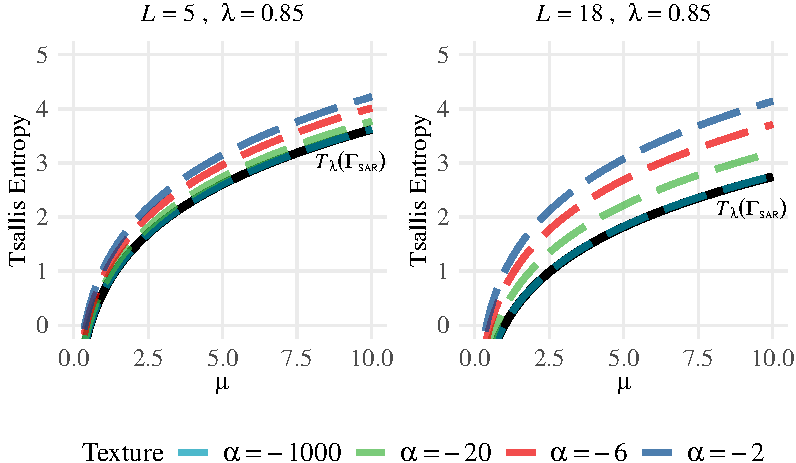
\includegraphics[keepaspectratio]{Figures-R1/fig-tsallis-convergence_L18-1.pdf}}

}

\caption{\label{fig-tsallis-convergence_L18}Tsallis entropy
\(T_{\lambda}(\mathcal{G}^0_I(\alpha, \mu, L))\) converges to
\(T_{\lambda}(\Gamma_{\mathrm{SAR}}(\mu, L))\) as \(\alpha\) decreases.}

\end{figure}%

For the highly heterogeneous case (\(\alpha=-2\)), entropy values are
very similar for \(L=5\) and \(L=18\), since texture dominates over
speckle. In contrast, in the homogeneous limit (\(\alpha \to -\infty\)),
texture effects vanish and the entropy is mainly determined by speckle.
With a low number of looks, speckle is strong and increases the
uncertainty, which raises the entropy values. However, the curves for
different \(\alpha\) values appear more concentrated, since the
contribution of texture to entropy is masked by the dominant speckle. As
the number of looks increases, speckle is progressively reduced and
entropy decreases. This reduction of speckle makes the \DIFdelbegin \DIFdel{entropy excess
\(\Delta_\alpha\) }\DIFdelend \DIFaddbegin \DIFadd{texture-induced
contribution \(\Delta_\lambda(\alpha,\mu,L)\) }\DIFaddend more evident, resulting in
more separated curves across the values of \(\alpha\).

\subsection{Nonparametric Estimation of the Tsallis
Entropy}\label{nonparametric-estimation-of-the-tsallis-entropy}

\label{subsec:tsallis-np}

Following the spacing-based approach of
Vasicek~\citeproc{ref-vasicek1976test}{{[}30{]}} and Ebrahimi et
al.~\citeproc{ref-Ebrahimi1994}{{[}31{]}} for the Shannon entropy, and
the methodology for the Rényi entropy proposed by Al-Labadi et
al.~\citeproc{ref-AlLabadi2024}{{[}32{]}}, we derive a nonparametric
estimator for the Tsallis entropy.

Let \(Q(p)=F^{-1}(p)\) denote the quantile function for \(p\in(0,1)\),
where \(F(z)\) is the cumulative distribution function of the continuous
random variable \(Z\). From~\eqref{eq:tsallis}, the inner integral can
be expressed as an expectation under a random variable \(Z\) with pdf
\(f(z)\): \[
\int_{\mathcal B} f(z)^\lambda\,\mathrm{d}z
=\int_{\mathcal B} f(z)^{\lambda-1} f(z)\,\mathrm{d}z
=\mathbb{E}\!\left[f(Z)^{\lambda-1}\right].
\] Using the change of variables \(p=F(z)\) (hence
\(\mathrm{d}p=f(z)\,\mathrm{d}z\)) and the identity \(f(Q(p))=1/Q'(p)\),
we obtain \[
  \mathbb{E}\!\left[f(Z)^{\lambda-1}\right]
  = \int_{0}^{1} \bigl[Q'(p)\bigr]^{1-\lambda}\,\mathrm{d}p,
\] which yields the representation \begin{equation}
  T_\lambda(Z)
  =\frac{1}{\lambda-1}
     \left\{
       1-\int_{0}^{1}\bigl[Q'(p)\bigr]^{1-\lambda}\,\mathrm{d}p
     \right\}.
  \label{eq:Tsallis-quantile}
\end{equation} Let \(\bm{Z}=(Z_1,Z_2,\dots,Z_n)\) be an \(n\)-points
vector of independent and identically distributed random variables from
\(Z\sim \mathcal{D}\) with order statistics
\(Z_{(1)}\le Z_{(2)} \le \cdots\le Z_{(n)}\). The \(m\)-spacing, with
\(m\in\{1,2,\dots,\lfloor (n-1)/2\rfloor\}\), is \[
D_{i,m}:=Z_{(i+m)}-Z_{(i-m)},\qquad \text{for }\, i=1,2,\dots,n,
\] with boundary conventions \(Z_{(i-m)}:=Z_{(1)}\) if \(i\le m\) and
\(Z_{(i+m)}:=Z_{(n)}\) if \(i\ge n-m\), where \(\lfloor \cdot \rfloor\)
denotes the floor function. The \(m\)-spacing density estimator at
\(Z_{(i)}\) is \begin{equation}
\widehat f_n\bigl(Z_{(i)}\bigr)
=\frac{(m/n) \, c_i}{D_{i,m}}\,,\qquad \text{for } \,i=1,2,\dots,n,
\label{eq:density-spacing}
\end{equation} where \[
c_i=
\begin{cases}
\dfrac{m+i-1}{m} & \text{if } \; 1\le i\le m,\\[6pt]
2 & \text{if } \; m+1\le i\le n-m,\\[6pt]
\dfrac{n+m-i}{m} & \text{if } \; n-m+1\le i\le n.
\end{cases}
\] By construction, \(\widehat f_n(Z_{(i)})\approx f(Z_{(i)})\). Since
\(f(Q(p))\,Q'(p)=1\), taking the reciprocal yields an estimator of the
quantile derivative: \begin{equation}
\widehat{Q'}(p_i)
\;=\; \frac{1}{\widehat f_n(Z_{(i)})}
\;=\; \frac{D_{i,m}}{(m/n)\, c_i}\,,
\qquad \text{for } \, p_i \in (0,1).
\label{eq:Qprime-hat}
\end{equation} Approximating the integral in~\eqref{eq:Tsallis-quantile}
by a Riemann sum over the grid \(p_i=i/n\), for \(i=1,2,\dots, n\), and
inserting \(\widehat{Q'}(p_i)\) from~\eqref{eq:Qprime-hat} yields the
nonparametric Tsallis entropy estimator: \begin{align}
  \widehat T_{\lambda}(\bm{Z})
  &=\frac{1}{\lambda-1}\left\{
1-\frac{1}{n}\sum_{i=1}^{n}\bigl[\widehat{Q'}(p_i)\bigr]^{\,1-\lambda}
\right\} \nonumber\\[4pt]
  &= \frac{1}{\lambda-1}
  \left\{
    1-\frac{1}{n}
       \sum_{i=1}^{n}
       \left(
         \frac{D_{i,m}}{(m/n) \, c_i}
       \right)^{1-\lambda}
  \right\}.
  \label{eq:Tsallis-spacing-estimator}
\end{align} As \(\lambda \to 1\), \(T_\lambda\) converges to the Shannon
entropy and \(\widehat T_{\lambda}\) recovers the Vasicek
estimator~\citeproc{ref-vasicek1976test}{{[}30{]}}. While a formal proof
of consistency is not provided here, the estimator follows the same
\(m\)-spacing construction used for the Shannon
entropy~\citeproc{ref-vasicek1976test}{{[}30{]}},
\citeproc{ref-Ebrahimi1994}{{[}31{]}} and for the Rényi
entropy~\citeproc{ref-AlLabadi2024}{{[}32{]}}. Empirically,
\(\widehat T_\lambda\) exhibits the expected large-sample behavior
when~\(m,n\to\infty\) and \(m/n\to 0\). We use the heuristic spacing
formula \(m = \lfloor \sqrt{n} + 0.5 \rfloor\) proposed in
Ref.~\citeproc{ref-Crzcgorzewski1999}{{[}33{]}}.

\section{PROPOSED METHODOLOGY}\label{sec:met}

In this section, we first discuss the optimal value for the parameter
\(\lambda\) that is required for the Tsallis entropy, as well as a
correction for its estimation using the nonparametric entropy estimator.
These are preliminary steps toward the test statistic, which forms the
core of the proposed methodology. Next, we present the test statistic
and examine its behavior through a size and power analysis. Besides, we
describe the procedure of including an adaptive window scheme.

\subsection{\texorpdfstring{Optimal \(\lambda\)
value}{Optimal \textbackslash lambda value}}\label{sec-lambda}

We investigate the optimal order \(\lambda\) for the Tsallis entropy
estimator using simulated samples of size \(n = 49\) drawn from the
\(\Gamma_{\mathrm{SAR}}(1,5)\) model. The bias and mean squared error
(MSE) were evaluated for varying values of \(\lambda\) through a Monte
Carlo experiment.

As shown in Figure~\ref{fig-optimal_order-tsallis}, for the case
\(L=5\), the value \(\lambda = 0.85\) yields the lowest MSE while
maintaining a nearly zero bias. This behavior is consistent with what we
observed for other values of \(L>1\) and for larger sample sizes, such
as \(n=81\) and \(n=121\), where \(\lambda = 0.85\) also provides a good
balance between bias and MSE. For the particular case \(L=1\), the
optimal value is \(\lambda = 1.2\), which offers the best MSE--bias
trade-off.

\begin{figure}[hbt]

\centering{

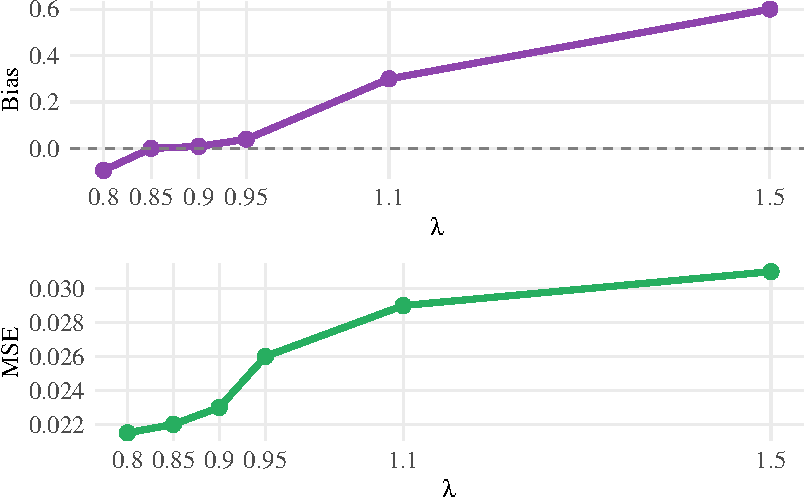
\includegraphics[width=0.9\linewidth,height=\textheight,keepaspectratio]{Figures-R1/fig-optimal_order-tsallis-1.pdf}

}

\caption{\label{fig-optimal_order-tsallis}Bias and MSE as a function of
\(\lambda\), for the Tsallis entropy estimator, with \(n = 49\),
\(\mu = 1\), and \(L = 5\).}

\end{figure}%

There is an interpretation for this optimal value of \(\lambda\). When
considering discrete probabilities, smaller values of this entropic
index amplify the effect of ``small'' probabilities on the total Tsallis
entropy. The \(\mathcal G^0\) and gamma distributions differentiate
mostly on their tails, so enhancing the effect of the tails improves our
ability to tell one from the other.

\subsection{Bootstrap Correction for Entropy
Estimator}\label{bootstrap-correction-for-entropy-estimator}

Following Refs.~\citeproc{ref-Frery2024}{{[}22{]}},
\citeproc{ref-Alpala2025}{{[}23{]}},
\citeproc{ref-Alpala2024}{{[}34{]}}, we refine the nonparametric entropy
estimator \(\widehat{T}_{\lambda}\) defined
in~\eqref{eq:Tsallis-spacing-estimator} with a bootstrap procedure,
obtaining: \[
\widetilde{T}_{\lambda} = 2\widehat{T}_{\lambda}(\bm{Z}) - \frac{1}{B} \sum_{b=1}^{B} \widehat{T}_{\lambda}(\bm{Z}^{(b)}),
\] where \(B\) is the number of bootstrap replicas, and \(\bm{Z}^{(b)}\)
denotes the \(b\)-th resampled dataset obtained by drawing \(n\)
observations with replacement from \(\bm{Z}\).

A Monte Carlo study with \(1000\) replicas for each sample size
\(n \in \{9, 25, 49, 81, 121\}\) was conducted using samples from
\(\Gamma_{\mathrm{SAR}}(1,5)\). The choice of \(L=5\) and \(\mu=1\)
(physically accepted) is illustrative and corresponds to the case
\(L>1\). For these values, the estimator performs properly with
\(\lambda=0.85\), and the bootstrap-corrected estimator
\(\widetilde{T}_{\lambda}\) with \(B=200\) reduces both bias and MSE
compared with the original estimator \(\widehat{T}_{\lambda}\), as shown
in Figure~\ref{fig-bias_mse_Tsallis}.

For the case \(L=1\), the estimator also performs properly when using
the bootstrap correction with \(\lambda=1.2\).

\begin{figure}[hbt]

\centering{

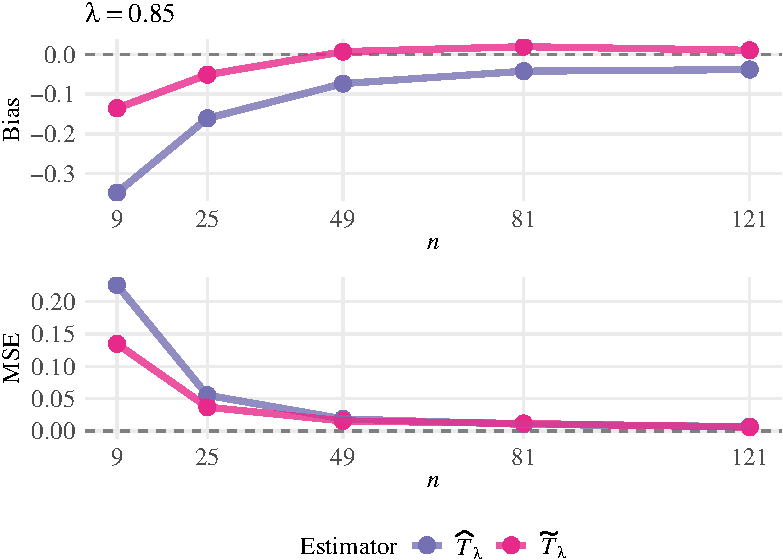
\includegraphics[width=0.9\linewidth,height=\textheight,keepaspectratio]{Figures-R1/fig-bias_mse_Tsallis-1.pdf}

}

\caption{\label{fig-bias_mse_Tsallis}Bias and MSE for the Tsallis
entropy estimators at the \(\Gamma_\text{SAR}(1,5)\) case.}

\end{figure}%

Heterogeneous samples occur when the window spans two or more different
areas, e.g., across an edge. They produce outliers that may have a
detrimental effect in resampling techniques. In Sec.~\ref{sec:adaptive}
we use adaptive windows to discard samples which are in disagreement
with the observations around the center pixel. Such trimming may reach
almost \SI{80}{\percent} of the observations when reducing from a window
of size \(11\times11\) pixels to another of size \(5\times5\) pixels.

\subsection{Hypothesis Testing}\label{hypothesis-testing}

We test whether the observed data come from a homogeneous
(\(\Gamma_{\mathrm{SAR}}(\mu, L)\)-distributed random variables) or a
heterogeneous (with underlying \(\mathcal{G}^0_I(\alpha, \mu, L)\) law)
region, as follows: \begin{equation}\label{eq:hypothesis_test}
\begin{cases}
\mathcal{H}_0: \mathbb{E}[\widetilde{T}_{\lambda}] = T_{\lambda}\bigl(\Gamma_{\mathrm{SAR}}(\mu,L)\bigr) & \text{(Homogeneous region)}, \\[6pt]
\mathcal{H}_1: \mathbb{E}[\widetilde{T}_{\lambda}] = T_{\lambda}\bigl(\mathcal{G}^0_I(\alpha, \mu, L)\bigr) & \text{(Heterogeneous region)}.
\end{cases}
\end{equation} Under \(\mathcal{H}_0\), the expected value of the
entropy estimator should match the theoretical
\(T_{\lambda}\bigl(\Gamma_{\mathrm{SAR}}(\mu,L)\bigr)\). Significant
deviations indicate heterogeneity.

\subsection{The Proposed Test}\label{the-proposed-test}

We propose a test statistic that identifies the discrepancy between
estimated and fitted theoretical entropy under homogeneity. Since the
number of looks \(L\geq1\) is known, we define the test statistic under
\(\mathcal{H}_0\) as follows: \begin{multline}
\label{eq-test-tsallis}
S_{\widetilde{T}_{\lambda}}(\bm{Z}; L) = \widetilde{T}_{\lambda} - \biggl\{ \frac{1}{\lambda - 1} \Bigl[ 1 -
\exp\Bigl(
(1 - \lambda)\ln \widehat{\mu}\\
+ (\lambda - 1)\ln L
+ \ln\Gamma\bigl(\lambda(L - 1) + 1\bigr) \\
- \lambda\ln\Gamma(L)
- \bigl(\lambda(L - 1) + 1\bigr)\ln \lambda
\Bigr) \Bigr] \biggr\},
\end{multline} where \(\widehat{\mu} = \frac{1}{n} \sum_{i=1}^n Z_i\) is
the sample mean. This test statistic can be interpreted as \[
S_{\widetilde T_\lambda} 
= 
\underbrace{\widetilde T_\lambda}_{\text{estimated}} 
\;-\;
\underbrace{T_\lambda\bigl(\Gamma_{\mathrm{SAR}}(\widehat{\mu},L)\bigr)}_{\text{fitted theoretical entropy,  under } \mathcal{H}_0}\hspace{-1.5em},
\] i.e., \(S_{\widetilde T_\lambda}\) is the difference between the
model-free estimated entropy and the fitted value under homogeneity.
Values close to zero indicate that the region behaves like
fully-developed speckle, while large positive values signal entropy
excess, hence heterogeneity. This formulation avoids the need to
estimate the \(\mathcal{G}^0_I\) parameter \(\alpha\), offering a
simple, interpretable, and statistically grounded test. Moreover, the
proposed method remains effective for small samples, aided by the
bootstrap bias correction. It is important to note that the unrestricted
test statistic is given by \[
\widetilde{T}_\lambda - T_\lambda(\mathcal{G}^0_I(\widehat{\alpha}, \widehat{\mu}, L)),
\] which is used in the power study.

Figure~\ref{fig-densities-tsallis6} shows the empirical distribution of
\(S_{\widetilde{T}_{\lambda}}\) under \(\mathcal{H}_0\), obtained from
\(10^4\) Monte Carlo simulations with different sample sizes
\(n \in \{25, 49, 81,121\}\), \(\lambda = 0.85\), and
\(L \in \{5,18\}\). The empirical densities are tightly concentrated
around zero, confirming that under \(\mathcal{H}_0\), the test
statistics have mean approximately \(0\); at the same time, their
moderately heavy tails reveal sensitivity to departures from
homogeneity, which is desirable for detecting subtle textures.

\begin{figure}[hbt]

\centering{

\pandocbounded{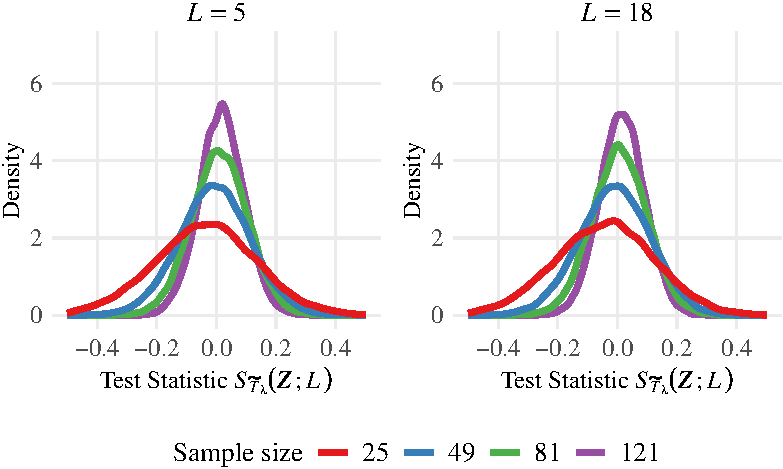
\includegraphics[keepaspectratio]{Figures-R1/fig-densities-tsallis6-1.pdf}}

}

\caption{\label{fig-densities-tsallis6}Empirical densities obtained by
means of Monte Carlo simulations of
\(S_{\widetilde{T}_{\lambda}}(\bm{Z}; L)\) under \(\mathcal{H}_0\), with
\(\lambda=0.85\).}

\end{figure}%

Under the asymptotic properties of the entropy
estimators~\citeproc{ref-vasicek1976test}{{[}30{]}},
\citeproc{ref-VanEs1992}{{[}35{]}}, for sufficiently large samples,
\(S_{\widetilde T_\lambda}(\bm{Z};L)\) follows an asymptotic Normal
distribution, \emph{i.e.}, the following convergence in distribution
holds: \[
  S_{\widetilde T_\lambda}(\bm Z;L)\;
  \overset{\mathcal{D}}{\underset{n \to \infty}{\longrightarrow}}\;
  \mathcal N\!\bigl(\mu_S,\sigma_S^{2}\bigr),
\] where \(\xrightarrow[n\rightarrow\infty]{\mathcal{D}}\) denotes the
distribution convergence,
\(\mu_S = \mathbb{E}[S_{\widetilde T_\lambda}(\bm{Z};L)]\) and
\(\sigma^2_S = \mathrm{Var}[S_{\widetilde T_\lambda}(\bm{Z};L)]\) are
the theoretical mean and variance of the test statistic under
\(\mathcal{H}_0\), respectively. This asymptotic normality can be
explained by noting that the entropy estimator (and hence
\(S_{\widetilde T_\lambda}\)) can be expressed as a sum or average of
numerous observations; therefore, by the Central Limit Theorem and the
Delta Method
(see~\citeproc{ref-MathematicalStatisticsvII2015}{{[}36{]}}, Ch. 7), its
sampling distribution approaches a Gaussian form for large \(n\). In
practice, we estimate \(\widehat{\mu}_S\) and \(\widehat{\sigma}_S\) via
Monte Carlo under \(\mathcal{H}_0\). Therefore, \begin{equation*}
\varepsilon = \frac{{S_{\widetilde T_\lambda}(\bm{Z}; L) - \widehat{\mu}_S}}{{\widehat{\sigma}_S}}
\end{equation*} is asymptotically standard Normal distributed for large
\(n\). Consequently, two-sided \(p\)-values were obtained as
\(2\Phi(-|\varepsilon|)\), where \(\Phi(\cdot)\) is the cumulative
distribution function of the standard Normal distribution.

The practical procedure is as follows: first, compute the test statistic
\(S_{\widetilde T_\lambda}(\bm{Z}; L)\) for the observed data; then,
standardize it using the estimated mean \(\widehat{\mu}_S\) and the
standard deviation \(\widehat{\sigma}_S\); next, compute the \(p\)-value
as \(2\Phi(-|\varepsilon|)\); and finally, make a decision by comparing
the \(p\)-value with a threshold value, e.g., \(0.05\). The
corresponding workflow is illustrated by the block diagram in
Figure~\ref{fig:entropy-diagram-test}.

\begin{figure}[hbt]
    \centering
\begin{tikzpicture}[
  node distance=1.5cm and 1.5cm,
  box/.style={
    rectangle, draw=black, fill=teal!20,
    minimum width=3.5cm, minimum height=1.2cm,
    align=center, font=\small, text=black, font=\bfseries
  },
  arrow/.style={
    -{Stealth[length=2mm, width=1.2mm]},
    semithick
  }
]
  % 
  \node[box] (raw) {1. Calculate\\test statistic\\ $S(\bm{Z})$};
  \node[box,right=of raw] (std) {2. Standardize\\test statistic\\ $\varepsilon=(S-\hat\mu_S)/\hat\sigma_S$};

  % 
  \node[box,below=of raw] (pval) {4. Make decision \\ Reject $\mathcal{H}_0$ if \\ $p\text{-value} <0.05$};
  \node[box,right=of pval] (dec) {3. Compute \\ $p$-value \\ $2\Phi(-|\varepsilon|)$};

  % 
  \draw[arrow] (raw.east) -- (std.west);
  \draw[arrow] (std.south) -- (dec.north);   
  \draw[arrow] (dec.west) -- (pval.east);    
 % \draw[arrow] (pval.north) -- (raw.south);  
\end{tikzpicture}
    \caption{Workflow of the entropy‐based hypothesis test.}
    \label{fig:entropy-diagram-test}
\end{figure}

The \(p\)-value quantifies the evidence against the null hypothesis of
homogeneity (fully developed speckle under the \(\Gamma_{\text{SAR}}\)
model). High values (e.g., \(p>0.05\)) will be interpreted as no
significant deviation from homogeneity, whereas low \(p\)-values (e.g.,
\(p<0.05\)) will be taken as evidence of heterogeneity. These
\(p\)-values are later visualized as maps in Section~\ref{sec:app},
enabling a spatial interpretation of the detected departures from
homogeneity.

\subsection{Size and Power Analysis of the Proposed
Test}\label{size-and-power-analysis-of-the-proposed-test}

The statistical validity and effectiveness of the proposed Tsallis
entropy--based test was examined through two fundamental properties:
test size (or false alarm, Type~I error) and test power (detection
probability, one minus Type~II error). These provide insight into the
probability of incorrect decisions in hypothesis testing.

The size of a statistical test, also known as the Type~I~error rate,
refers to the probability of incorrectly rejecting the null hypothesis
\(\mathcal{H}_0\) when it is in fact true. In hypothesis testing,
practitioners typically specify a nominal significance level, commonly
set at \SI{1}{\percent}, \SI{5}{\percent}, or \SI{10}{\percent}, which
represents acceptable probabilities of committing a Type~I~error. A
well-calibrated test should reproduce these levels empirically across
sample sizes and conditions. To assess this, we performed \(1000\) Monte
Carlo replications under \(\mathcal{H}_0\) with data from the
\(\Gamma_{\mathrm{SAR}}(1,L)\) distribution, computing the test
statistic via a bootstrap entropy estimator using \(B=100\) and
\(\lambda=0.85\). The empirical size was then estimated as the
proportion of replications in which the null hypothesis was incorrectly
rejected. The observed Type~I~error rates remained close to the nominal
levels, confirming the validity and proper calibration of the proposed
procedures.

The power of a test is its probability of correctly rejecting
\(\mathcal{H}_0\) when it is false. Equivalently, it equals \(1-\beta\),
where \(\beta\) is the Type~II~error rate. High power thus indicates
strong sensitivity to departures from \(\mathcal{H}_0\). To assess
power, we simulated data under the alternative hypothesis
\(\mathcal{H}_1\), assuming a \(\mathcal{G}^0_I(-2,1,L)\) distribution.
Again, \(1000\) Monte Carlo replications were performed for each
configuration of sample size \(n \in \{25, 49, 81, 121\}\) and
\(L \in \{5, 8, 18\}\), and the test statistic was computed using the
bootstrap estimator with \(B=100\) and \(\lambda=0.85\). As expected,
power increases with both the sample size and the number of looks,
confirming the effectiveness of the Tsallis entropy--based test in
detecting departures from the null hypothesis.

The complete results for both size and power are reported in
Table~\ref{tab:size-power-tsallis}.

\renewcommand{\arraystretch}{1}

\begin{table}[hbt]
\centering
\DIFdelbeginFL %DIFDELCMD < \centering
%DIFDELCMD < %%%
\DIFdelendFL \caption{\label{tab:size-power-tsallis}Size and Power of the $S_{\widetilde{T}_{\lambda}}(\bm{Z})$ test statistic.}
\DIFdelbeginFL %DIFDELCMD < \resizebox{\ifdim\width>\linewidth\linewidth\else\width\fi}{!}{
%DIFDELCMD < \fontsize{10}{12}\selectfont
%DIFDELCMD < \begin{tabu} to \linewidth {>{\raggedleft}X>{\raggedleft}X>{\centering}X>{\centering}X>{\centering}X>{\centering}X>{\centering}X>{\centering}X}
%DIFDELCMD < \toprule
%DIFDELCMD < \multicolumn{2}{c}{ } & \multicolumn{3}{c}{Size} & \multicolumn{3}{c}{Power} \\
%DIFDELCMD < \cmidrule(l{3pt}r{3pt}){3-5} \cmidrule(l{3pt}r{3pt}){6-8}
%DIFDELCMD < \multicolumn{1}{c}{$\bm{L}$} & \multicolumn{1}{c}{$\bm{n}$} & \multicolumn{1}{c}{$\hphantom{00}\SI{1}{\percent}$} & \multicolumn{1}{c}{$\hphantom{00}\SI{5}{\percent}$} & \multicolumn{1}{c}{$\hphantom{00}\SI{10}{\percent}$} & \multicolumn{1}{c}{$\hphantom{00}\SI{1}{\percent}$} & \multicolumn{1}{c}{$\hphantom{00}\SI{5}{\percent}$} & \multicolumn{1}{c}{$\hphantom{00}\SI{10}{\percent}$}\\
%DIFDELCMD < \midrule
%DIFDELCMD <  & 25 & $\phantom{-}0.014$ & $\phantom{-}0.051$ & $\phantom{-}0.103$ & $\phantom{-}0.958$ & $\phantom{-}0.991$ & $\phantom{-}0.990$\\
%DIFDELCMD < 

%DIFDELCMD <  & 49 & $\phantom{-}0.011$ & $\phantom{-}0.048$ & $\phantom{-}0.107$ & $\phantom{-}0.990$ & $\phantom{-}1.000$ & $\phantom{-}0.999$\\
%DIFDELCMD < 

%DIFDELCMD <  & 81 & $\phantom{-}0.012$ & $\phantom{-}0.057$ & $\phantom{-}0.101$ & $\phantom{-}0.997$ & $\phantom{-}0.998$ & $\phantom{-}0.999$\\
%DIFDELCMD < 

%DIFDELCMD < \multirow{-4}{*}[1.5\dimexpr\aboverulesep+\belowrulesep+\cmidrulewidth]{\raggedleft\arraybackslash 5} & 121 & $\phantom{-}0.014$ & $\phantom{-}0.060$ & $\phantom{-}0.116$ & $\phantom{-}0.999$ & $\phantom{-}0.999$ & $\phantom{-}0.997$\\
%DIFDELCMD < \cmidrule{1-8}
%DIFDELCMD <  & 25 & $\phantom{-}0.010$ & $\phantom{-}0.049$ & $\phantom{-}0.108$ & $\phantom{-}0.992$ & $\phantom{-}1.000$ & $\phantom{-}1.000$\\
%DIFDELCMD < 

%DIFDELCMD <  & 49 & $\phantom{-}0.008$ & $\phantom{-}0.055$ & $\phantom{-}0.108$ & $\phantom{-}1.000$ & $\phantom{-}0.999$ & $\phantom{-}1.000$\\
%DIFDELCMD < 

%DIFDELCMD <  & 81 & $\phantom{-}0.012$ & $\phantom{-}0.052$ & $\phantom{-}0.097$ & $\phantom{-}0.998$ & $\phantom{-}1.000$ & $\phantom{-}0.999$\\
%DIFDELCMD < 

%DIFDELCMD < \multirow{-4}{*}[1.5\dimexpr\aboverulesep+\belowrulesep+\cmidrulewidth]{\raggedleft\arraybackslash 8} & 121 & $\phantom{-}0.016$ & $\phantom{-}0.072$ & $\phantom{-}0.116$ & $\phantom{-}0.998$ & $\phantom{-}1.000$ & $\phantom{-}0.999$\\
%DIFDELCMD < \cmidrule{1-8}
%DIFDELCMD <  & 25 & $\phantom{-}0.015$ & $\phantom{-}0.052$ & $\phantom{-}0.111$ & $\phantom{-}1.000$ & $\phantom{-}1.000$ & $\phantom{-}1.000$\\
%DIFDELCMD < 

%DIFDELCMD <  & 49 & $\phantom{-}0.013$ & $\phantom{-}0.046$ & $\phantom{-}0.099$ & $\phantom{-}1.000$ & $\phantom{-}1.000$ & $\phantom{-}1.000$\\
%DIFDELCMD < 

%DIFDELCMD <  & 81 & $\phantom{-}0.013$ & $\phantom{-}0.047$ & $\phantom{-}0.105$ & $\phantom{-}1.000$ & $\phantom{-}1.000$ & $\phantom{-}1.000$\\
%DIFDELCMD < 

%DIFDELCMD < \multirow{-4}{*}[1.5\dimexpr\aboverulesep+\belowrulesep+\cmidrulewidth]{\raggedleft\arraybackslash 18} & 121 & $\phantom{-}0.012$ & $\phantom{-}0.065$ & $\phantom{-}0.109$ & $\phantom{-}1.000$ & $\phantom{-}1.000$ & $\phantom{-}1.000$\\
%DIFDELCMD < \bottomrule
%DIFDELCMD < \end{tabu}}
%DIFDELCMD < %%%
\DIFdelendFL \DIFaddbeginFL \resizebox{\ifdim\width>\linewidth\linewidth\else\width\fi}{!}{
\fontsize{10}{12}\selectfont
\begin{tabular}[t]{rrcccccc}
\toprule
\multicolumn{2}{c}{ } & \multicolumn{3}{c}{Size} & \multicolumn{3}{c}{Power} \\
\cmidrule(l{3pt}r{3pt}){3-5} \cmidrule(l{3pt}r{3pt}){6-8}
\multicolumn{1}{c}{$\bm{L}$} & \multicolumn{1}{c}{$\bm{n}$} & \multicolumn{1}{c}{$\hphantom{00}\SI{1}{\percent}$} & \multicolumn{1}{c}{$\hphantom{00}\SI{5}{\percent}$} & \multicolumn{1}{c}{$\hphantom{00}\SI{10}{\percent}$} & \multicolumn{1}{c}{$\hphantom{00}\SI{1}{\percent}$} & \multicolumn{1}{c}{$\hphantom{00}\SI{5}{\percent}$} & \multicolumn{1}{c}{$\hphantom{00}\SI{10}{\percent}$}\\
\midrule
 & 25 & $\phantom{-}0.014$ & $\phantom{-}0.051$ & $\phantom{-}0.103$ & $\phantom{-}0.958$ & $\phantom{-}0.991$ & $\phantom{-}0.990$\\

 & 49 & $\phantom{-}0.011$ & $\phantom{-}0.048$ & $\phantom{-}0.107$ & $\phantom{-}0.990$ & $\phantom{-}1.000$ & $\phantom{-}0.999$\\

 & 81 & $\phantom{-}0.012$ & $\phantom{-}0.057$ & $\phantom{-}0.101$ & $\phantom{-}0.997$ & $\phantom{-}0.998$ & $\phantom{-}0.999$\\

\multirow{-4}{*}[1.5\dimexpr\aboverulesep+\belowrulesep+\cmidrulewidth]{\raggedleft\arraybackslash 5} & 121 & $\phantom{-}0.014$ & $\phantom{-}0.060$ & $\phantom{-}0.116$ & $\phantom{-}0.999$ & $\phantom{-}0.999$ & $\phantom{-}0.997$\\
\cmidrule{1-8}
 & 25 & $\phantom{-}0.010$ & $\phantom{-}0.049$ & $\phantom{-}0.108$ & $\phantom{-}0.992$ & $\phantom{-}1.000$ & $\phantom{-}1.000$\\

 & 49 & $\phantom{-}0.008$ & $\phantom{-}0.055$ & $\phantom{-}0.108$ & $\phantom{-}1.000$ & $\phantom{-}0.999$ & $\phantom{-}1.000$\\

 & 81 & $\phantom{-}0.012$ & $\phantom{-}0.052$ & $\phantom{-}0.097$ & $\phantom{-}0.998$ & $\phantom{-}1.000$ & $\phantom{-}0.999$\\

\multirow{-4}{*}[1.5\dimexpr\aboverulesep+\belowrulesep+\cmidrulewidth]{\raggedleft\arraybackslash 8} & 121 & $\phantom{-}0.016$ & $\phantom{-}0.072$ & $\phantom{-}0.116$ & $\phantom{-}0.998$ & $\phantom{-}1.000$ & $\phantom{-}0.999$\\
\cmidrule{1-8}
 & 25 & $\phantom{-}0.015$ & $\phantom{-}0.052$ & $\phantom{-}0.111$ & $\phantom{-}1.000$ & $\phantom{-}1.000$ & $\phantom{-}1.000$\\

 & 49 & $\phantom{-}0.013$ & $\phantom{-}0.046$ & $\phantom{-}0.099$ & $\phantom{-}1.000$ & $\phantom{-}1.000$ & $\phantom{-}1.000$\\

 & 81 & $\phantom{-}0.013$ & $\phantom{-}0.047$ & $\phantom{-}0.105$ & $\phantom{-}1.000$ & $\phantom{-}1.000$ & $\phantom{-}1.000$\\

\multirow{-4}{*}[1.5\dimexpr\aboverulesep+\belowrulesep+\cmidrulewidth]{\raggedleft\arraybackslash 18} & 121 & $\phantom{-}0.012$ & $\phantom{-}0.065$ & $\phantom{-}0.109$ & $\phantom{-}1.000$ & $\phantom{-}1.000$ & $\phantom{-}1.000$\\
\bottomrule
\end{tabular}}
\DIFaddendFL \end{table}

\subsection{Adaptive Windows}\label{sec:adaptive}

When working on simulated or real images, the spatial context must be
taken into consideration, because each sample used to compute the test
statistic may overlap areas with different distributions. Intuitively,
the use of a different window size to compute the test statistics may be
crucial to avoid estimating values by using samples that belong to two,
even three or more different distributions.

Our approach builds on the adaptive windowing algorithm for SAR images
proposed by Park et al.~\citeproc{ref-Park1999}{{[}25{]}}, which adjusts
the analysis window size according to an estimate of the local
homogeneity of the scene. To this end, for each pixel \((i,j)\), let
\(w_{ij}\) be the window centered at \((i,j)\) with radius
\(N_{ij} \ge 1\), defined as: \begin{equation*}
w_{ij} = \{(i',j'),\, i-N_{ij} \le i' \le i+N_{ij} \,\wedge\, j-N_{ij} \le j' \le j+N_{ij}\}.
\end{equation*} Then, the border of this window is: \begin{multline*}
b_{ij} = \{(i',j') \in w_{ij},\, i' = i-N_{ij} \,\vee\, i' = i+N_{ij} \,\vee\\
j' = j-N_{ij} \,\vee\, j' = j+N_{ij}\}.
\end{multline*} The coefficient of variation is computed over the border
of the current window as: \begin{equation*}
C_{ij} = \frac{\sigma_{ij}}{\mu_{ij}},
\end{equation*} where the mean \(\mu_{ij}\) and the standard deviation
\(\sigma_{ij}\) are calculated using only the border pixels \(b_{ij}\)
of \(w_{ij}\).

For SAR intensity images (fully-developed speckle with \(L\) looks), the
coefficient of variation in homogeneous areas satisfies
\begin{equation*}
C_{ij} \approx \sigma_n := \frac{1}{\sqrt{L}}.
\end{equation*}

The homogeneity criterion is defined by comparing \(C_{ij}\) with an
adaptive threshold \(U_{ij}\) given by: \begin{equation*}
U_{ij} = \eta\!\left( 1 + \sqrt{\frac{1 + 2\sigma_n^2}{8\,(W_{ij} - 1)}} \right)\sigma_n,
\end{equation*} where \(W_{ij} = 2N_{ij} + 1\) is the current window
side length, and \(\eta\) is a tuning parameter controlling the degree
of smoothing. Values near \(\eta=1\) provide limited speckle
suppression, while larger values increase smoothing and yield stronger
noise reduction.

The window radius \(N_{ij}\) is updated dynamically and locally as
follows: \[
N_{ij}^{\text{updated}} =
\begin{cases}
\min\{N_{ij} + 1,\, N_{\max}\}, & \text{if } C_{ij} \leq U_{ij}, \\
\max\{N_{ij} - 1,\, N_{\min}\}, & \text{if } C_{ij} > U_{ij},
\end{cases}
\] where \(N_{\max}\) and \(N_{\min}\) denote the maximum and minimum
allowed window radius, respectively. Since \(W_{ij}=2N_{ij}+1\), these
bounds on the radius induce the corresponding minimum and maximum window
sides \(W_{\min}=2N_{\min}+1\) and \(W_{\max}=2N_{\max}+1\).

In homogeneous regions, where \(C_{ij}\leq U_{ij}\), the window radius
increases up to \(N_{\max}\), enhancing speckle reduction and
stabilizing the estimates. In heterogeneous regions, where
\(C_{ij}>U_{ij}\), the window radius decreases down to \(N_{\min}\),
preserving edges and preventing class mixing.

Once the window radius \(N_{ij}\) has been determined for pixel
\((i,j)\), the corresponding sample is extracted and the proposed test
in\DIFaddbegin \DIFadd{~}\DIFaddend \eqref{eq-test-tsallis} is applied to obtain a local test value. This
produces a map of \DIFaddbegin \DIFadd{test }\DIFaddend statistics over the image.

\DIFdelbegin \DIFdel{Because the final window size \(W_{ij}\) is selected from the data, the
null distribution of the adaptive statistic need not coincide exactly
with that of a fixed-window statistic. For this reason, the adaptive
case requires an additional null diagnostic and calibration analysis,
described next }\DIFdelend \DIFaddbegin \DIFadd{The behavior of this adaptive test statistic under \(\mathcal H_0\) is
examined in the next subsection}\DIFaddend .

\subsection{Test statistic behavior under the null hypothesis and
adaptive windows}\label{sec:adaptive-null}

Table~\ref{tab:size-power-tsallis} \DIFdelbegin \DIFdel{relates }\DIFdelend \DIFaddbegin \DIFadd{summarizes }\DIFaddend the behavior of the test
statistic under the null hypothesis for windows of fixed size. Since the
procedure is adaptive, the final window size \(W_{ij}\) \DIFdelbegin \DIFdel{at position
\((i,j)\) is selected from the data}\DIFdelend \DIFaddbegin \DIFadd{may vary across
pixels}\DIFaddend , and the \DIFdelbegin \DIFdel{test statistic behavior may be different. We verified that these distributions differ, and obtained
the \(p\)-values under
this realistic configuration}\DIFdelend \DIFaddbegin \DIFadd{behavior of the test statistic may differ from the
fixed-window case. We therefore examined the test statistic under
\(\mathcal H_0\) when the adaptive-window rule is used}\DIFaddend .

For this purpose, we generated an image of size \(1000\times1000\) under
\(\mathcal H_0\), i.e., with observations from iid
\(\Gamma_{\mathrm{SAR}}(10,16)\) random variables. We used
\(\lambda=0.85\), bootstrap size \(B=100\), and windows of size
\(W\in\{5,7,9,11\}\), with \(\eta=3\). We left a guard region of five
pixels and only applied the procedure to the interior region. This guard
region allows every pixel in the interior region to use the largest
possible window (\(11\times11\) pixels), if needed.

Table~\ref{tbl-null-calibration-adaptive} \DIFdelbegin \DIFdel{reports }\DIFdelend \DIFaddbegin \DIFadd{gives }\DIFaddend summary statistics
separately for each admissible window size \(W\): the mean
\(\mu_{\mathcal H_0}(W)\) and standard deviation
\(\sigma_{\mathcal H_0}(W)\). \DIFdelbegin \DIFdel{With these values, we corrected the empirical distribution }\DIFdelend \DIFaddbegin \DIFadd{These quantities summarize the behavior }\DIFaddend of
the test statistic \DIFdelbegin \DIFdel{, cf. ~\eqref{eq:standar},
and obtained }\DIFdelend \DIFaddbegin \DIFadd{under \(\mathcal H_0\) for the simulated homogeneous
image and the adaptive-window setting considered here.
}

\DIFadd{In the final }\DIFaddend \(p\)\DIFdelbegin \DIFdel{-values adjusted for the adaptive window scheme}\DIFdelend \DIFaddbegin \DIFadd{-value computation, the window-dependent mean
\(\mu_{\mathcal H_0}(W)\) is used to center the test statistic according
to the selected window size. The corresponding scale
\(\sigma_{\mathcal H_0}(W)\) is reported in the table, but it is not
used directly in the final standardization; instead,
Eq.~\eqref{eq:standar} uses the observed scale defined below}\DIFaddend .

\begin{table}

\caption{\label{tbl-null-calibration-adaptive}Empirical mean and standard deviation of the test statistic under the null 
hypothesis for each fixed window size.}

\centering{

\centering


\begin{tabular}{crr}
\toprule
$W$ & $\mu_{\mathcal H_0}(W)$ & $\sigma_{\mathcal H_0}(W)$ \\
\midrule
5  & $-0.063$  & $0.235$ \\
7  & $-0.012$  & $0.167$ \\
9  &  $0.010$ & $0.129$ \\
11 &  $0.022$ & $0.106$ \\
\bottomrule
\end{tabular}

}

\end{table}%

Figure~\ref{fig:null-diagnostic-adaptive} shows the empirical densities
of the test statistic under the null hypothesis for the four fixed
window sizes \(W\in\{5,7,9,11\}\) and for the adaptive procedure. Except
for the \(W=5\) case, the empirical densities look symmetric around
zero. The least spread case is \(W=11\), as expected because this is the
largest sample size. The distribution of the test statistic using the
adaptive procedure under \(\mathcal H_0\) is indistinguishable from the
\(W=11\) case, confirming that this adaptive approach behaves well under
the null hypothesis. Moreover, the adaptive method in this experiment
never selected windows of size \(W=5\).

\begin{figure}[hbt]
  \centering
  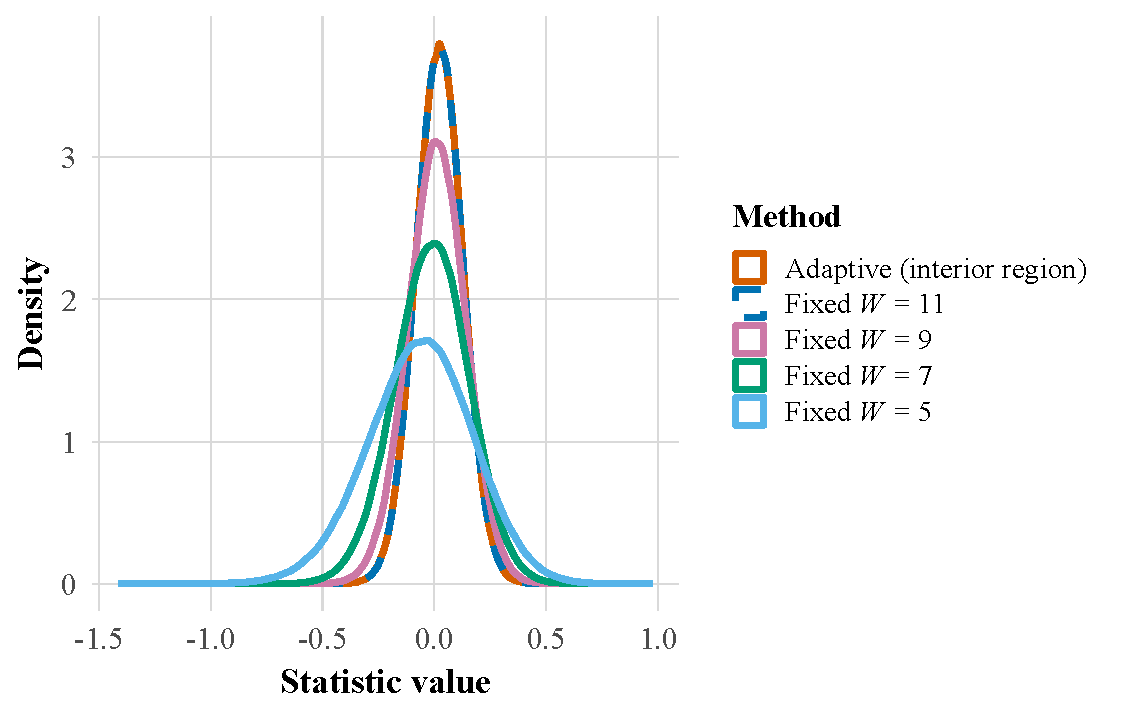
\includegraphics[width=0.98\columnwidth]{Figures-R1/distributions_statistic_density_1.pdf}
 \caption{Empirical densities of the test statistic under the null hypothesis and fixed and adaptive window sizes.}
  \label{fig:null-diagnostic-adaptive}
\end{figure}

\DIFdelbegin \DIFdel{After establishing the }\DIFdelend \DIFaddbegin \DIFadd{The \(p\)-values are computed pixelwise using empirical information
about the test statistic under the null hypothesis. This requires
estimates of the }\DIFaddend mean and standard deviation\DIFaddbegin \DIFadd{, that is, the location and
scale, }\DIFaddend of the test statistic under \DIFdelbegin \DIFdel{the null hypothesis and adaptive windows, the next step is to
convert the statistic field into \(p\)-values}\DIFdelend \DIFaddbegin \DIFadd{\(\mathcal H_0\). Since these
quantities may change with the window size in the adaptive procedure, we
estimated the window-dependent location \(\mu_{\mathcal H_0}(W)\)
separately for each admissible window size, \(W\in\{5,7,9,11\}\)}\DIFaddend .

\DIFdelbegin \DIFdel{Since }\DIFdelend \DIFaddbegin \DIFadd{The corresponding window-dependent scale }\DIFaddend \(\sigma_{\mathcal H_0}(W)\)
\DIFdelbegin \DIFdel{produces overly aggressive
standardization and excessive rejections}\DIFdelend \DIFaddbegin \DIFadd{was also estimated and reported in
Table~\ref{tbl-null-calibration-adaptive}. However, using this scale
directly to standardize the test-statistic values of real SAR scenes
produced excessive rejections in the \(p\)-value maps.
}

\DIFadd{This indicated that the scale obtained from the homogeneous simulation
was too small for the variability observed in real data. For this
reason}\DIFaddend , we used \DIFdelbegin \begin{displaymath}
\DIFdel{z_{ij}=\frac{S_{ij}-\mu_{\mathcal H_0}(W_{ij})}{\sigma_{\mathrm{obs}}},
%DIFDELCMD < \label{eq:standar}%%%
}\end{displaymath}%DIFAUXCMD
%DIFDELCMD <  %%%
\DIFdel{where }\DIFdelend \DIFaddbegin \DIFadd{a common observed scale, denoted by
}\DIFaddend \(\sigma_{\mathrm{obs}}\)\DIFdelbegin \DIFdel{is }\DIFdelend \DIFaddbegin \DIFadd{, computed as }\DIFaddend the empirical standard deviation
of the \DIFdelbegin \DIFdel{test statistic computed over all the pixels under
\(\mathcal H_0\) using adaptive windows.
In this way}\DIFdelend \DIFaddbegin \DIFadd{test-statistic values \(S_{ij}\) over the pixels of the image
under analysis.
}

\DIFadd{We used the following standardization: }\begin{equation}
\DIFadd{z_{ij}=
\frac{S_{ij}-\mu_{\mathcal H_0}(W_{ij})}{\sigma_{\mathrm{obs}}},
\label{eq:standar}
}\end{equation} \DIFadd{where \(S_{ij}\) is the test statistic at pixel \((i,j)\)
and \(W_{ij}\) is the final adaptive window selected at that pixel.
Thus}\DIFaddend , the procedure \DIFdelbegin \DIFdel{uses
window-dependent means and a scale better matched to the variability of the observed SAR data.Finally, the adaptive }\DIFdelend \DIFaddbegin \DIFadd{keeps the location under \(\mathcal H_0\) according
to the selected window size, while using a common empirical scale for
the processed scene.
}

\DIFadd{The adaptive }\DIFaddend \(p\)-values \DIFdelbegin \DIFdel{are computed
as }\DIFdelend \DIFaddbegin \DIFadd{are then computed as }\DIFaddend \[
p_{ij}=2\Phi\bigl(-|z_{ij}|\bigr).
\]

\DIFdelbegin \DIFdel{The same strategy was subsequently used in the comparative benchmark for the adaptive Shannon and }\DIFdelend \DIFaddbegin \DIFadd{To assess the behavior of the final adaptive \(p\)-values under
\(\mathcal H_0\), we computed the \(p\)-value map for the simulated
homogeneous image using the standardization in Eq.~\eqref{eq:standar}.
Figure~\ref{fig-null-pvalue-uniform} shows the histogram of the
resulting \(p\)-values, together with the density of the uniform
distribution \(\mathcal{U}[0,1]\). The histogram is approximately flat,
indicating that the adaptive \(p\)-values are consistent with the
expected behavior under \(\mathcal H_0\).
}

\begin{figure}[hbt]

\centering{

\pandocbounded{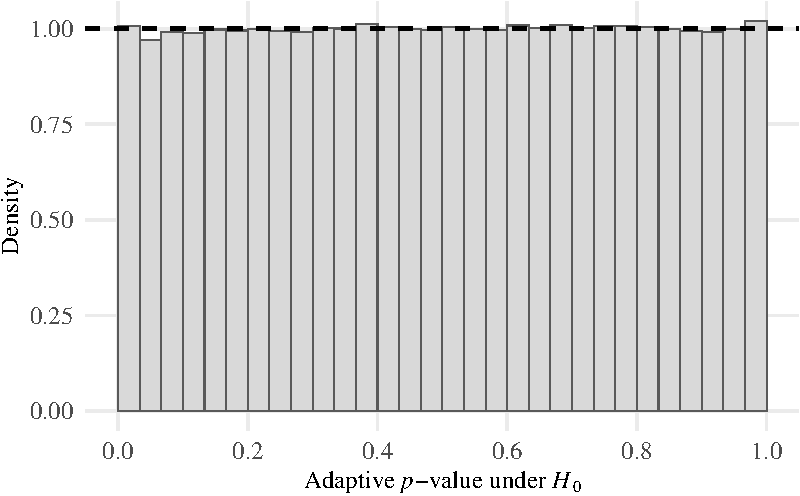
\includegraphics[keepaspectratio]{Figures-R1/fig-null-pvalue-uniform-1.pdf}}

}

\caption{\label{fig-null-pvalue-uniform}\DIFaddFL{Histogram of the adaptive
\(p\)-values under \(\mathcal H_0\) for the simulated homogeneous image.
The dashed line indicates the density of the uniform distribution
\(\mathcal{U}[0,1]\).}}

\end{figure}%DIF > 

\DIFadd{Table~\ref{tbl-null-pvalue-rejection} gives the empirical rejection
rates at the nominal levels \mbox{%DIFAUXCMD
\SI{1}{\percent}}\hskip0pt%DIFAUXCMD
, \mbox{%DIFAUXCMD
\SI{5}{\percent}}\hskip0pt%DIFAUXCMD
, and
\mbox{%DIFAUXCMD
\SI{10}{\percent}}\hskip0pt%DIFAUXCMD
. Each rate was computed as the proportion of valid
interior pixels whose adaptive \(p\)-value was smaller than the
corresponding nominal level. For the \(1000\times1000\) simulated image,
the valid region was defined by excluding the boundary margin associated
with the largest admissible adaptive window, \(W_{\max}=11\). This
corresponds to a margin of five pixels on each side, leaving
\(990\times990=980100\) valid interior pixels. These rates are close to
the corresponding nominal levels, supporting the behavior of the
proposed adaptive \(p\)-value computation.
}

\begin{table}[hbt]

\caption{\label{tbl-null-pvalue-rejection}\DIFaddFL{Empirical rejection rates of
the adaptive \(p\)-values under \(\mathcal H_0\) for the simulated
homogeneous image with \(L=16\), \(\eta=3\), \(\lambda=0.85\), and
adaptive windows.}}

\centering{

\centering\begingroup\fontsize{9}{11}\selectfont

\resizebox{\ifdim\width>\linewidth\linewidth\else\width\fi}{!}{
\begin{tabular}{ccc}
\toprule
\multicolumn{1}{c}{Nominal level} & \multicolumn{1}{c}{Empirical rejection rate} & \multicolumn{1}{c}{Valid pixels}\\
\midrule
\SI{1}{\percent} & 0.0106 & 980100\\
\SI{5}{\percent} & 0.0498 & 980100\\
\SI{10}{\percent} & 0.0990 & 980100\\
\bottomrule
\end{tabular}}
\endgroup{}

}

\end{table}%DIF > 

\DIFadd{Since the adaptive window rule depends on the number of looks \(L\) and
on the smoothing parameter \(\eta\), the quantities estimated under
\(\mathcal H_0\) must correspond to the same \((L,\eta)\) pair used to
process the image. \(L\) is determined by each SAR scene, whereas
\(\eta\) is the adaptive-window parameter evaluated in the analysis.
Therefore, the values reported in
Table~\ref{tbl-null-calibration-adaptive} should not be interpreted as
universal values for all scenes or all choices of \(\eta\). The settings
used for the real SAR scenes and for the comparative Shannon, }\DIFaddend Rényi\DIFdelbegin \DIFdel{entropy-based tests, }\DIFdelend \DIFaddbegin \DIFadd{, and
Tsallis benchmark are reported in the experimental section, }\DIFaddend as discussed
in \DIFdelbegin \DIFdel{Subsection~\ref{sec:entropy-benchmark}
.
}\DIFdelend \DIFaddbegin \DIFadd{Section~\ref{sec:entropy-benchmark}
}\DIFaddend 

\section{RESULTS}\label{sec:app}

In this section, we present the results obtained by applying the
proposed method to simulated data and actual SAR images.

\subsection{Analysis with Simulated Data}\label{sec-sim2}

Figure~\ref{fig:sim_scene} shows a simulated image of \(500\times500\)
pixels, generated from the structural design proposed by Gomez et
al.~\citeproc{ref-Gomez2017}{{[}37{]}} as a tool to assess the
performance of speckle-reduction filters. Each region is filled with
simulated samples drawn from the \(\mathcal{G}^0_I\) distribution
parametrized as in~\eqref{E:gi02}, considering different combinations of
the texture parameter \(\alpha\) and the mean \(\mu\), as indicated by
the labels in each quadrant of the image. Light regions correspond to
textured observations (heterogeneous), while darker regions represent
textureless areas (homogeneous).

\begin{figure}[hbt]
  \centering
  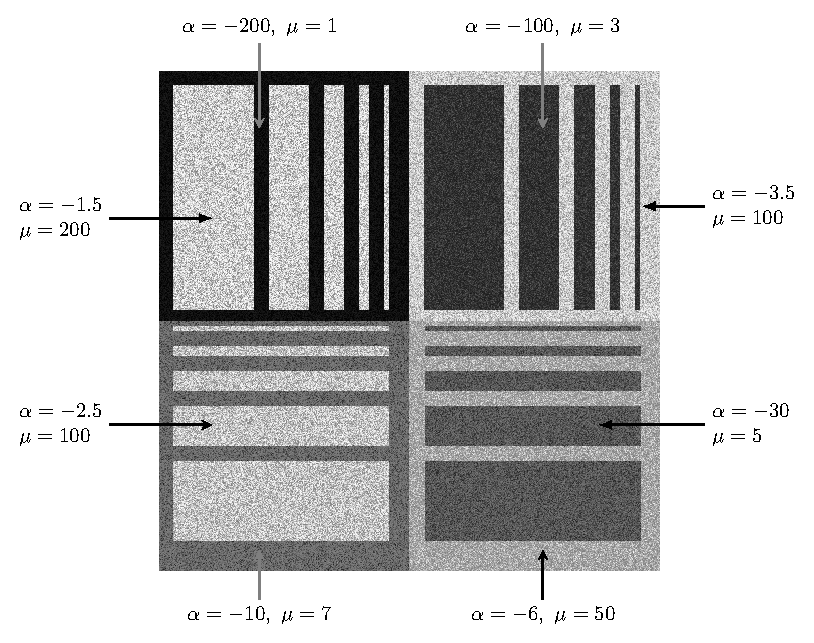
\includegraphics[width=0.9\columnwidth]{Figures/phantom_18.pdf}
  \caption{Simulated SAR intensity image ($L=18$).}
  \label{fig:sim_scene}
\end{figure}

The \(\alpha\) parameter of the \(\mathcal{G}_I^0\) distribution is
essential for interpreting texture characteristics. Values belonging to
\([-3, 0)\) suggest extremely textured targets, such as urban
zones~\citeproc{ref-Frery2019a}{{[}38{]}}. As the \(\alpha\) value
decreases, it indicates regions with moderate texture (in the
\([-6,-3)\) region), related to forest zones, while values below \(-6\)
correspond to textureless regions, such as pasture, agricultural fields,
and water bodies~\citeproc{ref-Neto2023}{{[}39{]}}.

The proposed Tsallis-based test statistic,
\(S_{\widetilde{T}_{\lambda}}\), was applied to the simulated image
using the adaptive windowing strategy with window sides ranging from
\(5\times5\) to \(11\times11\), i.e., \(N_{\min}=2\), \(N_{\max}=5\),
hence \(W_{\min}=5\) and \(W_{\max}=11\). For comparison, a fixed
\(7\times7\) window was also considered. For each window, \(B=100\)
bootstrap replications were performed to estimate the corrected test
statistic.

Figure~\ref{fig:simc1} shows the \(p\)-value map with the fixed window,
while Figures~\ref{fig:simc2}--\ref{fig:simc5} display the adaptive
results for \(\eta=1\), \(2\), \(3\), and \(4\). The corresponding
binary decision maps at a \(0.05\) significance level are shown in
Figures~\ref{fig:simbc1}--\ref{fig:simbc5}. We used a significance level
of \(0.05\) because it is a standard and practical threshold:
\(p\)-values below this value provide sufficient evidence to reject
local homogeneity without generating an excessive number of false
detections.

The colored representation provides an interpretable scale: dark red
regions (\(p \approx 0\)) indicate strong evidence of heterogeneity,
consistently appearing in highly textured zones, while dark blue regions
(\(p \approx 1\)) correspond to homogeneous areas. Intermediate colors
follow a smooth progression: orange \((p\in (0.2,0.4))\) denotes
transitional texture, whereas yellow--green to cyan \((p\in (0.4,0.8))\)
marks increasingly near-homogeneous areas.

Although the differences were subtle, the adaptive scheme exhibits the
expected behavior: larger windows in homogeneous areas provide smoother
estimates, while smaller windows in heterogeneous regions preserve
structural details.

\setlength{\dblfloatsep}{6pt}
\setlength{\dbltextfloatsep}{6pt}
\setlength{\textfloatsep}{6pt}
\captionsetup{font=footnotesize}
\captionsetup[sub]{aboveskip=2pt,belowskip=2pt}

\begin{figure*}[!t]
\centering
\captionsetup{font=footnotesize}
\captionsetup[sub]{aboveskip=2pt,belowskip=2pt}

\begin{subfigure}[t]{0.19\textwidth}
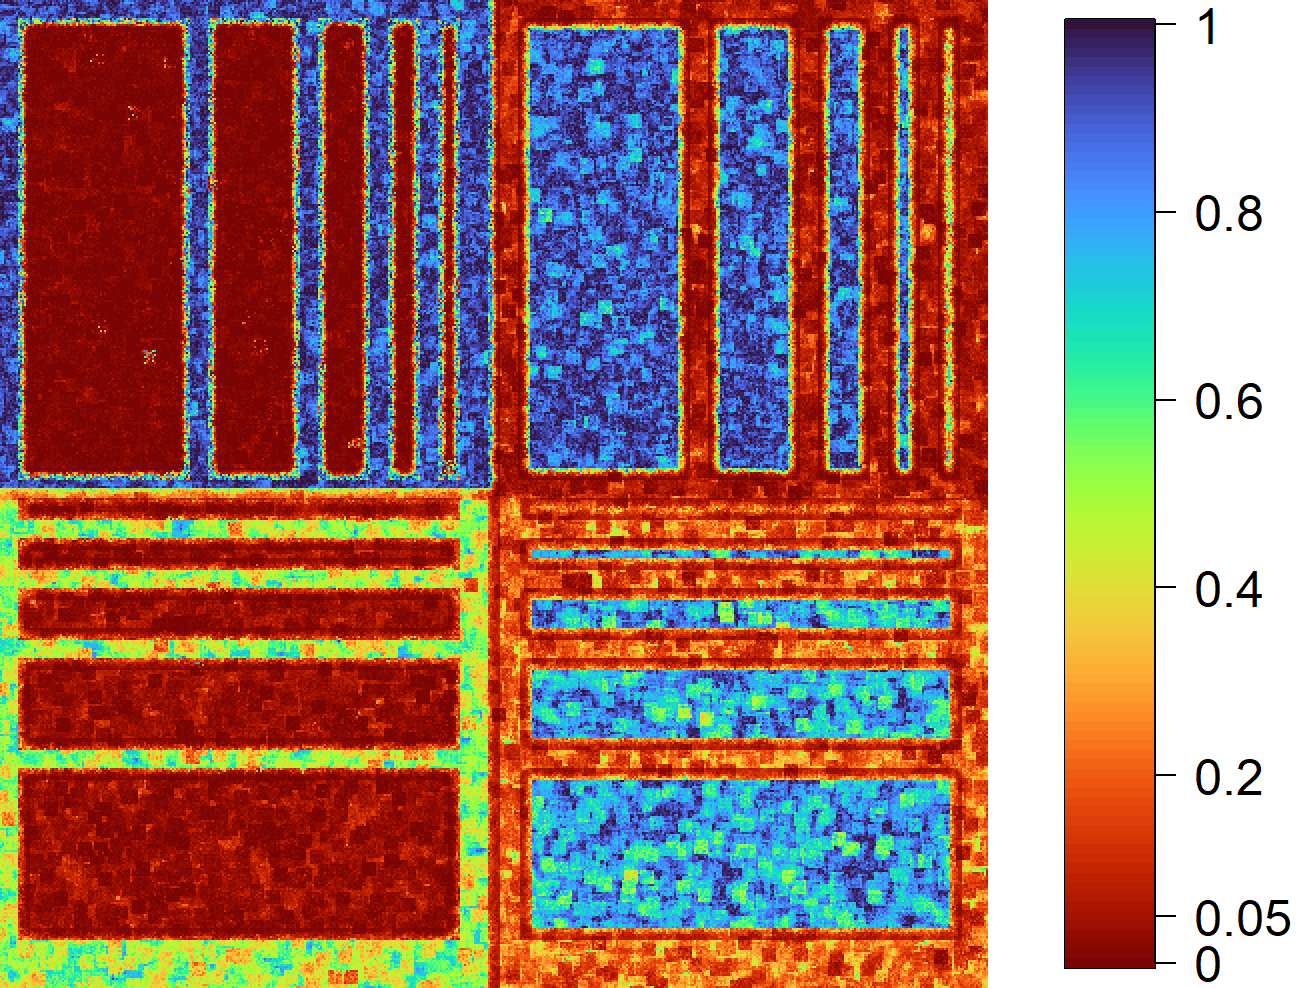
\includegraphics[width=\linewidth]{./Figures/p-values__sim_L18_lambda085_7x7.png}
\caption{$p$-value map ($7\times7$)}
\label{fig:simc1}
\end{subfigure}\hfill
\begin{subfigure}[t]{0.19\textwidth}
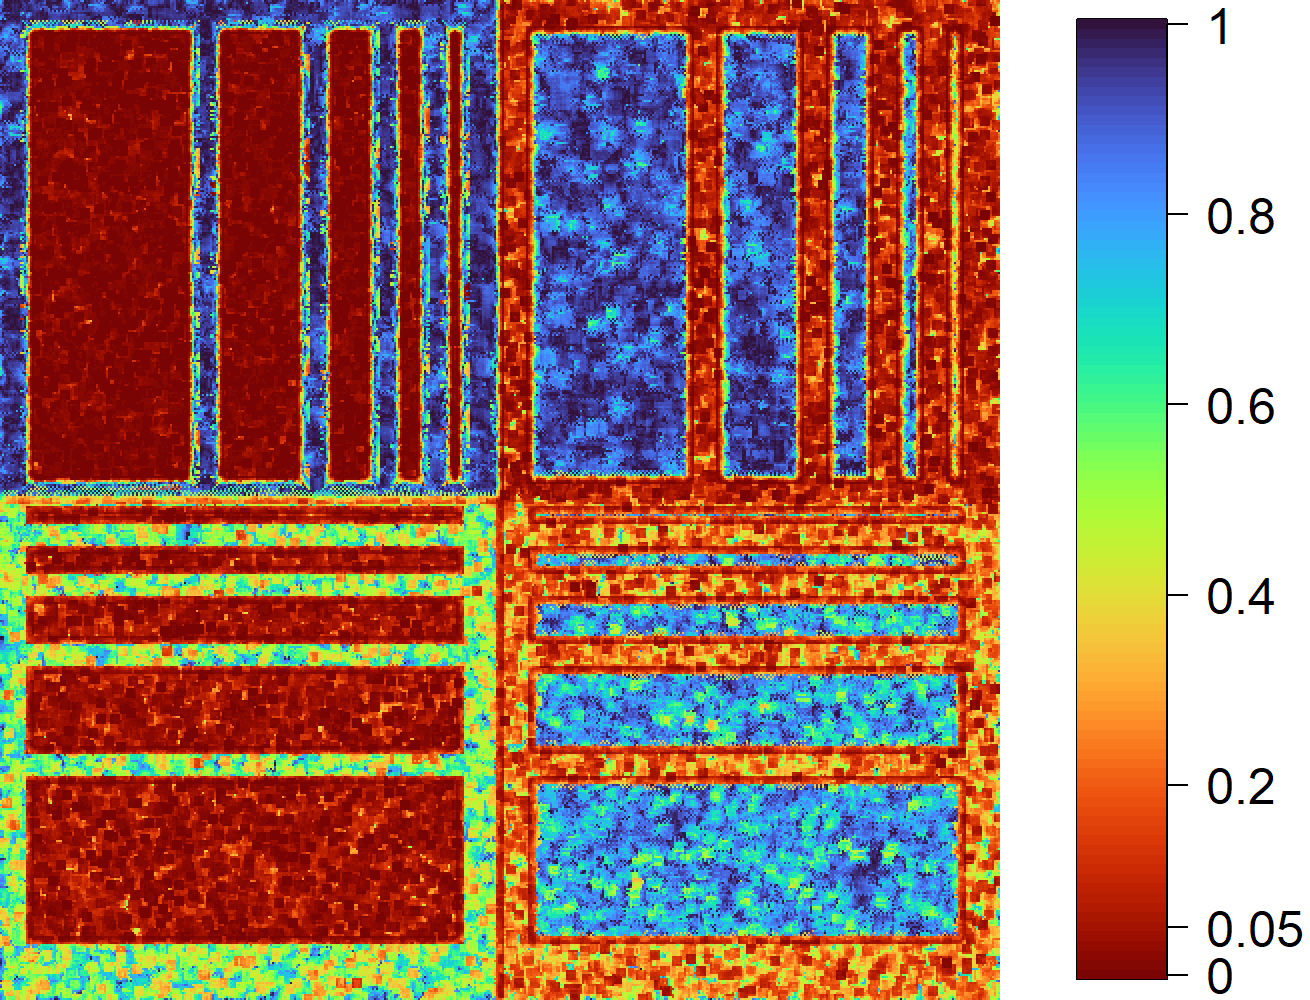
\includegraphics[width=\linewidth]{./Figures/p-values_sim_L18_6_w200_eta1.0_lambda085_5x11.png}
\caption{$p$-value map ($\eta=1$)}
\label{fig:simc2}
\end{subfigure}\hfill
\begin{subfigure}[t]{0.19\textwidth}
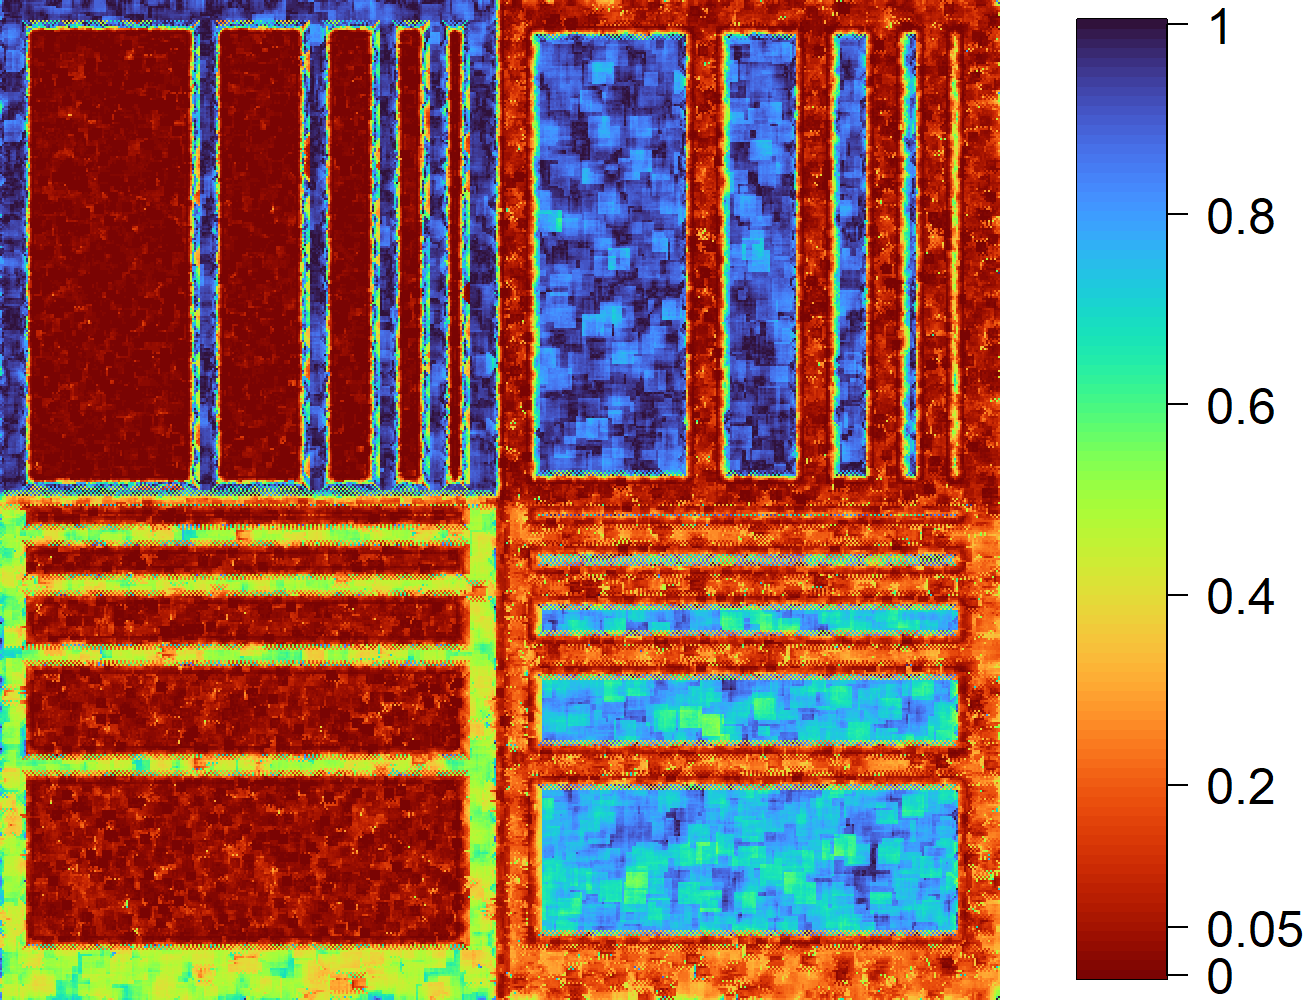
\includegraphics[width=\linewidth]{./Figures/p-values_sim_L18_6_w200_eta2_lambda085_5x11.png}
\caption{$p$-value map ($\eta=2$)}
\label{fig:simc3}
\end{subfigure}\hfill
\begin{subfigure}[t]{0.19\textwidth}
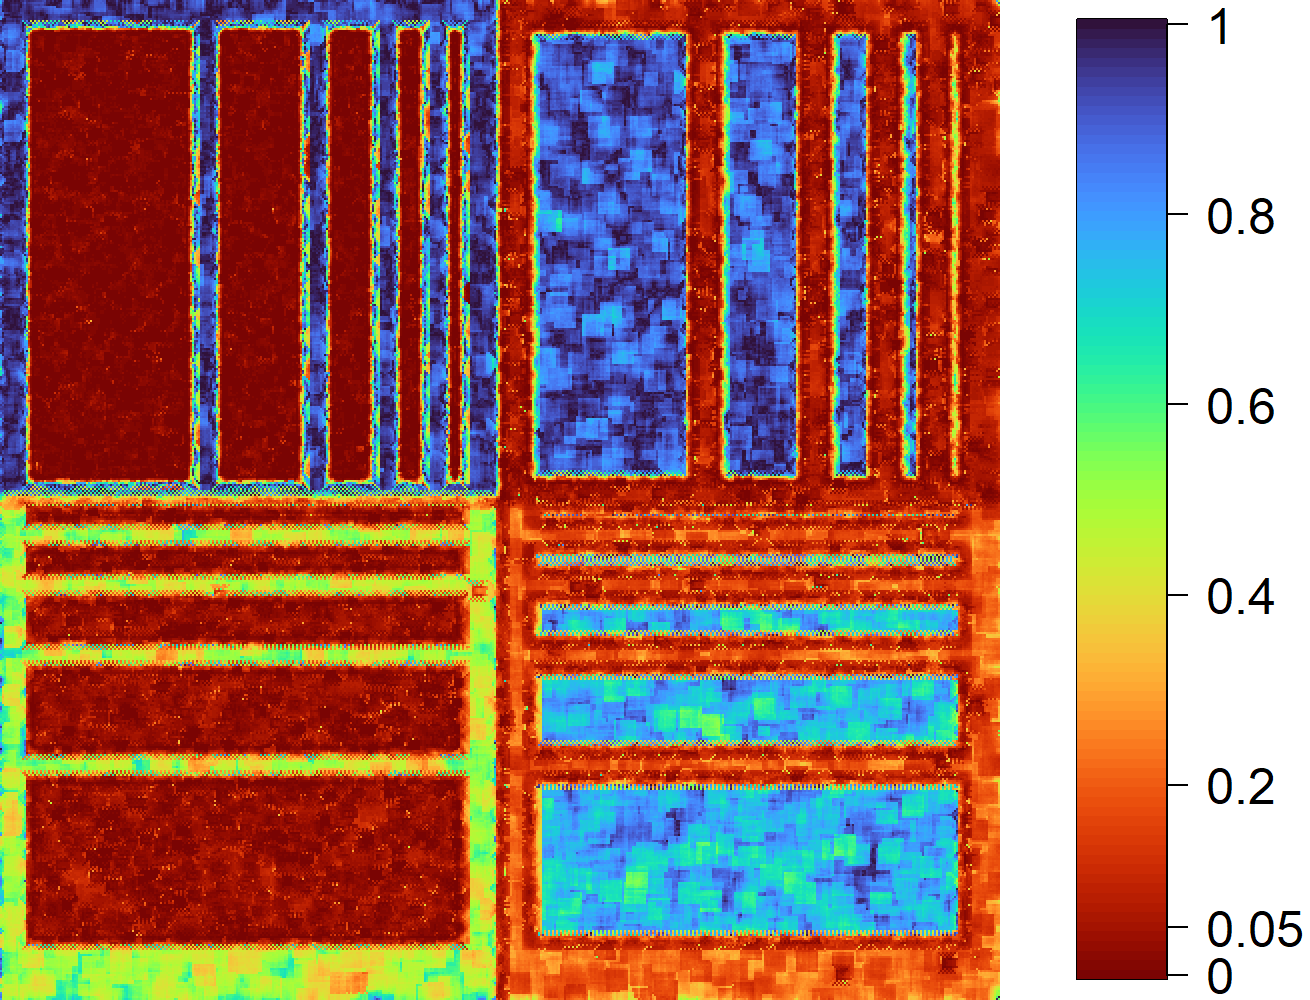
\includegraphics[width=\linewidth]{./Figures/p-values_sim_L18_6_w200_eta3.0_lambda085_5x11.png}
\caption{$p$-value map ($\eta=3$)}
\label{fig:simc4}
\end{subfigure}\hfill
\begin{subfigure}[t]{0.19\textwidth}
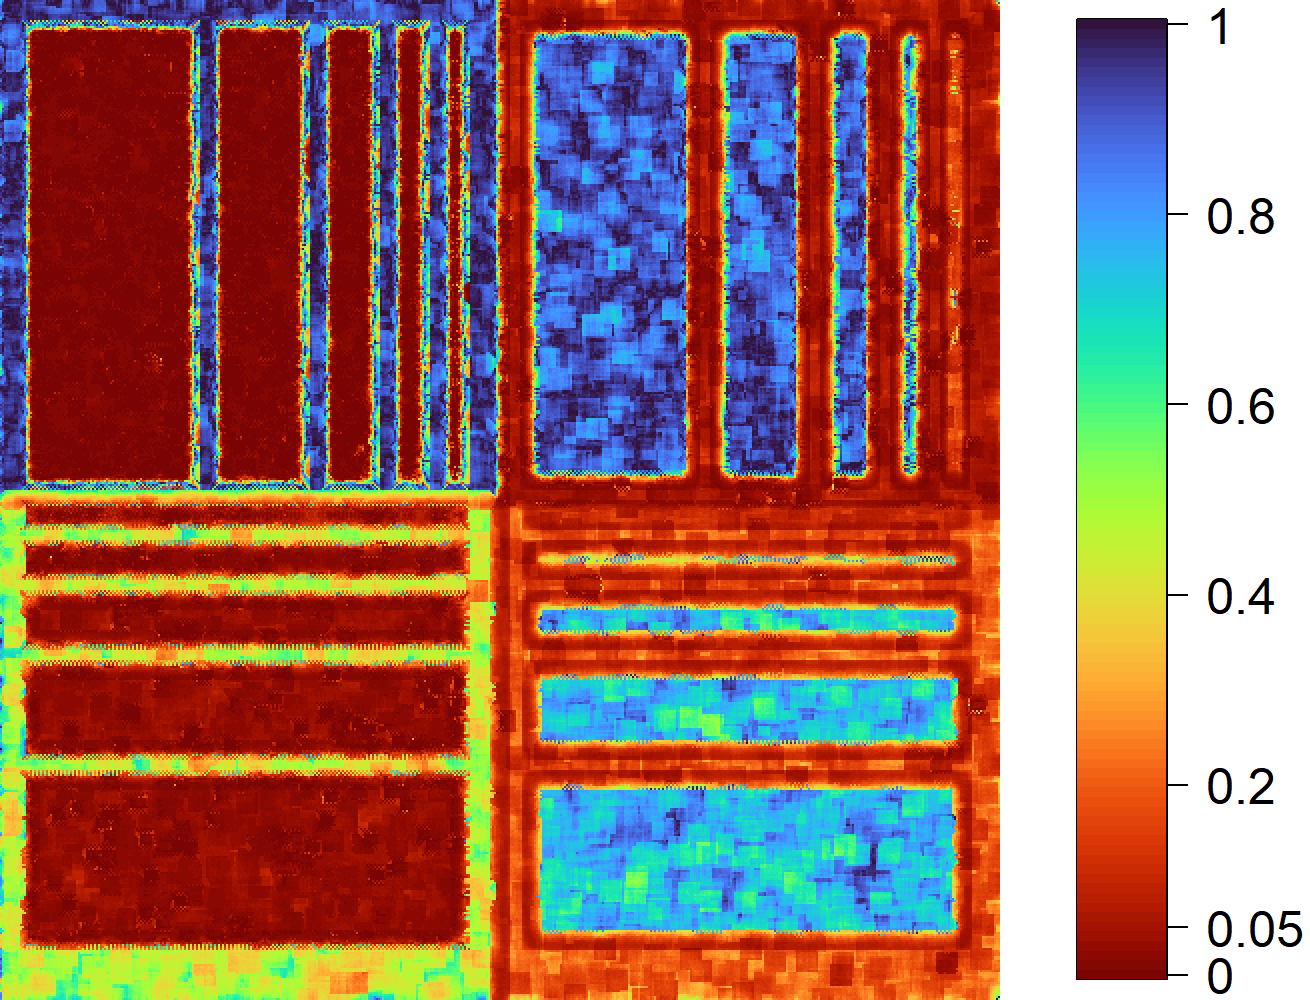
\includegraphics[width=\linewidth]{./Figures/p-values_Sim_L18_eta4.png}
\caption{$p$-value map ($\eta=4$)}
\label{fig:simc5}
\end{subfigure}

\vspace{4pt}

\begin{subfigure}[t]{0.19\textwidth}
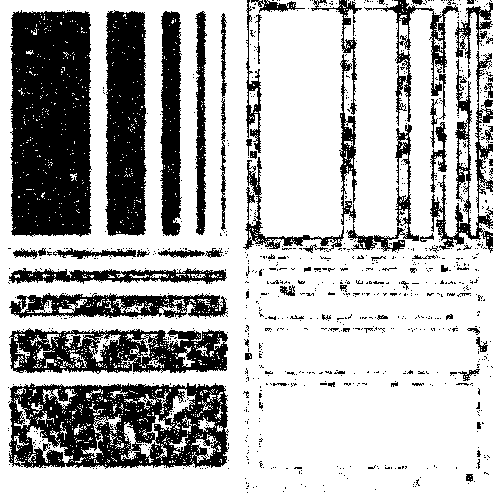
\includegraphics[width=\linewidth]{./Figures/H_005_sim_L18_lambda085_7x7.png}
\caption{Binary map ($7\times7$)}
\label{fig:simbc1}
\end{subfigure}\hfill
\begin{subfigure}[t]{0.19\textwidth}
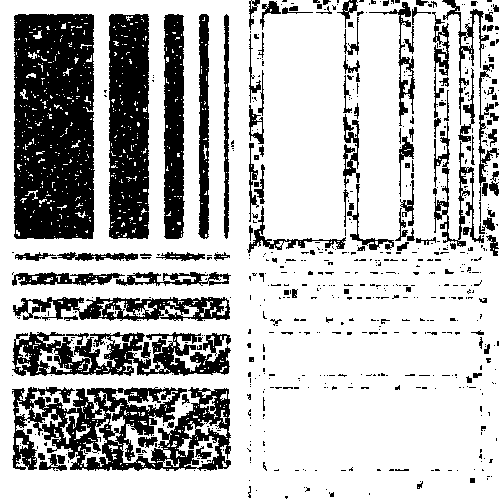
\includegraphics[width=\linewidth]{./Figures/H_005_sim_L18_6_w200_eta1.0_lambda085_5x11.png}
\caption{Binary map ($\eta=1$)}
\label{fig:simbc2}
\end{subfigure}\hfill
\begin{subfigure}[t]{0.19\textwidth}
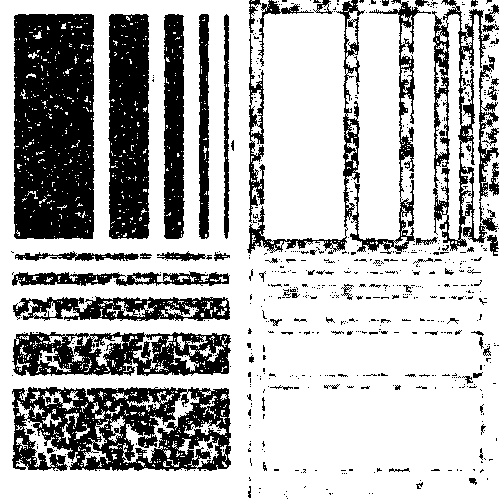
\includegraphics[width=\linewidth]{./Figures/H_005_sim_L18_6_w200_eta2_lambda085_5x11.png}
\caption{Binary map ($\eta=2$)}
\label{fig:simbc3}
\end{subfigure}\hfill
\begin{subfigure}[t]{0.19\textwidth}
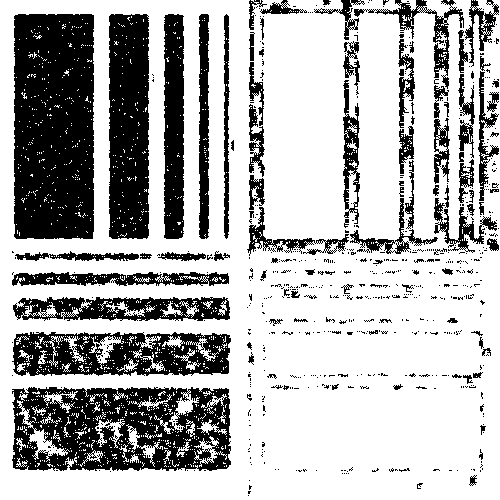
\includegraphics[width=\linewidth]{./Figures/H_005_sim_L18_6_w200_eta3.0_lambda085_5x11.png}
\caption{Binary map ($\eta=3$)}
\label{fig:simbc4}
\end{subfigure}\hfill
\begin{subfigure}[t]{0.19\textwidth}
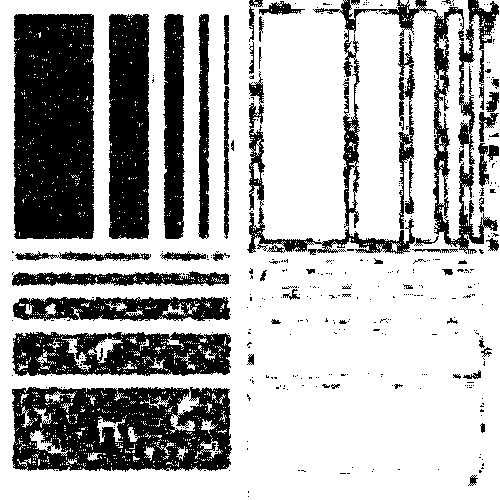
\includegraphics[width=\linewidth]{./Figures/H_005_Sim_L18_eta4.png}
\caption{Binary map ($\eta=4$)}
\label{fig:simbc5}
\end{subfigure}

\caption{Simulated-scene results with the test $S_{\widetilde{T}_{\lambda}}$. (a) $p$-value map with a fixed $7\times7$ window. (b–e) $p$-value maps with adaptive windows ($W_{\min}=5$, $W_{\max}=11$) for $\eta=1$--$4$. (f–j) Binary decision maps at $0.05$ significance level.}
\label{fig:grid10}
\end{figure*}

\subsection{SAR dataset}\label{sar-dataset}

We evaluated the proposed test statistic on four SAR scenes from
different radar missions, covering San Francisco (USA), the outskirts of
Munich (Germany), Dublin Port (Ireland), and the area around Foggia
(Italy). The first three SAR images were acquired in HH polarization
from two different sensors (an airborne and a spaceborne one) and the
fourth in VV polarization (see Figures~\ref{fig:sar1}, \ref{fig:sar2},
\ref{fig:sar3} and \ref{fig:sar4}). The corresponding optical images
(Figures~\ref{fig:opt1}, \ref{fig:opt2}, \ref{fig:opt3} and
\ref{fig:opt4}) show the corresponding land cover context.

\setlength{\dblfloatsep}{4pt}      
\setlength{\dbltextfloatsep}{4pt}  
\setlength{\textfloatsep}{4pt}
\captionsetup{font=footnotesize}
\captionsetup[sub]{aboveskip=1pt,belowskip=1pt}

\begin{figure*}[!t]
\centering
\captionsetup{font=footnotesize}
\captionsetup[sub]{aboveskip=2pt,belowskip=2pt}
\begin{subfigure}[t]{0.19\textwidth}
  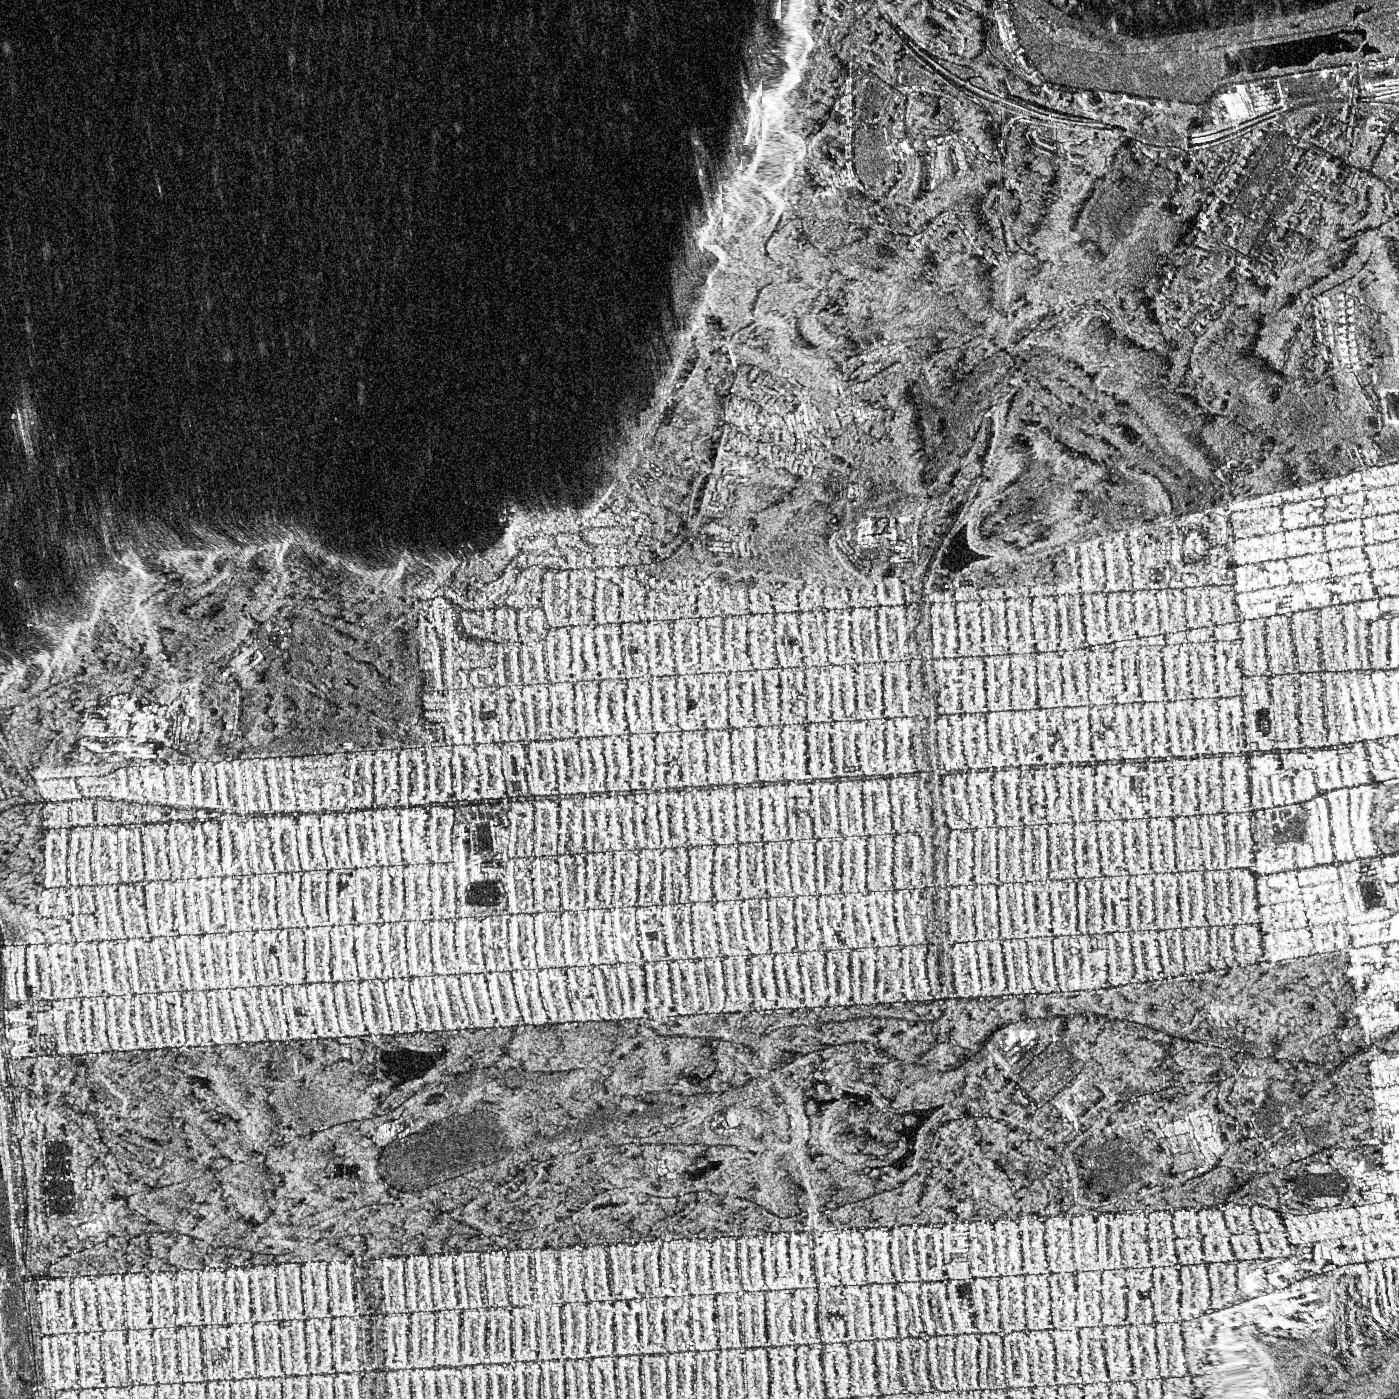
\includegraphics[width=\linewidth]{./Figures/sanFrancisco1400.png}
  \caption{SAR image (San Francisco)}
  \label{fig:sar1}
\end{subfigure}
\hspace{0.01\textwidth}%\hfill
\begin{subfigure}[t]{0.181\textwidth}
  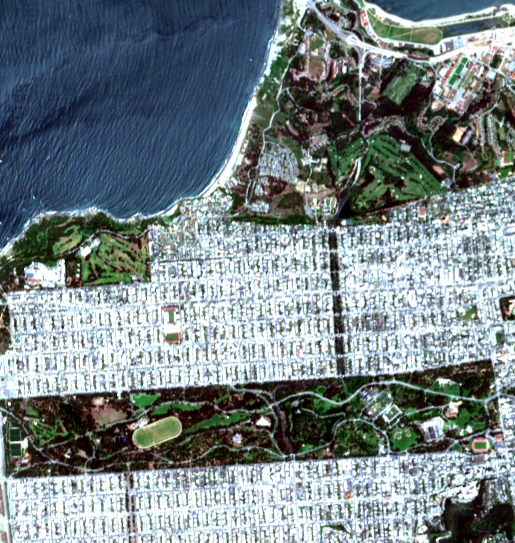
\includegraphics[width=\linewidth]{./Figures/san-francisco-optical.png}
  \caption{Optical image (San Francisco)}
  \label{fig:opt1}
\end{subfigure}
\hspace{0.01\textwidth}%\hfill
\begin{subfigure}[t]{0.19\textwidth}
  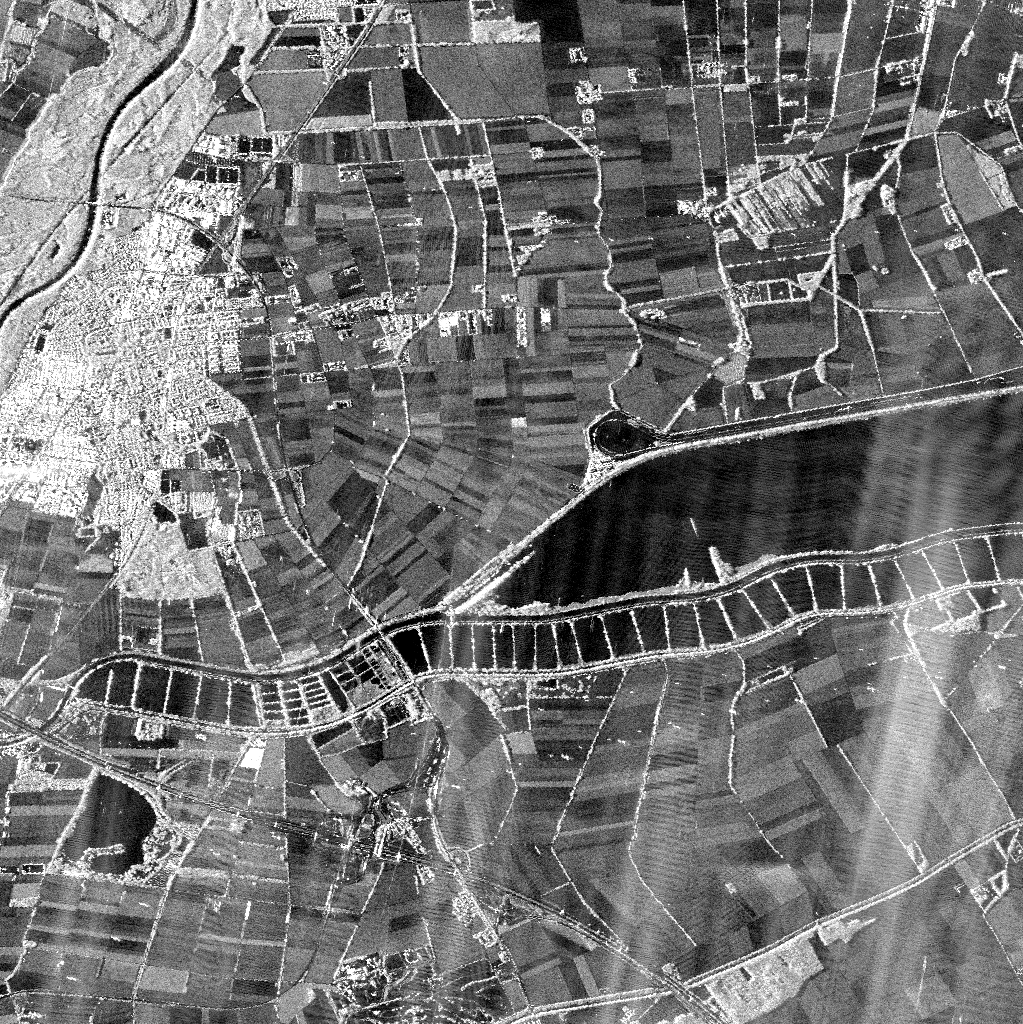
\includegraphics[width=\linewidth]{./Figures/munich_1024.png}
  \caption{SAR image (Munich)}
  \label{fig:sar2}
\end{subfigure}
\hspace{0.01\textwidth}%\hfill
\begin{subfigure}[t]{0.18\textwidth}
  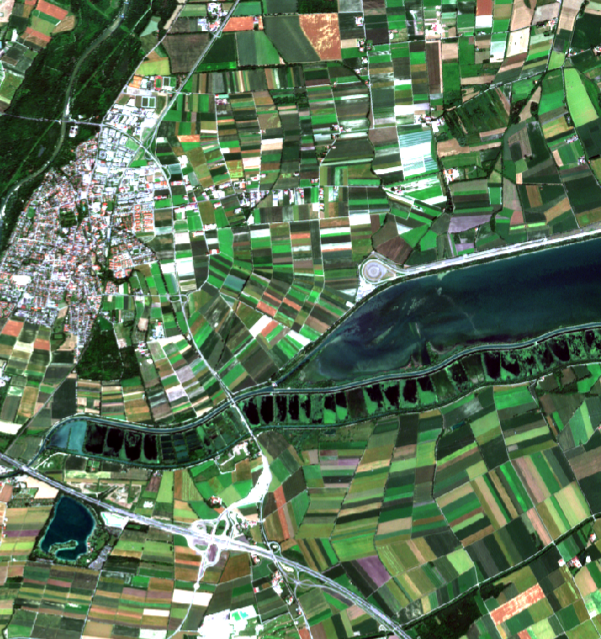
\includegraphics[width=\linewidth]{./Figures/munich_optical.png}
  \caption{Optical image (Munich)}
  \label{fig:opt2}
\end{subfigure}

\medskip 
\vspace{-4pt}

\begin{subfigure}[t]{0.19\textwidth}
  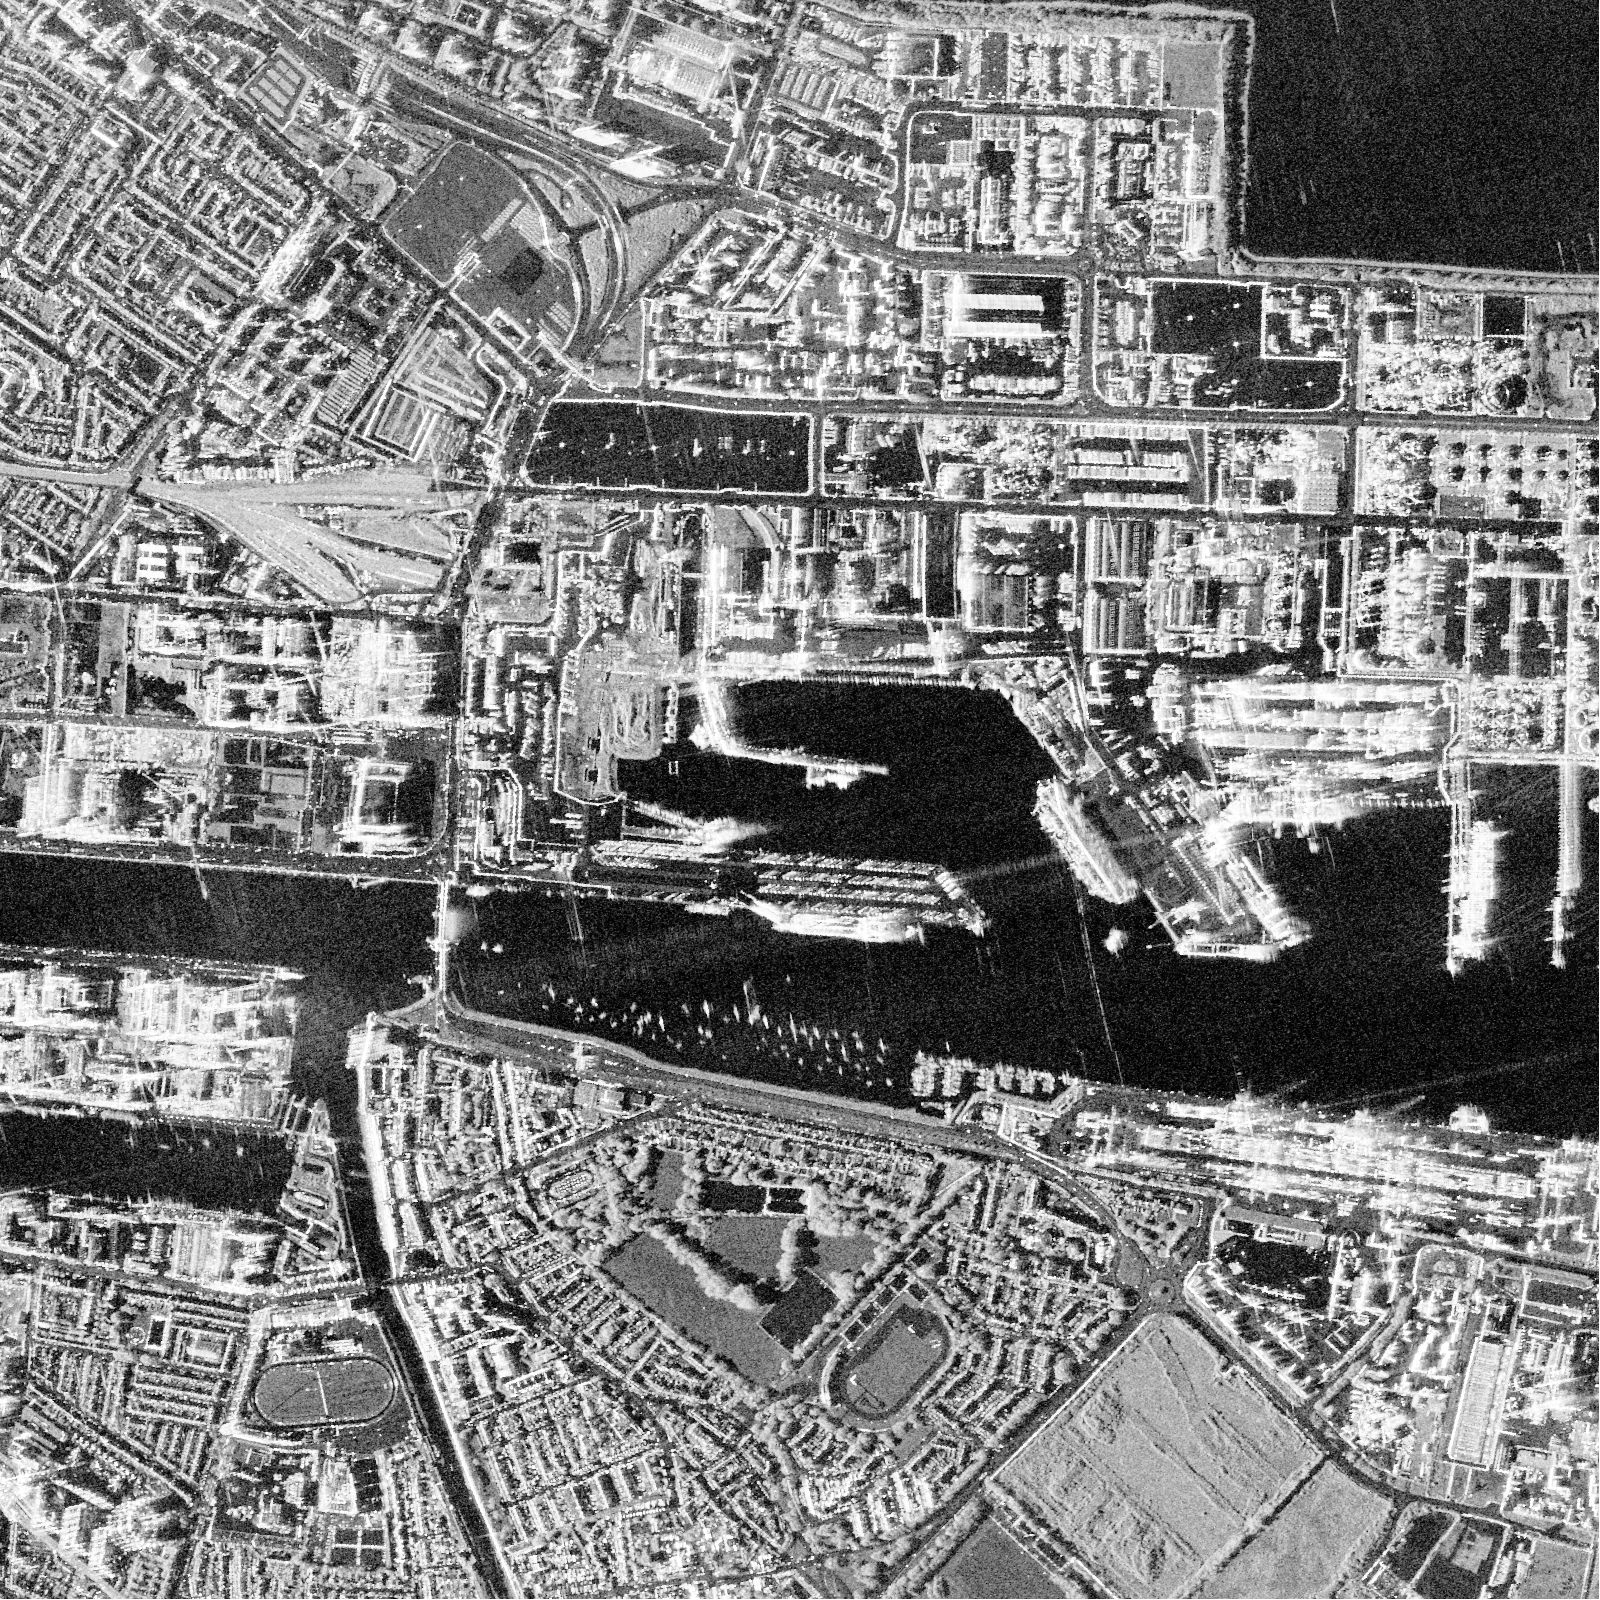
\includegraphics[width=\linewidth]{./Figures/dubli_1600.png}
  \caption{SAR image (Dublin Port)}
  \label{fig:sar3}
\end{subfigure}
\hspace{0.001\textwidth}%\hfill
\begin{subfigure}[t]{0.196\textwidth}
  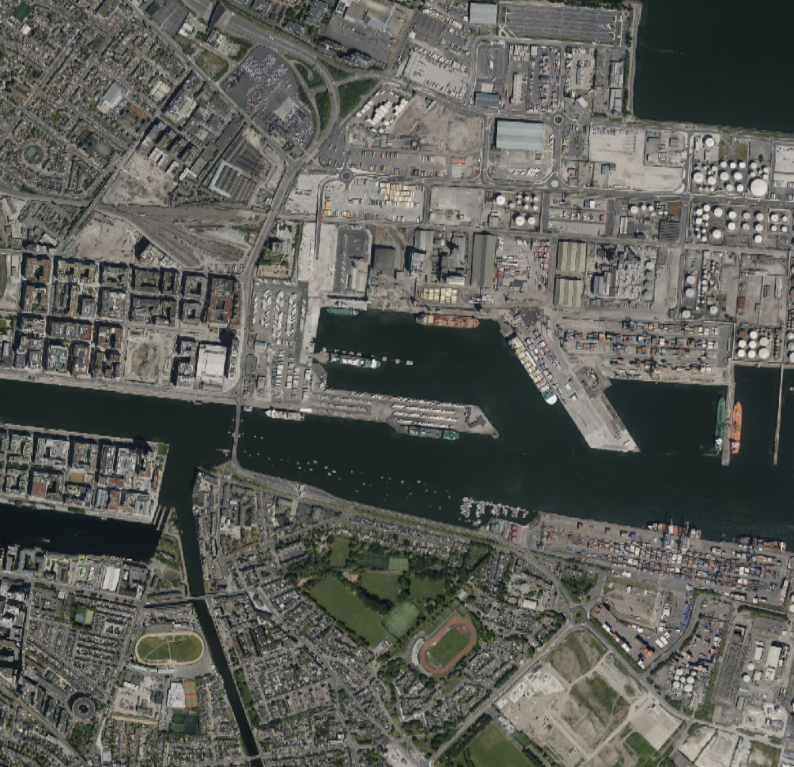
\includegraphics[width=\linewidth]{./Figures/dublin_optical1.png}
  \caption{Optical image (Dublin Port)}
  \label{fig:opt3}
\end{subfigure}
\hspace{0.001\textwidth}%\hfill
\begin{subfigure}[t]{0.19\textwidth}
  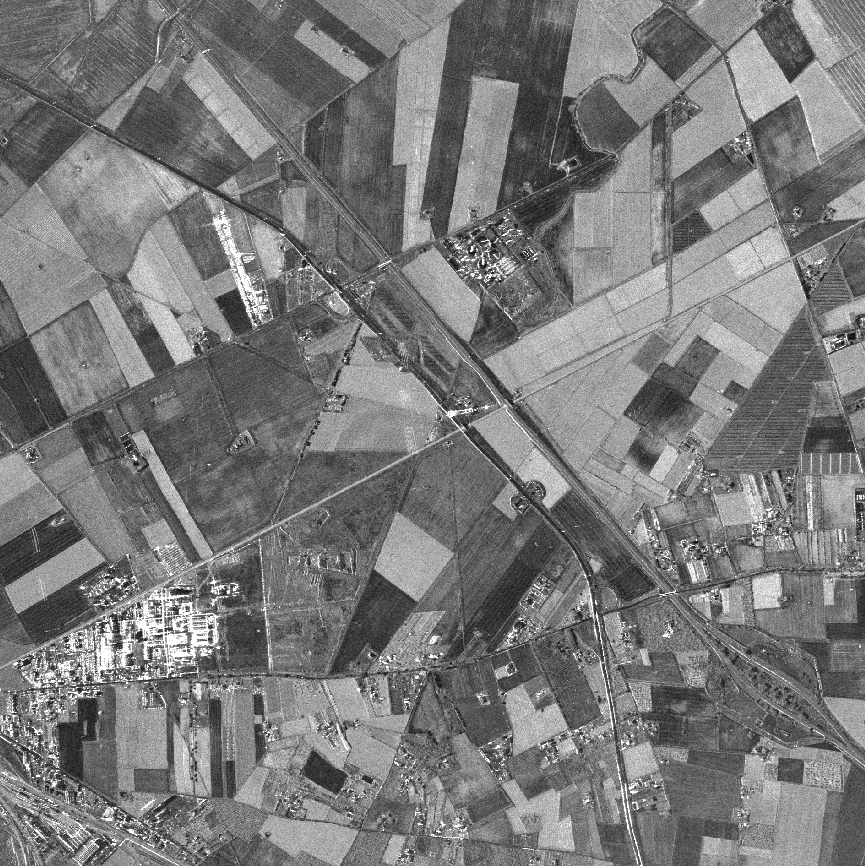
\includegraphics[width=\linewidth]{./Figures/Foggia_new.png}
  \caption{SAR image (Foggia)}
  \label{fig:sar4}
\end{subfigure}
\hspace{0.001\textwidth}
\begin{subfigure}[t]{0.187\textwidth}
  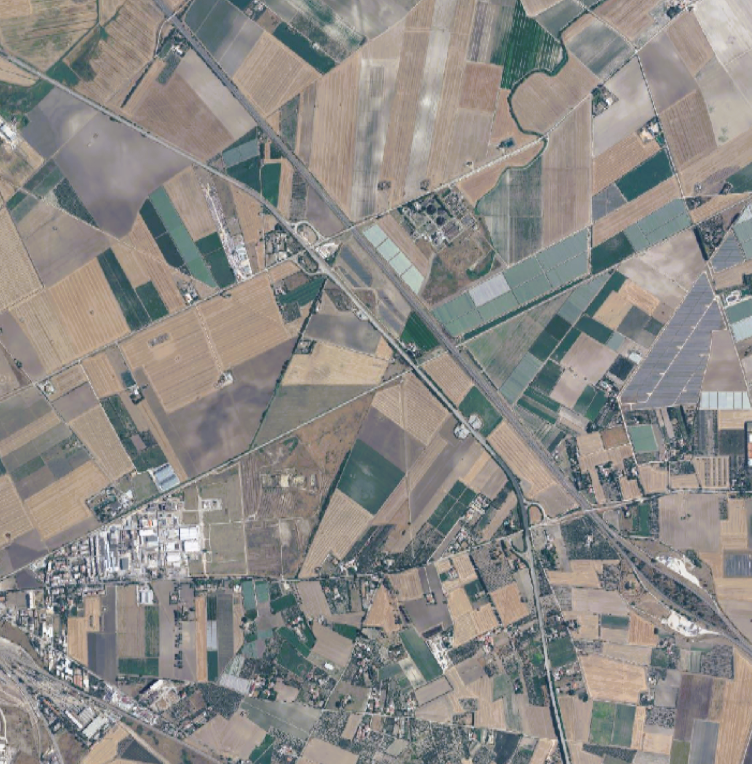
\includegraphics[width=\linewidth]{./Figures/foggia-italy-optical.png}
  \caption{Optical image (Foggia)}
  \label{fig:opt4}
\end{subfigure}
%\hspace{0.001\textwidth}
\caption{SAR and optical images.}

\label{fig:images}
\end{figure*}

The SAR scenes come from different missions: PAZ, TanDEM-X, UAVSAR, and
Iceye. All images are single-polarization (HH or VV), and their
acquisition parameters vary in resolution, scene size, and number of
looks. Table~\ref{tab:table_param} reports the acquisition parameters.

\renewcommand{\arraystretch}{2.5}

\begin{table}[hbt]
\centering
\DIFdelbeginFL %DIFDELCMD < \centering
%DIFDELCMD < %%%
\DIFdelendFL \caption{\label{tab:table_param}Parameters of selected SAR images.}
\centering
\DIFdelbeginFL %DIFDELCMD < \resizebox{\ifdim\width>\linewidth\linewidth\else\width\fi}{!}{
%DIFDELCMD < \fontsize{24}{26}\selectfont
%DIFDELCMD < \begin{tabu} to \linewidth {>{\centering\arraybackslash}p{4.0cm}>{\centering\arraybackslash}p{4.3cm}>{\centering\arraybackslash}p{1.5cm}>{\centering\arraybackslash}p{4cm}>{\centering\arraybackslash}p{1.5cm}>{\centering\arraybackslash}p{4.0cm}>{\centering\arraybackslash}p{4.0cm}}
%DIFDELCMD < \toprule
%DIFDELCMD < \multicolumn{1}{c}{\textbf{Scene}} & \multicolumn{1}{c}{\textbf{Mission}} & \multicolumn{1}{c}{\textbf{Band}} & \multicolumn{1}{c}{\textbf{Size (pixels)}} & \multicolumn{1}{c}{$\bm{L}$} & \multicolumn{1}{c}{\textbf{Resolution [m]}} & \multicolumn{1}{c}{\textbf{Acquisition Date}}\\
%DIFDELCMD < \midrule
%DIFDELCMD < San Francisco & PAZ & X & $1400\times1400$ & $4$ & $3.6\times3.6$ & 03-01-2020\\
%DIFDELCMD < Munich & UAVSAR & L & $1024\times1024$ & $12$ & $4.9\times7.2$ & 16-04-2015\\
%DIFDELCMD < Dublin & TanDEM-X & X & $1600\times1600$ & $16$ & $1.35\times1.35$ & 03-09-2017\\
%DIFDELCMD < Foggia & Iceye & X & $1900\times1900$ & $24$ & $2.08\times2.08$ & 28-03-2024\\
%DIFDELCMD < \bottomrule
%DIFDELCMD < \end{tabu}}
%DIFDELCMD < %%%
\DIFdelendFL \DIFaddbeginFL \resizebox{\ifdim\width>\linewidth\linewidth\else\width\fi}{!}{
\fontsize{24}{26}\selectfont
\begin{tabular}[t]{>{\centering\arraybackslash}p{4.0cm}>{\centering\arraybackslash}p{4.3cm}>{\centering\arraybackslash}p{1.5cm}>{\centering\arraybackslash}p{4cm}>{\centering\arraybackslash}p{1.5cm}>{\centering\arraybackslash}p{4.0cm}>{\centering\arraybackslash}p{4.0cm}}
\toprule
\multicolumn{1}{c}{\textbf{Scene}} & \multicolumn{1}{c}{\textbf{Mission}} & \multicolumn{1}{c}{\textbf{Band}} & \multicolumn{1}{c}{\textbf{Size (pixels)}} & \multicolumn{1}{c}{$\bm{L}$} & \multicolumn{1}{c}{\textbf{Resolution [m]}} & \multicolumn{1}{c}{\textbf{Acquisition Date}}\\
\midrule
San Francisco & PAZ & X & $1400\times1400$ & $4$ & $3.6\times3.6$ & 03-01-2020\\
Munich & UAVSAR & L & $1024\times1024$ & $12$ & $4.9\times7.2$ & 16-04-2015\\
Dublin & TanDEM-X & X & $1600\times1600$ & $16$ & $1.35\times1.35$ & 03-09-2017\\
Foggia & Iceye & X & $1900\times1900$ & $24$ & $2.08\times2.08$ & 28-03-2024\\
\bottomrule
\end{tabular}}
\DIFaddendFL \end{table}

For each SAR image, the number of looks \(L\) was obtained from the
product of azimuth and range looks provided in the metadata of SNAP
(Sentinel Application Platform) toolbox. We validated this nominal value
with the equivalent number of looks (ENL) from manually selected
homogeneous areas using the classical formula
\(\text{ENL} = 1/\widehat{\text{CV}}^2\), based on the sample
coefficient of variation. The results were consistent with the metadata.
We also verified that moderate deviations in \(L\) did not significantly
impact the outcome of the test, confirming the robustness of the
proposed method.

\subsection{Qualitative analysis}\label{qualitative-analysis}

The proposed Tsallis-based test statistic,
\(S_{\widetilde{T}_{\lambda}}\), was applied to four SAR intensity
images. For each scene, results were obtained using a fixed \(7\times7\)
sliding window and the adaptive windowing scheme with side lengths
ranging from \(5\times5\) (\(W_{\min}=5\)) to \(11\times11\)
(\(W_{\max}=11\)), for smoothing parameters \(\eta=1\), \(2\), \(3\),
and \(4\). In all cases, \(B=100\) bootstrap replications were performed
per window.

Figures~\ref{fig:sanfrancisco}--\ref{fig:foggia} present the outcomes,
organized in two rows: the first row shows the \(p\)-value maps, while
the second row displays the corresponding binary decision maps at the
\(0.05\) significance level, where black pixels denote heterogeneous
areas and white pixels homogeneous regions.

\setlength{\dblfloatsep}{4pt}      
\setlength{\dbltextfloatsep}{4pt}  
\setlength{\textfloatsep}{4pt}
\captionsetup{font=footnotesize}
\captionsetup[sub]{aboveskip=1pt,belowskip=1pt}

\begin{figure*}[!t]
\centering

\captionsetup{font=footnotesize}
\captionsetup[sub]{aboveskip=2pt,belowskip=2pt}

\begin{subfigure}[t]{0.19\textwidth}
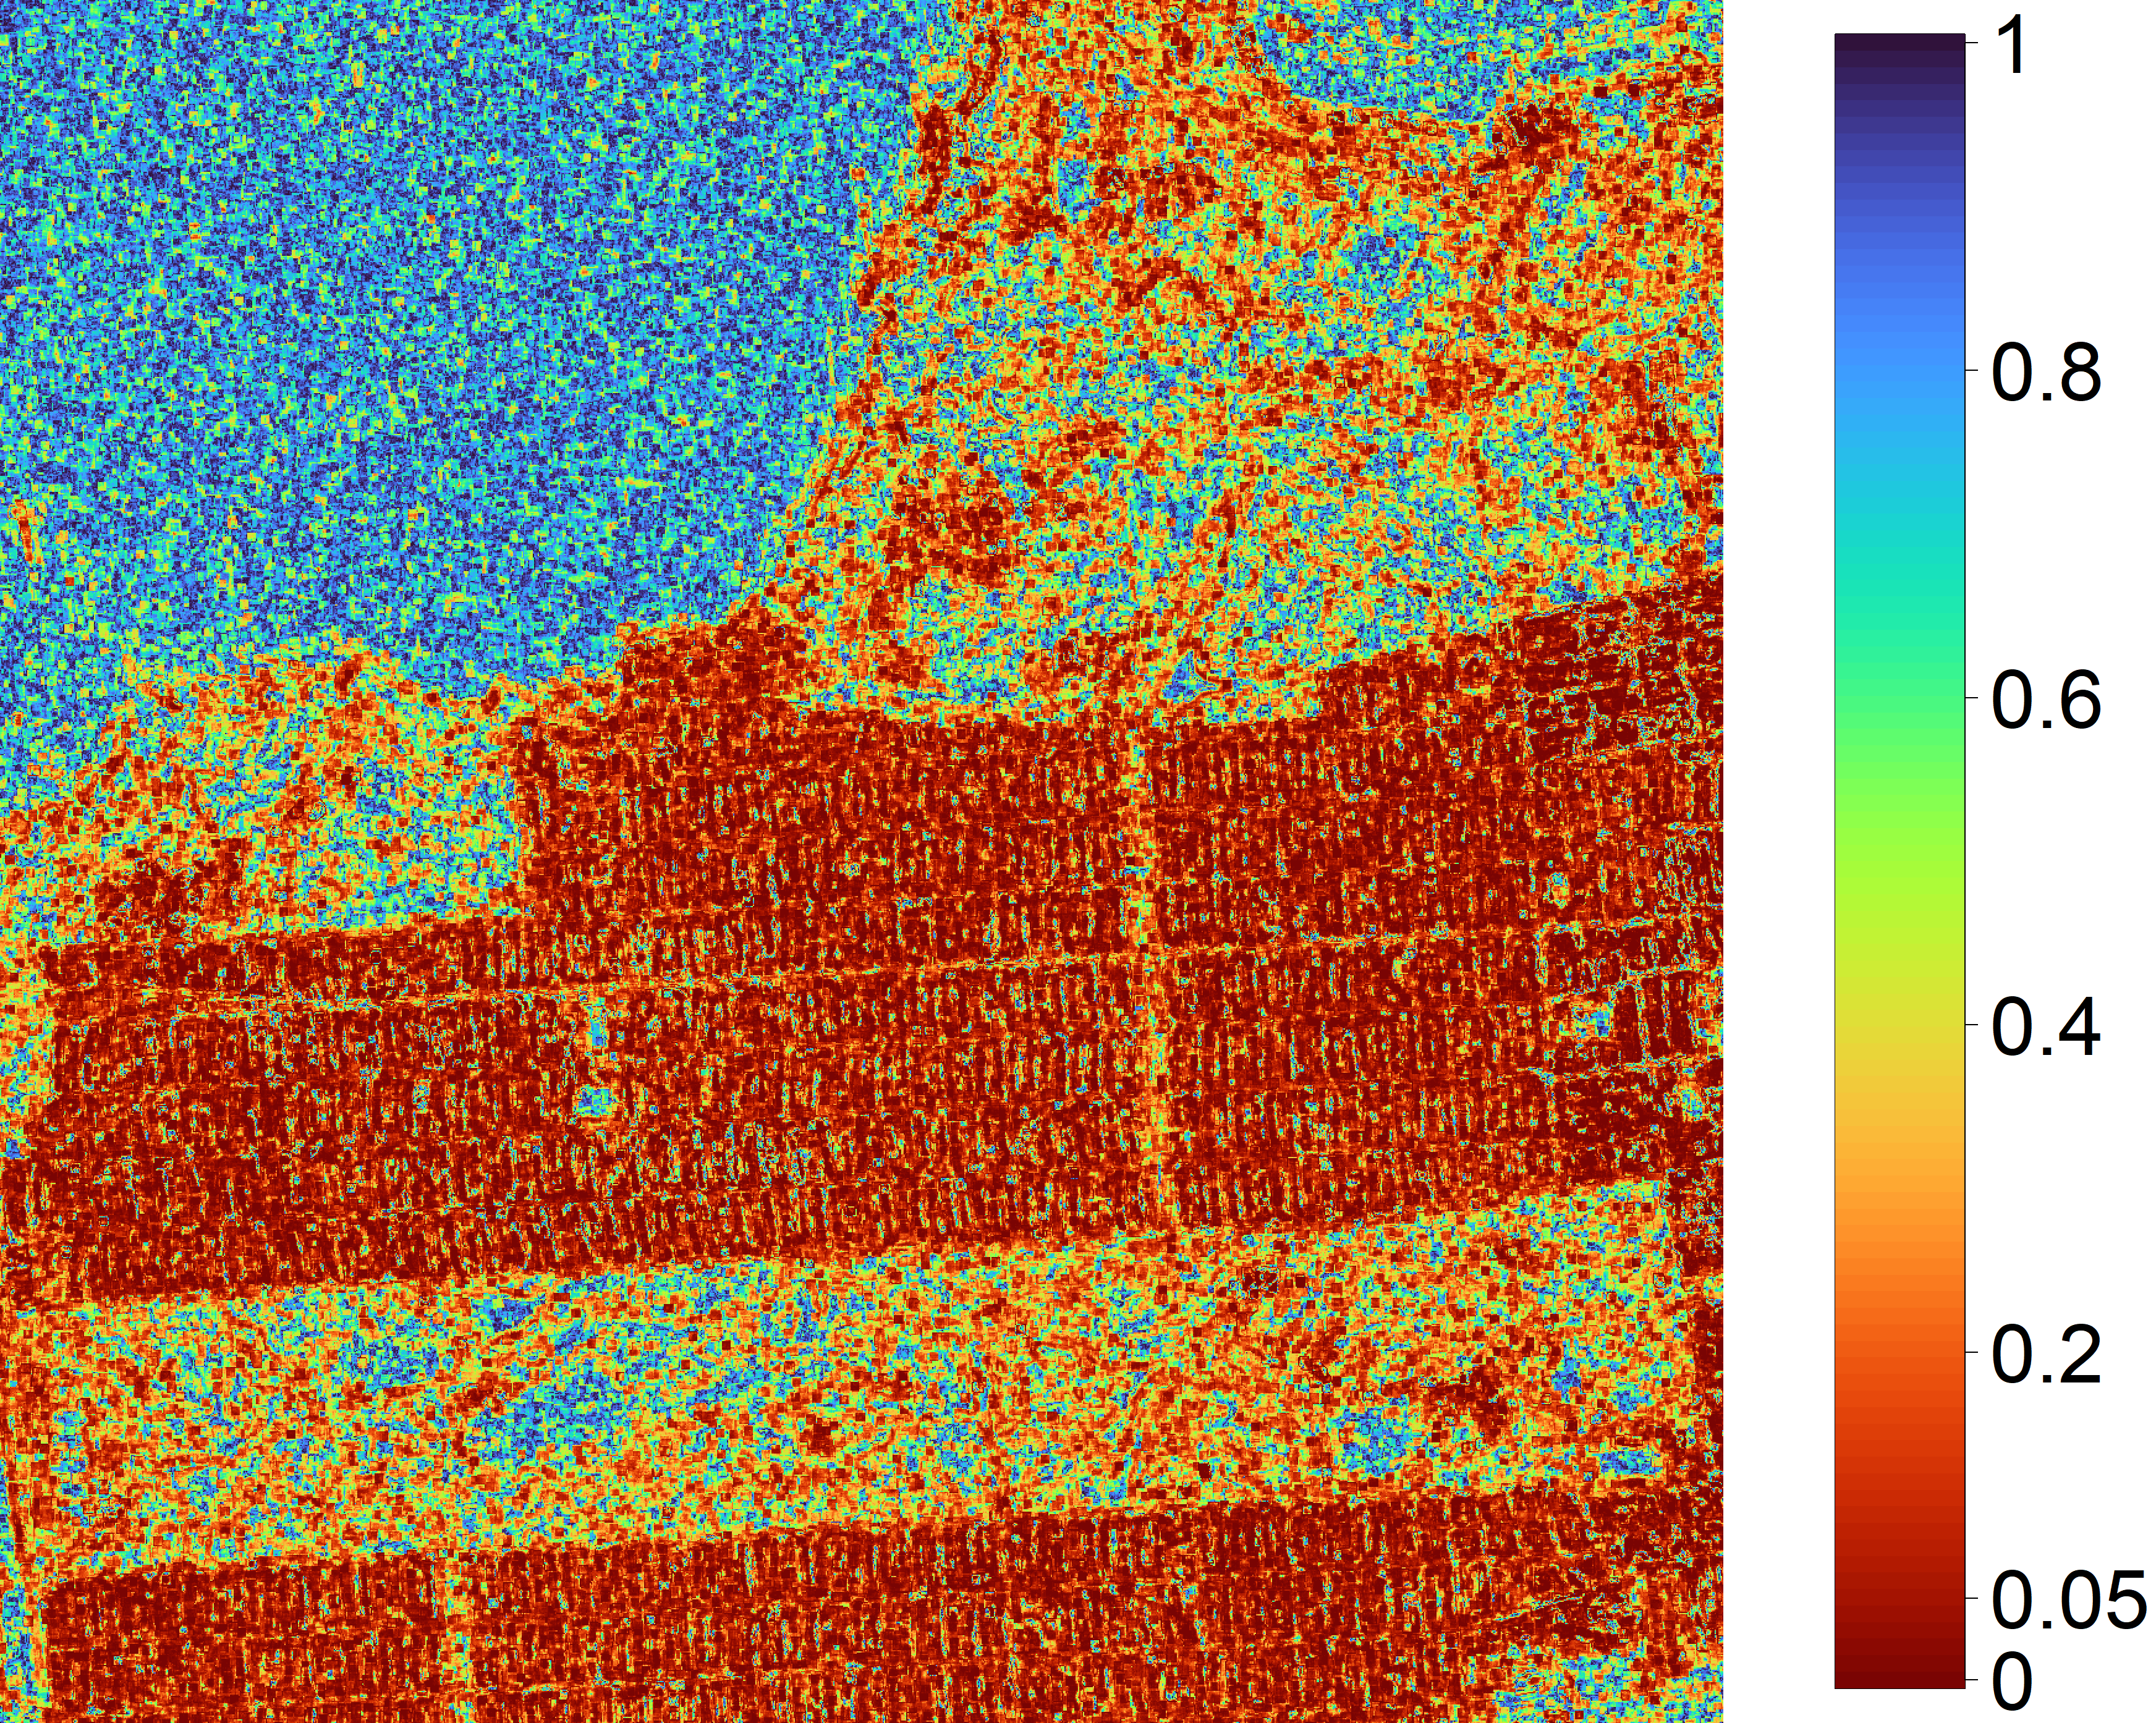
\includegraphics[width=\linewidth]{./Figures/p-values_San-fran1400-fijo-7x7.png}
\caption{$p$-value map ($7\times7$)}
\label{fig:SFc1}
\end{subfigure}\hfill
\begin{subfigure}[t]{0.19\textwidth}
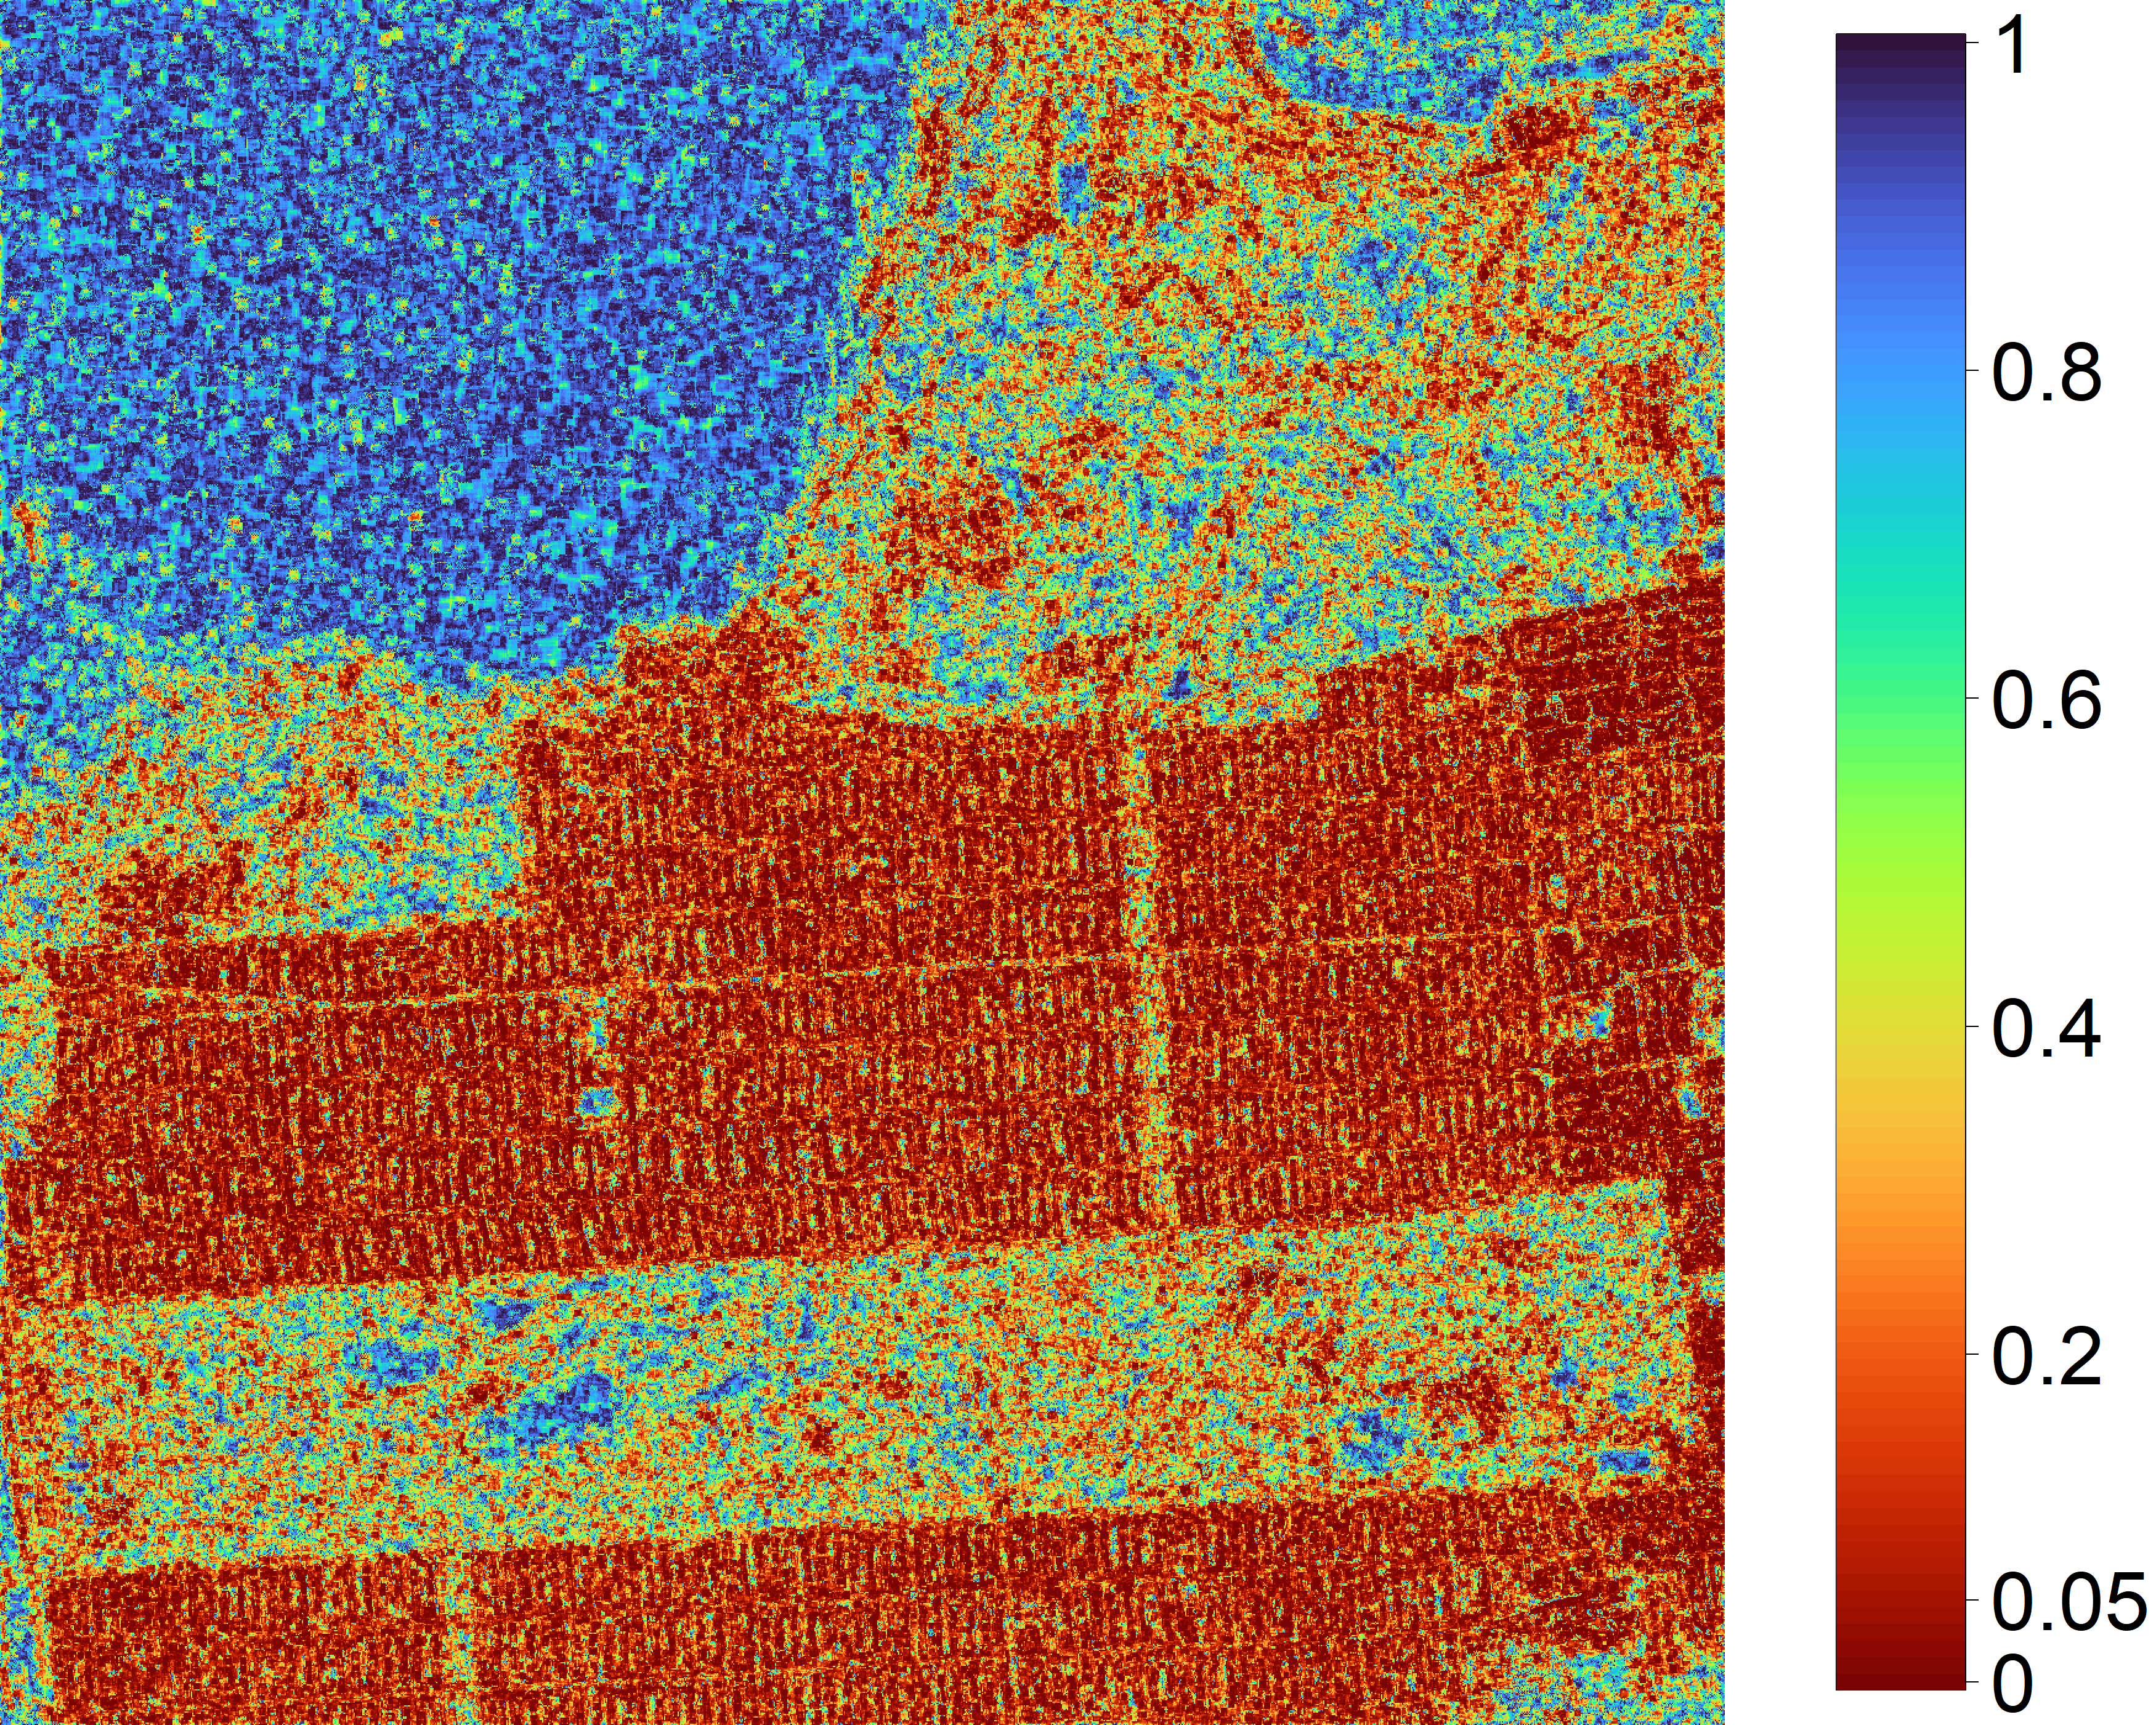
\includegraphics[width=\linewidth]{./Figures/p-values_San-fran1400_eta1.0_B100_lambda_085-5x11_L4_1.png}
\caption{$p$-value map ($\eta=1$)}
\label{fig:SFc2}
\end{subfigure}\hfill
\begin{subfigure}[t]{0.19\textwidth}
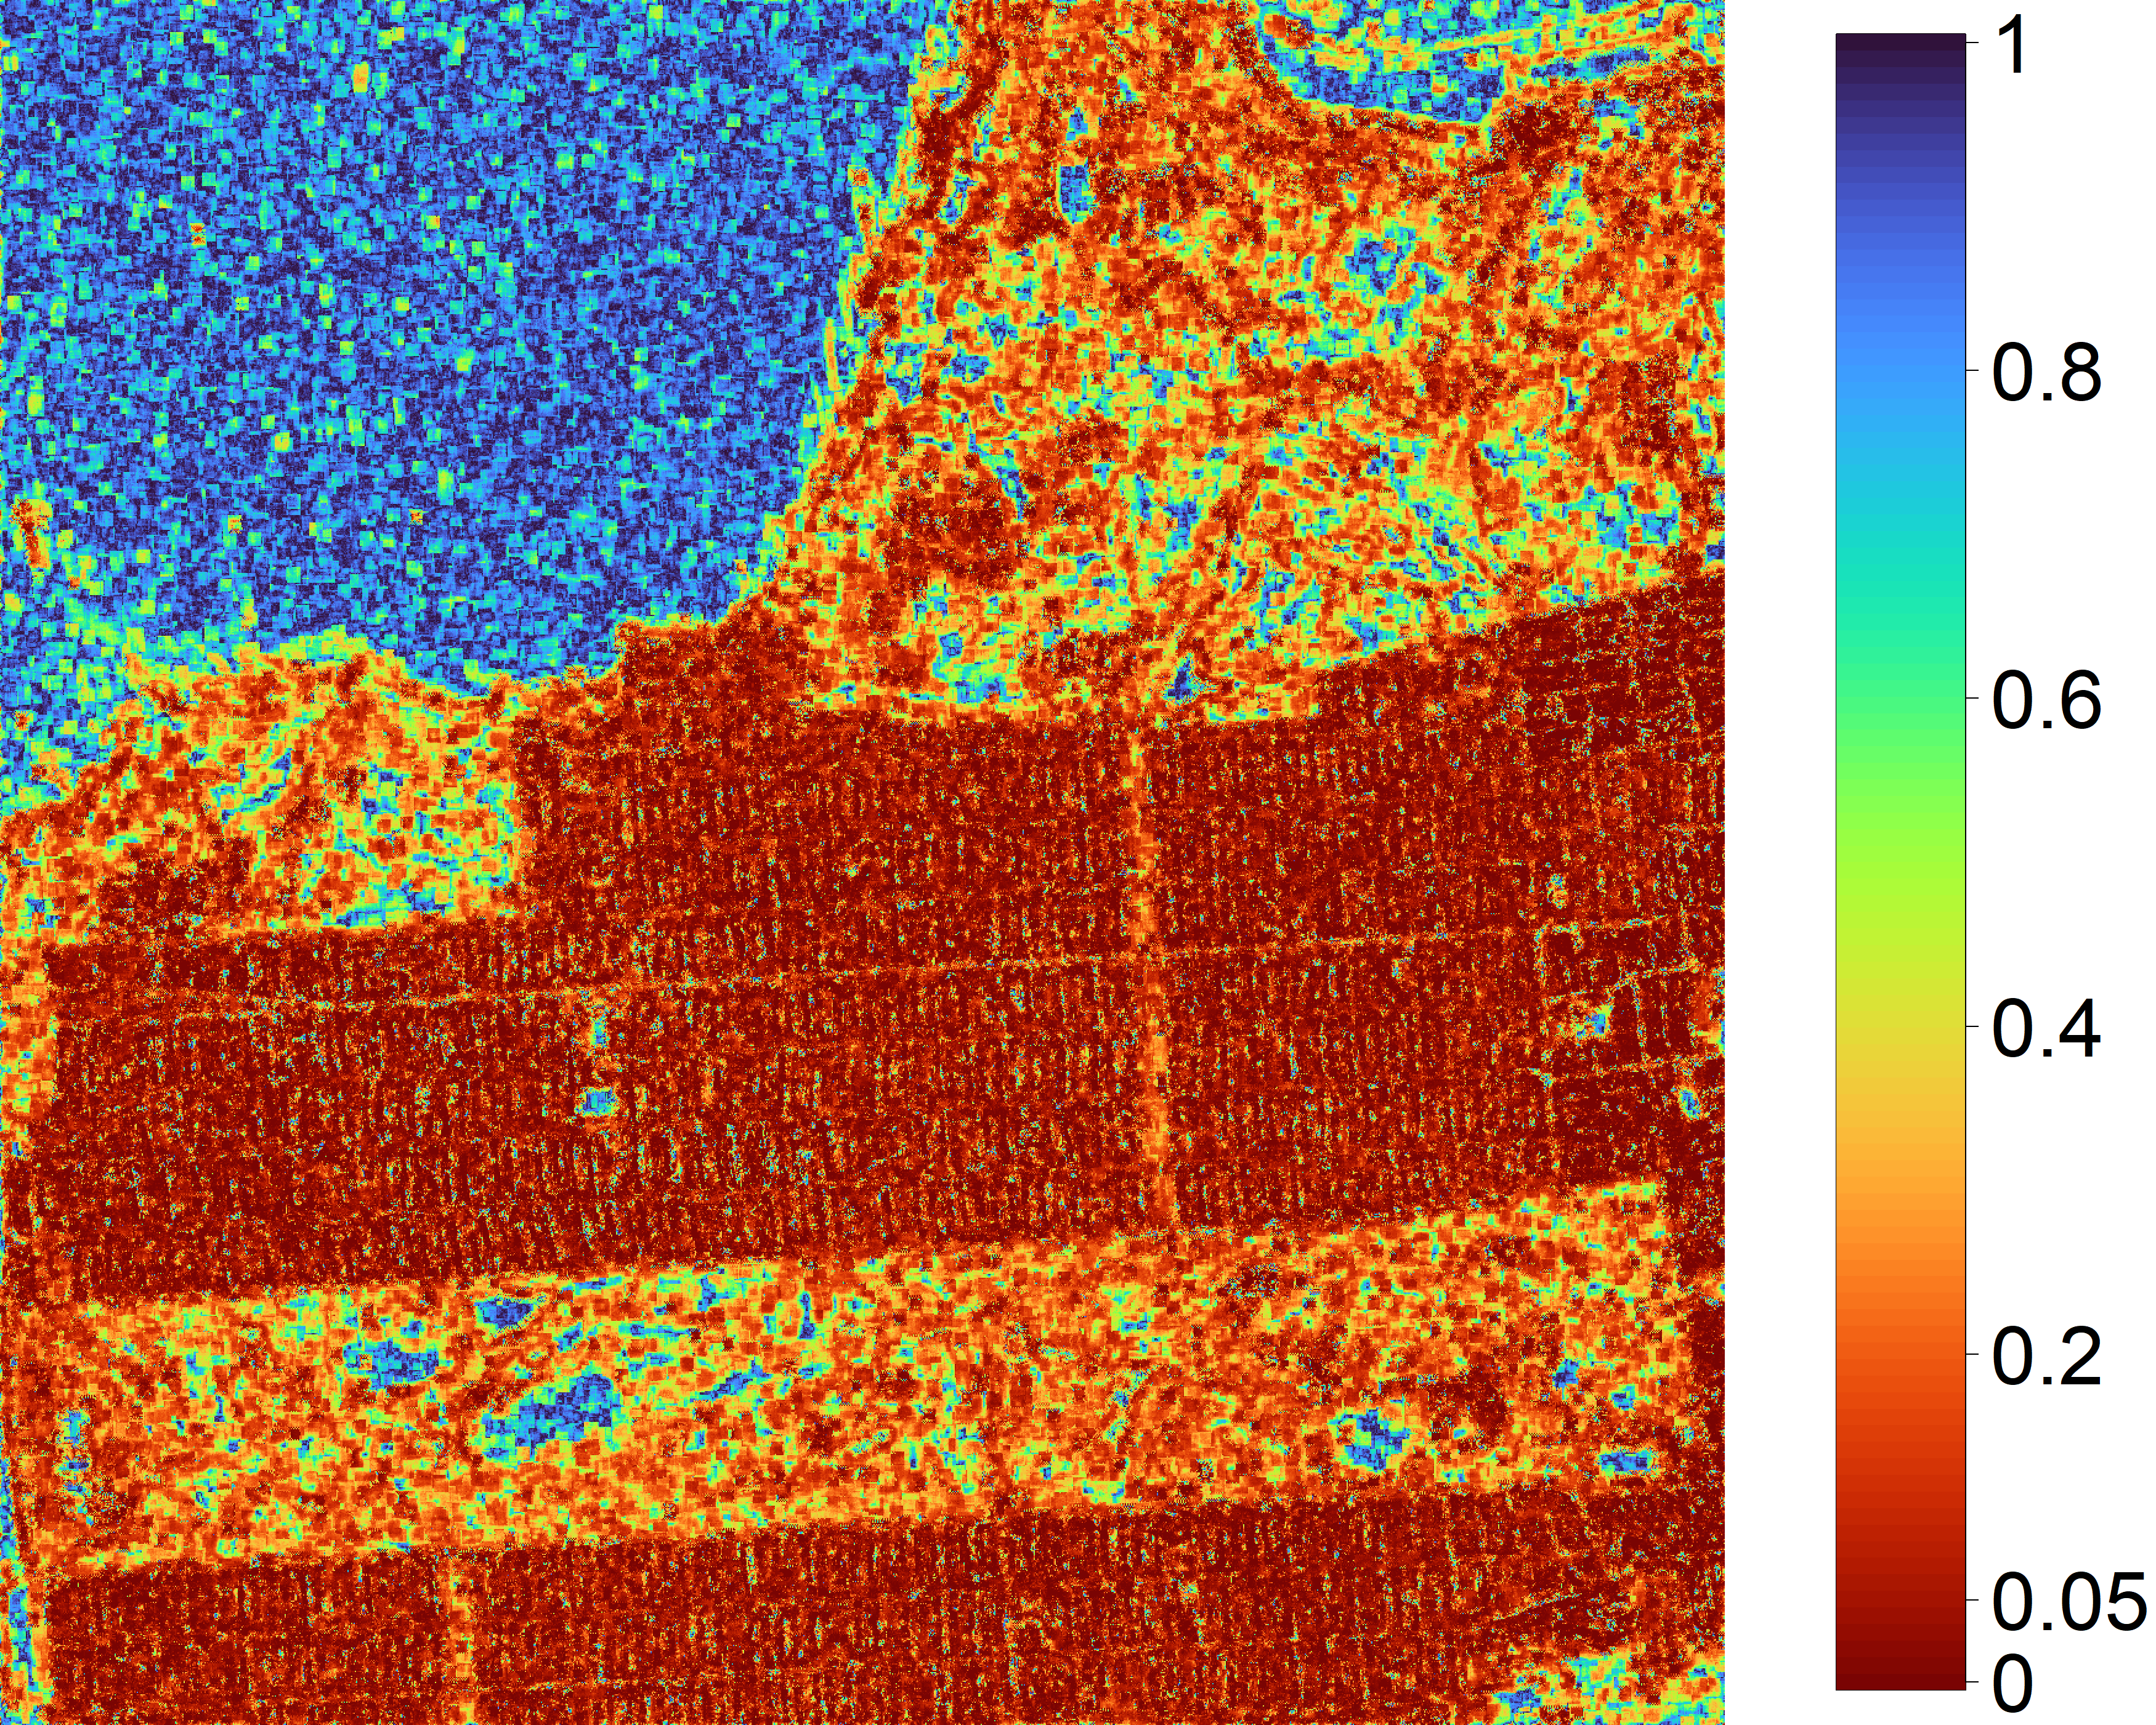
\includegraphics[width=\linewidth]{./Figures/p-values_San-fran1400_eta2_B100_lambda_085-5x11_L4_1.png}
\caption{$p$-value map ($\eta=2$)}
\label{fig:SFc3}
\end{subfigure}\hfill
\begin{subfigure}[t]{0.19\textwidth}
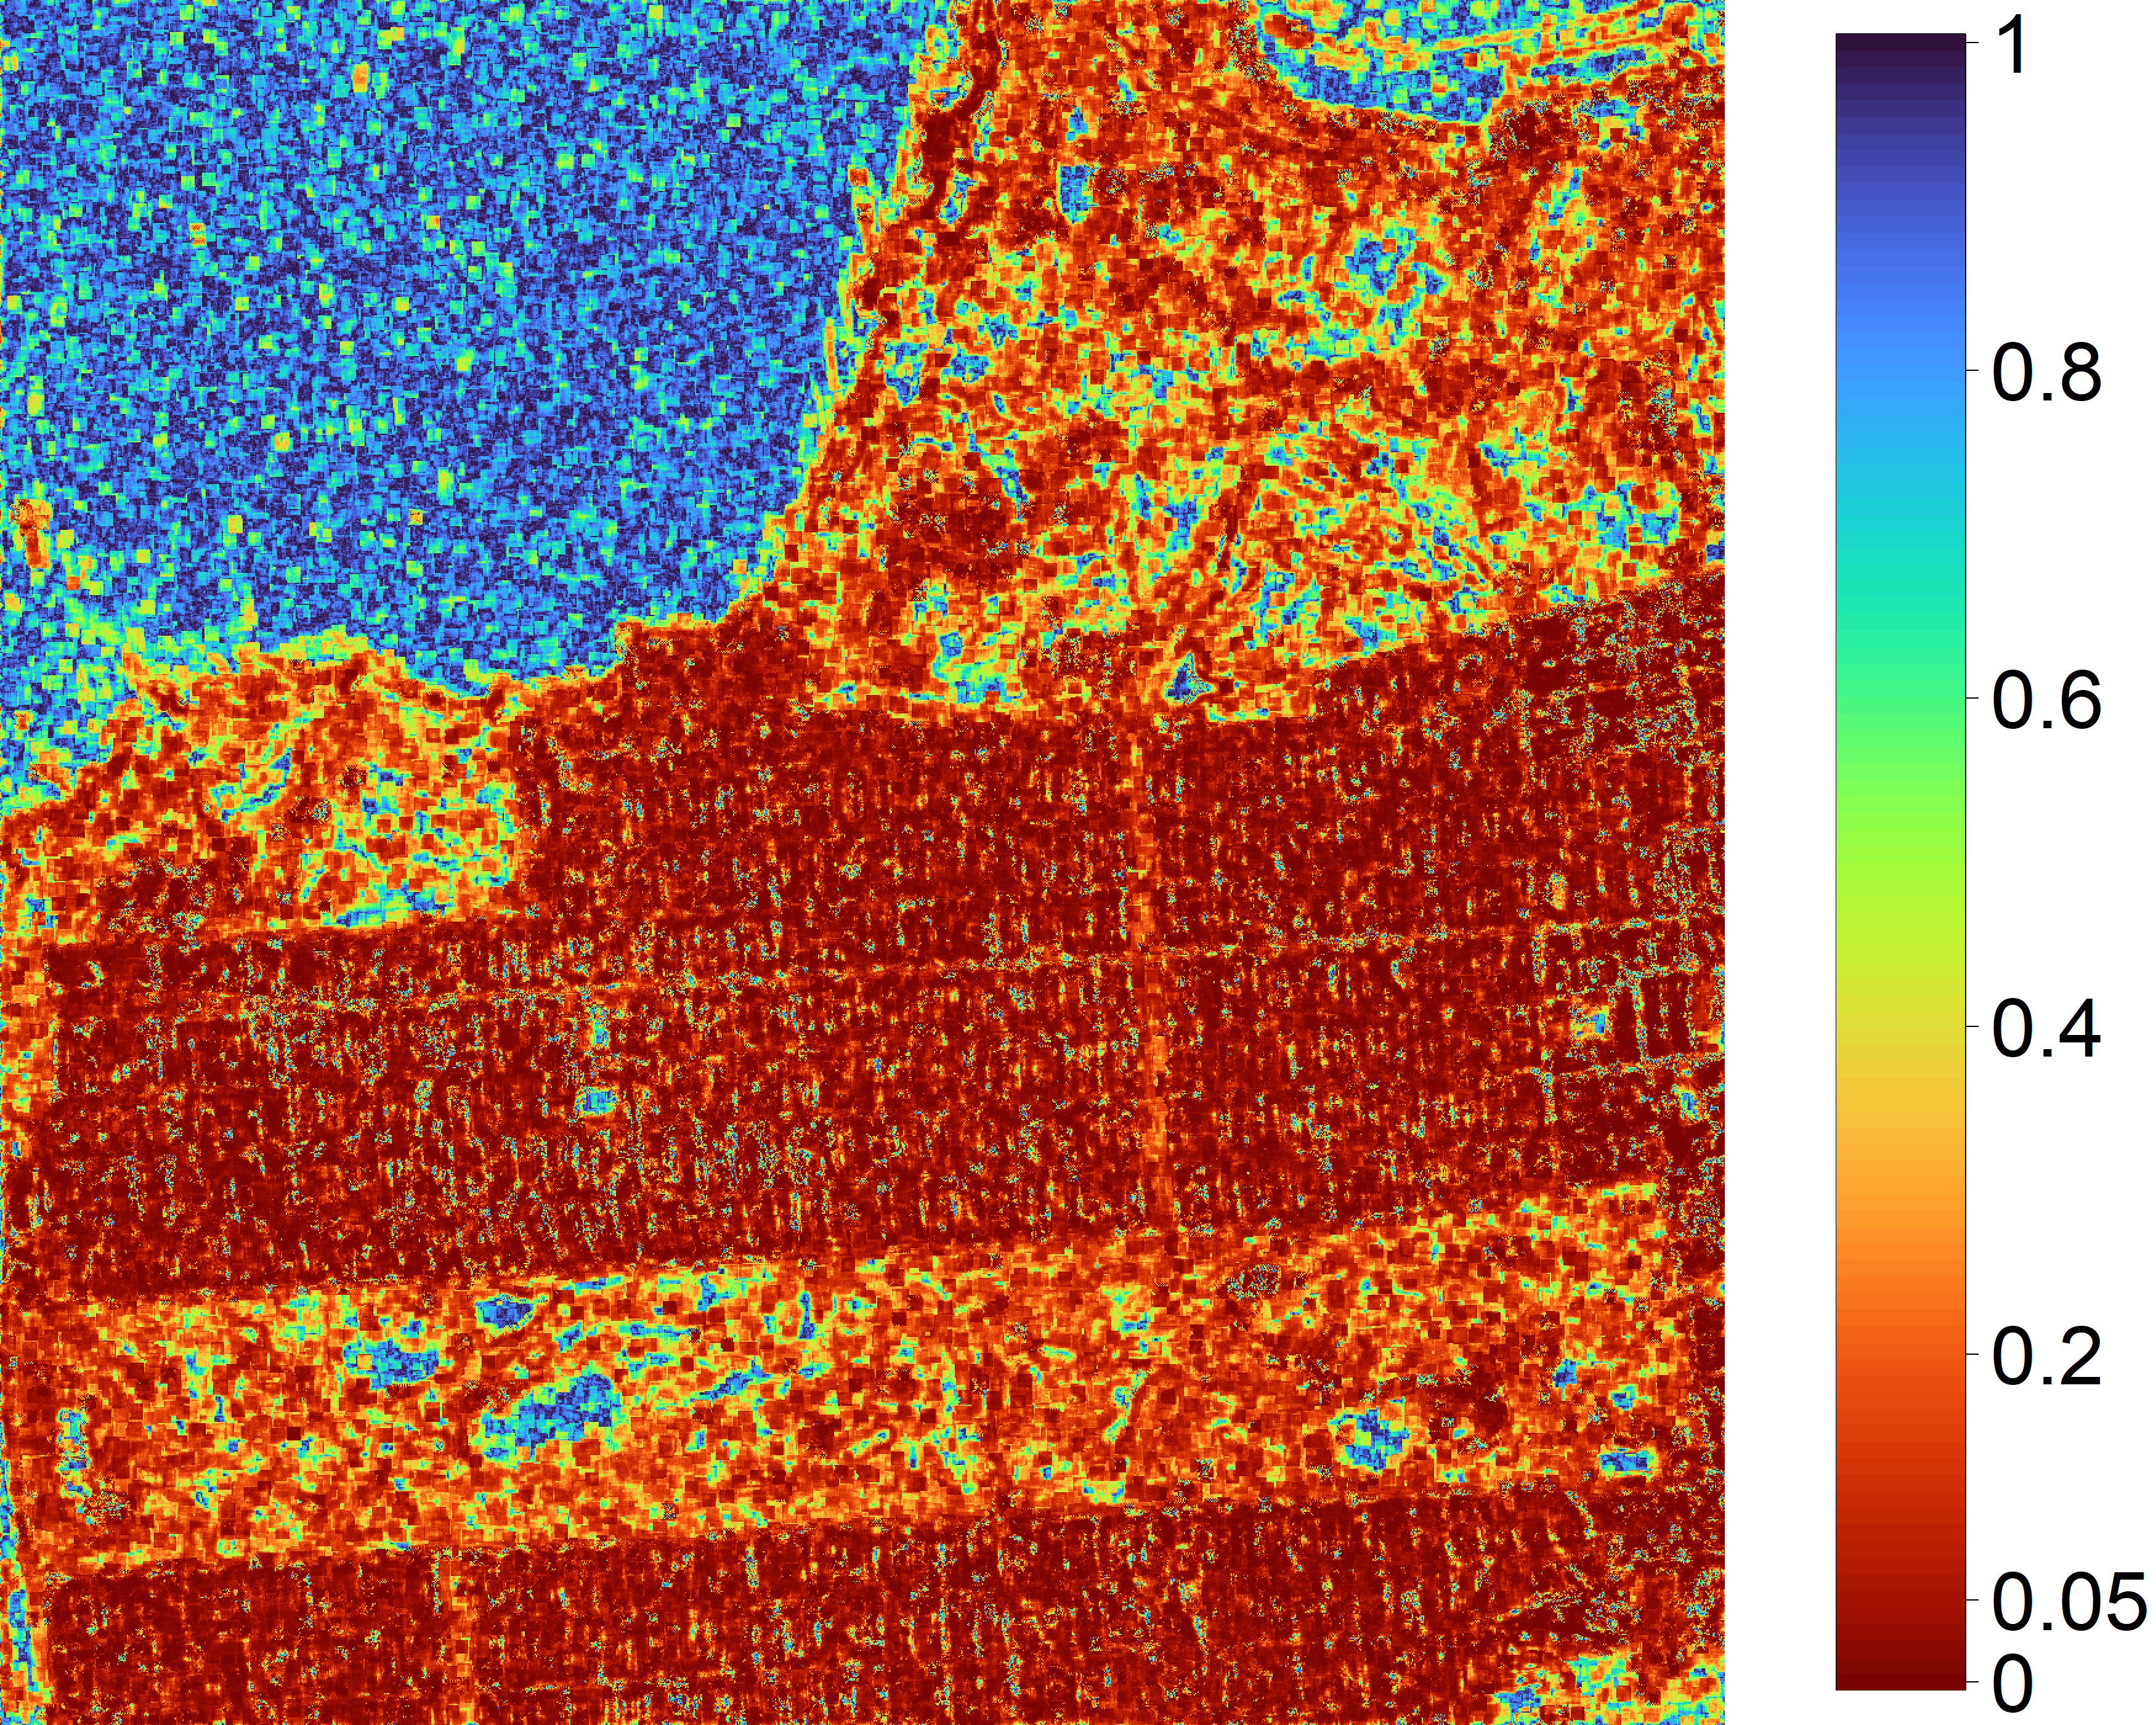
\includegraphics[width=\linewidth]{./Figures/p-values_San-fran1400_eta3_B100_lambda_085-5x11_L4_1.png}
\caption{$p$-value map ($\eta=3$)}
\label{fig:SFc4}
\end{subfigure}\hfill
\begin{subfigure}[t]{0.19\textwidth}
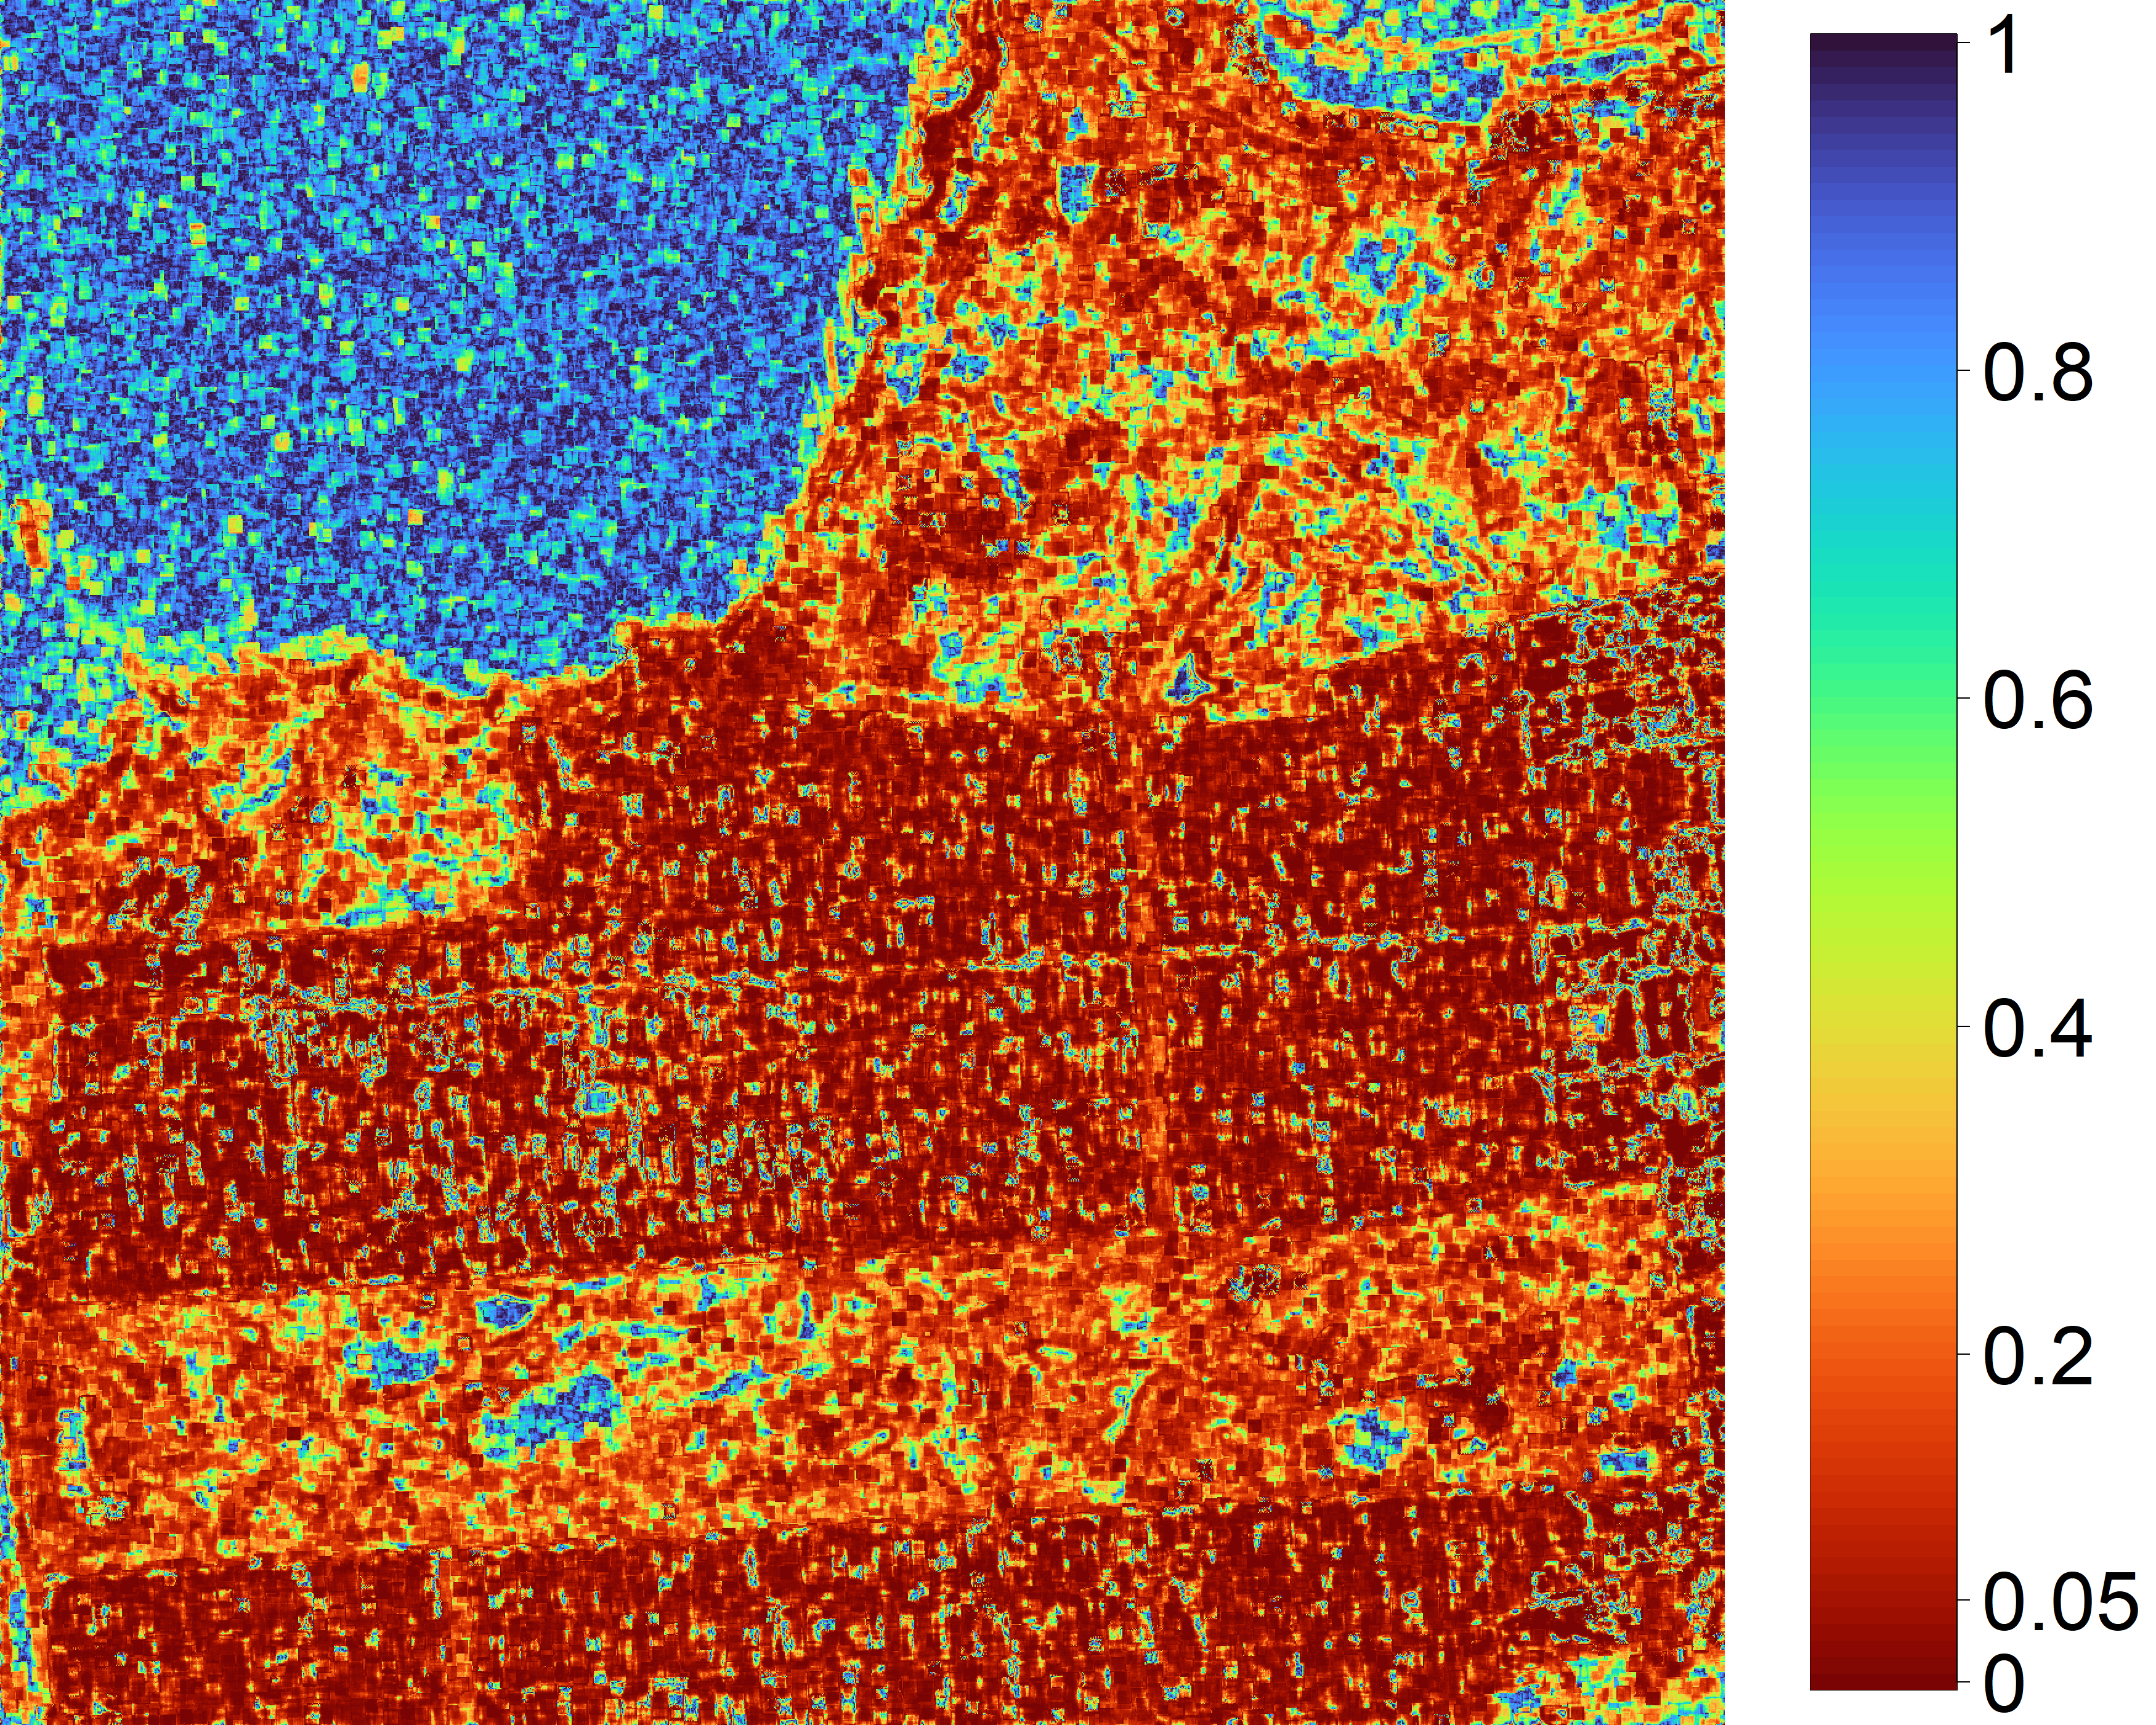
\includegraphics[width=\linewidth]{./Figures/p-values_San-fran1400-eta4.png} % (o deja esta vacía si solo tienes 4)
\caption{$p$-value map ($\eta=4$)}
\label{fig:SFc5}
\end{subfigure}

\vspace{4pt} % separa filas (ajusta si hace falta)

\begin{subfigure}[t]{0.18\textwidth}
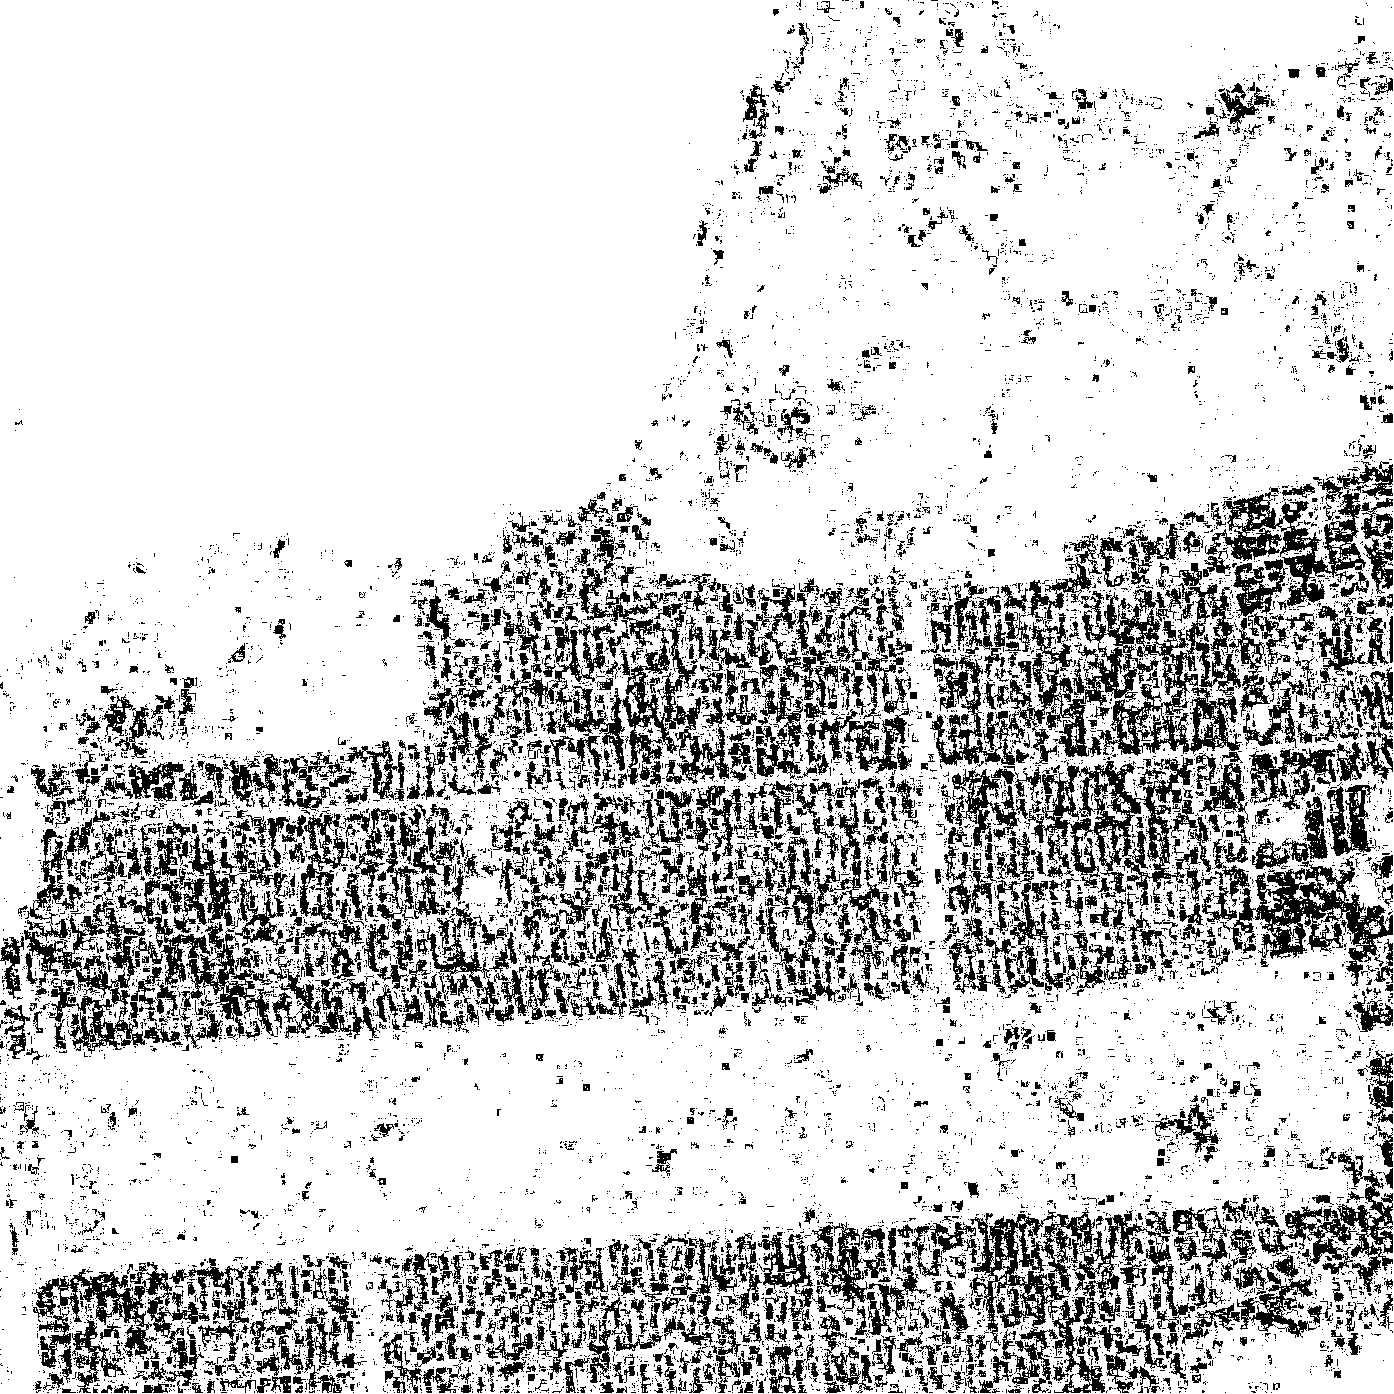
\includegraphics[width=\linewidth]{./Figures/H_005_SF_7x7.png}
\caption{Binary map ($7\times7$)}
\label{fig:SFbc1}
\end{subfigure}\hfill
\begin{subfigure}[t]{0.18\textwidth}
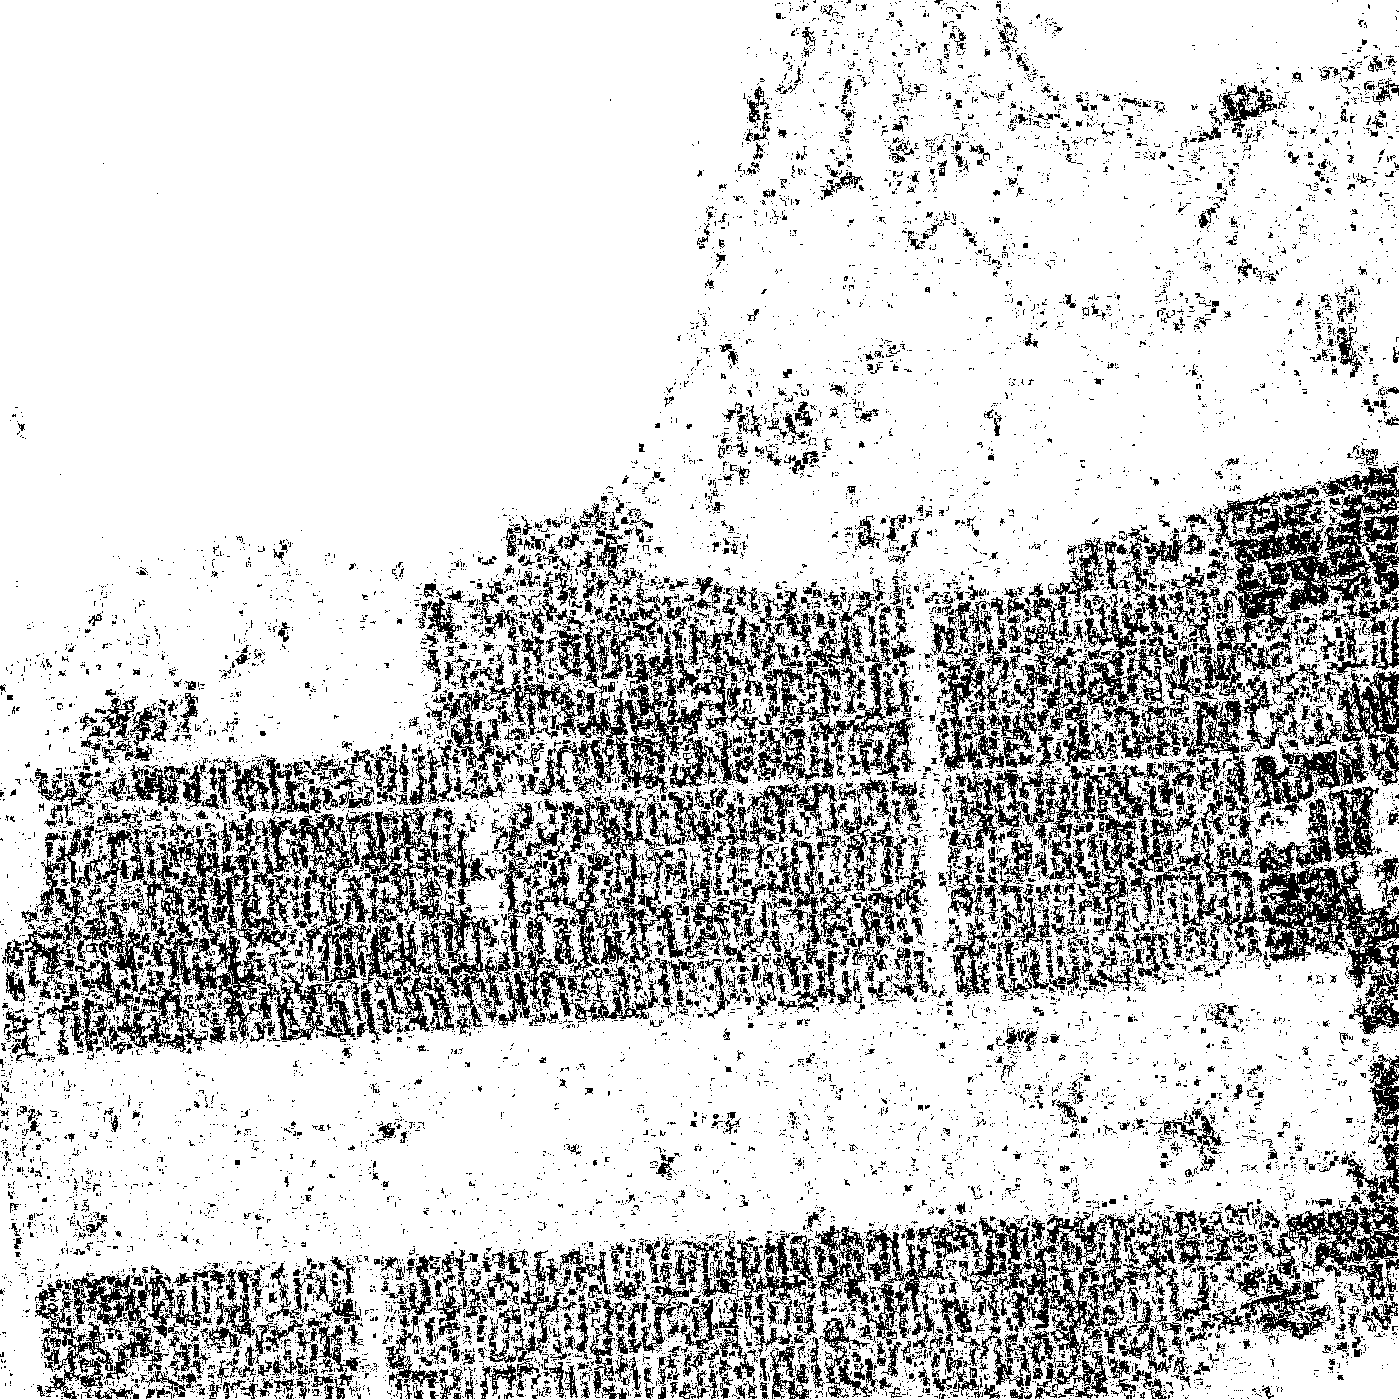
\includegraphics[width=\linewidth]{./Figures/H_005_San-fran1400_eta1_B100_lambda_085-5x11_L4_1.png}
\caption{Binary map ($\eta=1$)}
\label{fig:SFbc2}
\end{subfigure}\hfill
\begin{subfigure}[t]{0.18\textwidth}
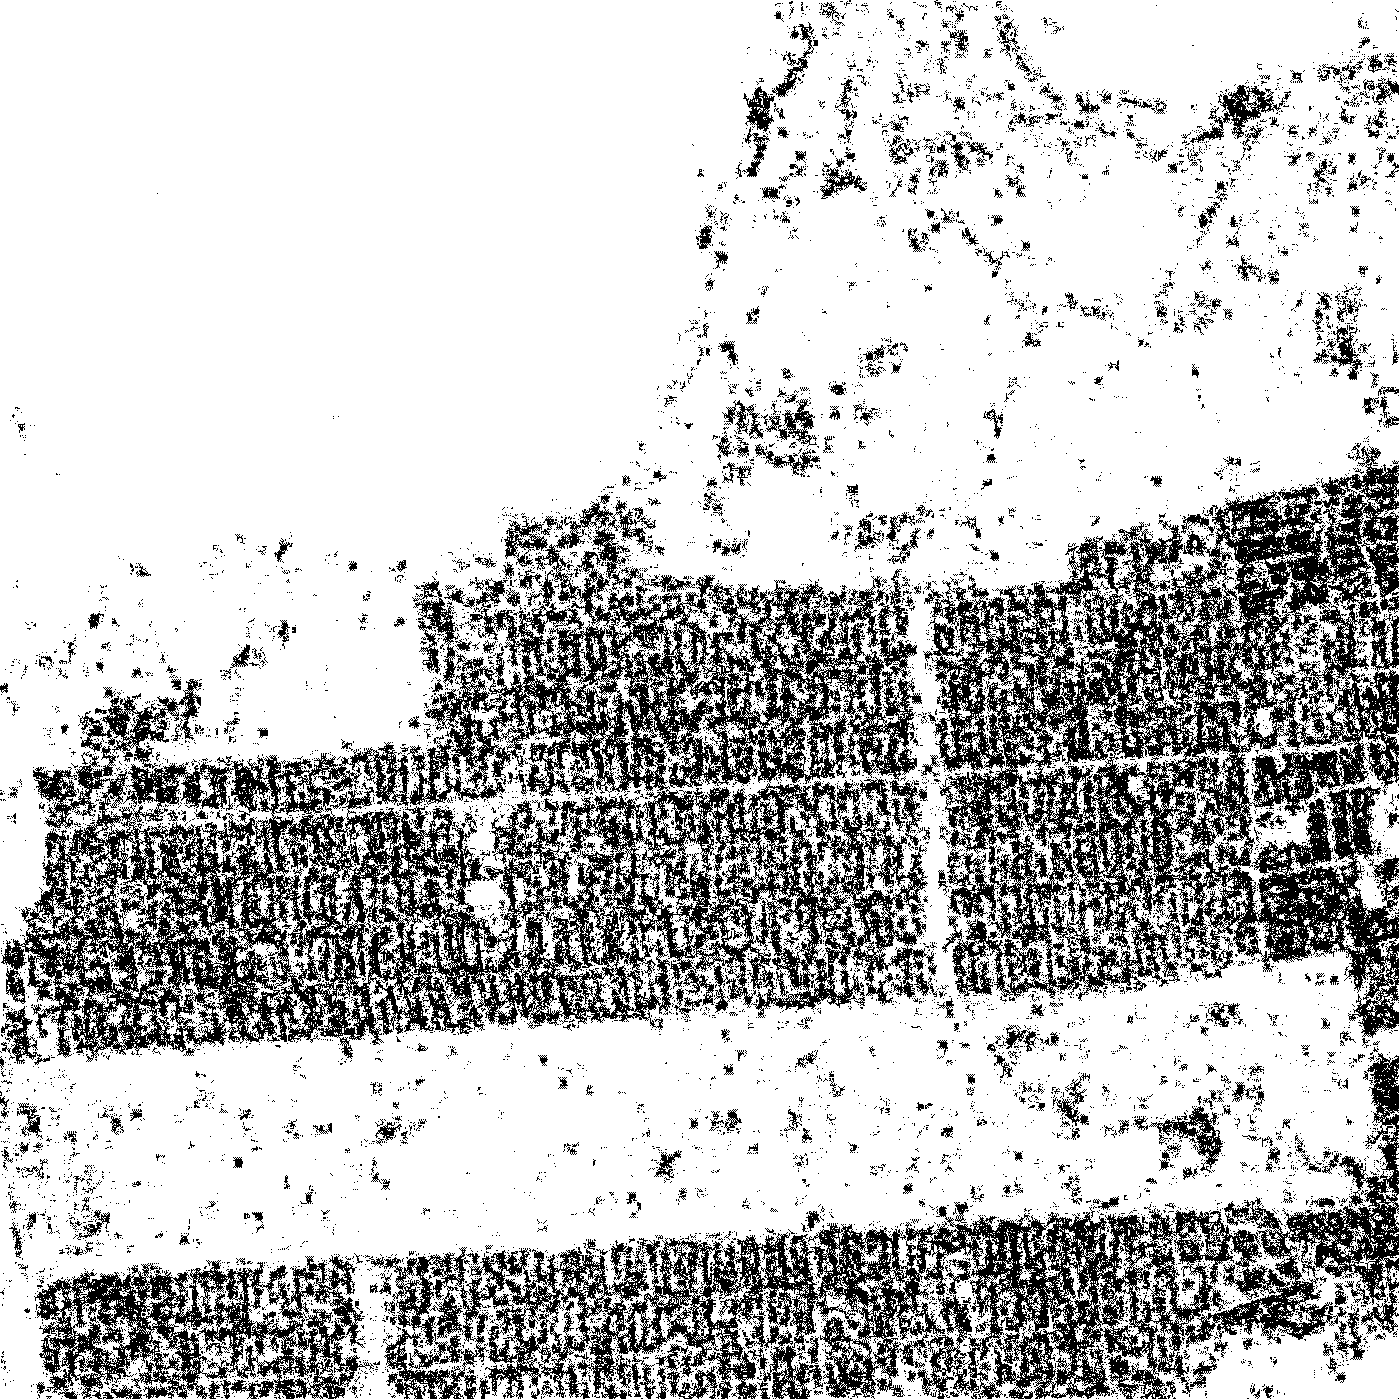
\includegraphics[width=\linewidth]{./Figures/H_005_San-fran1400_eta2_B100_lambda_085-5x11_L4_1.png}
\caption{Binary map ($\eta=2$)}
\label{fig:SFbc3}
\end{subfigure}\hfill
\begin{subfigure}[t]{0.18\textwidth}
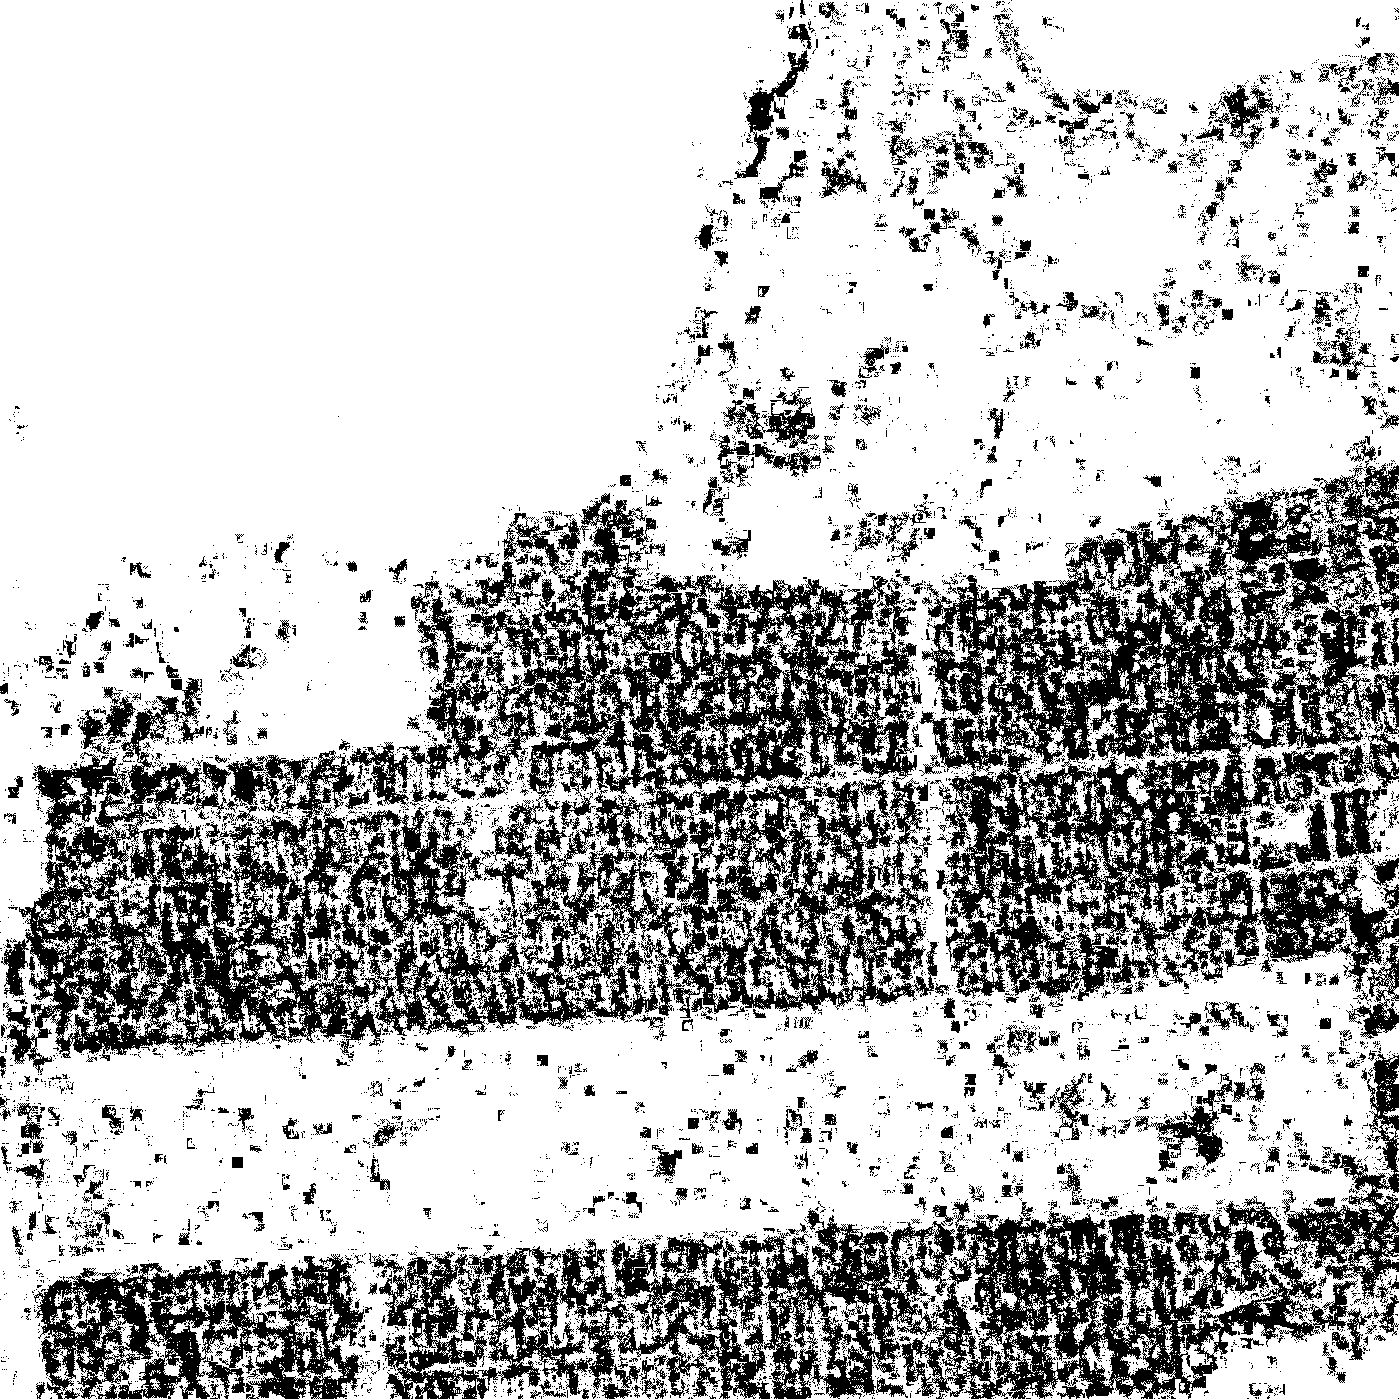
\includegraphics[width=\linewidth]{./Figures/H_005_San-fran1400_eta3_B100_lambda_085-5x11_L4.png}
\caption{Binary map ($\eta=3$)}
\label{fig:SFbc4}
\end{subfigure}\hfill
\begin{subfigure}[t]{0.18\textwidth}
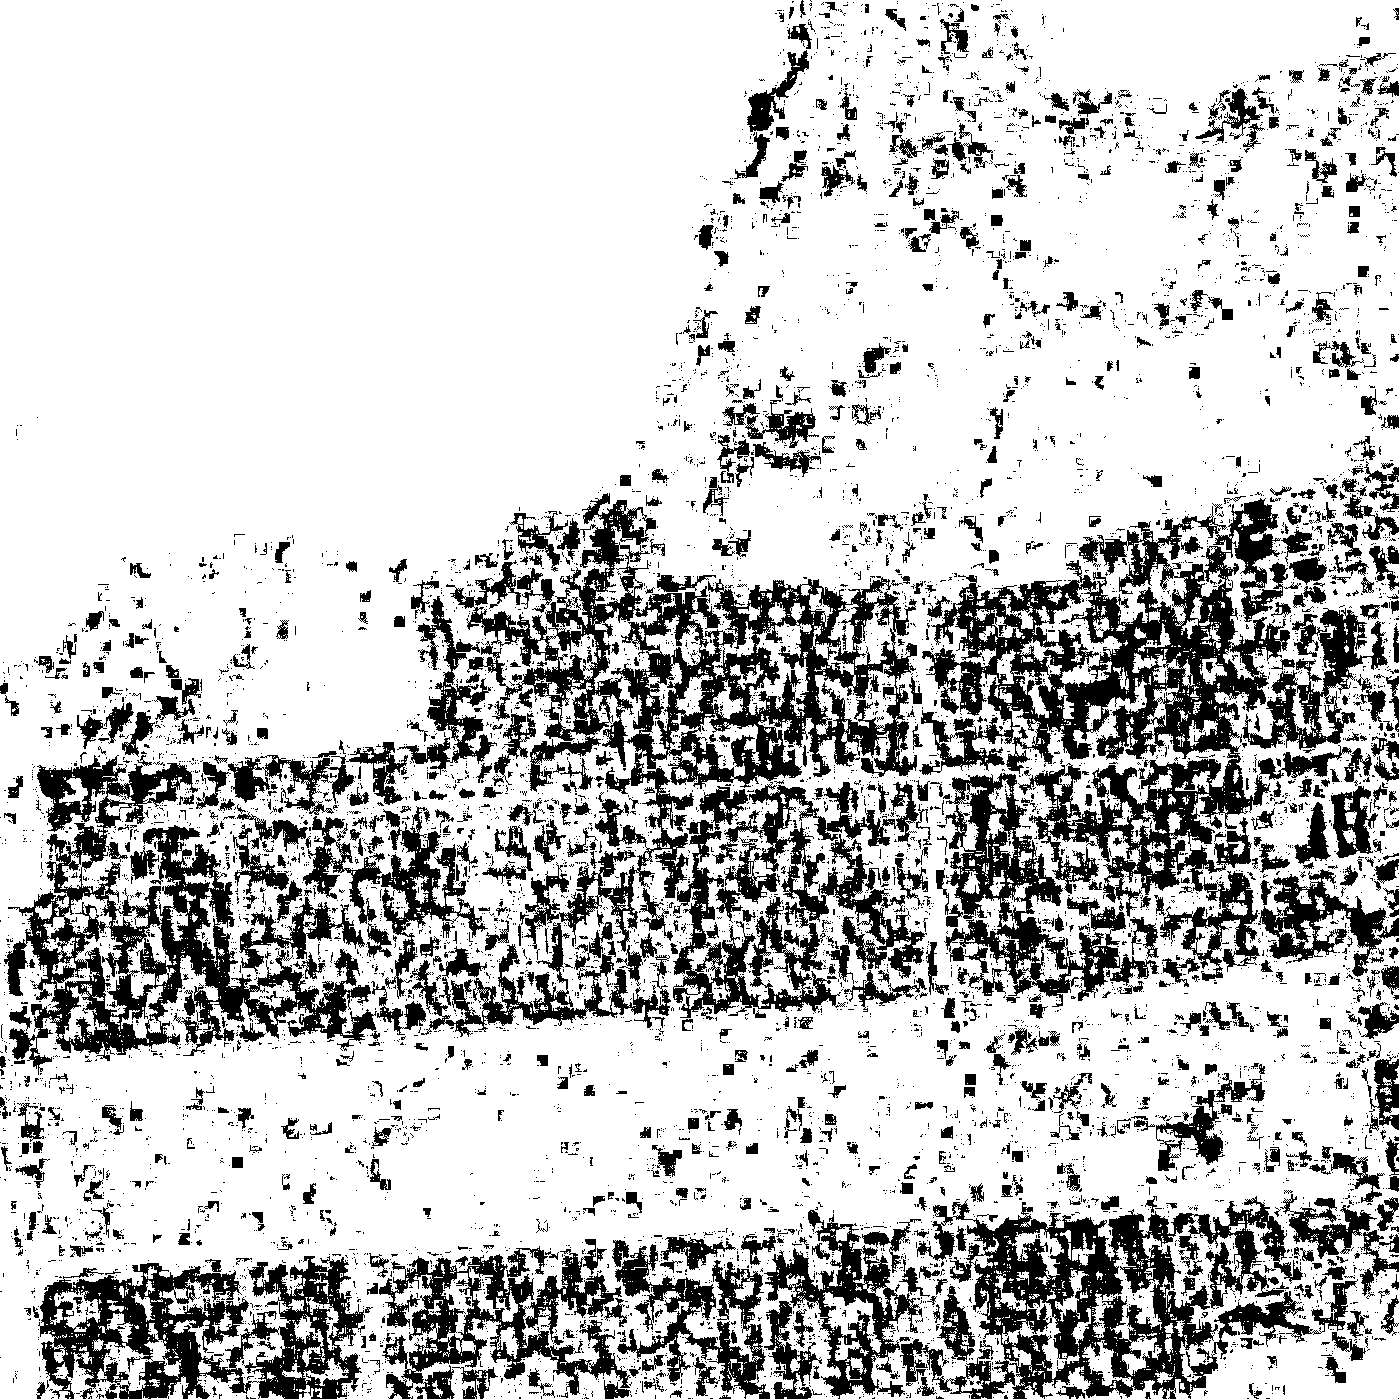
\includegraphics[width=\linewidth]{./Figures/H_005_San-fran_eta4.png}
\caption{Binary map  ($\eta=4$)}
\label{fig:SFbc5}
\end{subfigure}
\caption{Detection of heterogeneous areas in a SAR image over San Francisco. 
(a) $p$-value map with a fixed $7\times7$ window.
(b–e) $p$-value maps with adaptive windows ($W_{\min}=5$, $W_{\max}=11$) for
$\eta=1$--$4$. (f--j) Binary decision maps at $0.05$ significance level.}
\label{fig:sanfrancisco}
\end{figure*}

\begin{figure*}[!t]
\centering
\captionsetup{font=footnotesize}
\captionsetup[sub]{aboveskip=2pt,belowskip=2pt}

\begin{subfigure}[t]{0.19\textwidth}
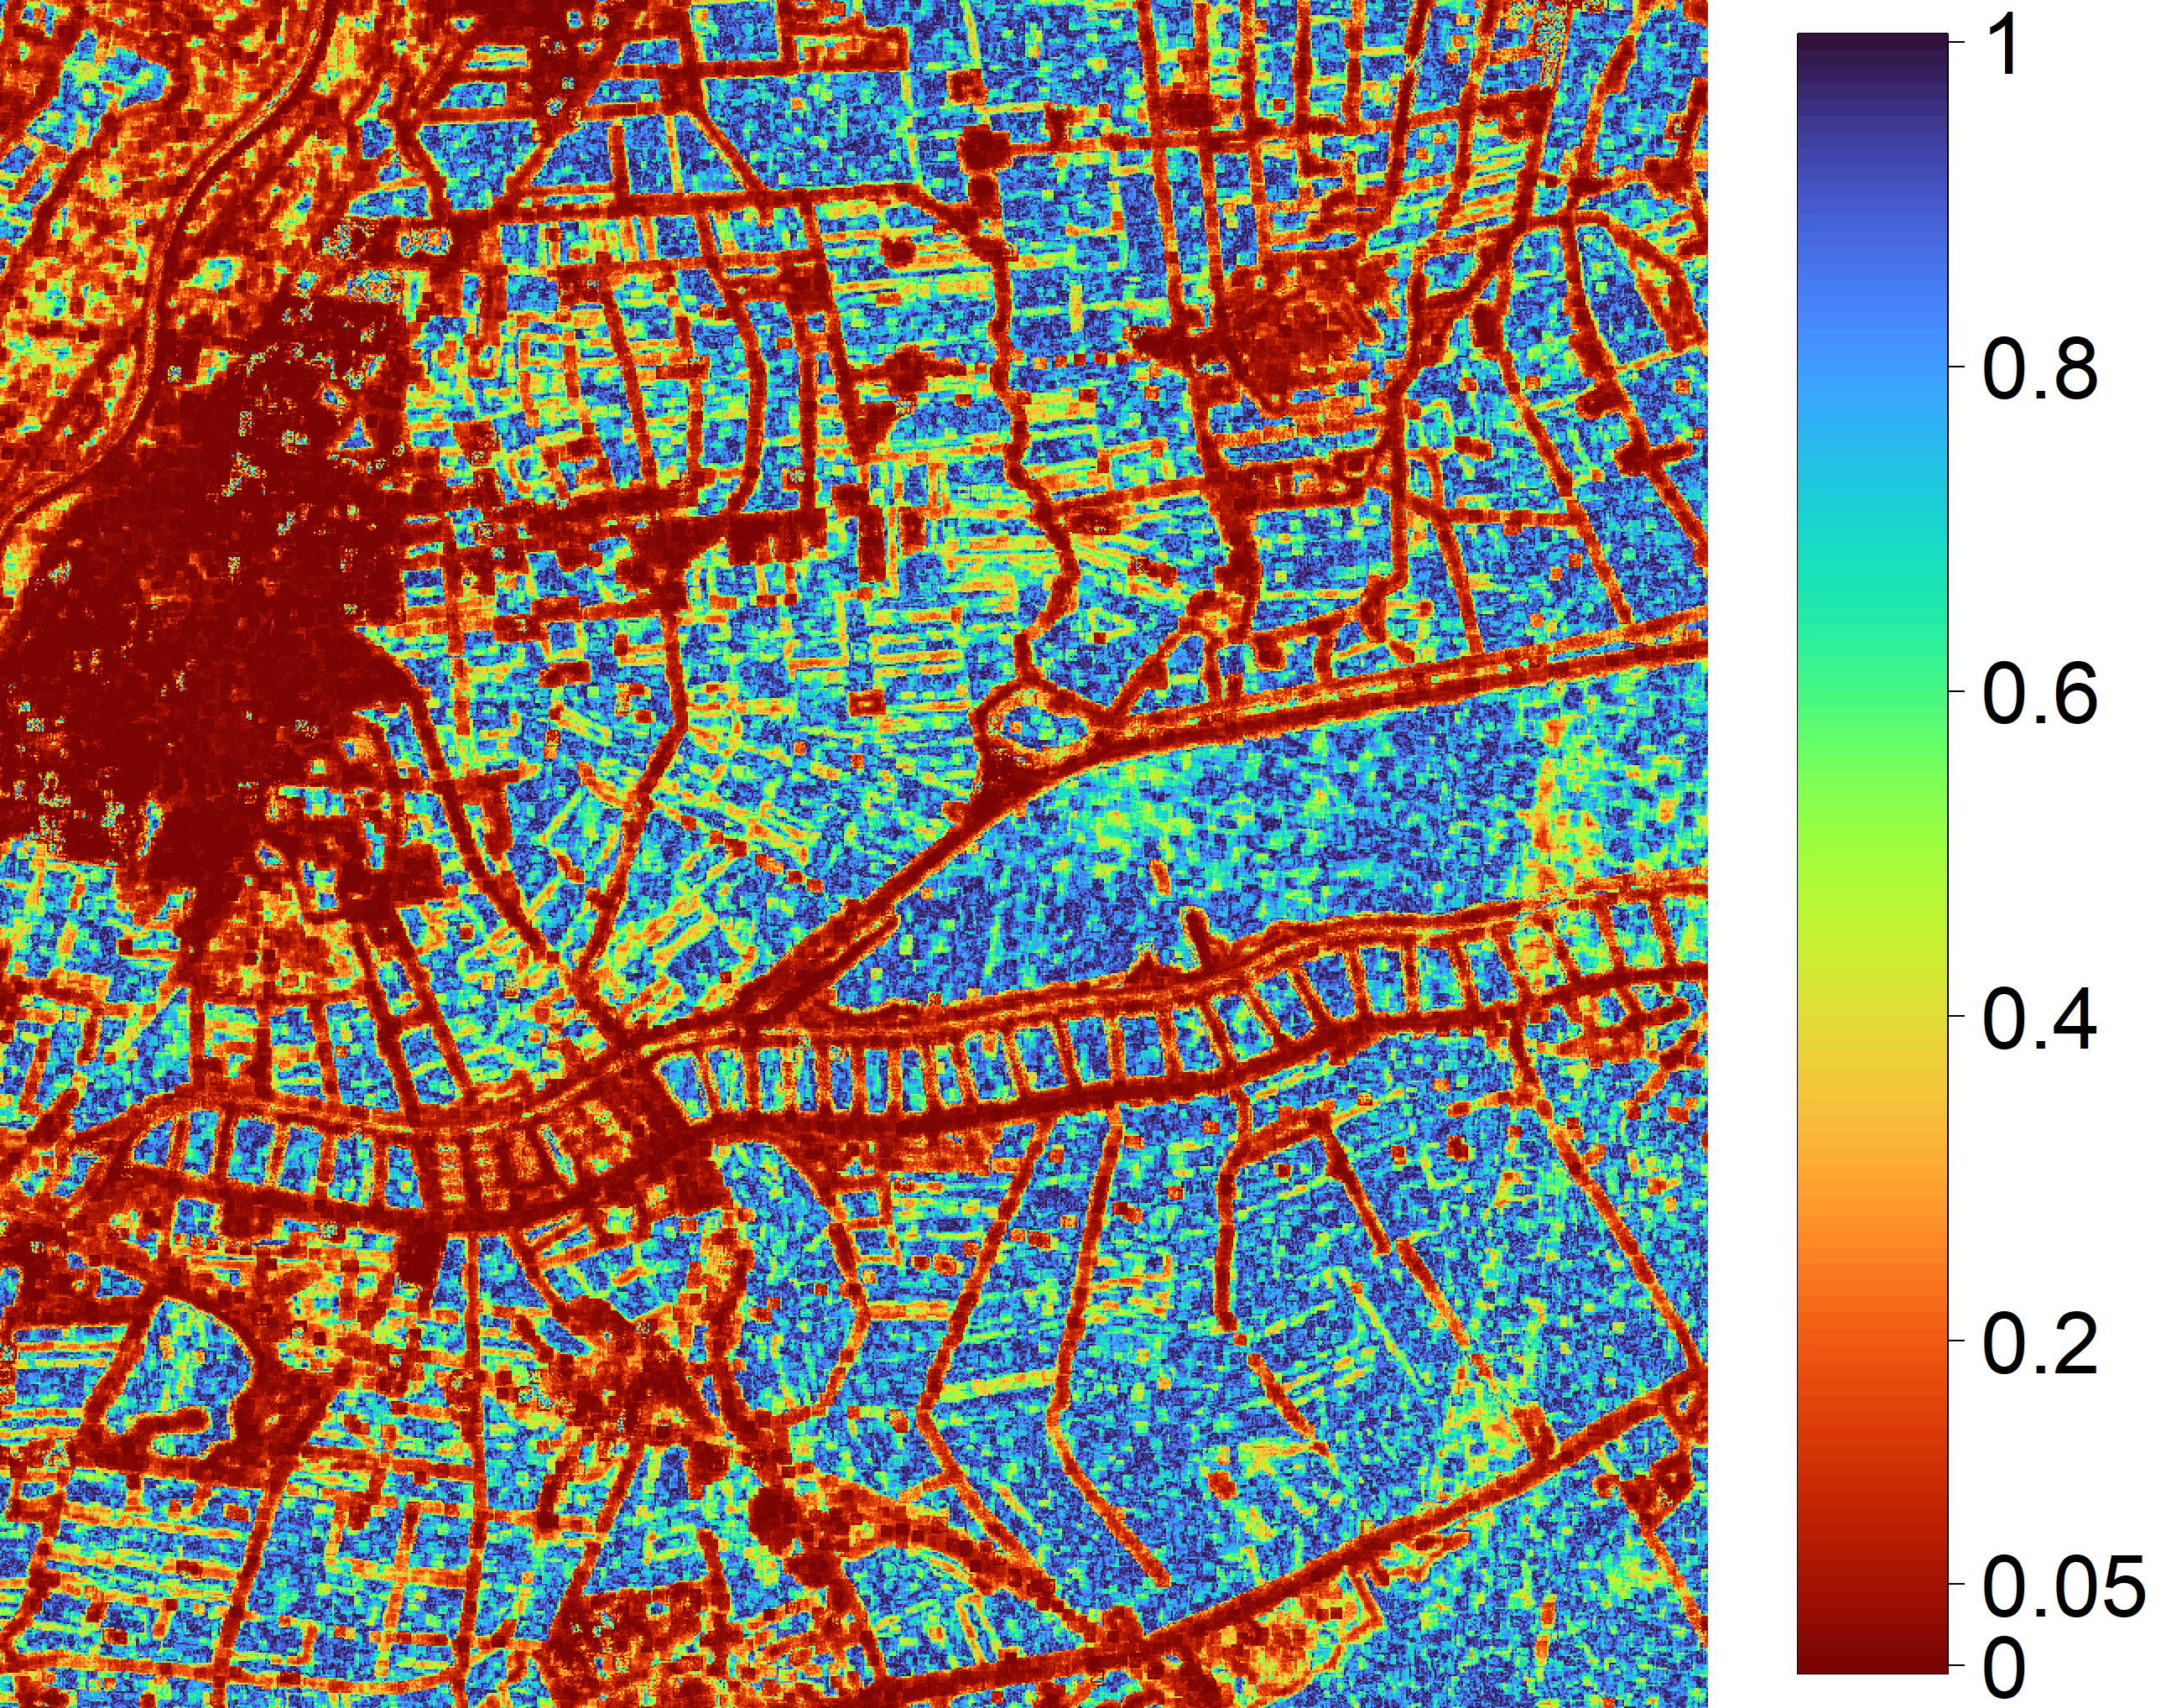
\includegraphics[width=\linewidth]{./Figures/p-values_munich1024_lambda085_7x7.png}
\caption{$p$-value map ($7\times7$)}
\label{fig:muc1}
\end{subfigure}\hfill
\begin{subfigure}[t]{0.19\textwidth}
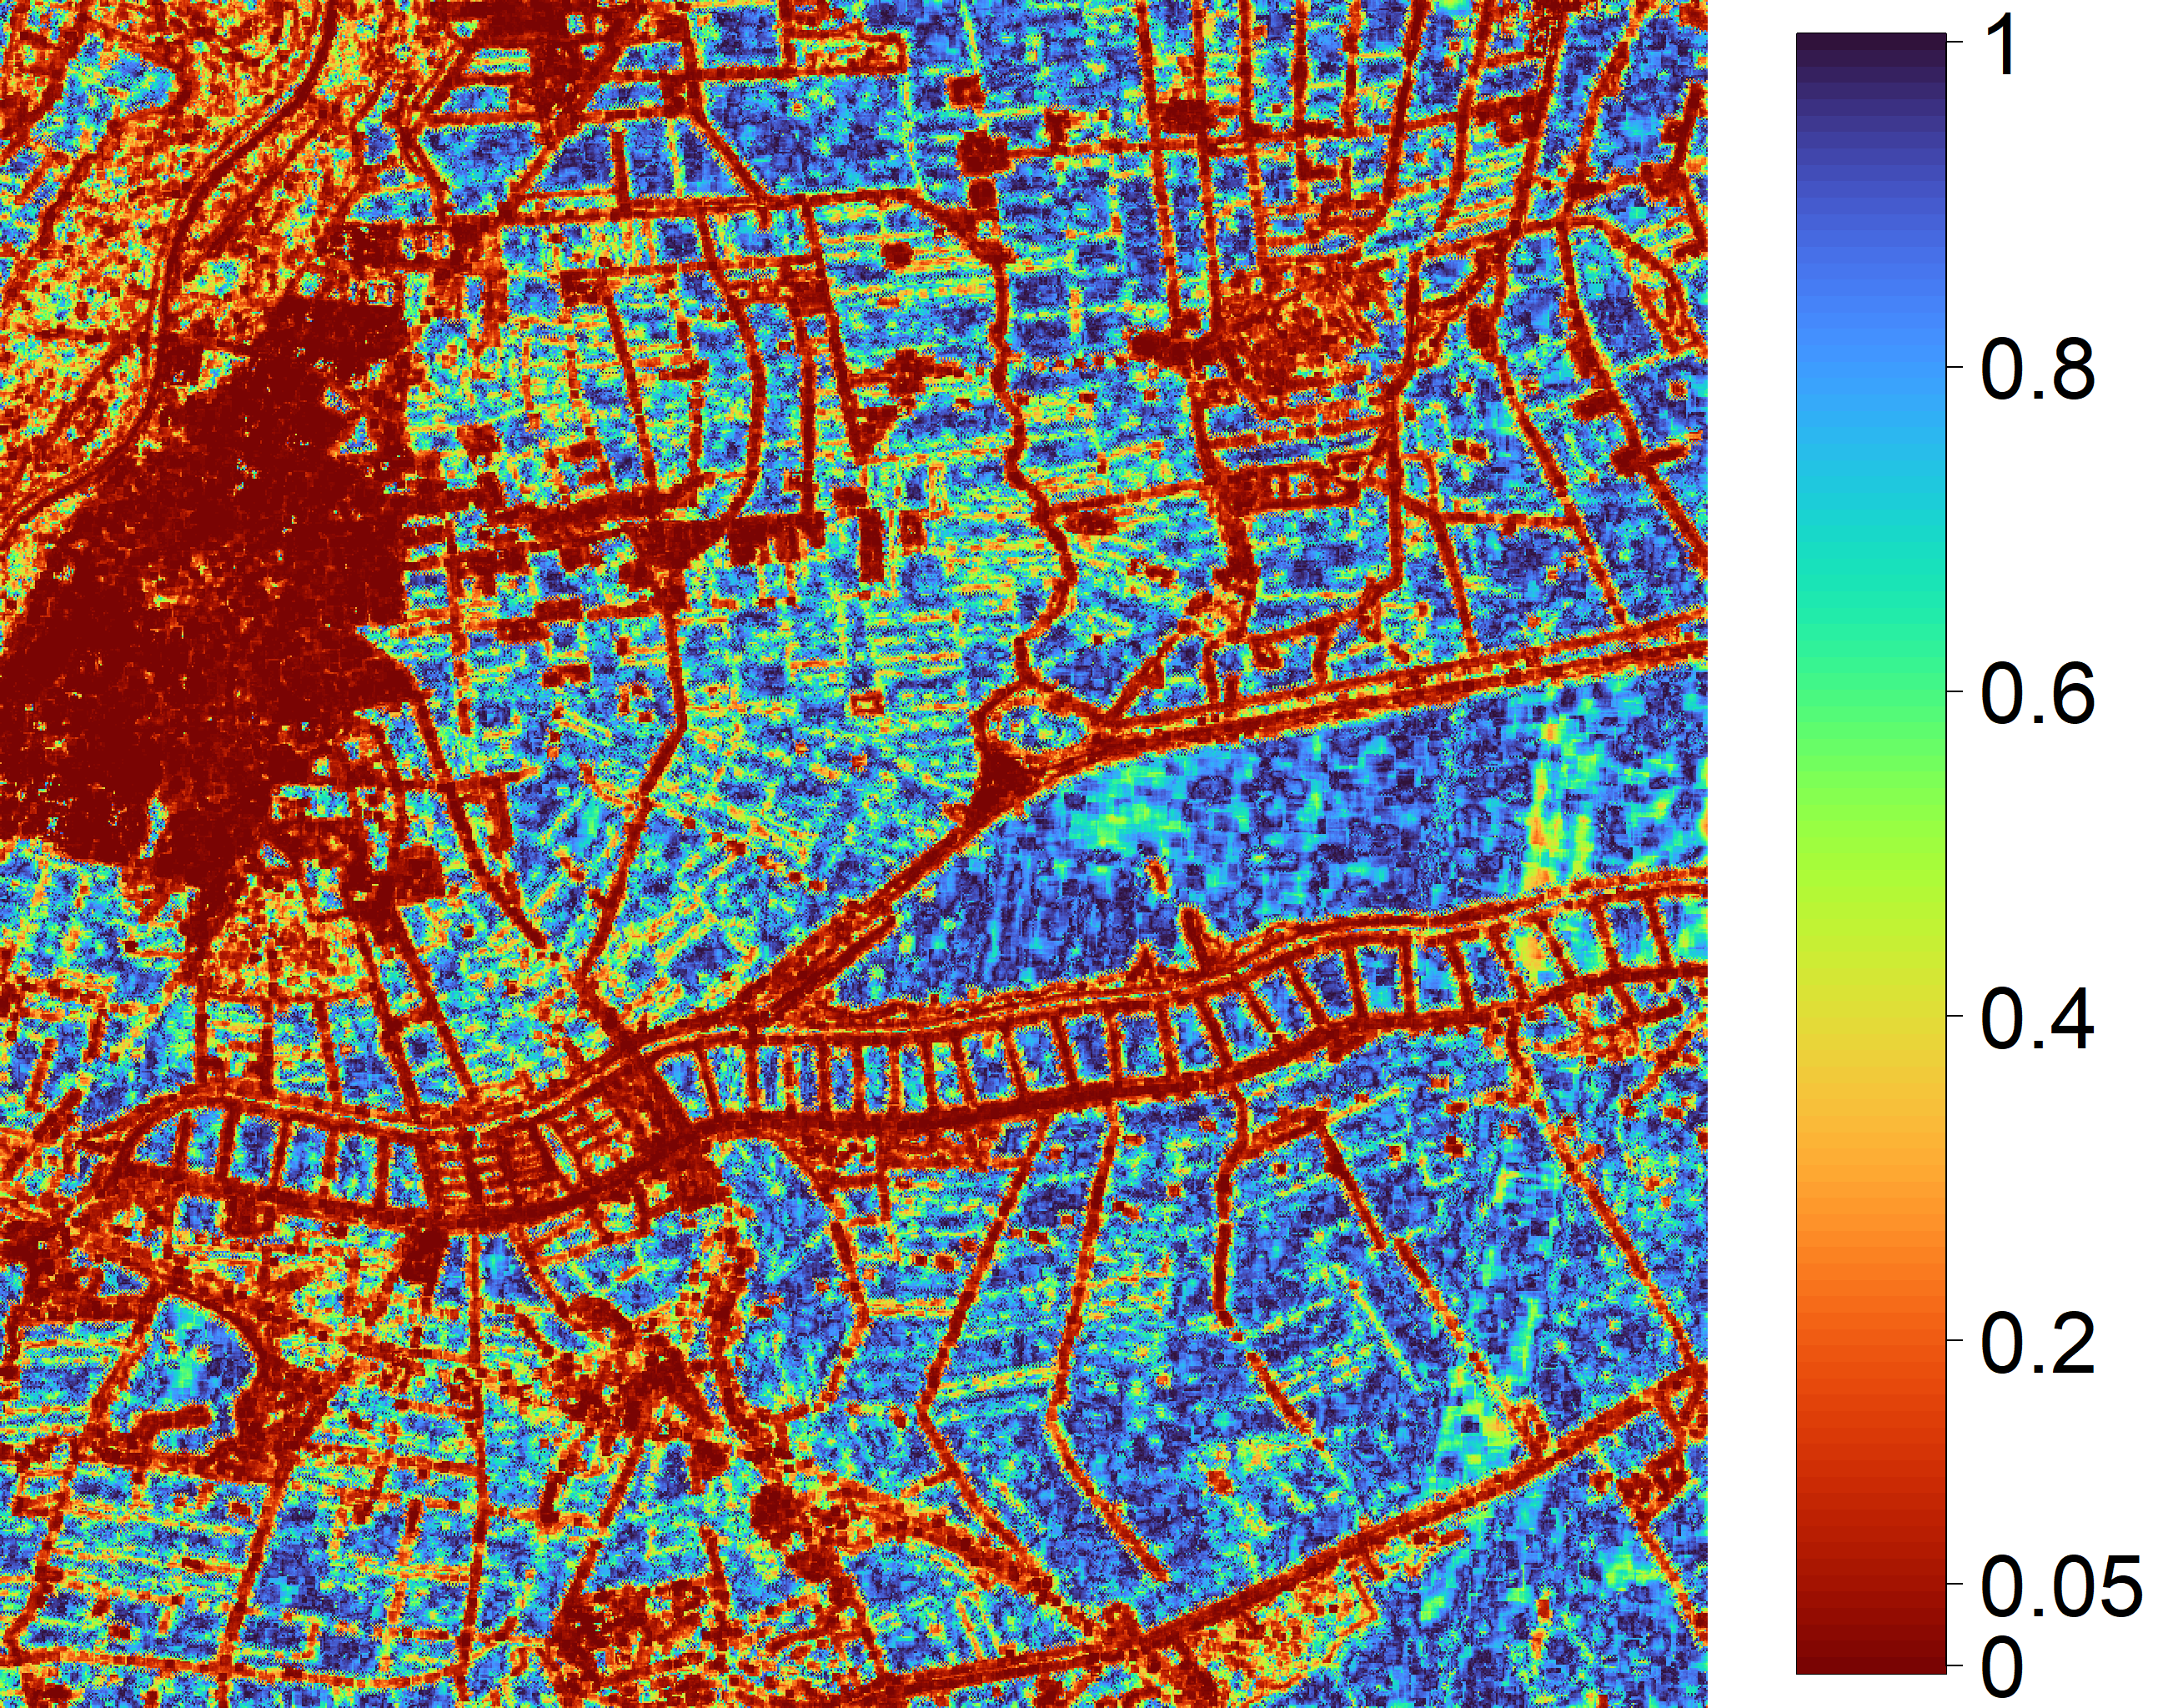
\includegraphics[width=\linewidth]{./Figures/p-values_munich1024_eta1.0_lambda085_5x11_b100.png}
\caption{$p$-value map ($\eta=1$)}
\label{fig:muc2}
\end{subfigure}\hfill
\begin{subfigure}[t]{0.19\textwidth}
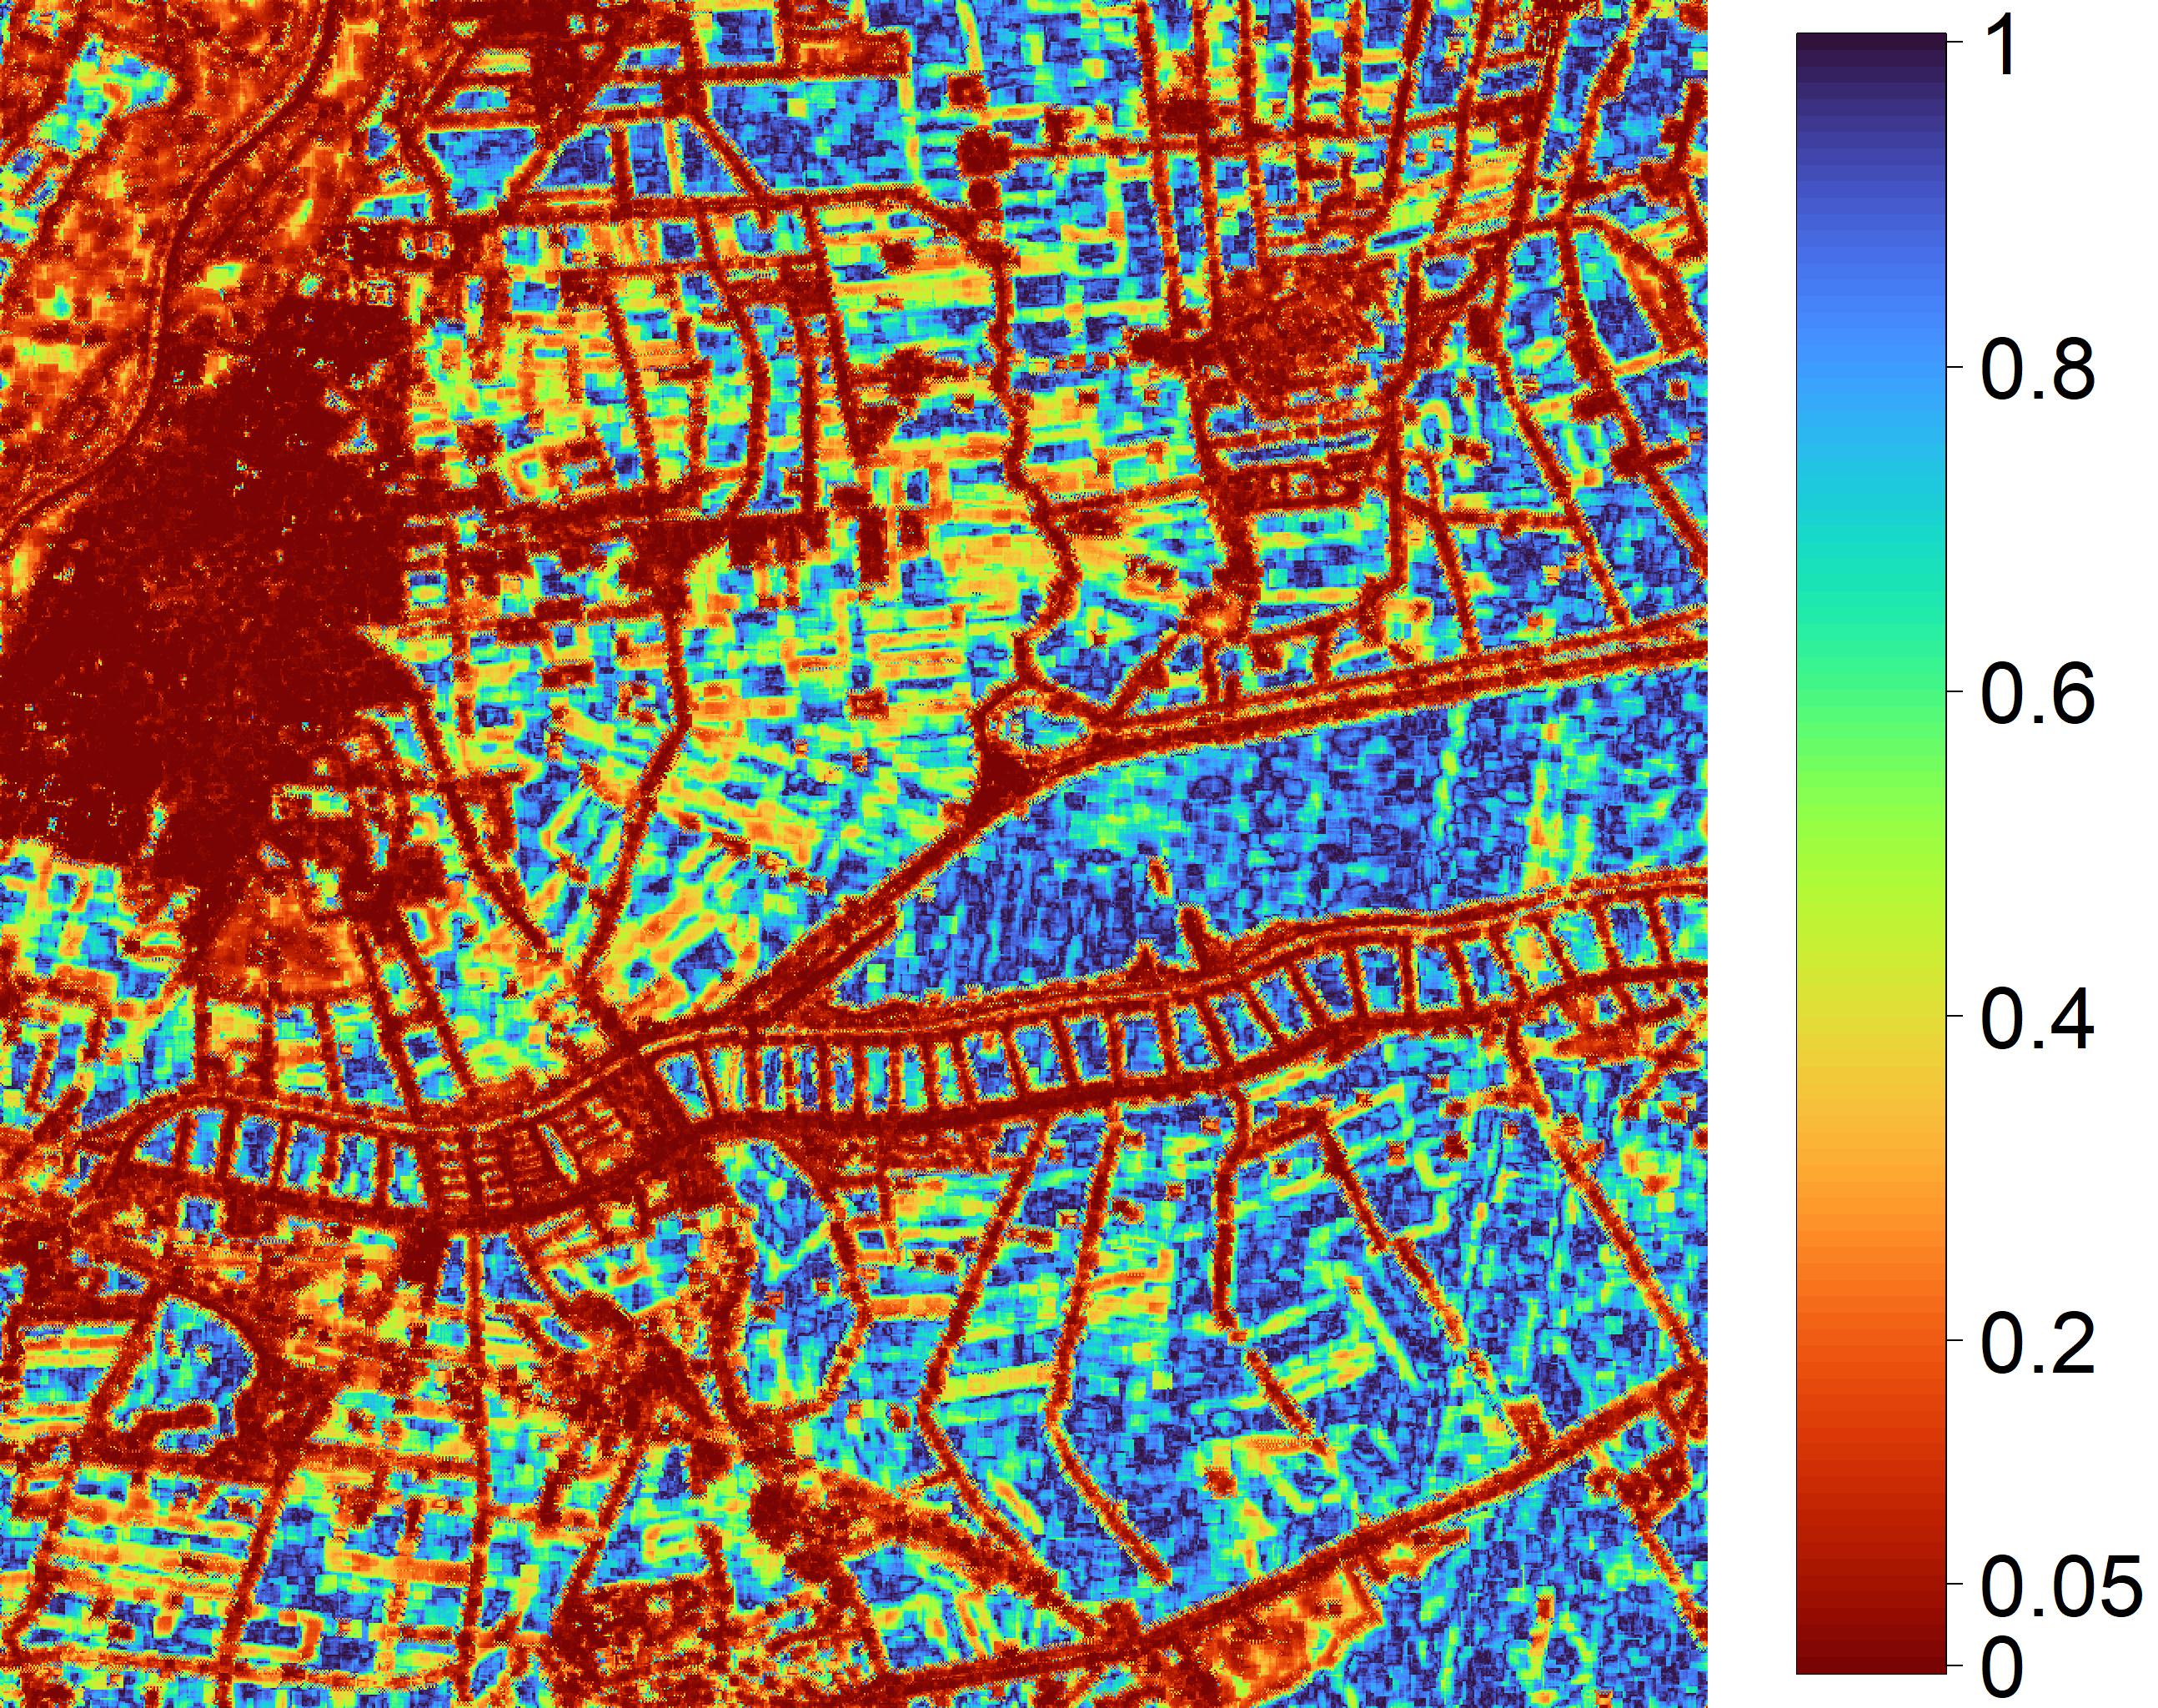
\includegraphics[width=\linewidth]{./Figures/p-values_munich1024_eta2.0_lambda085_5x11_b100.png}
\caption{$p$-value map ($\eta=2$)}
\label{fig:muc3}
\end{subfigure}\hfill
\begin{subfigure}[t]{0.19\textwidth}
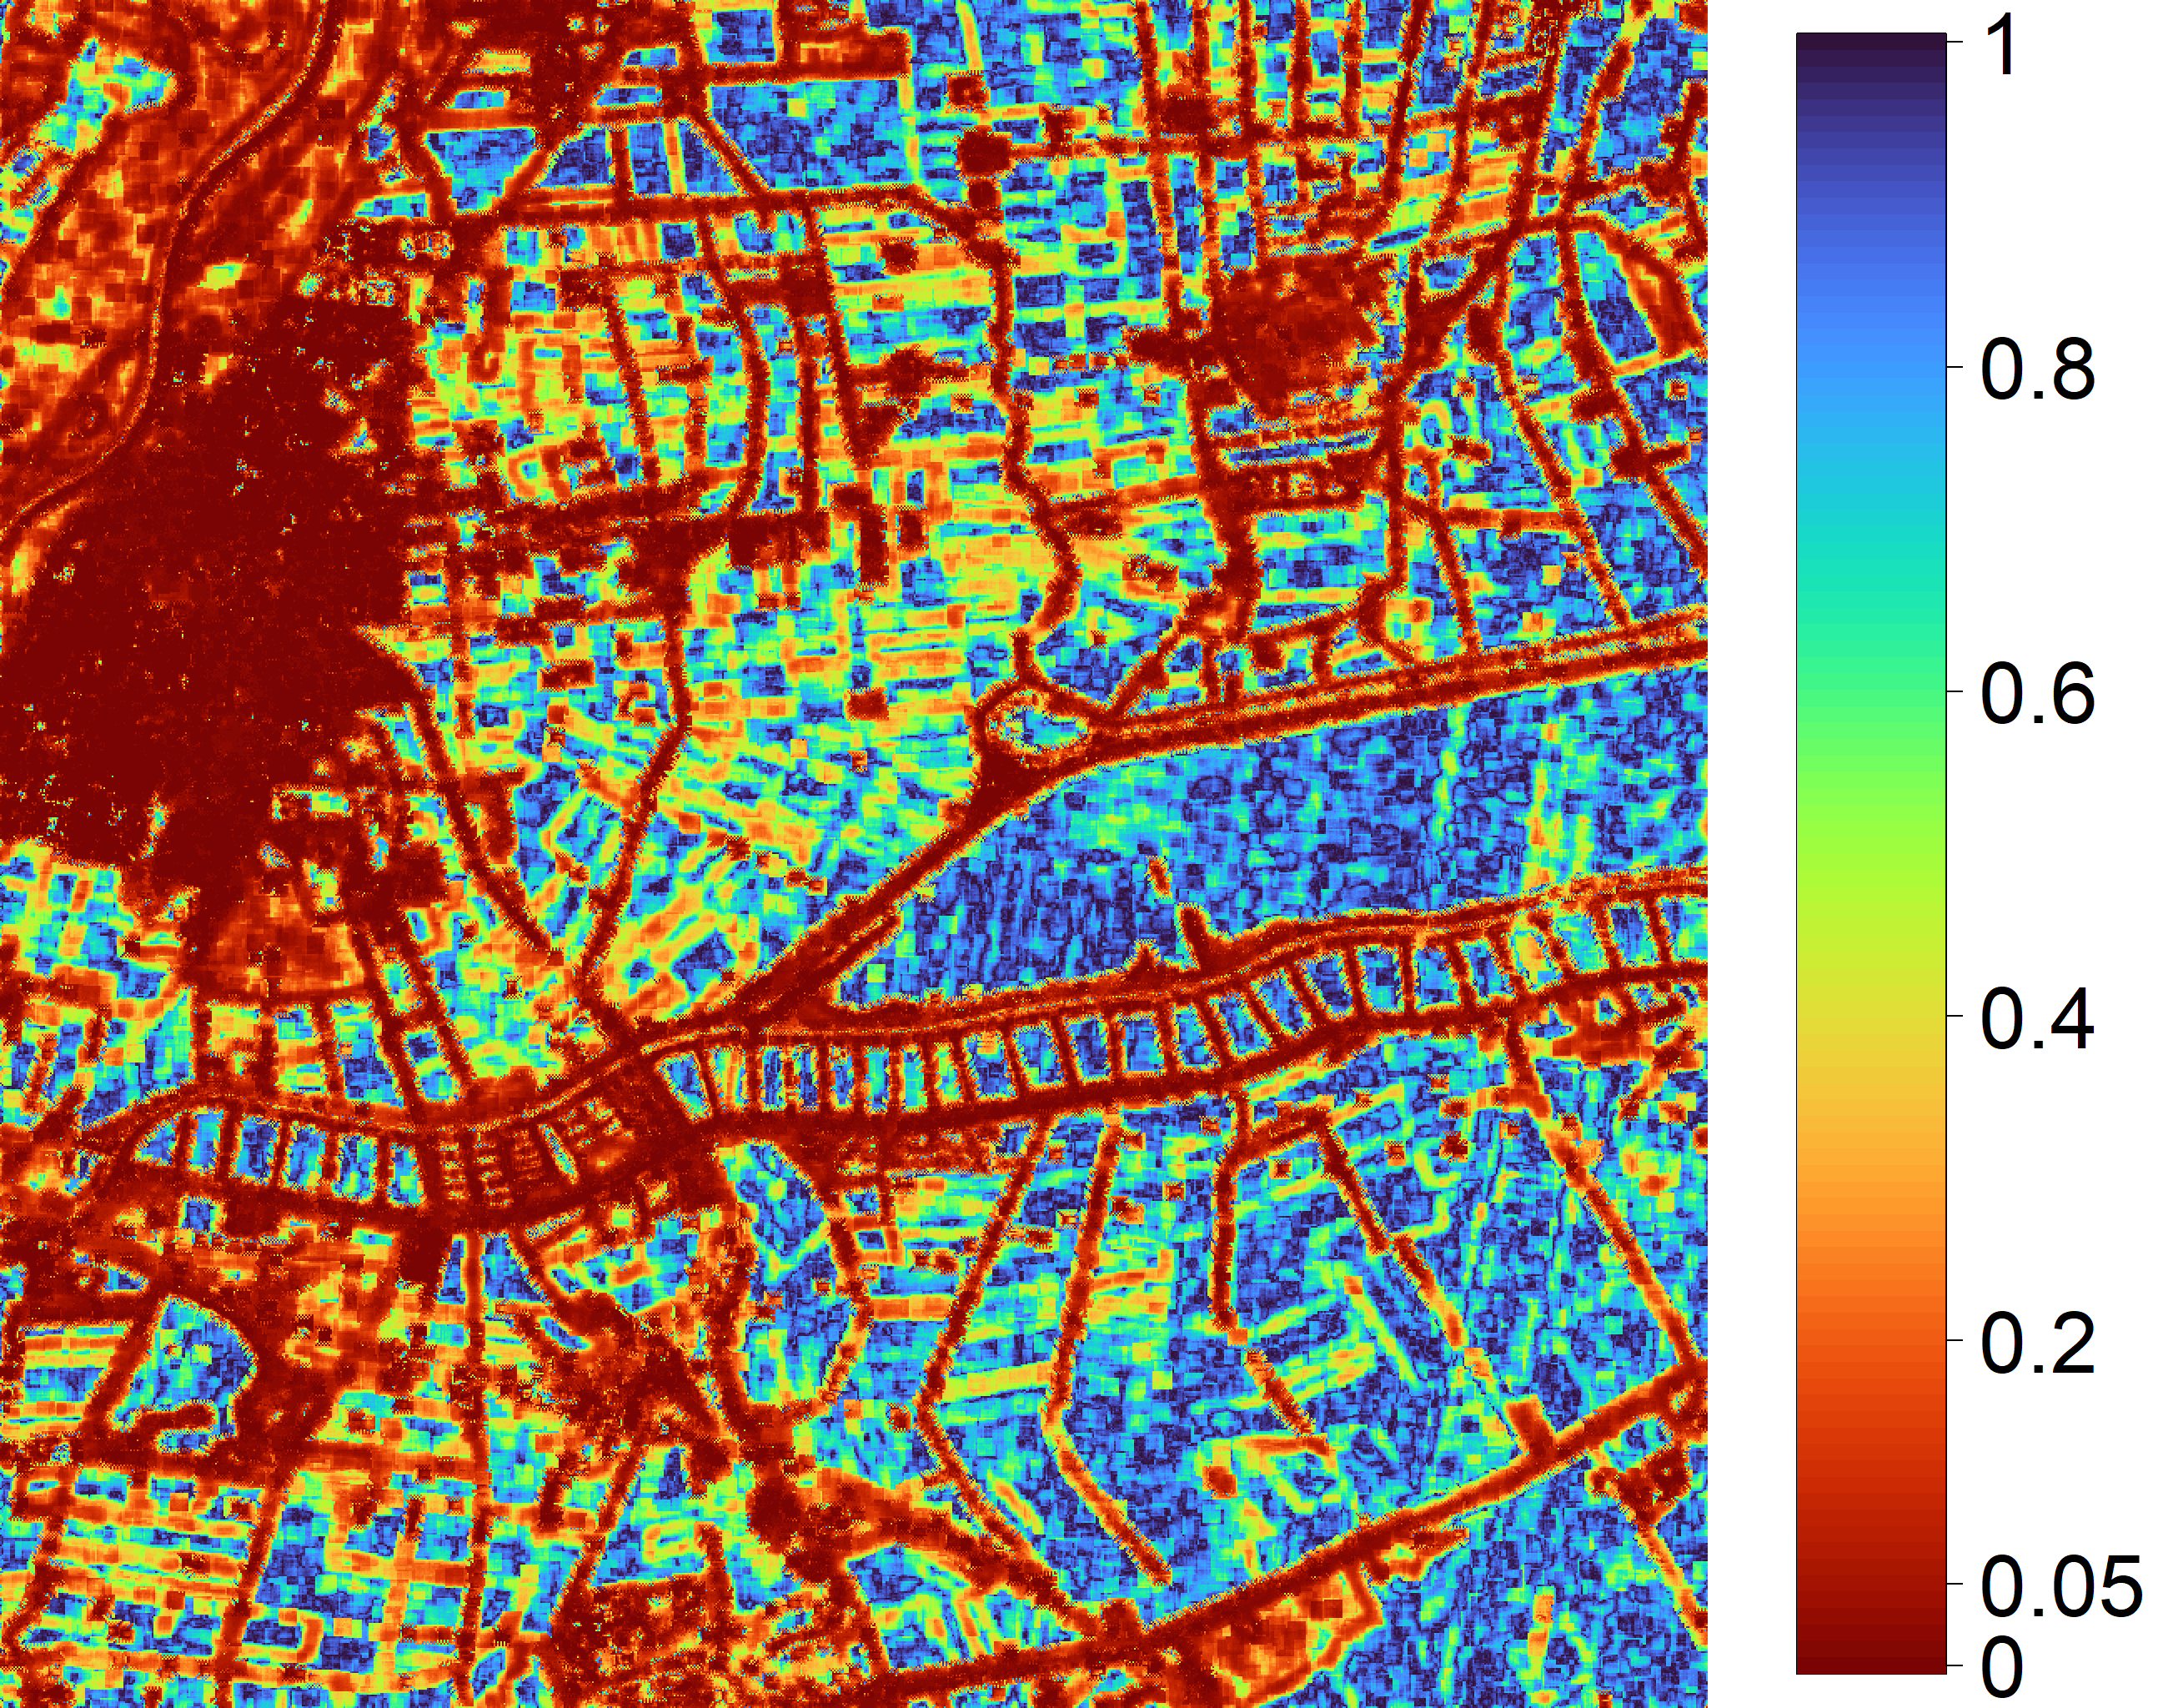
\includegraphics[width=\linewidth]{./Figures/p-values_munich1024_eta3.0_lambda085_5x11_b100.png}
\caption{$p$-value map ($\eta=3$)}
\label{fig:muc4}
\end{subfigure}\hfill
\begin{subfigure}[t]{0.19\textwidth}
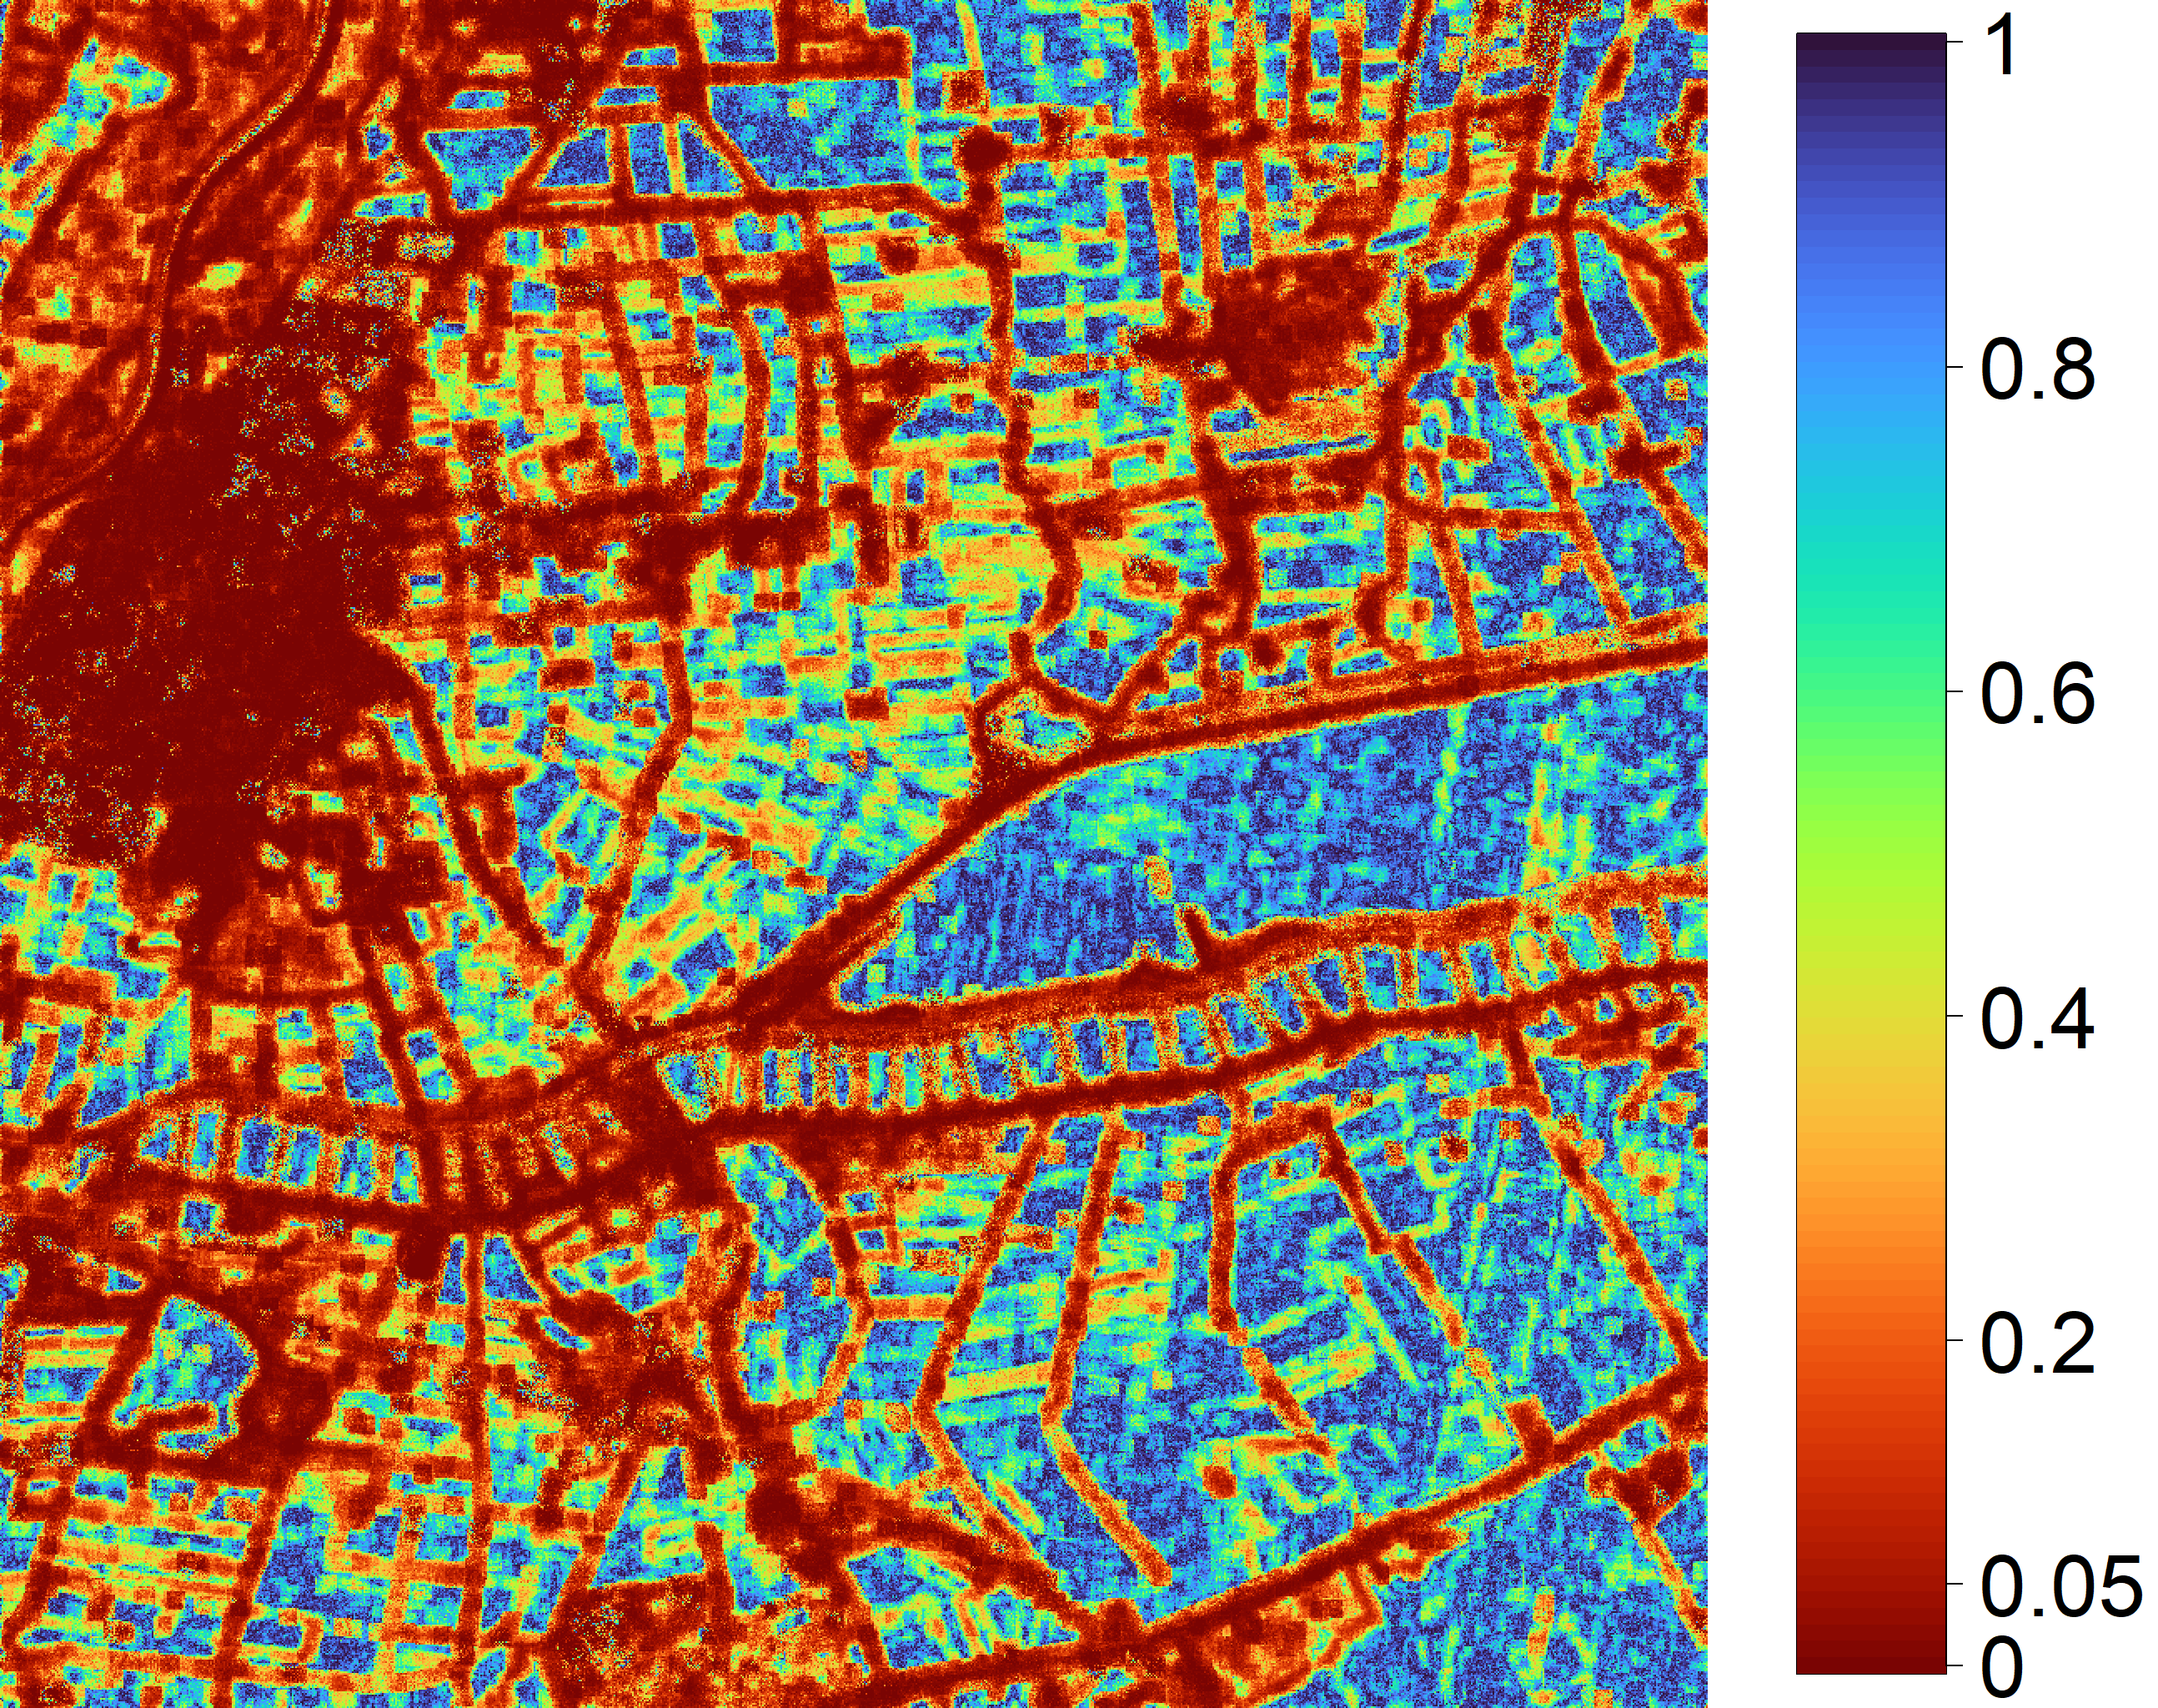
\includegraphics[width=\linewidth]{./Figures/p-values_munich1024_eta_4.png}
\caption{$p$-value map ($\eta=4$)}
\label{fig:muc5}
\end{subfigure}

\vspace{4pt}

\begin{subfigure}[t]{0.18\textwidth}
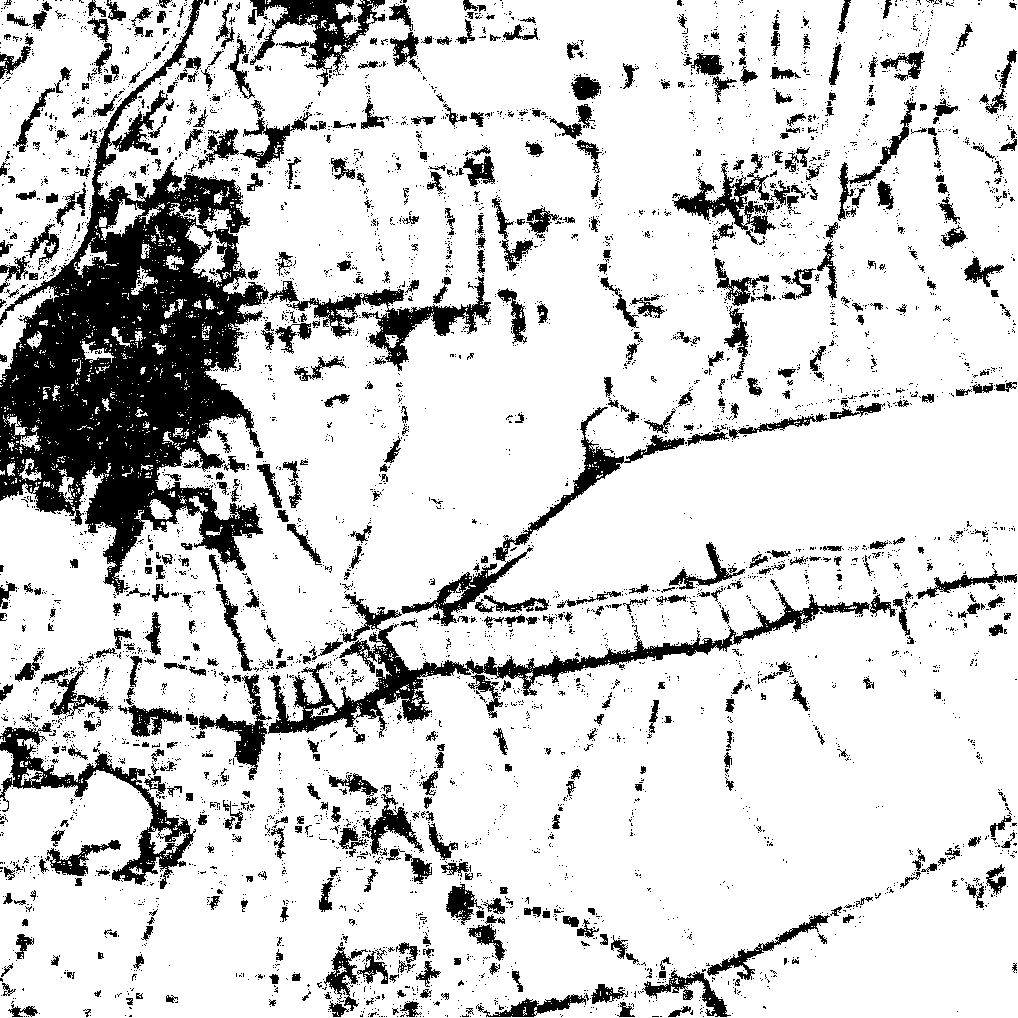
\includegraphics[width=\linewidth]{./Figures/H_005_munich1024_lambda085_7x7.png}
\caption{Binary map ($7\times7$)}
\label{fig:munc1}
\end{subfigure}\hfill
\begin{subfigure}[t]{0.18\textwidth}
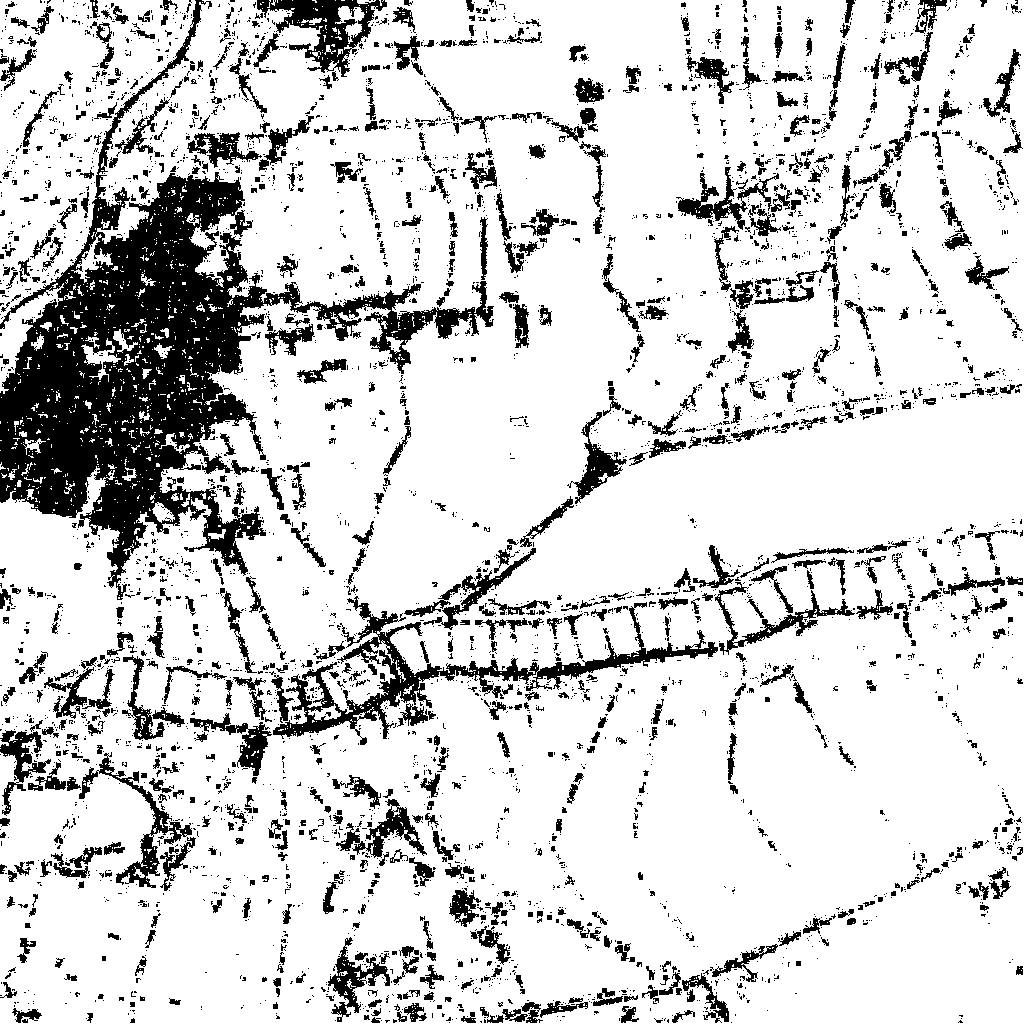
\includegraphics[width=\linewidth]{./Figures/H_005_munich1024_eta1.0_lambda085_5x11b100.png}
\caption{Binary map ($\eta=1$)}
\label{fig:munc2}
\end{subfigure}\hfill
\begin{subfigure}[t]{0.18\textwidth}
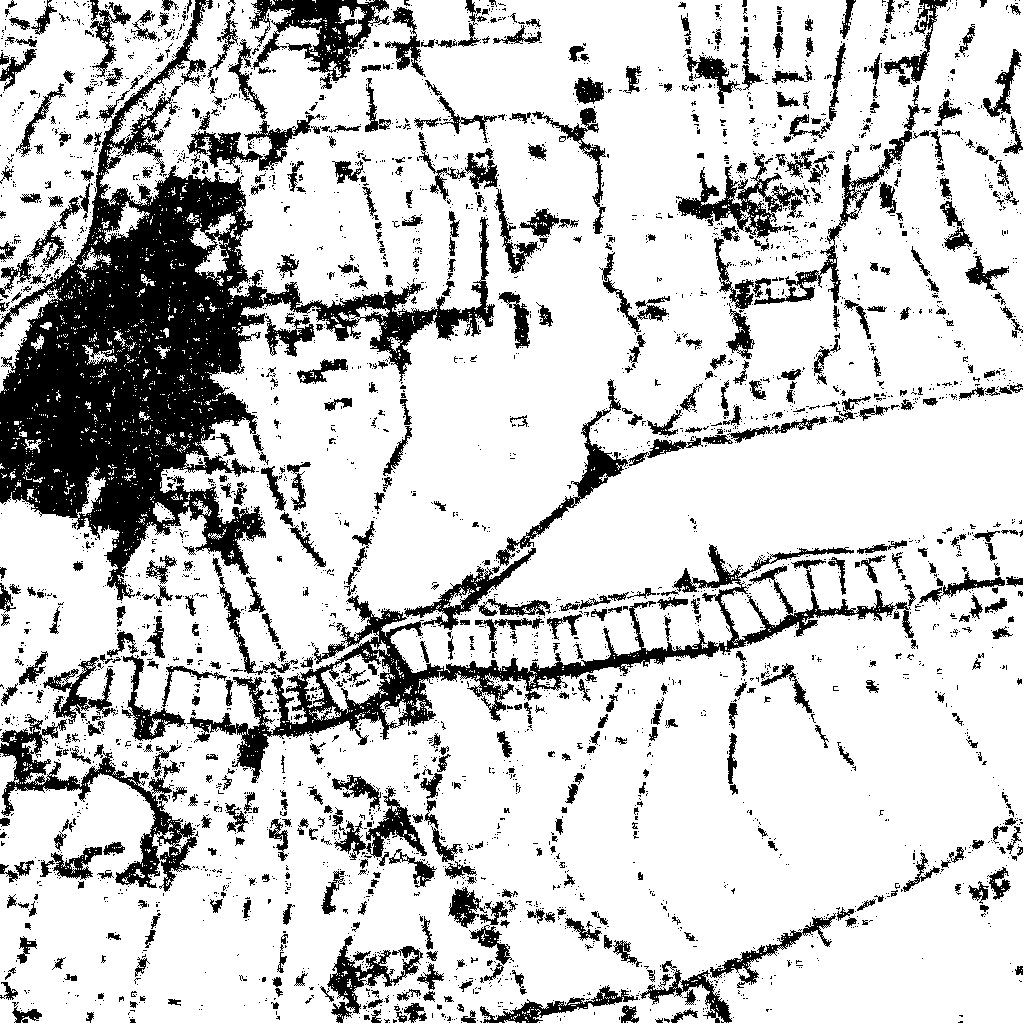
\includegraphics[width=\linewidth]{./Figures/H_005_munich1024_eta2.0_lambda085_5x11b100.png}
\caption{Binary map ($\eta=2$)}
\label{fig:munc3}
\end{subfigure}\hfill
\begin{subfigure}[t]{0.18\textwidth}
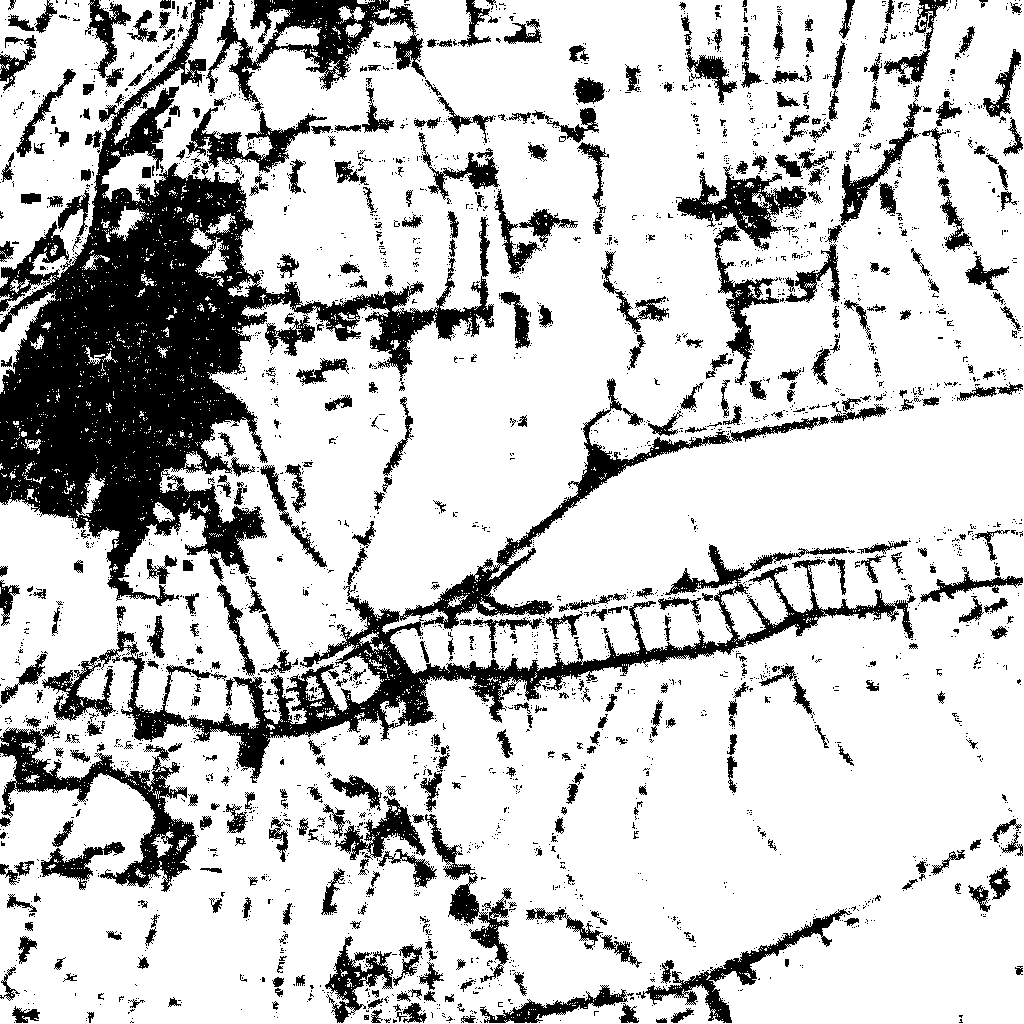
\includegraphics[width=\linewidth]{./Figures/H_005_munich1024_eta3.0_lambda085_5x11b100.png}
\caption{Binary map ($\eta=3$)}
\label{fig:munc4}
\end{subfigure}\hfill
\begin{subfigure}[t]{0.18\textwidth}
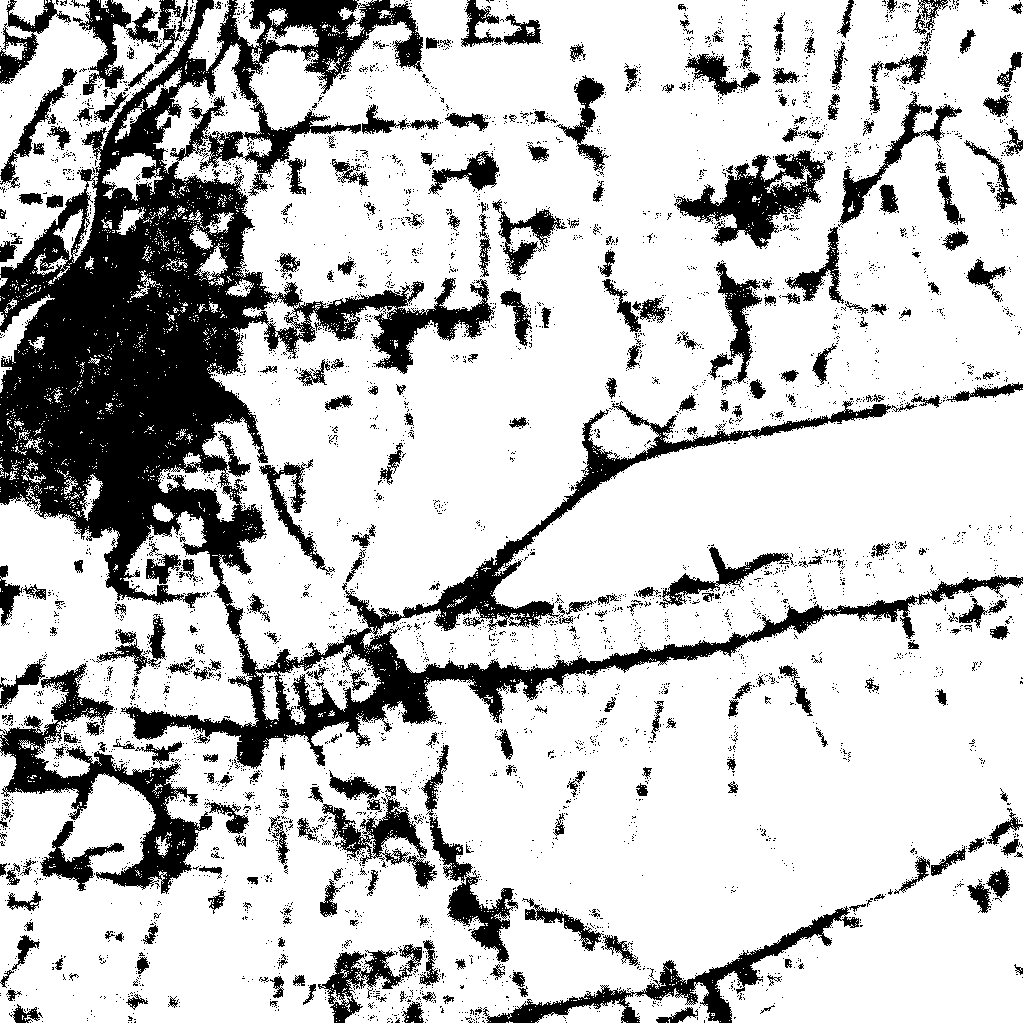
\includegraphics[width=\linewidth]{./Figures/H_005_munich_eta_4.png}
\caption{Binary map ($\eta=4$)}
\label{fig:munc5}
\end{subfigure}

\caption{Detection of heterogeneous areas in a SAR image over the outskirts of Munich. (a) $p$-value map with a fixed $7\times7$ window. (b–e) $p$-value maps with adaptive windows ($W_{\min}=5$, $W_{\max}=11$) for $\eta=1$--$4$. (f–j) Binary decision maps at $0.05$ significance level.}
\label{fig:munich}
\end{figure*}

\begin{figure*}[!t]
\centering
\captionsetup{font=footnotesize}
\captionsetup[sub]{aboveskip=2pt,belowskip=2pt}

\begin{subfigure}[t]{0.19\textwidth}
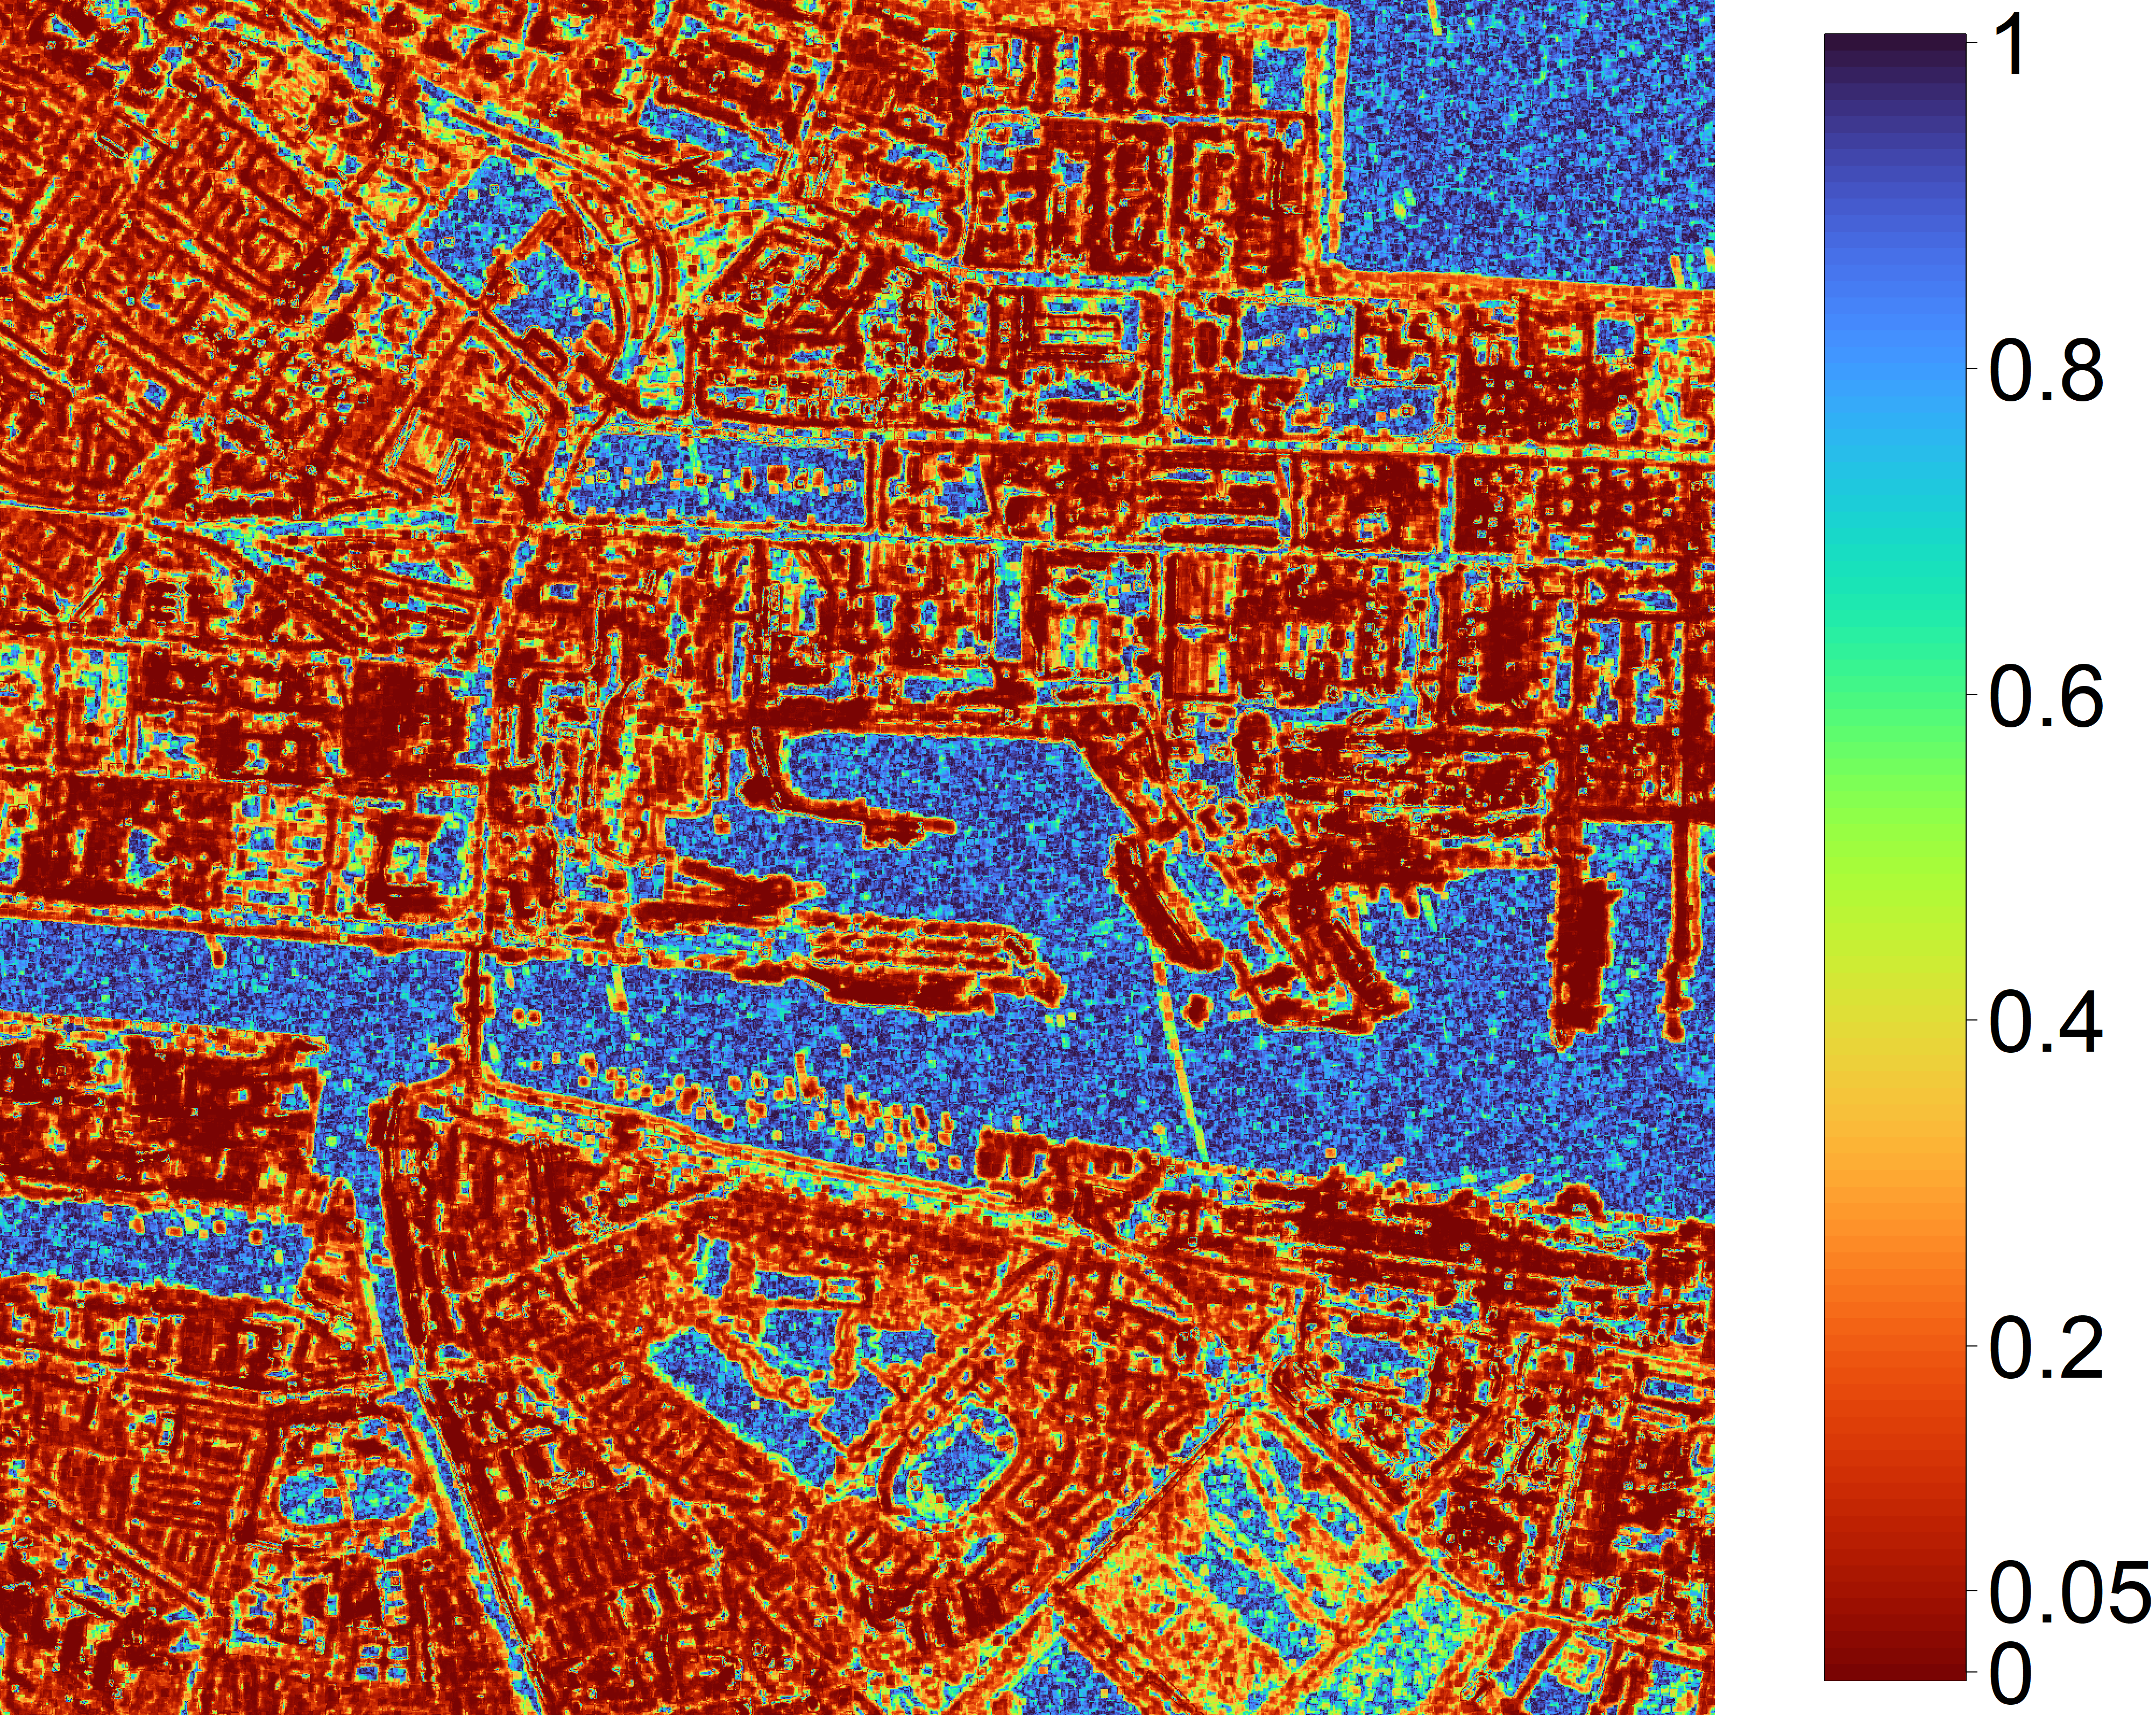
\includegraphics[width=\linewidth]{./Figures/p-values_dublinlambda085_7x7_b100.png}
\caption{$p$-value map ($7\times7$)}
\label{fig:duc1}
\end{subfigure}\hfill
\begin{subfigure}[t]{0.19\textwidth}
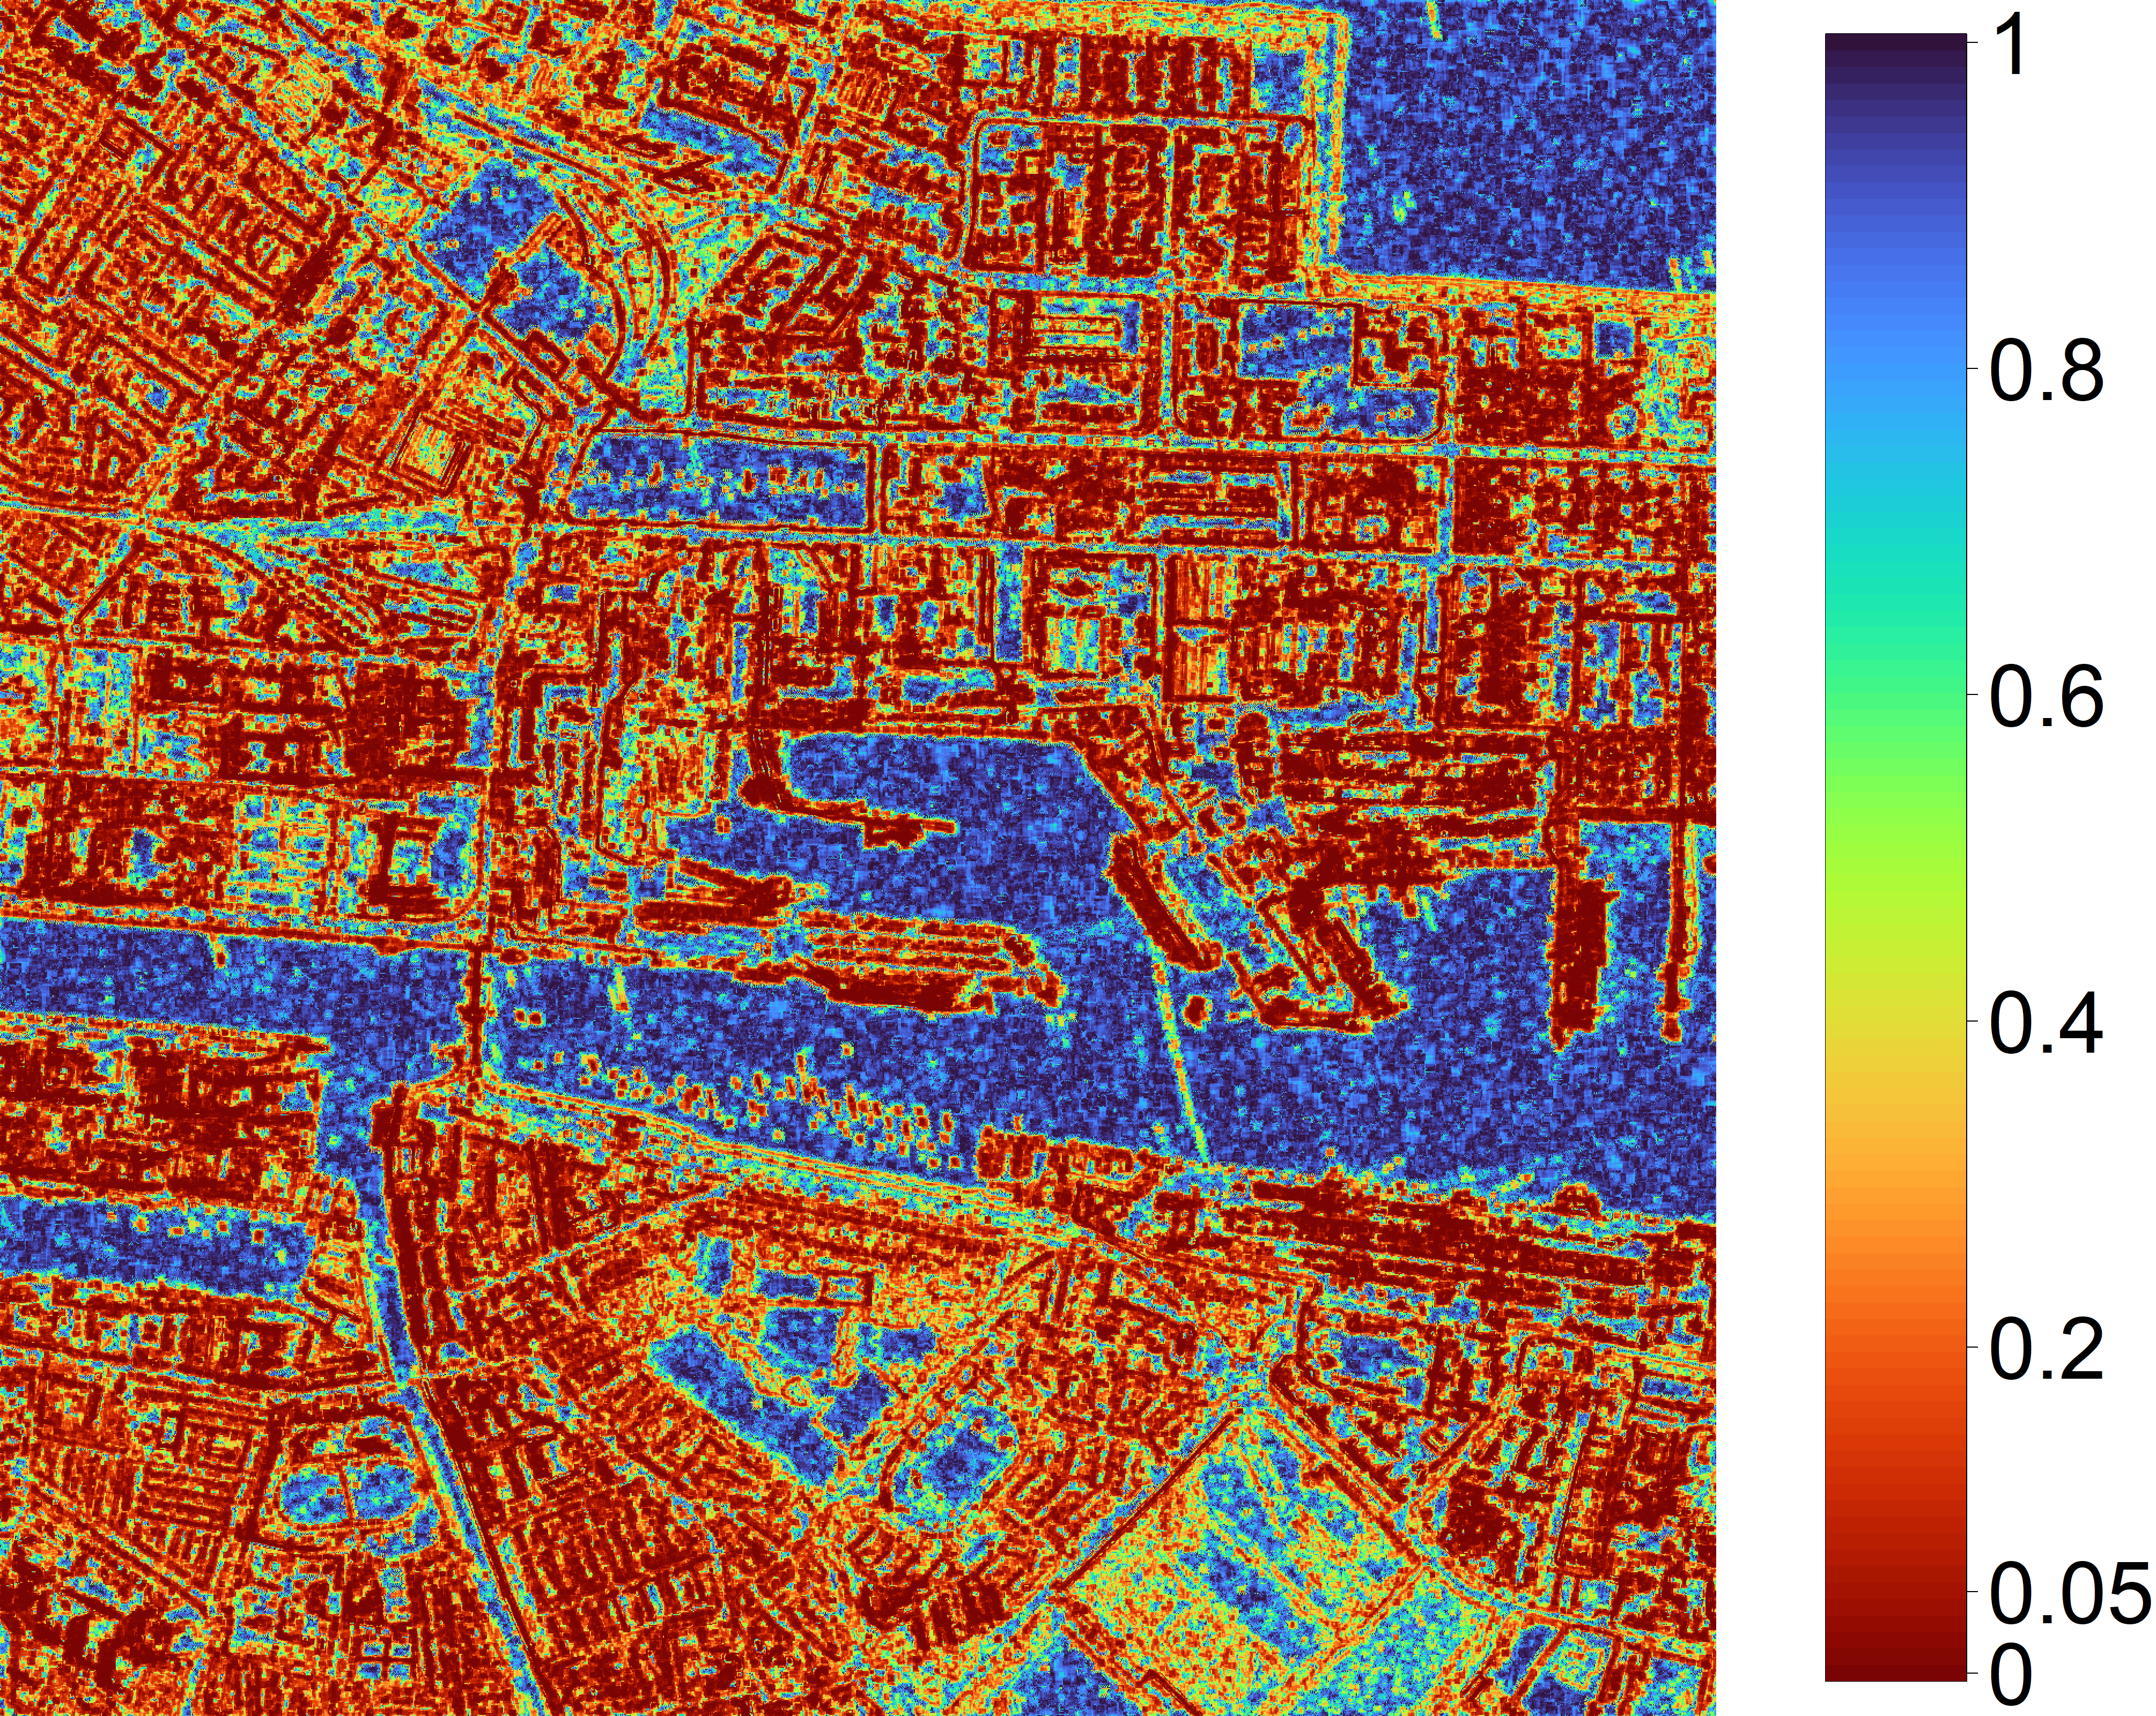
\includegraphics[width=\linewidth]{./Figures/p-values_dublin1600_eta1.0nn_lambda085_5x11_b100.png}
\caption{$p$-value map ($\eta=1$)}
\label{fig:duc2}
\end{subfigure}\hfill
\begin{subfigure}[t]{0.19\textwidth}
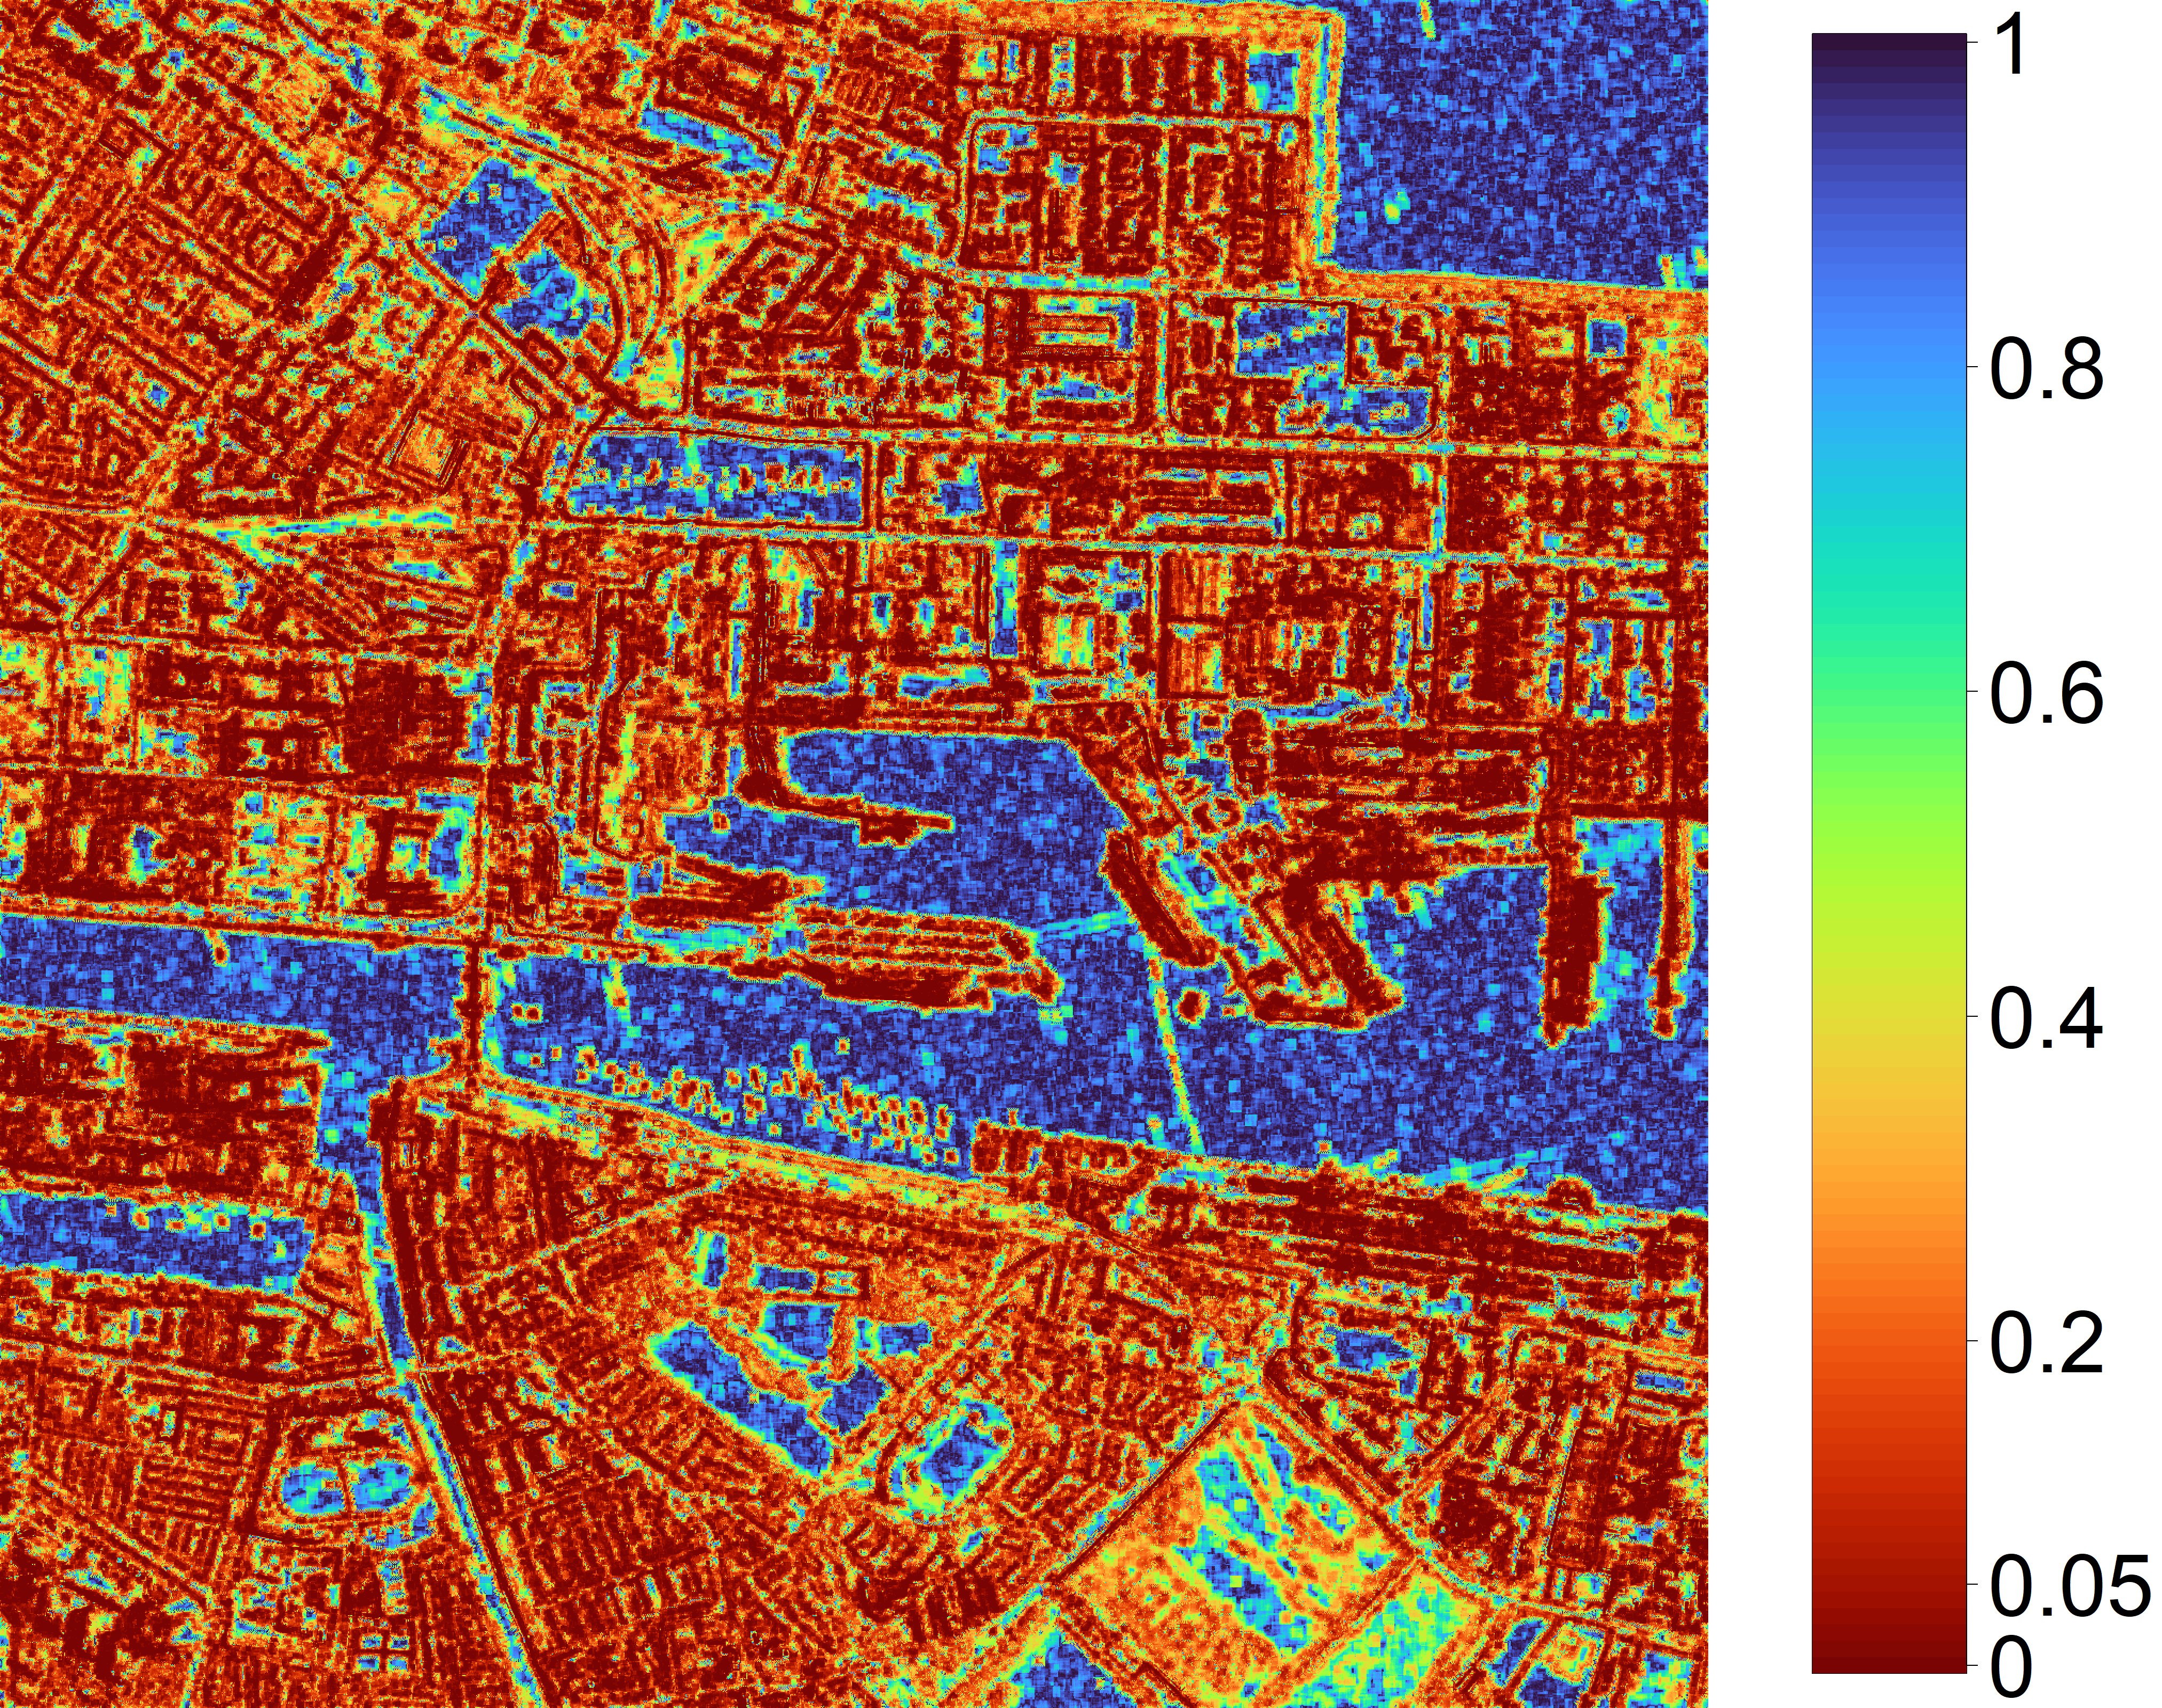
\includegraphics[width=\linewidth]{./Figures/p-values_dublin1600_eta2.0_lambda085_5x11_b1005.png}
\caption{$p$-value map ($\eta=2$)}
\label{fig:duc3}
\end{subfigure}\hfill
\begin{subfigure}[t]{0.19\textwidth}
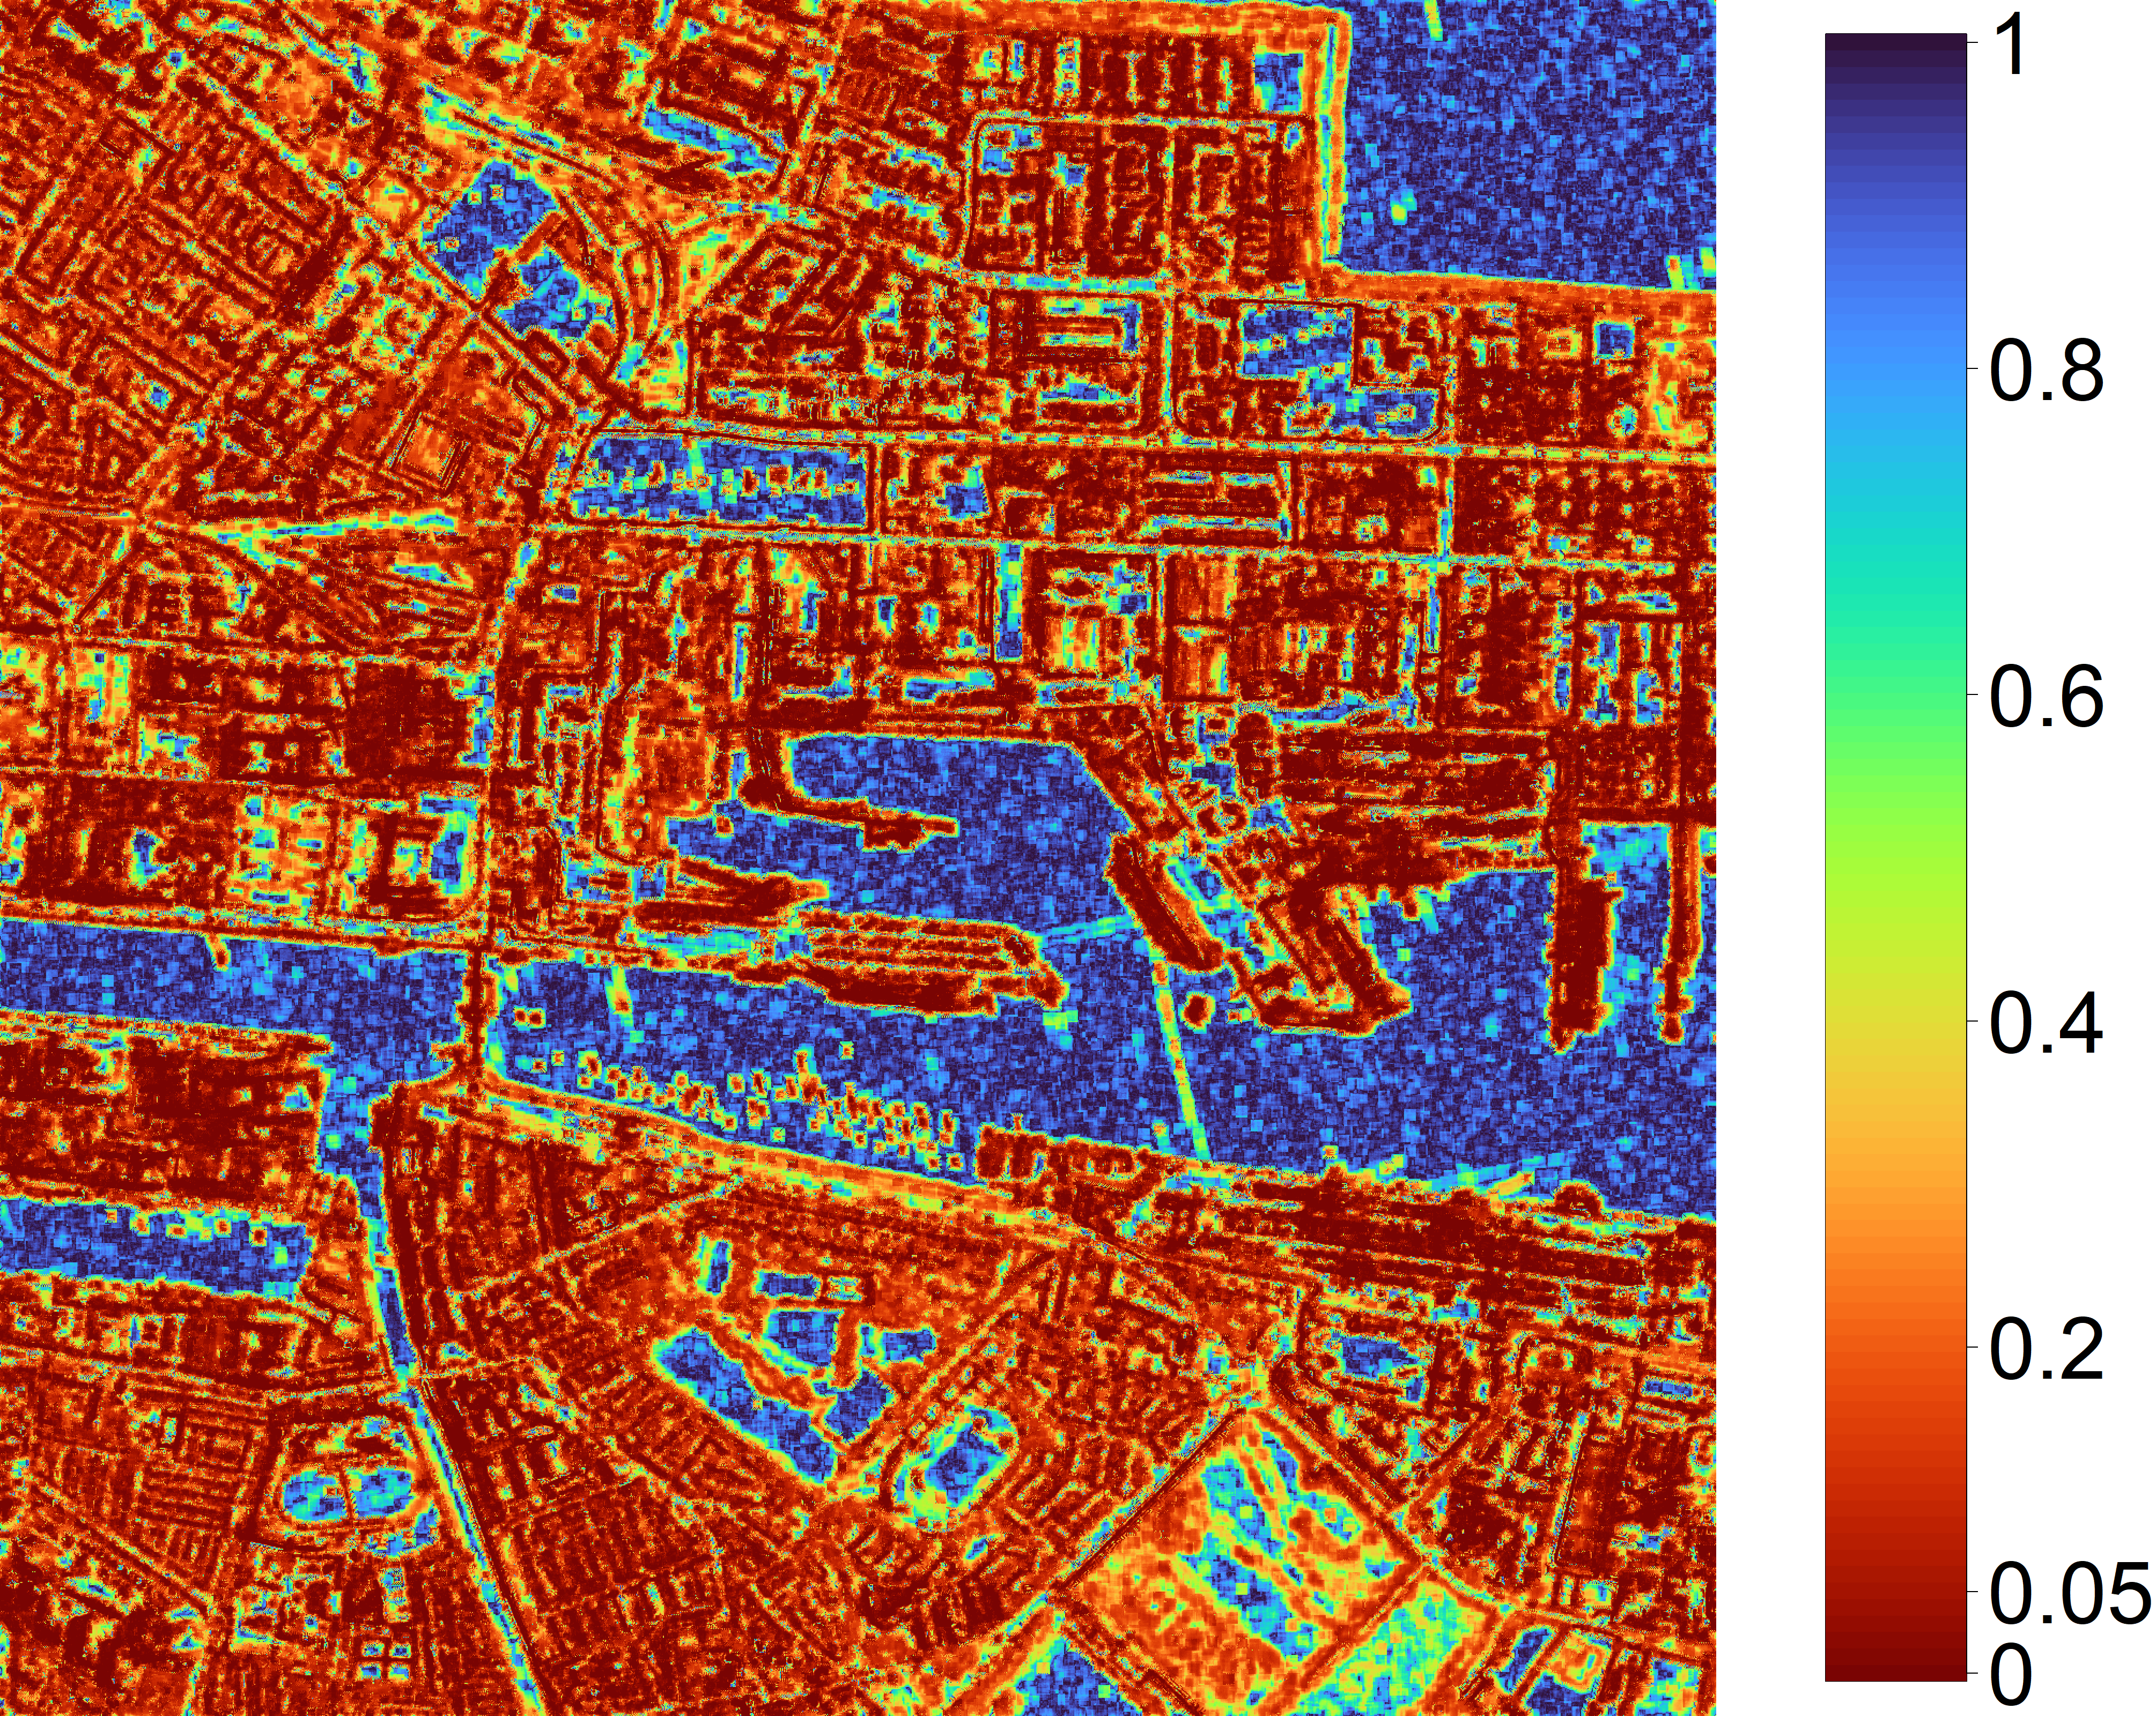
\includegraphics[width=\linewidth]{./Figures/p-values_dublin1600_eta3.0_lambda085_5x11_b100.png}
\caption{$p$-value map ($\eta=3$)}
\label{fig:duc4}
\end{subfigure}\hfill
\begin{subfigure}[t]{0.19\textwidth}
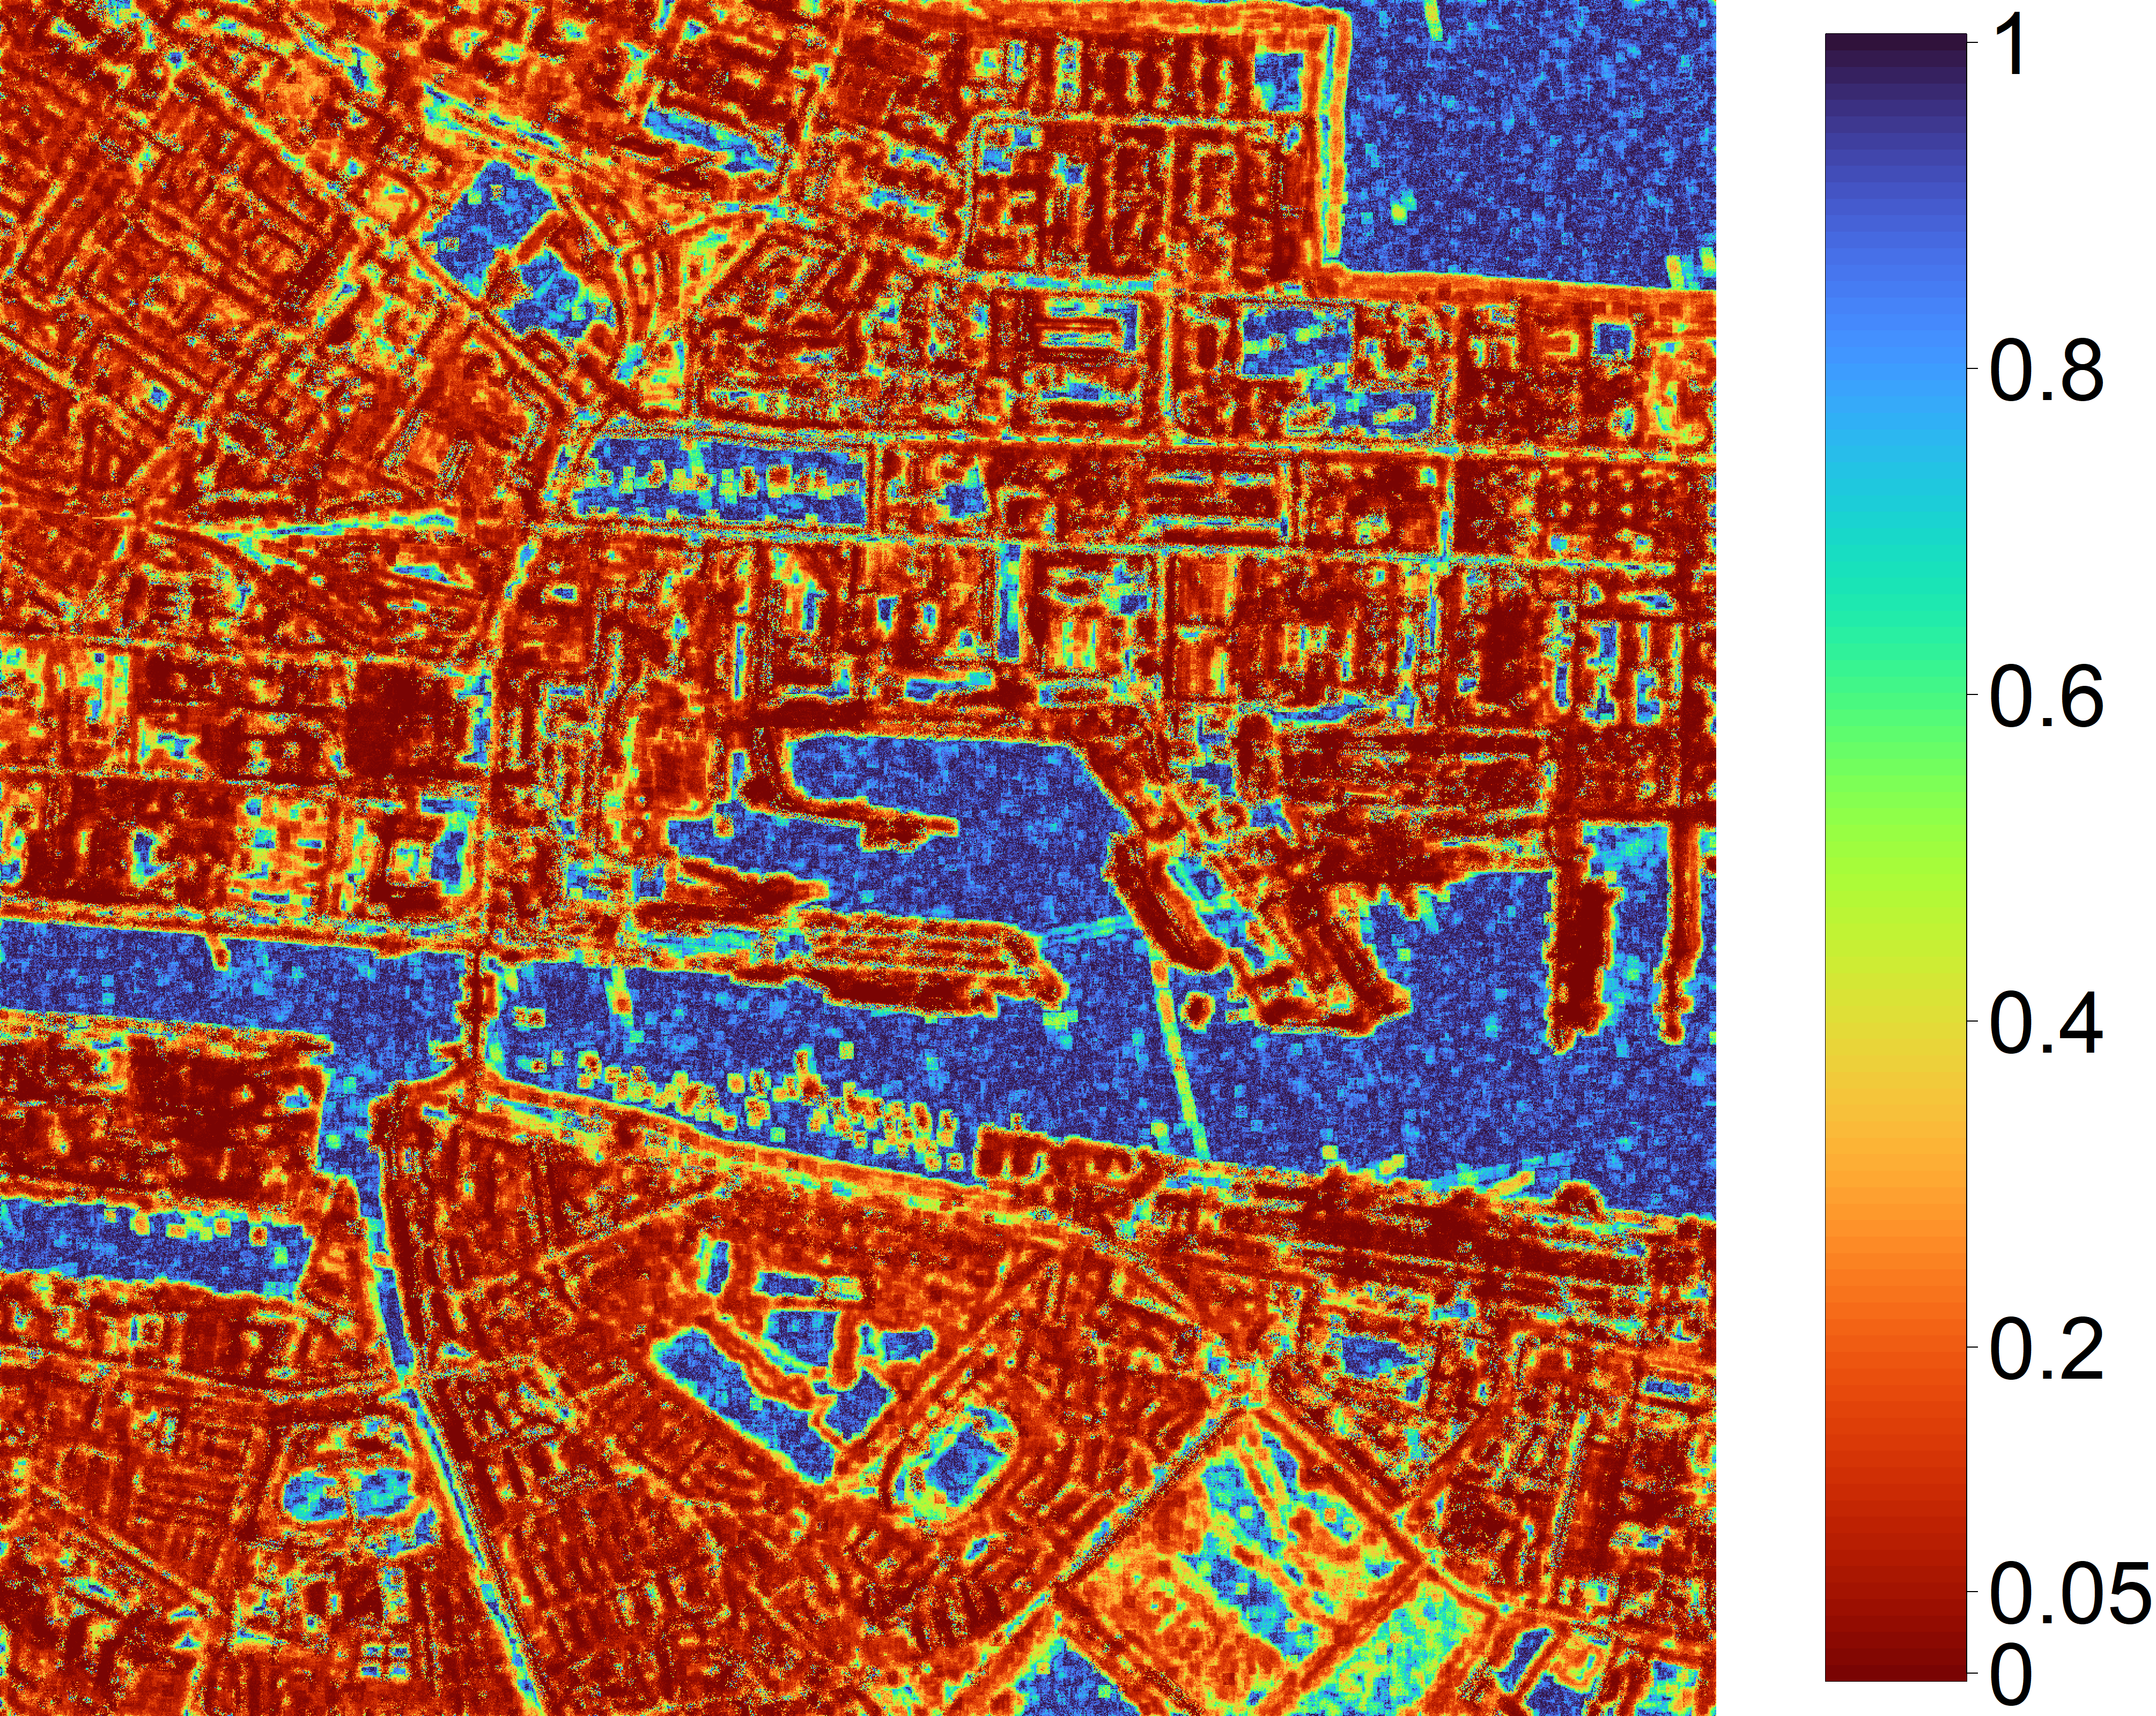
\includegraphics[width=\linewidth]{./Figures/p-values_dublin_eta4.png}
\caption{$p$-value map ($\eta=4$)}
\label{fig:duc5}
\end{subfigure}

\vspace{4pt}

\begin{subfigure}[t]{0.18\textwidth}
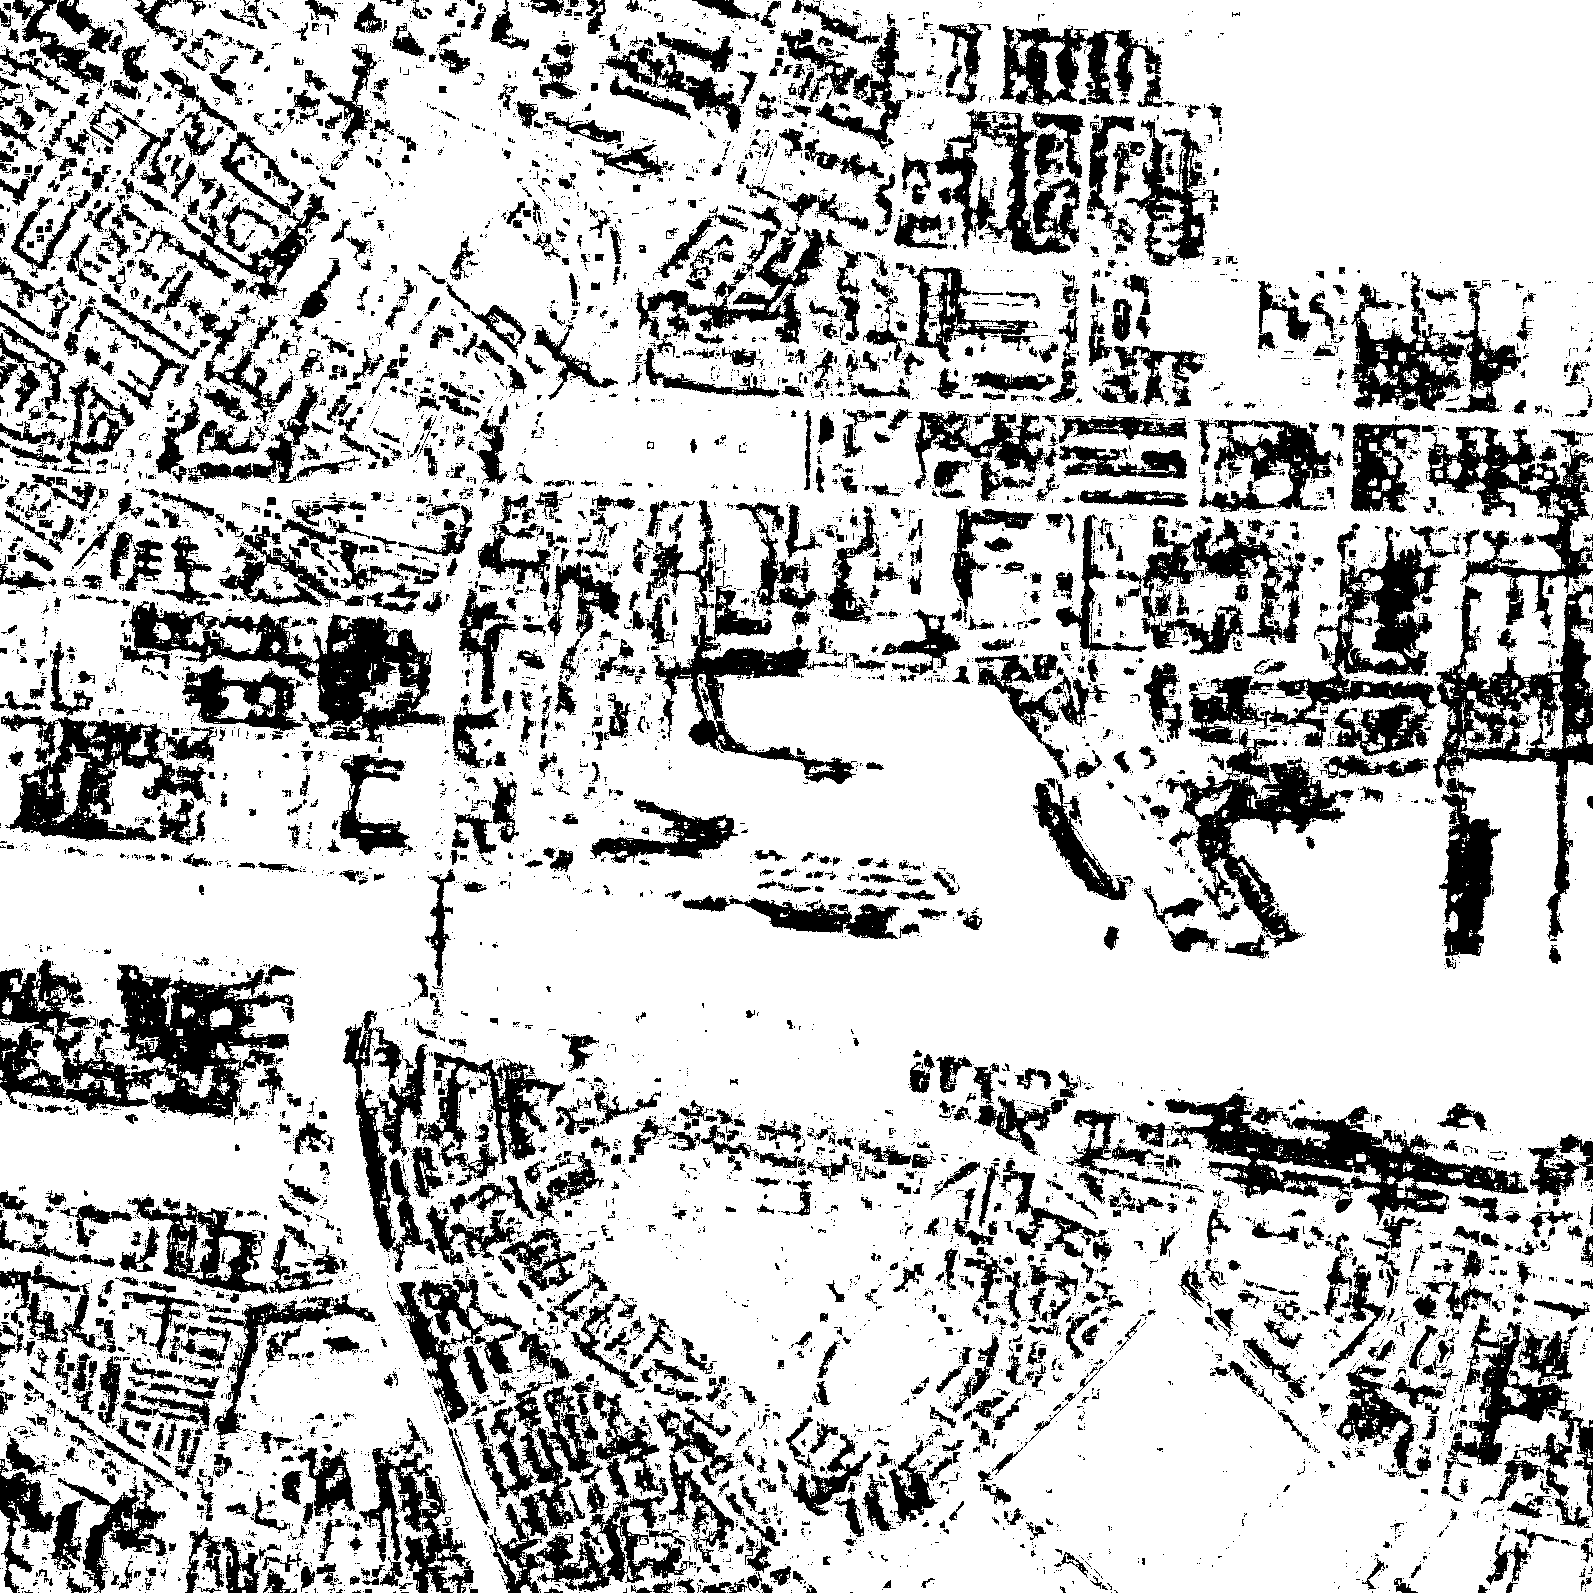
\includegraphics[width=\linewidth]{./Figures/H_005_dublin7x7_B100_lambda_081.png}
\caption{Binary map ($7\times7$)}
\label{fig:dubc1}
\end{subfigure}\hfill
\begin{subfigure}[t]{0.18\textwidth}
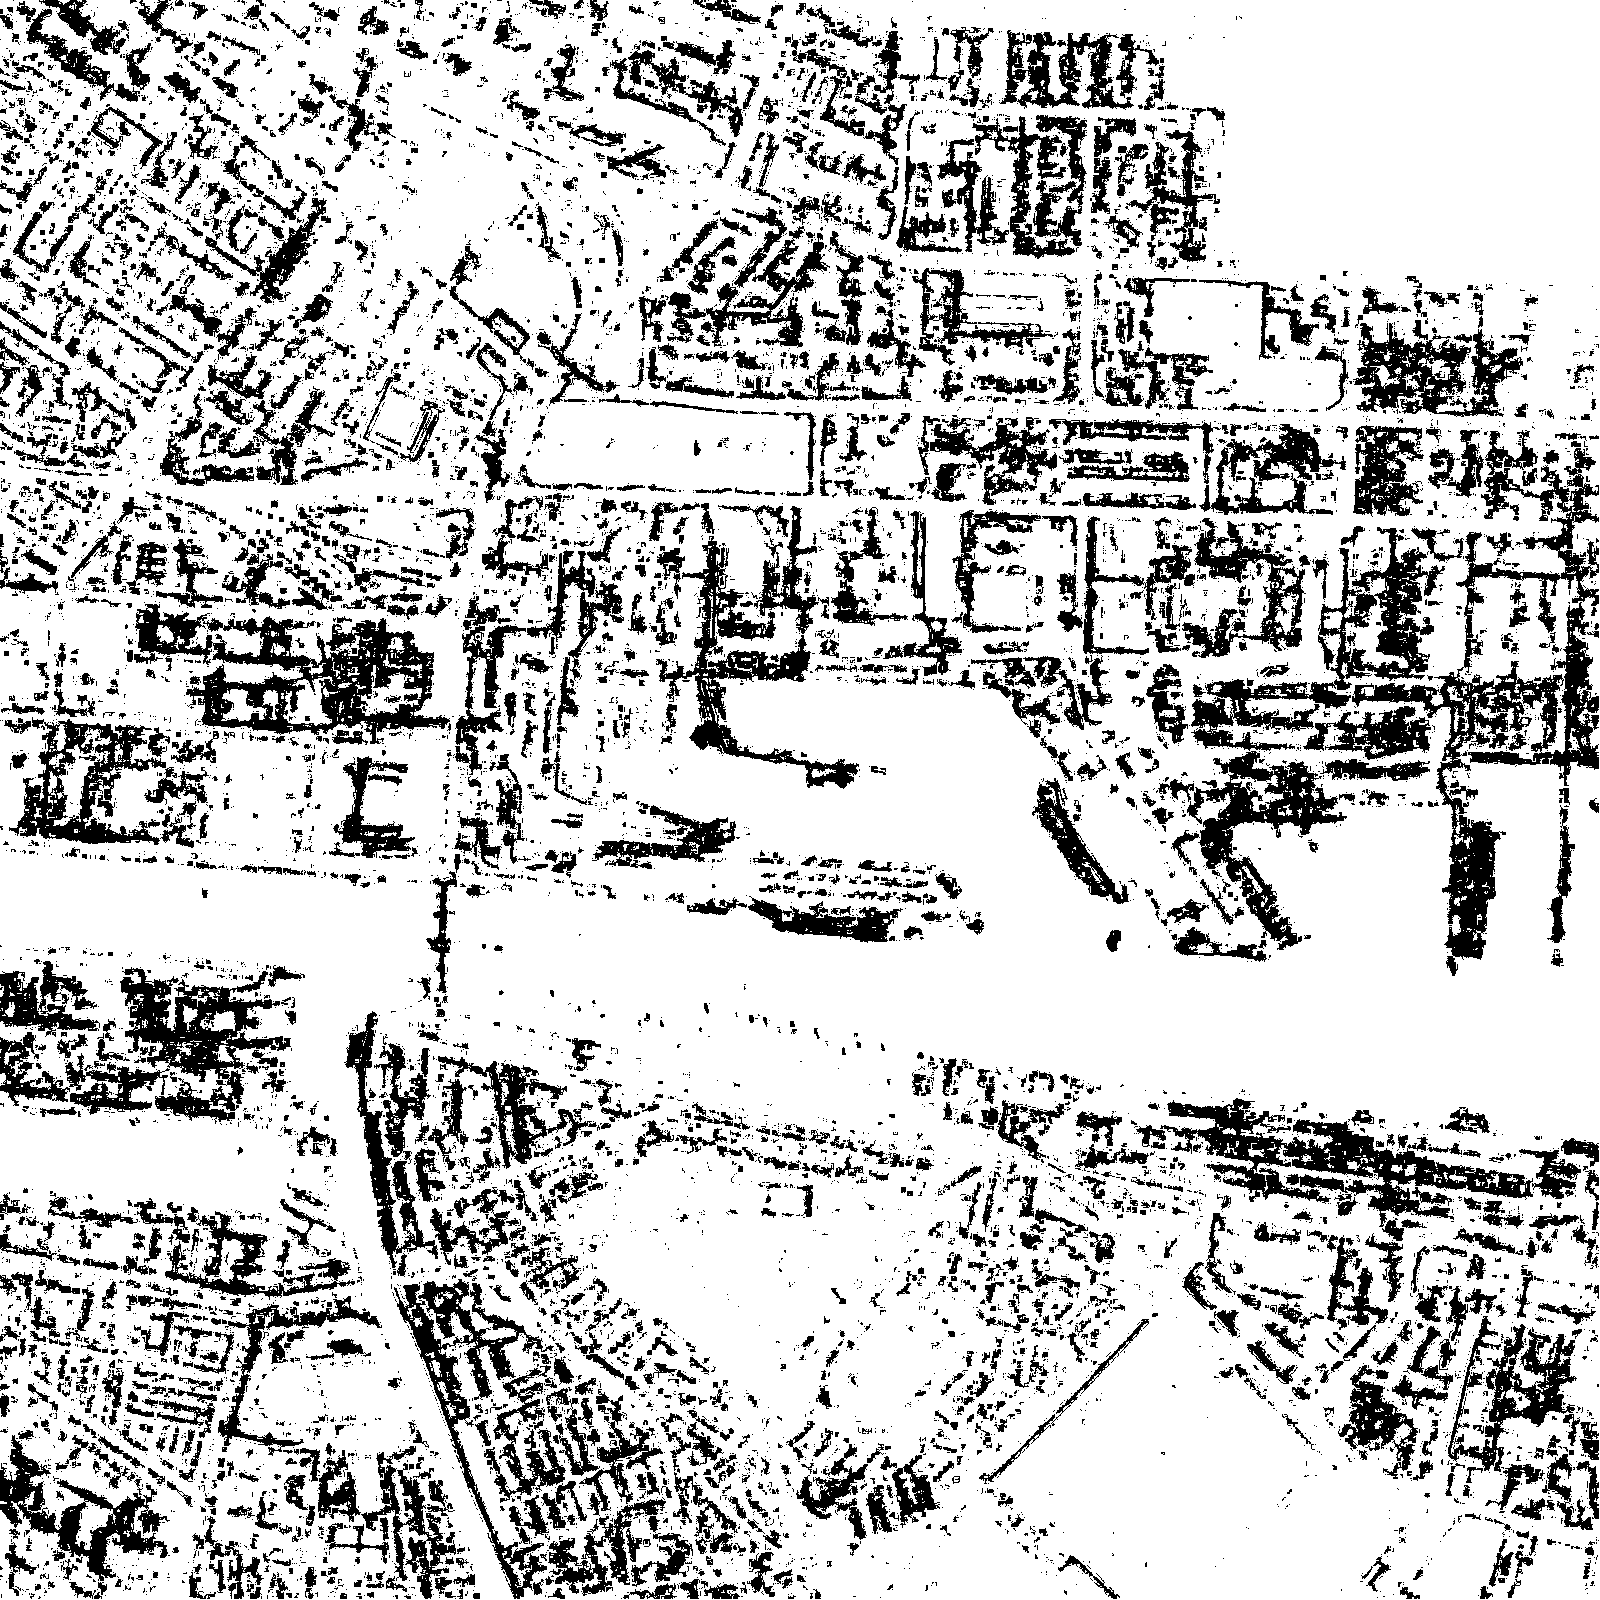
\includegraphics[width=\linewidth]{./Figures/H_005_dublin1600_eta1.0_lambda085_5x11_b100.png}
\caption{Binary map ($\eta=1$)}
\label{fig:dubc2}
\end{subfigure}\hfill
\begin{subfigure}[t]{0.18\textwidth}
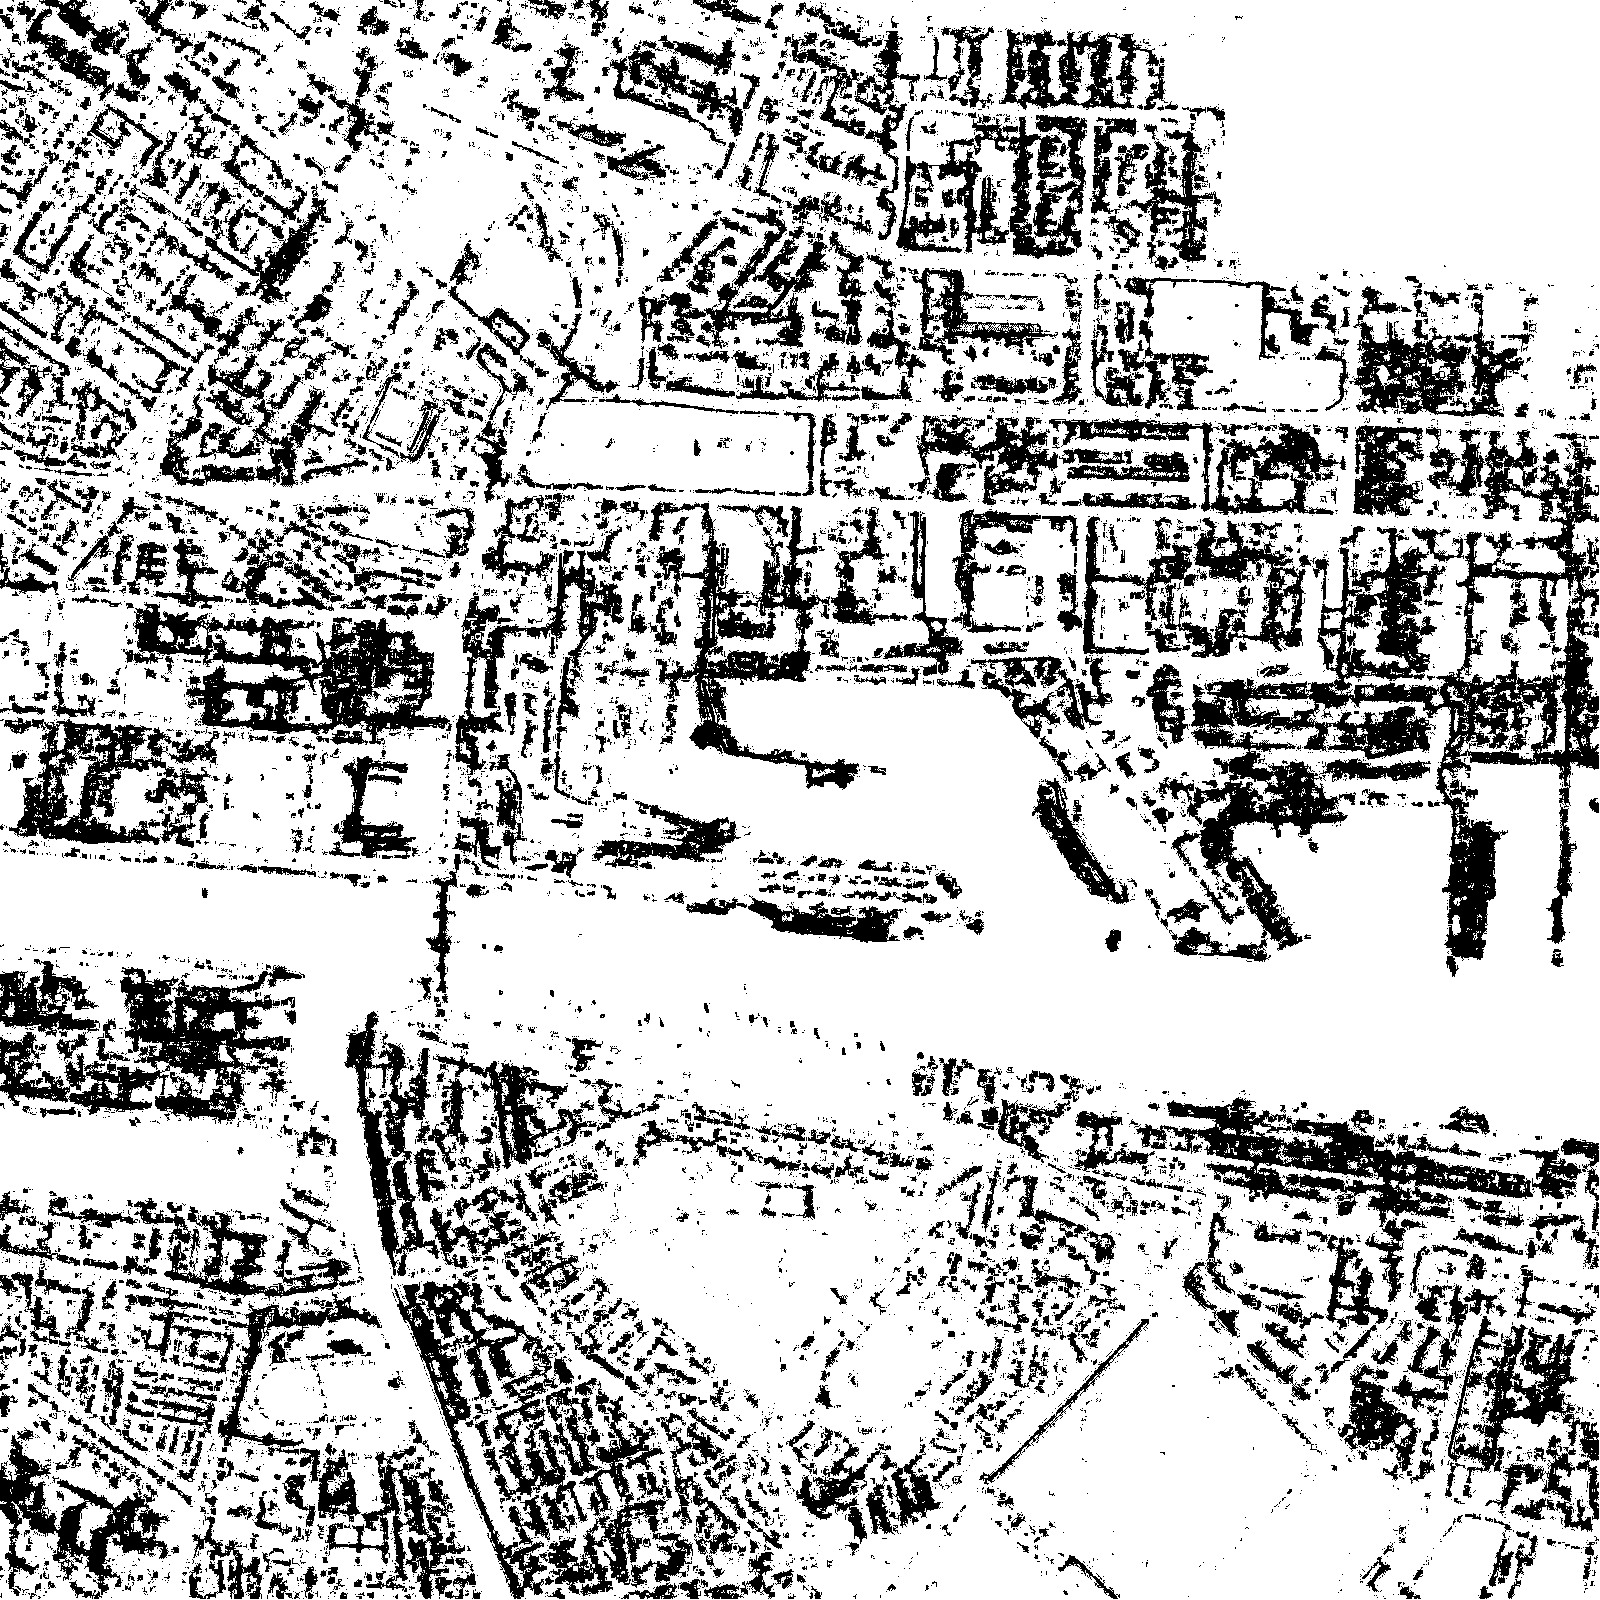
\includegraphics[width=\linewidth]{./Figures/H_005_dublin1600_eta2.0_lambda085_5x11_b1005.png}
\caption{Binary map ($\eta=2$)}
\label{fig:dubc3}
\end{subfigure}\hfill
\begin{subfigure}[t]{0.18\textwidth}
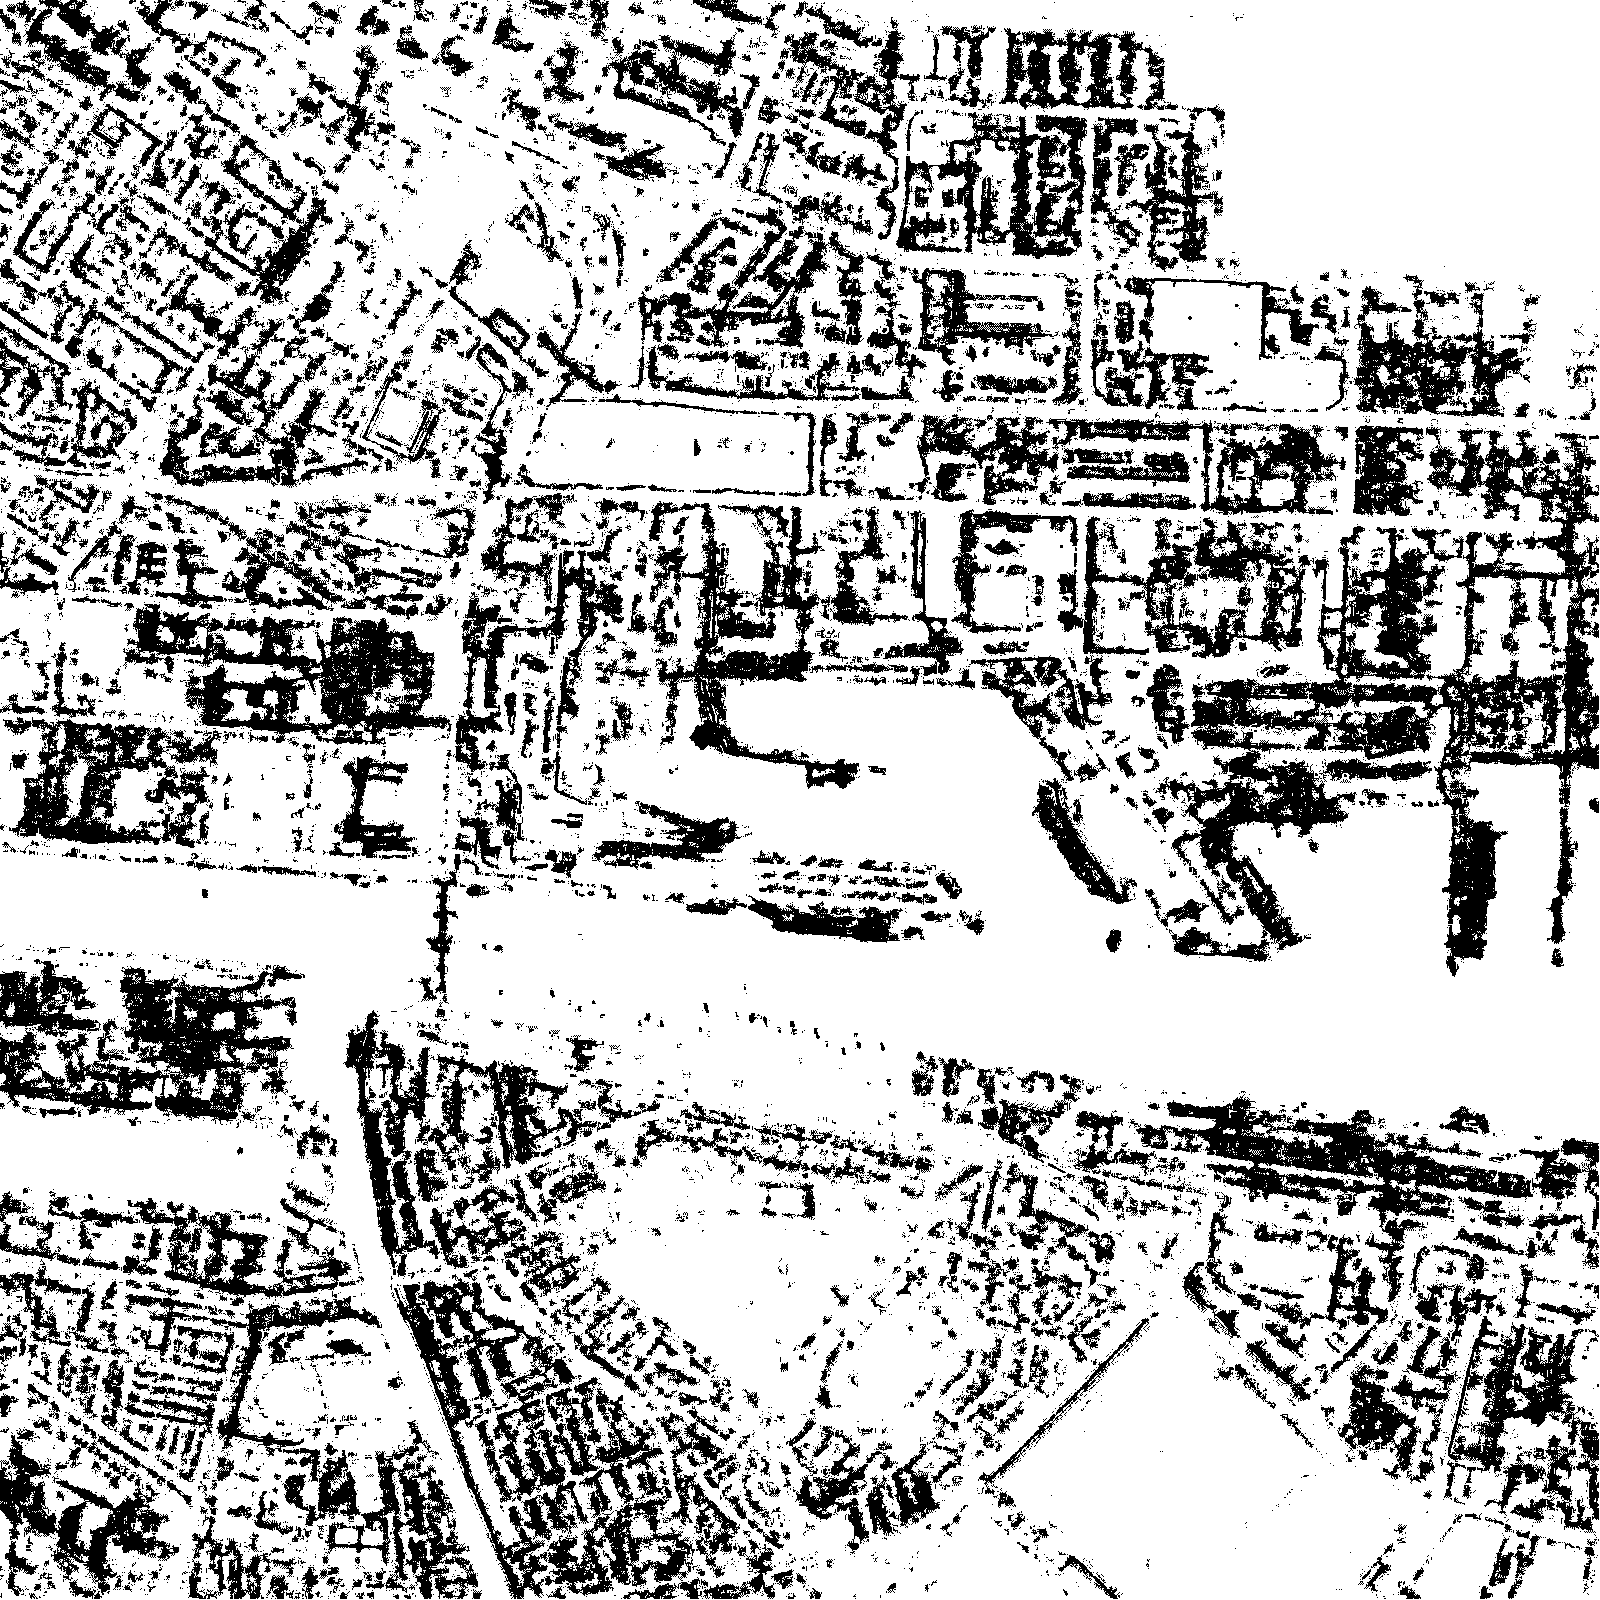
\includegraphics[width=\linewidth]{./Figures/H_005_dublin1600_OR_eta3.0_lambda085_5x11_b100.png}
\caption{Binary map ($\eta=3$)}
\label{fig:dubc4}
\end{subfigure}\hfill
\begin{subfigure}[t]{0.18\textwidth}
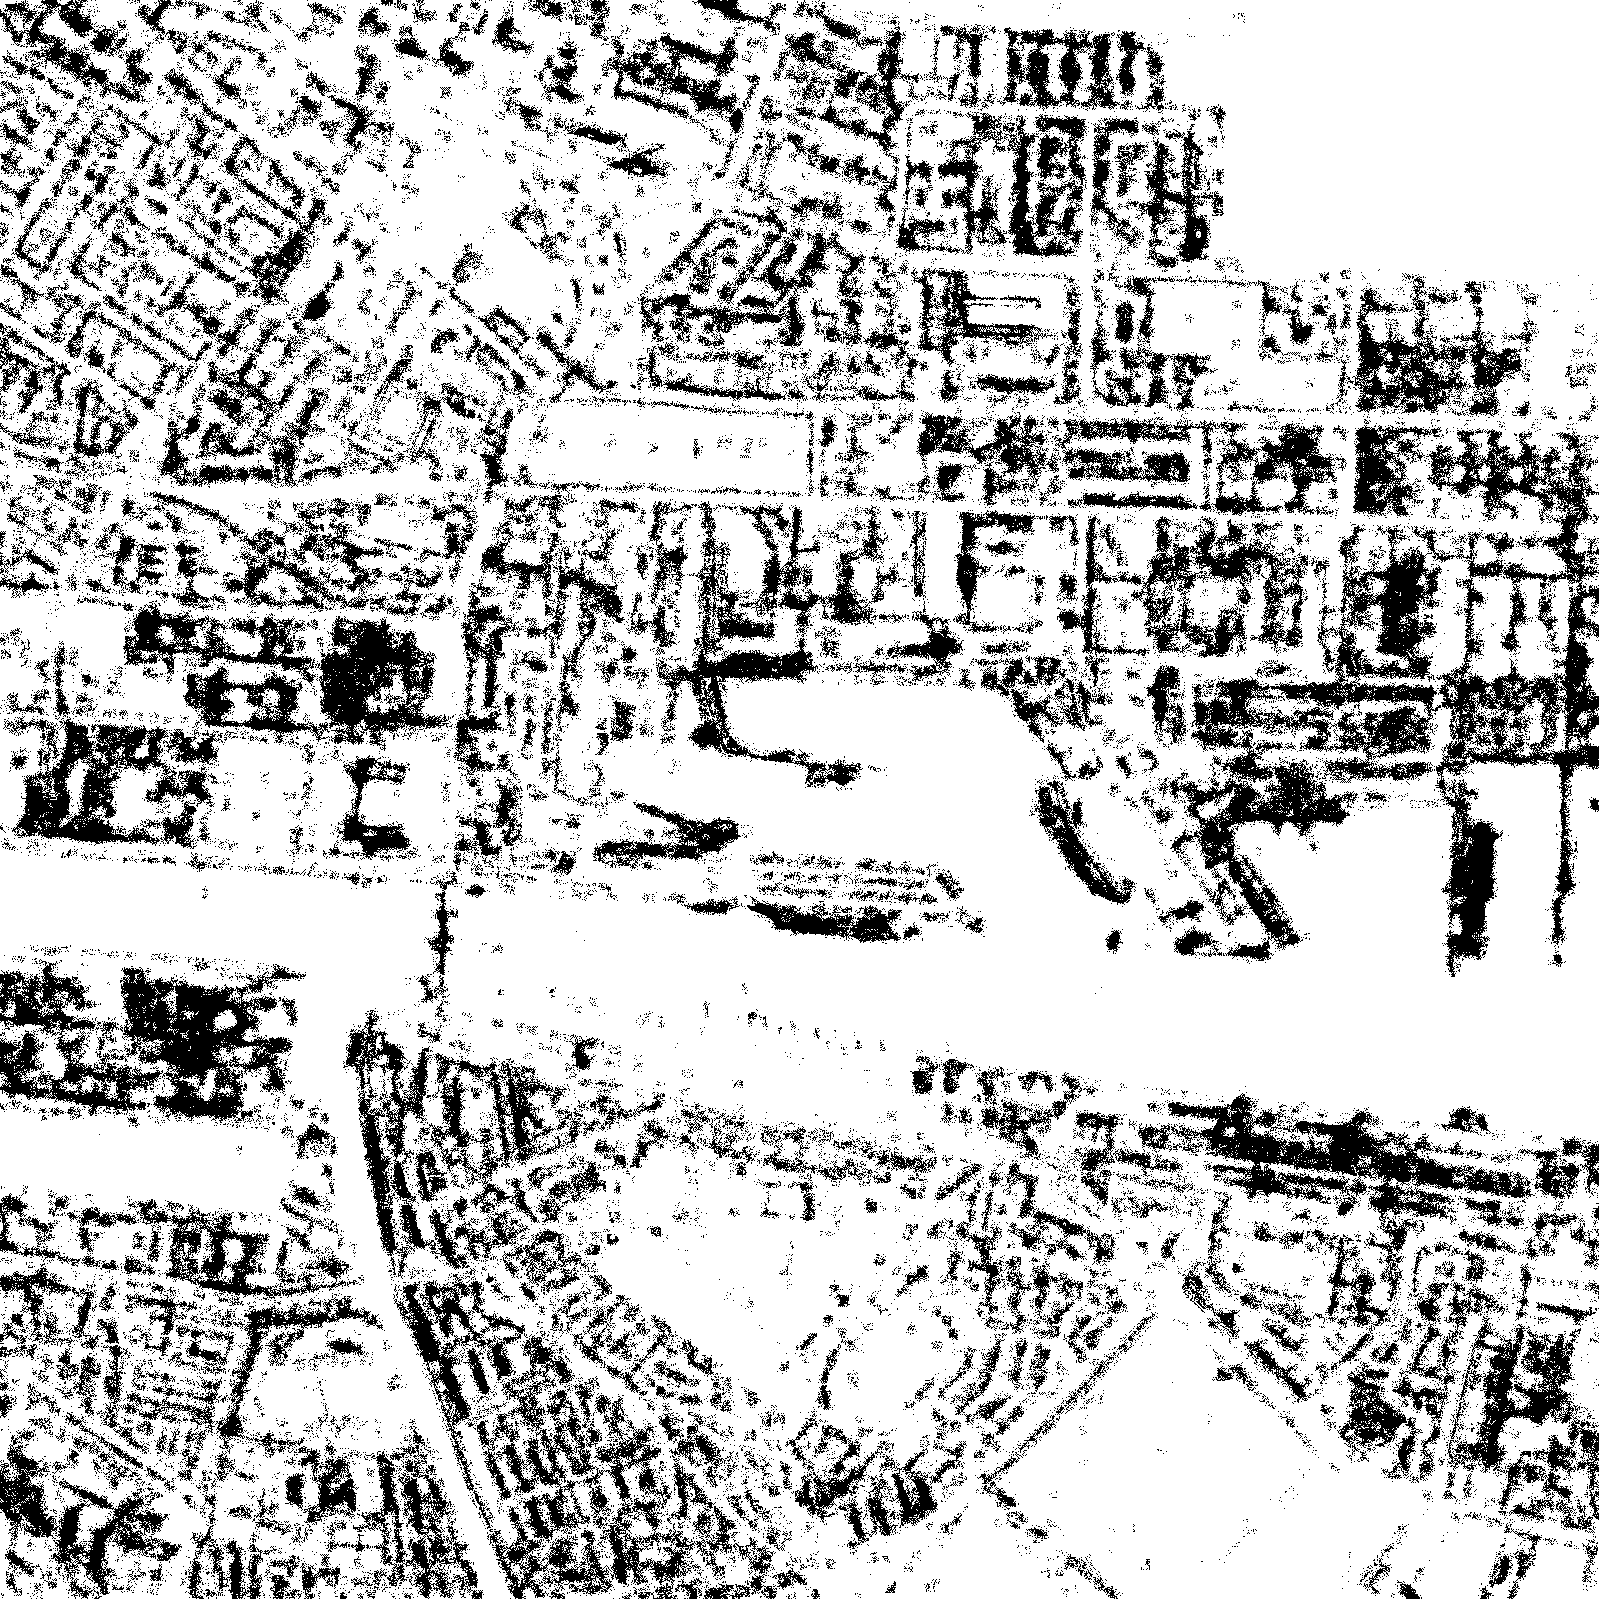
\includegraphics[width=\linewidth]{./Figures/H_005_dublin_eta4.png}
\caption{Binary map ($\eta=4$)}
\label{fig:dubc5}
\end{subfigure}

\caption{Detection of heterogeneous areas in a SAR image over Dublin Port. (a) $p$-value map with a fixed $7\times7$ window. (b–e) $p$-value maps with adaptive windows ($W_{\min}=5$, $W_{\max}=11$) for $\eta=1$--$4$. (f–j) Binary decision maps at $0.05$ significance level.}
\label{fig:dublin}
\end{figure*}

\begin{figure*}[!t]
\centering
\captionsetup{font=footnotesize}
\captionsetup[sub]{aboveskip=2pt,belowskip=2pt}

\begin{subfigure}[t]{0.19\textwidth}
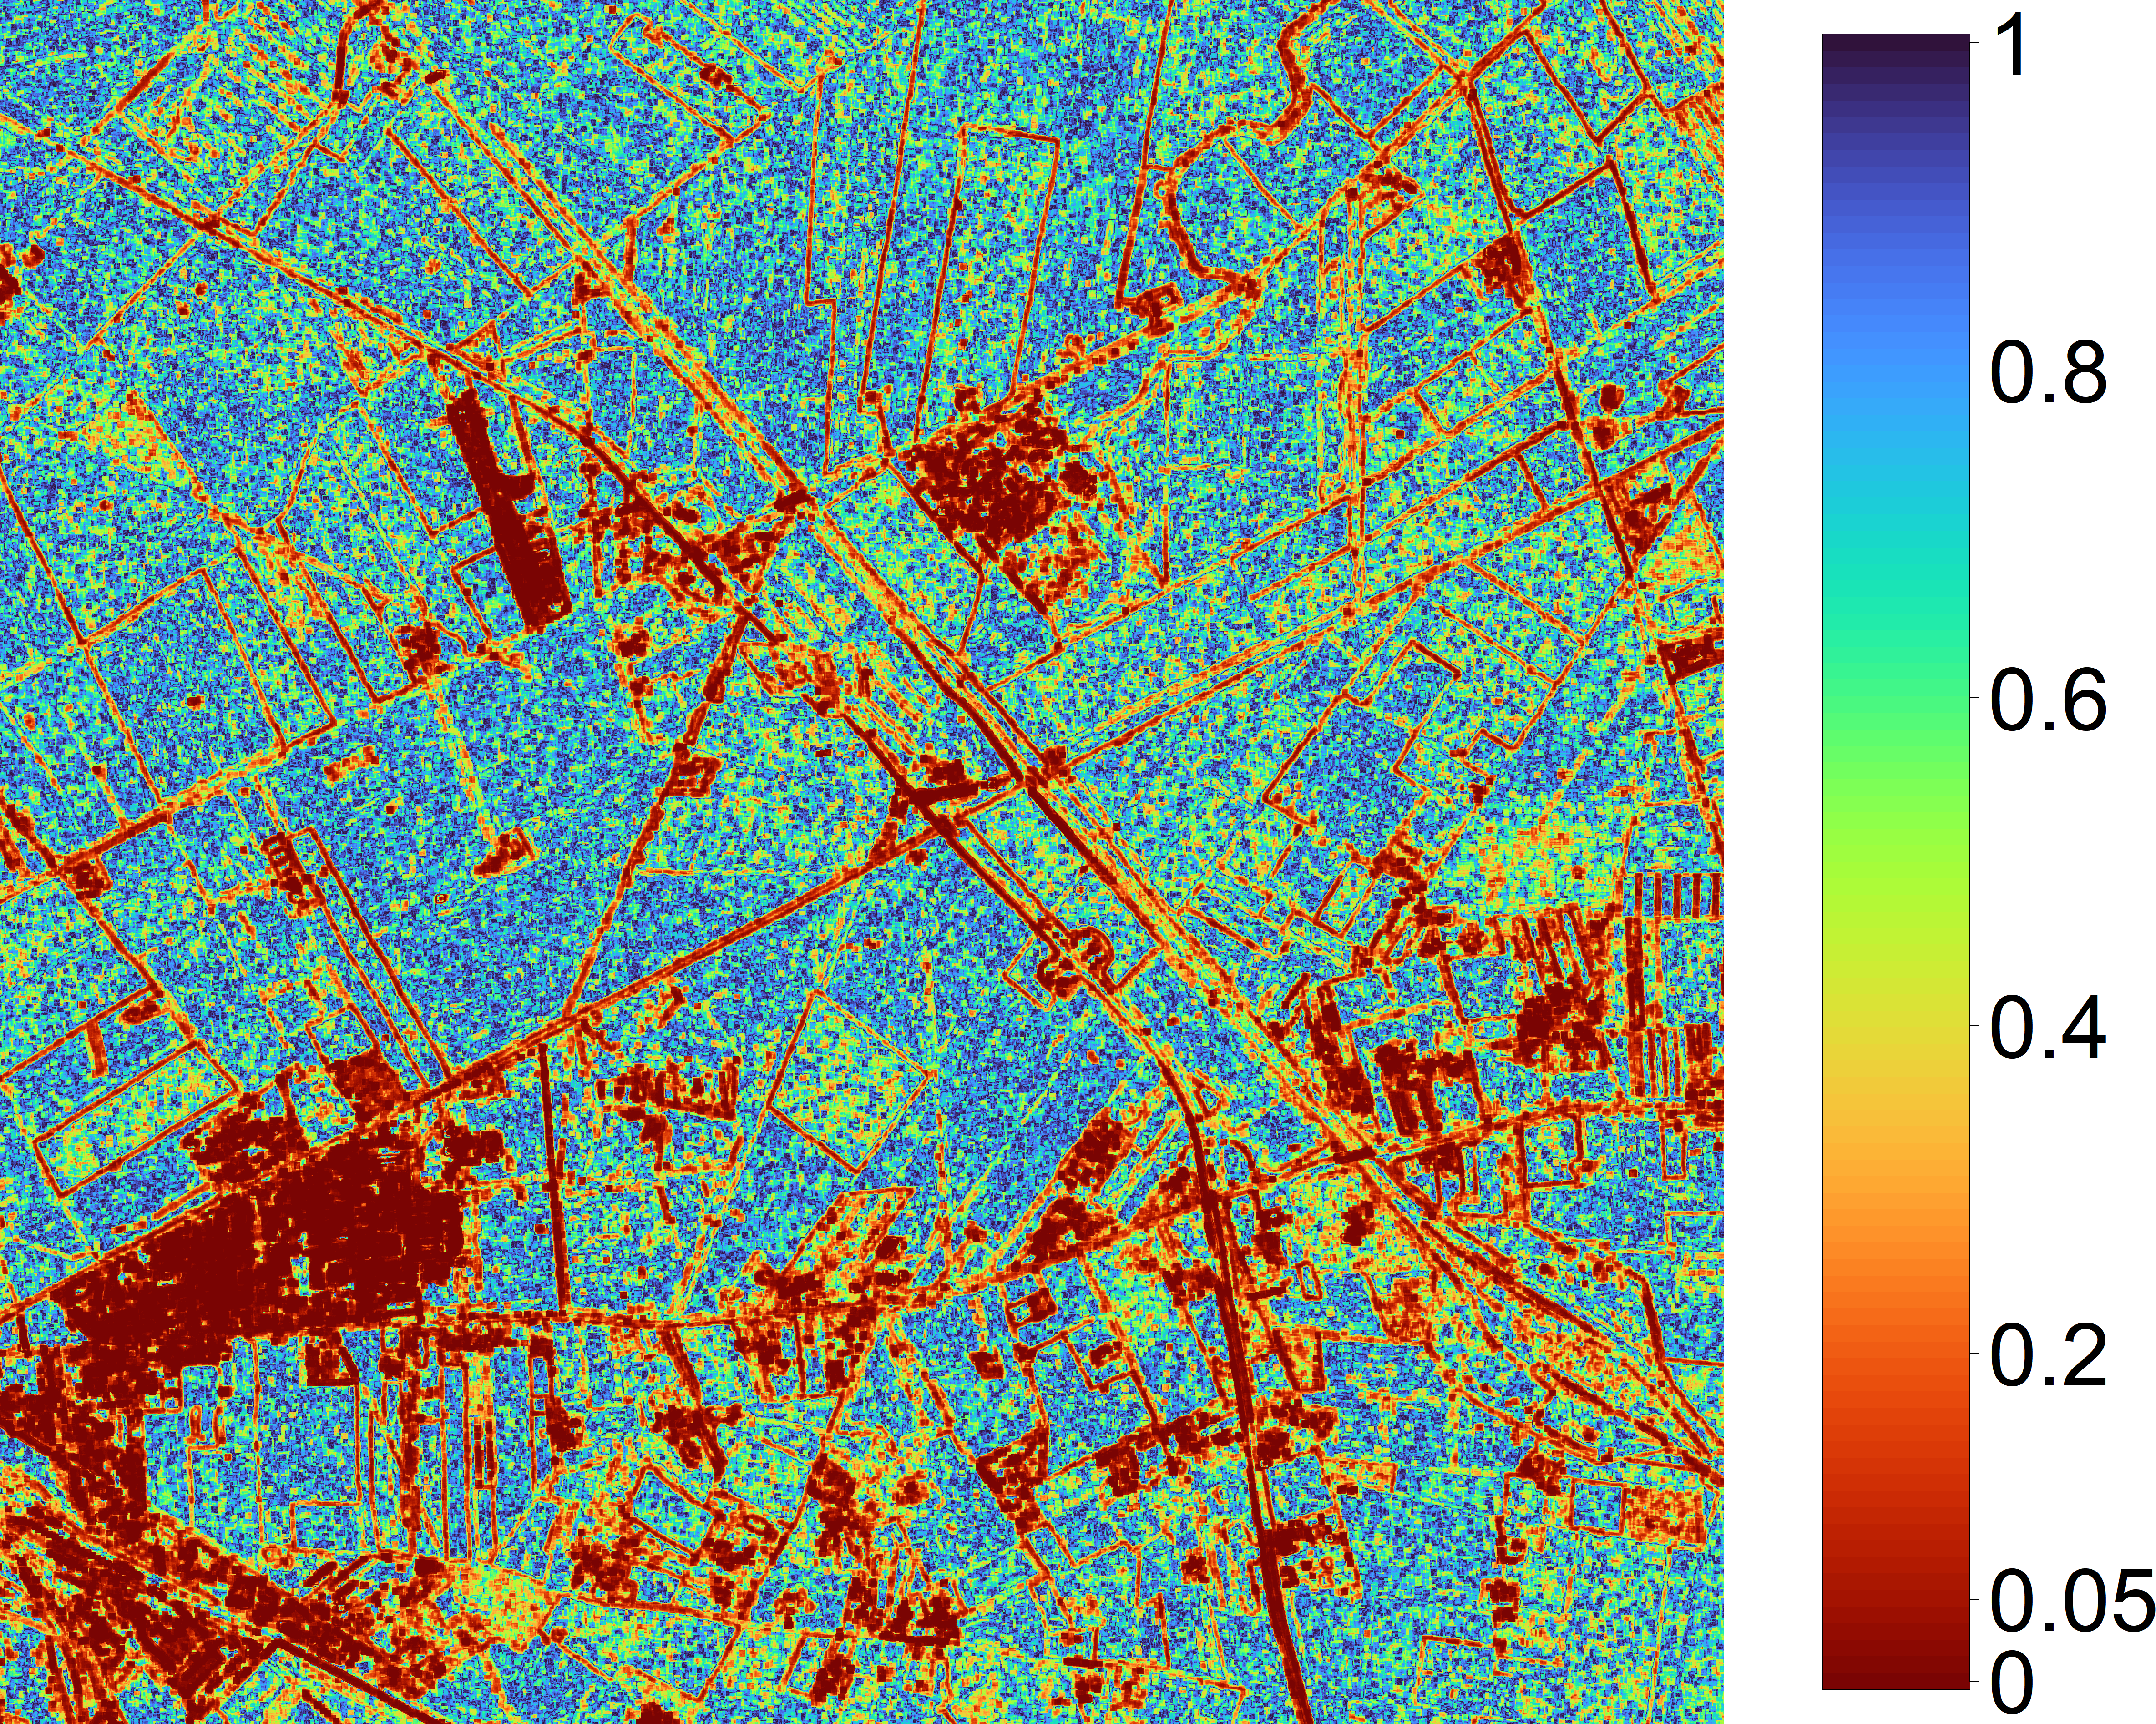
\includegraphics[width=\linewidth]{./Figures/p-values_foggia7_7.png}
\caption{$p$-value map ($7\times7$)}
\label{fig:foc1}
\end{subfigure}\hfill
\begin{subfigure}[t]{0.19\textwidth}
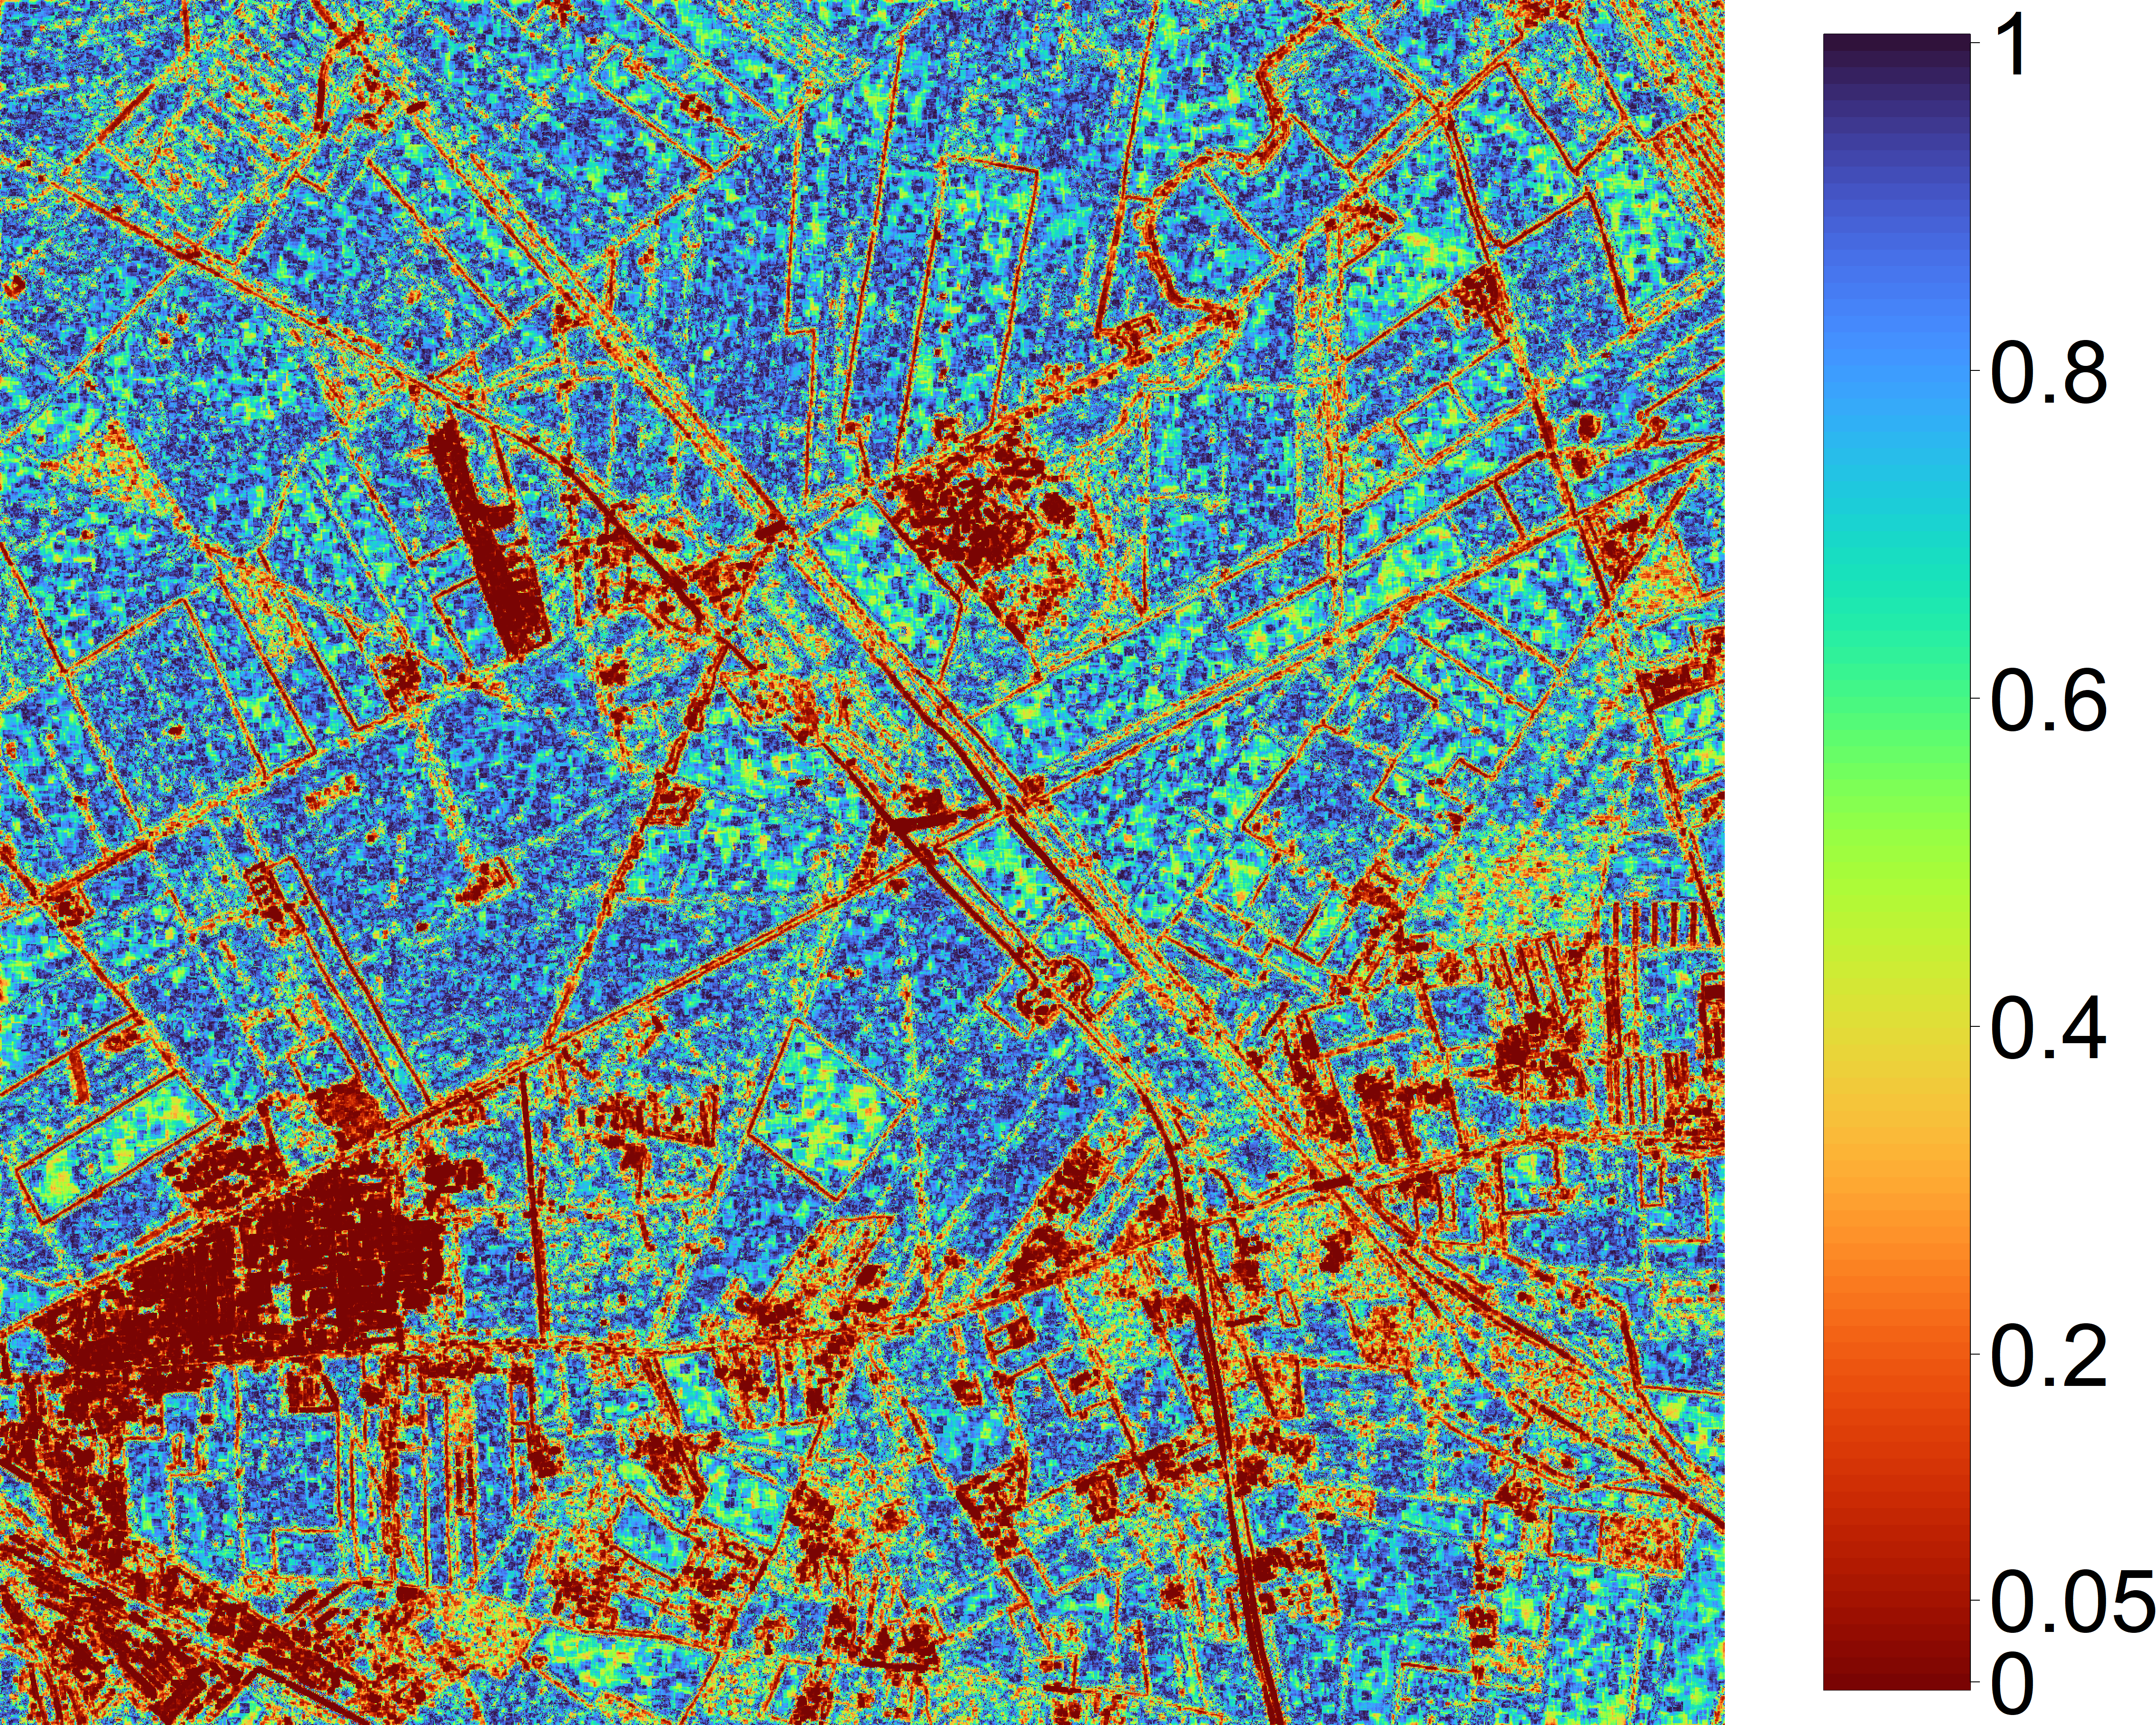
\includegraphics[width=\linewidth]{./Figures/p-values_FoggiaL24_eta_1.00_5x11_B100_lambda_085.png}
\caption{$p$-value map ($\eta=1$)}
\label{fig:foc2}
\end{subfigure}\hfill
\begin{subfigure}[t]{0.19\textwidth}
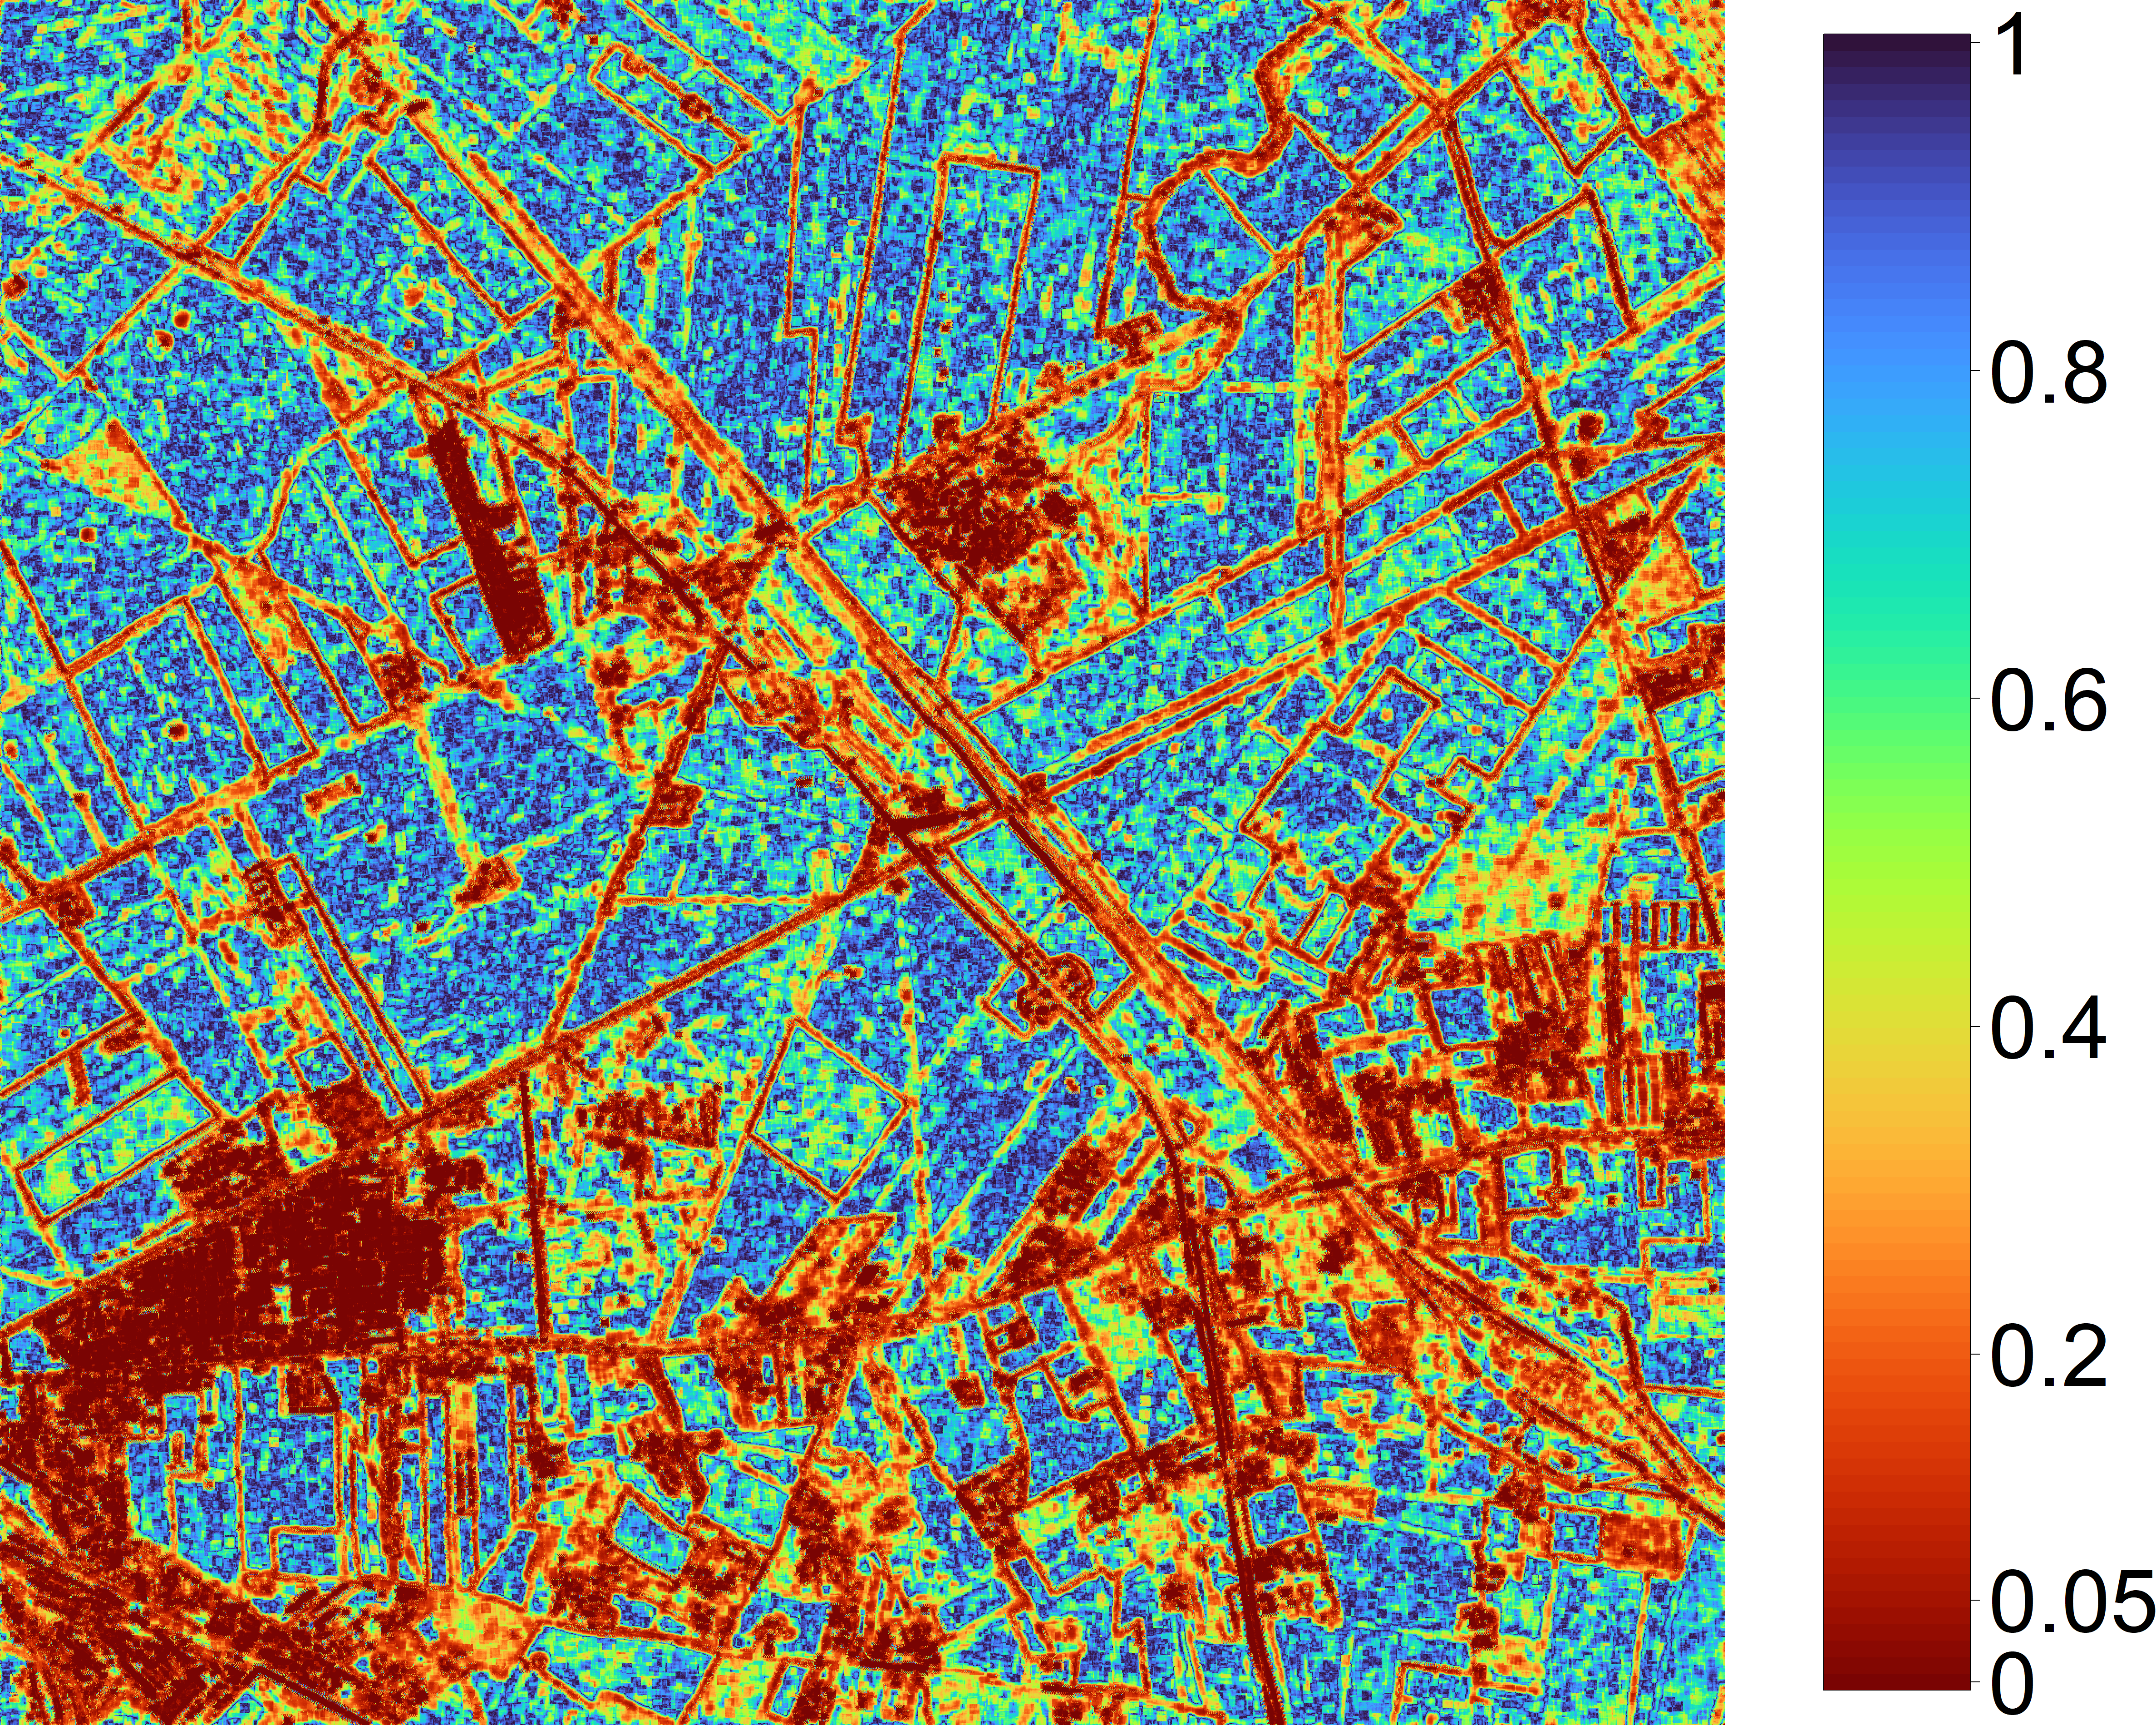
\includegraphics[width=\linewidth]{./Figures/p-values_FoggiaL24_eta_2.00_5x11_B100_lambda_0852.png}
\caption{$p$-value map ($\eta=2$)}
\label{fig:foc3}
\end{subfigure}\hfill
\begin{subfigure}[t]{0.19\textwidth}
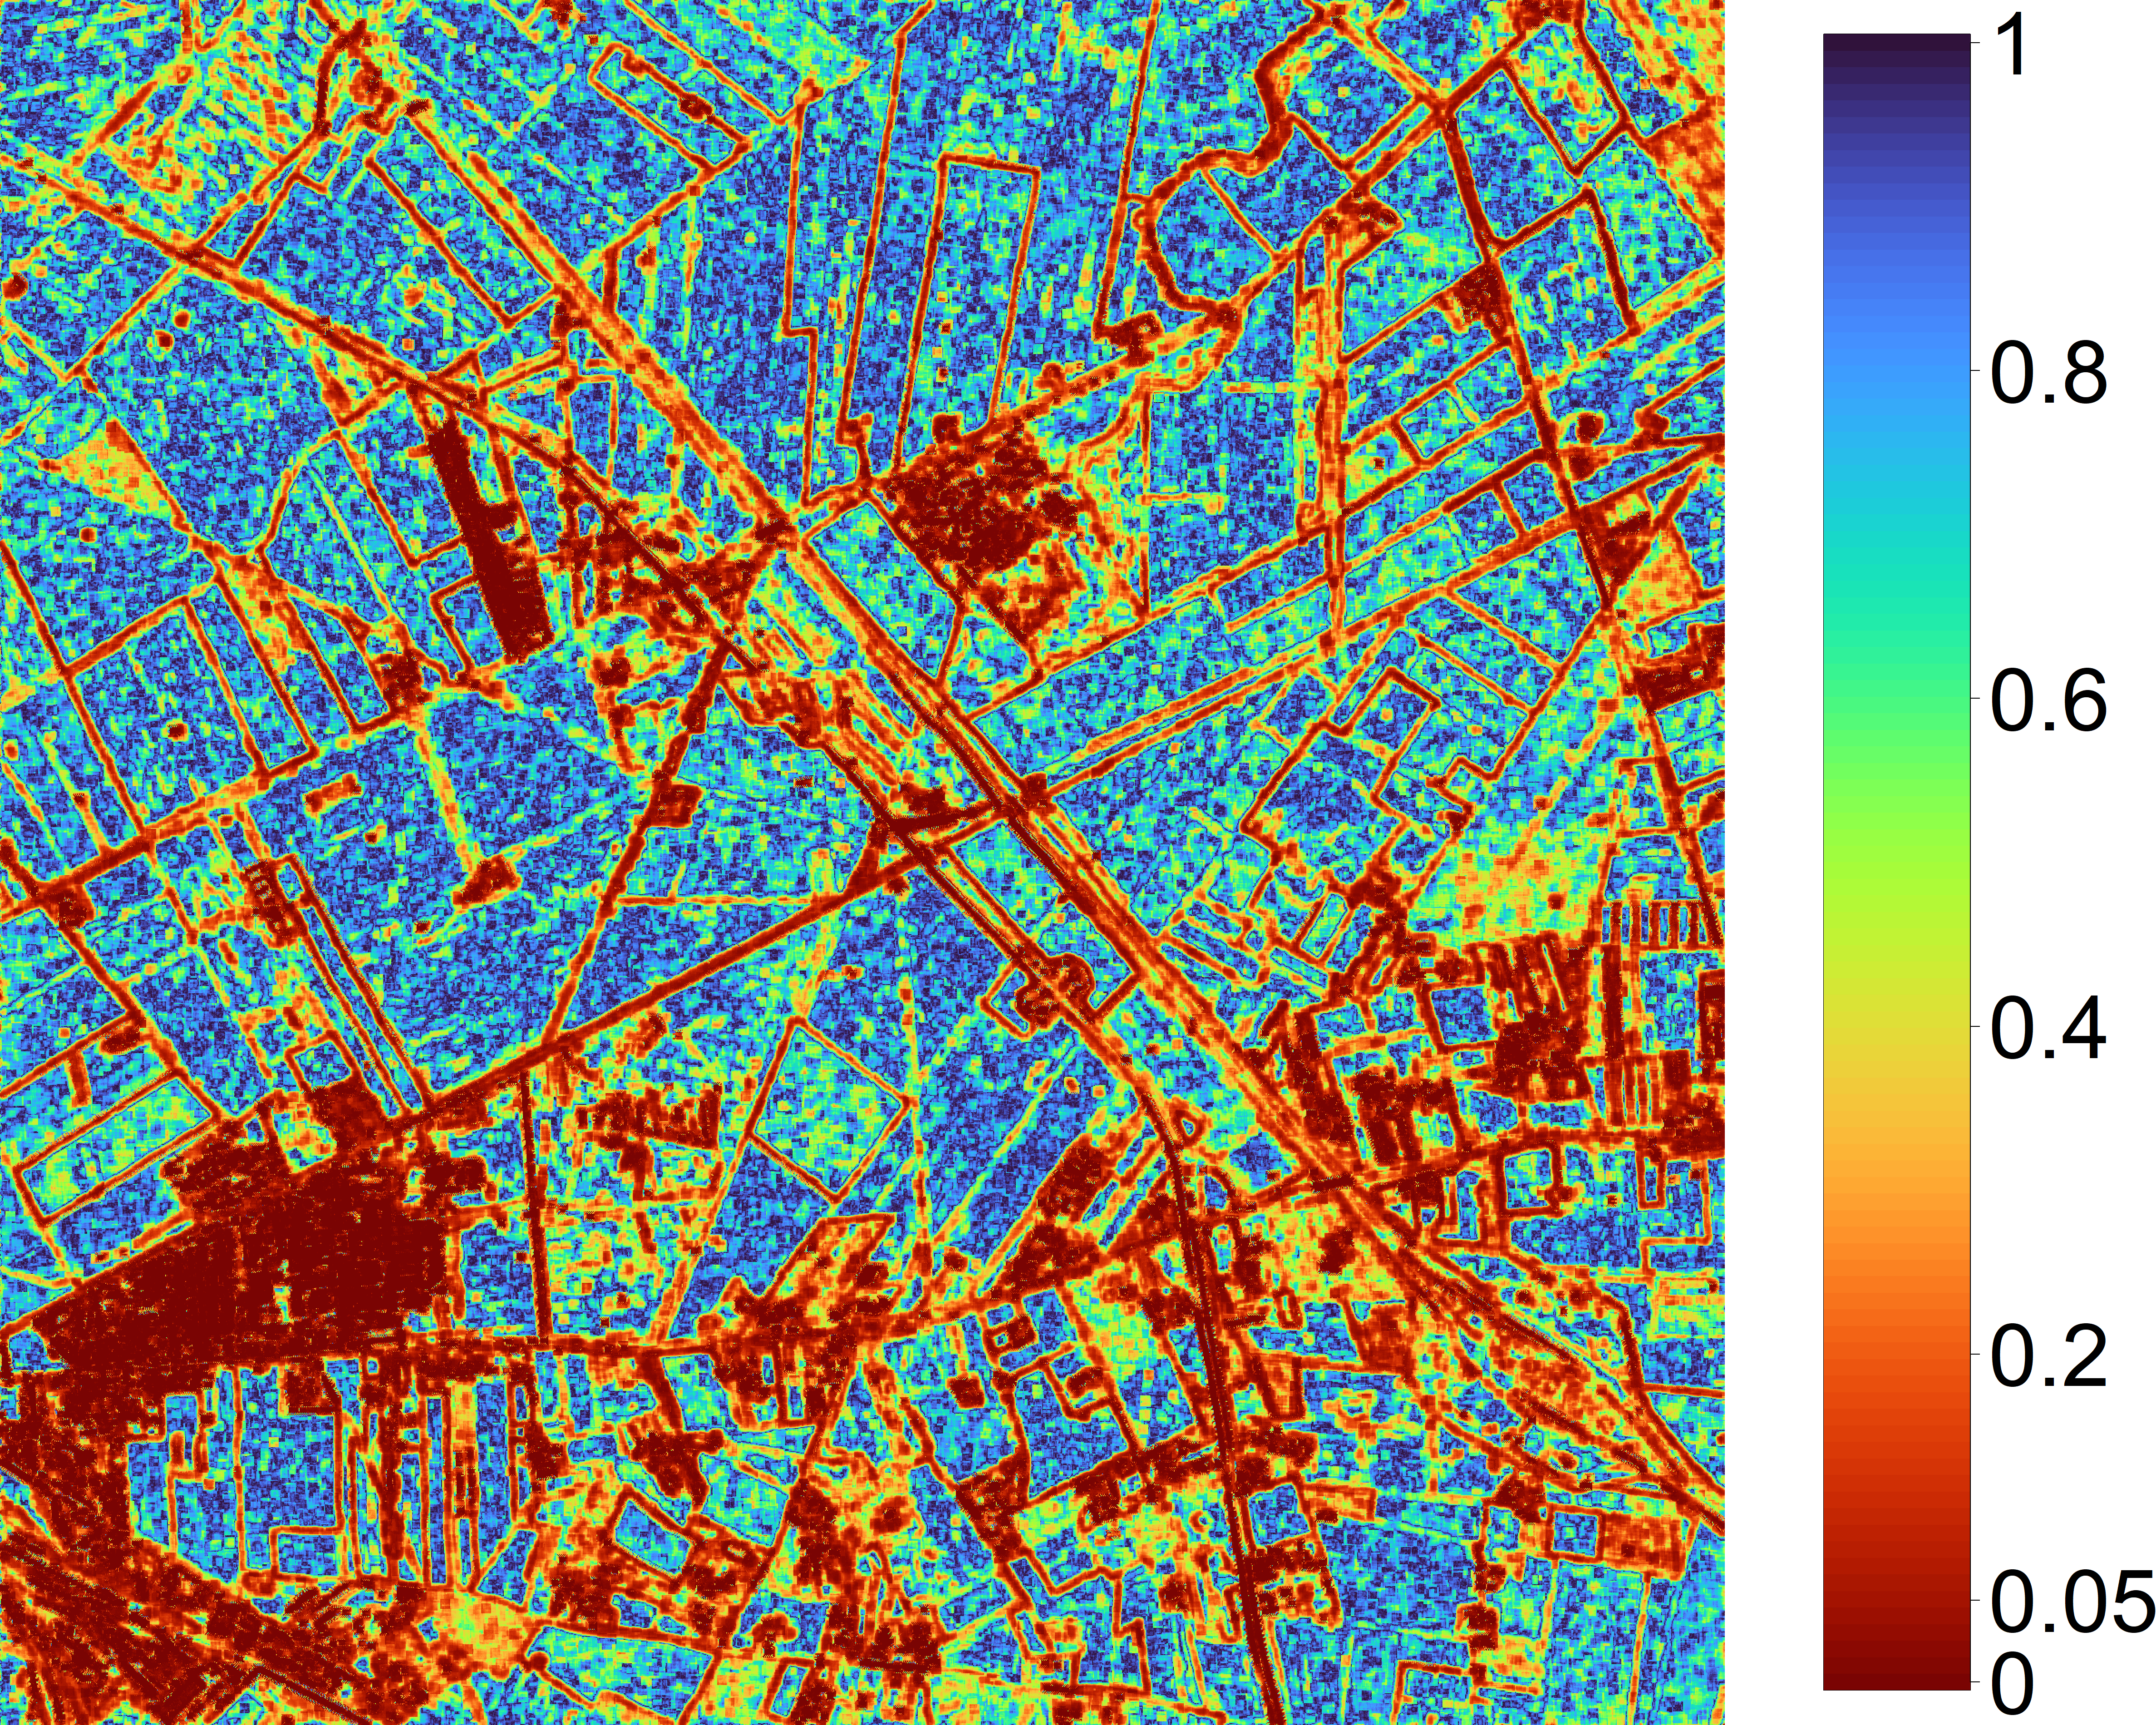
\includegraphics[width=\linewidth]{./Figures/p-values_FoggiaL24_eta_3.0n_5x11_B100_lambda_085.png}
\caption{$p$-value map ($\eta=3$)}
\label{fig:foc4}
\end{subfigure}\hfill
\begin{subfigure}[t]{0.19\textwidth}
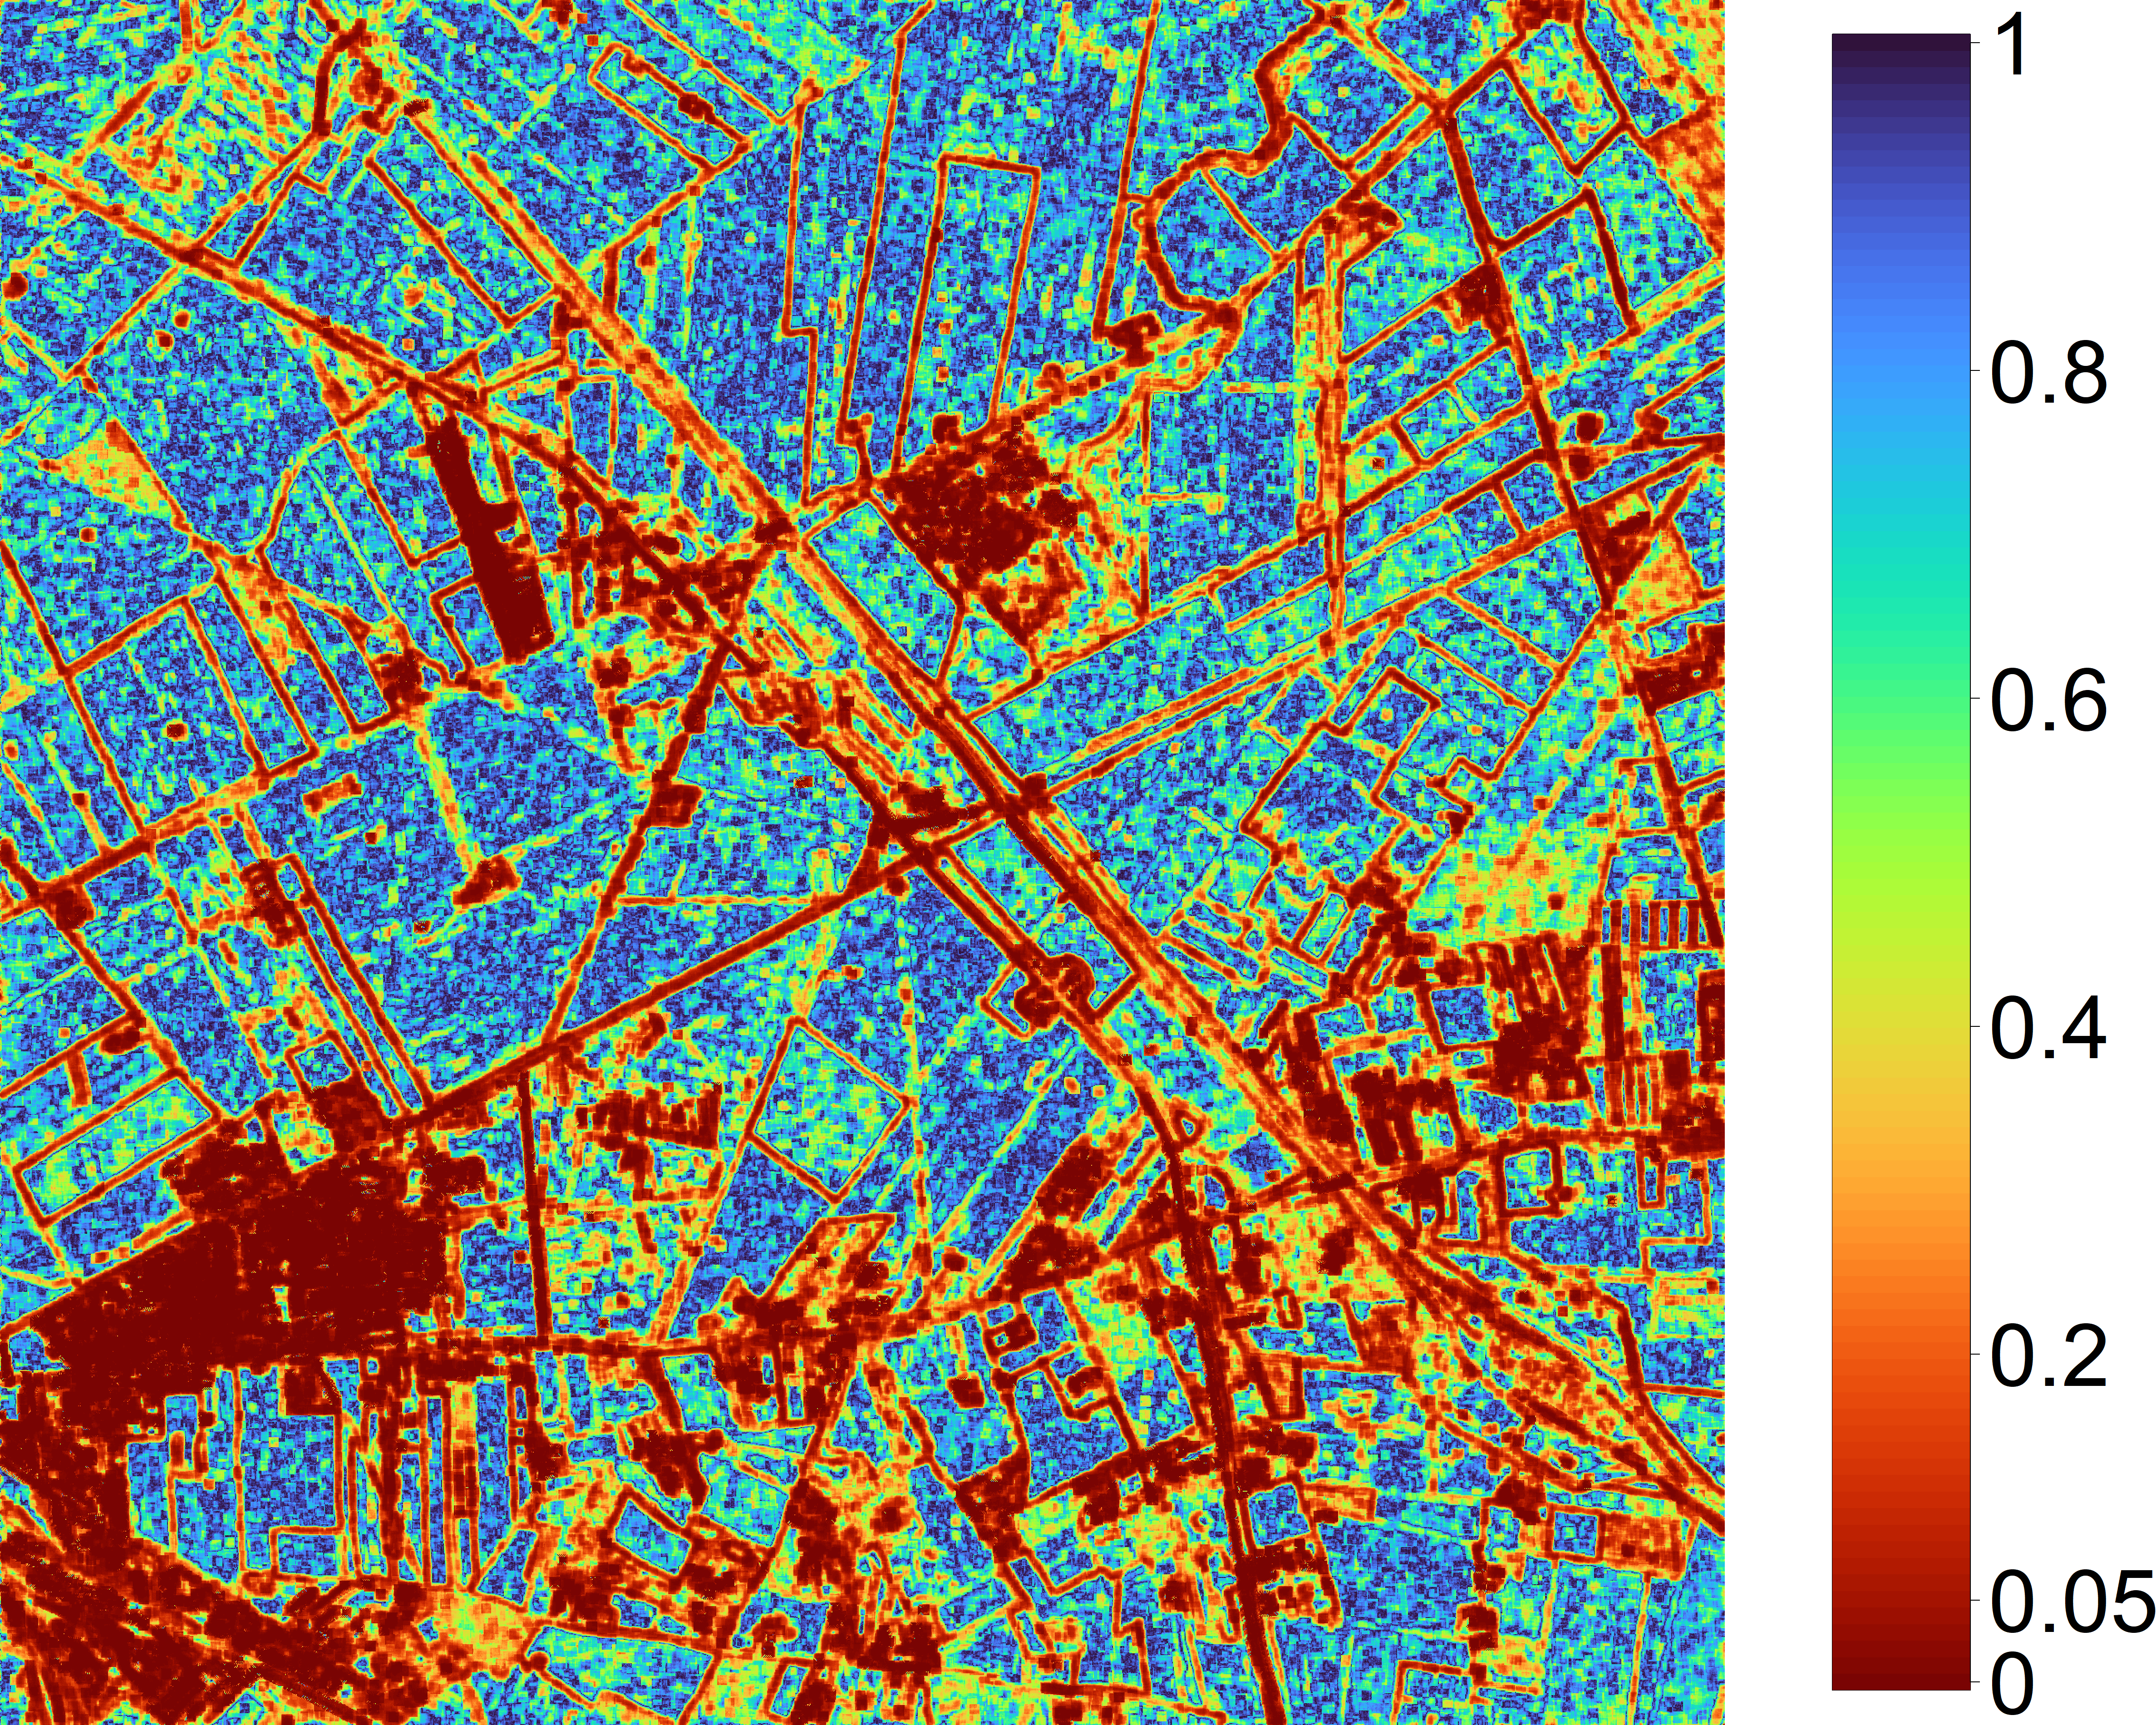
\includegraphics[width=\linewidth]{./Figures/p-values_Foggia_eta4.png}
\caption{$p$-value map ($\eta=4$)}
\label{fig:foc5}
\end{subfigure}

\vspace{4pt}

\begin{subfigure}[t]{0.18\textwidth}
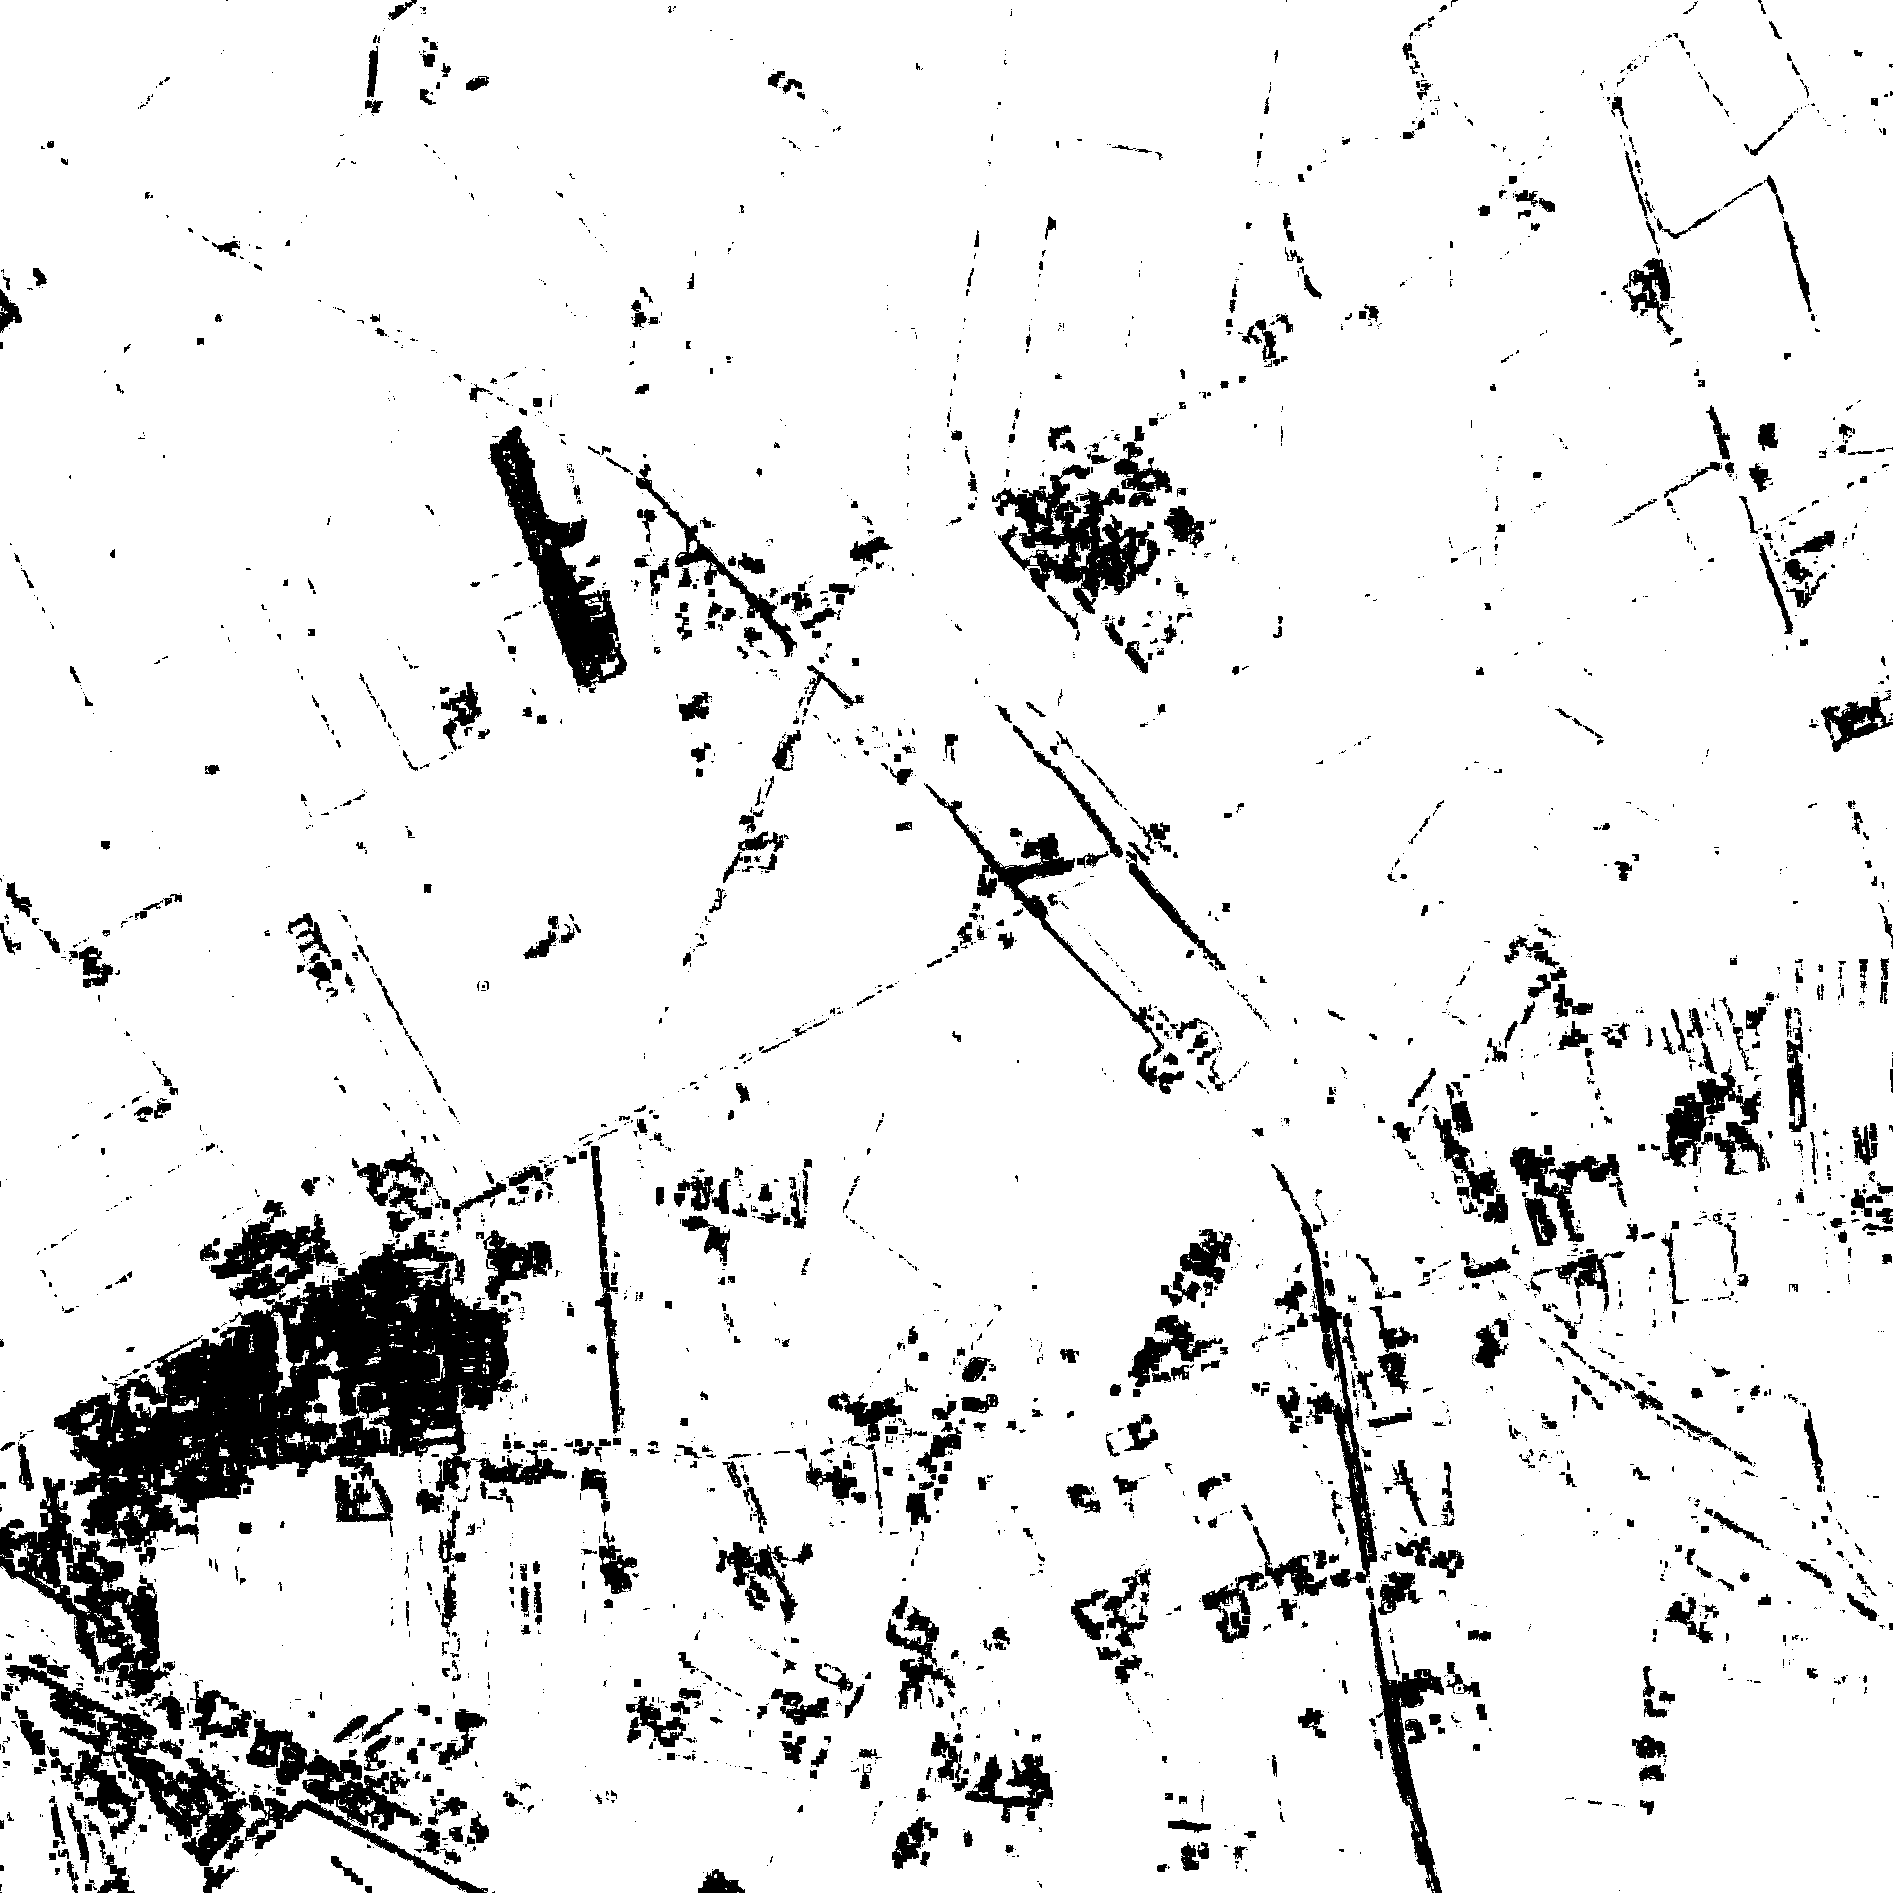
\includegraphics[width=\linewidth]{./Figures/H_005_fogia_7x7.png}
\caption{Binary map ($7\times7$)}
\label{fig:fogc1}
\end{subfigure}\hfill
\begin{subfigure}[t]{0.18\textwidth}
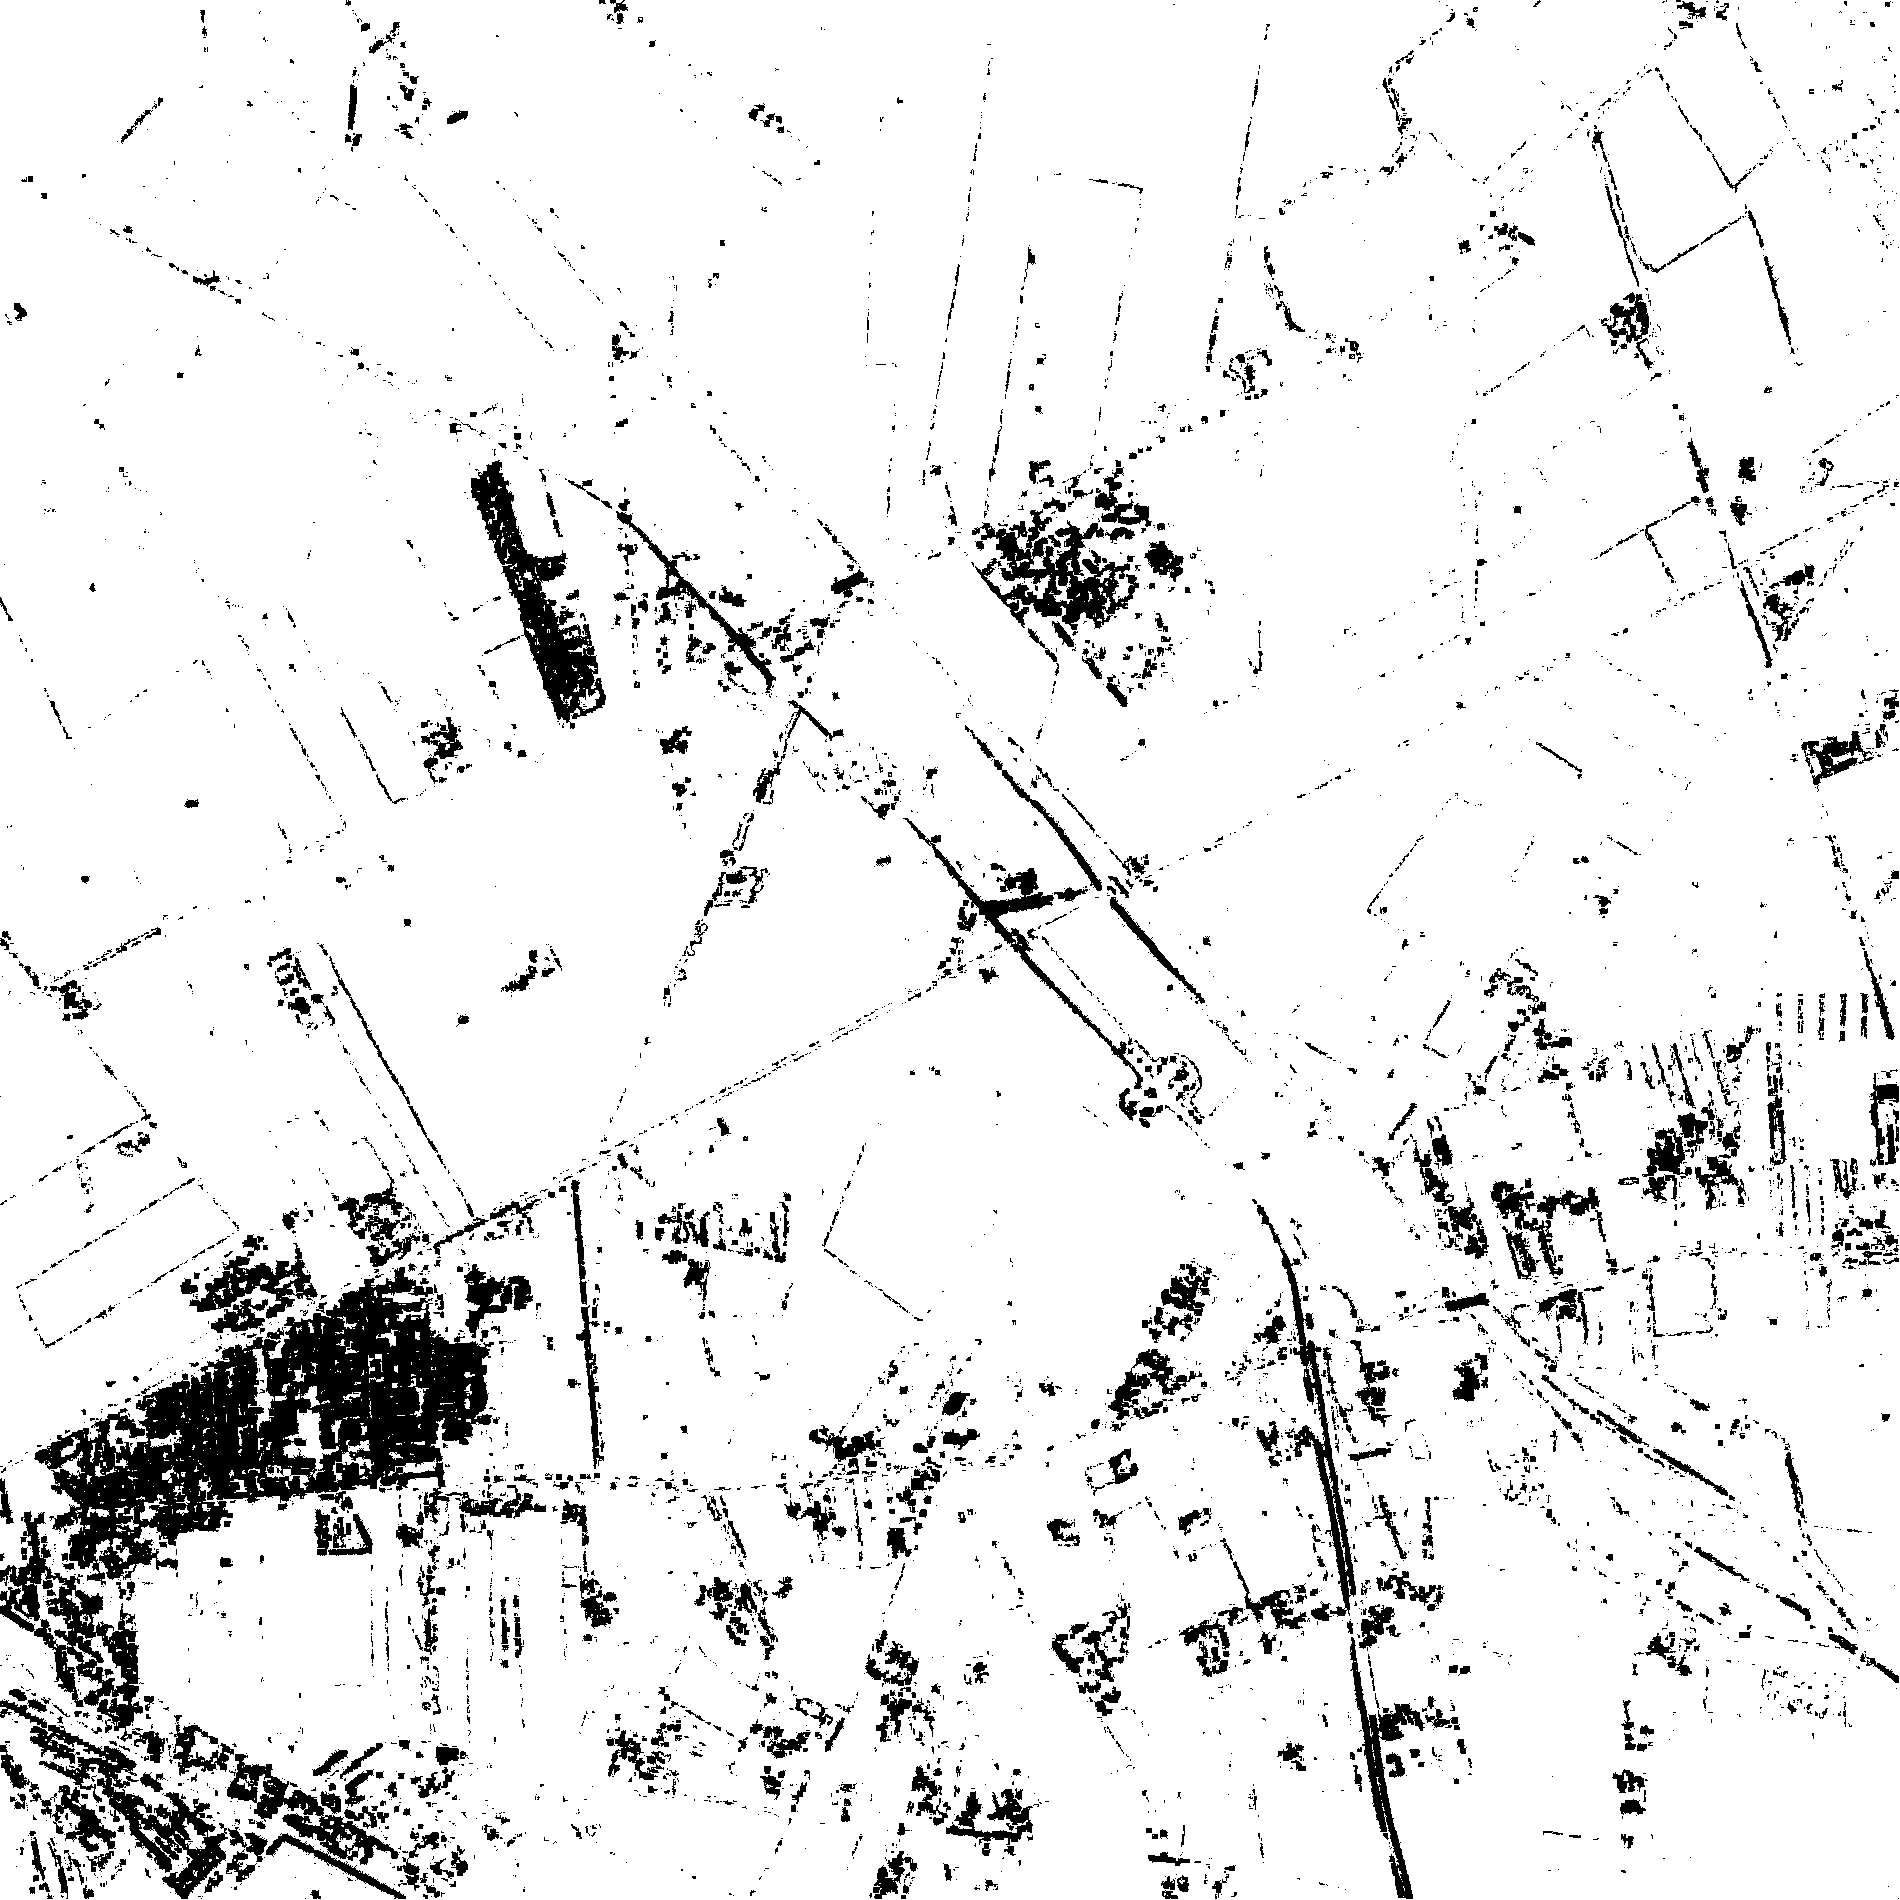
\includegraphics[width=\linewidth]{./Figures/H_005_FoggiaL24_eta_1.00_5x11_B100_lambda_081.png}
\caption{Binary map ($\eta=1$)}
\label{fig:fogc2}
\end{subfigure}\hfill
\begin{subfigure}[t]{0.18\textwidth}
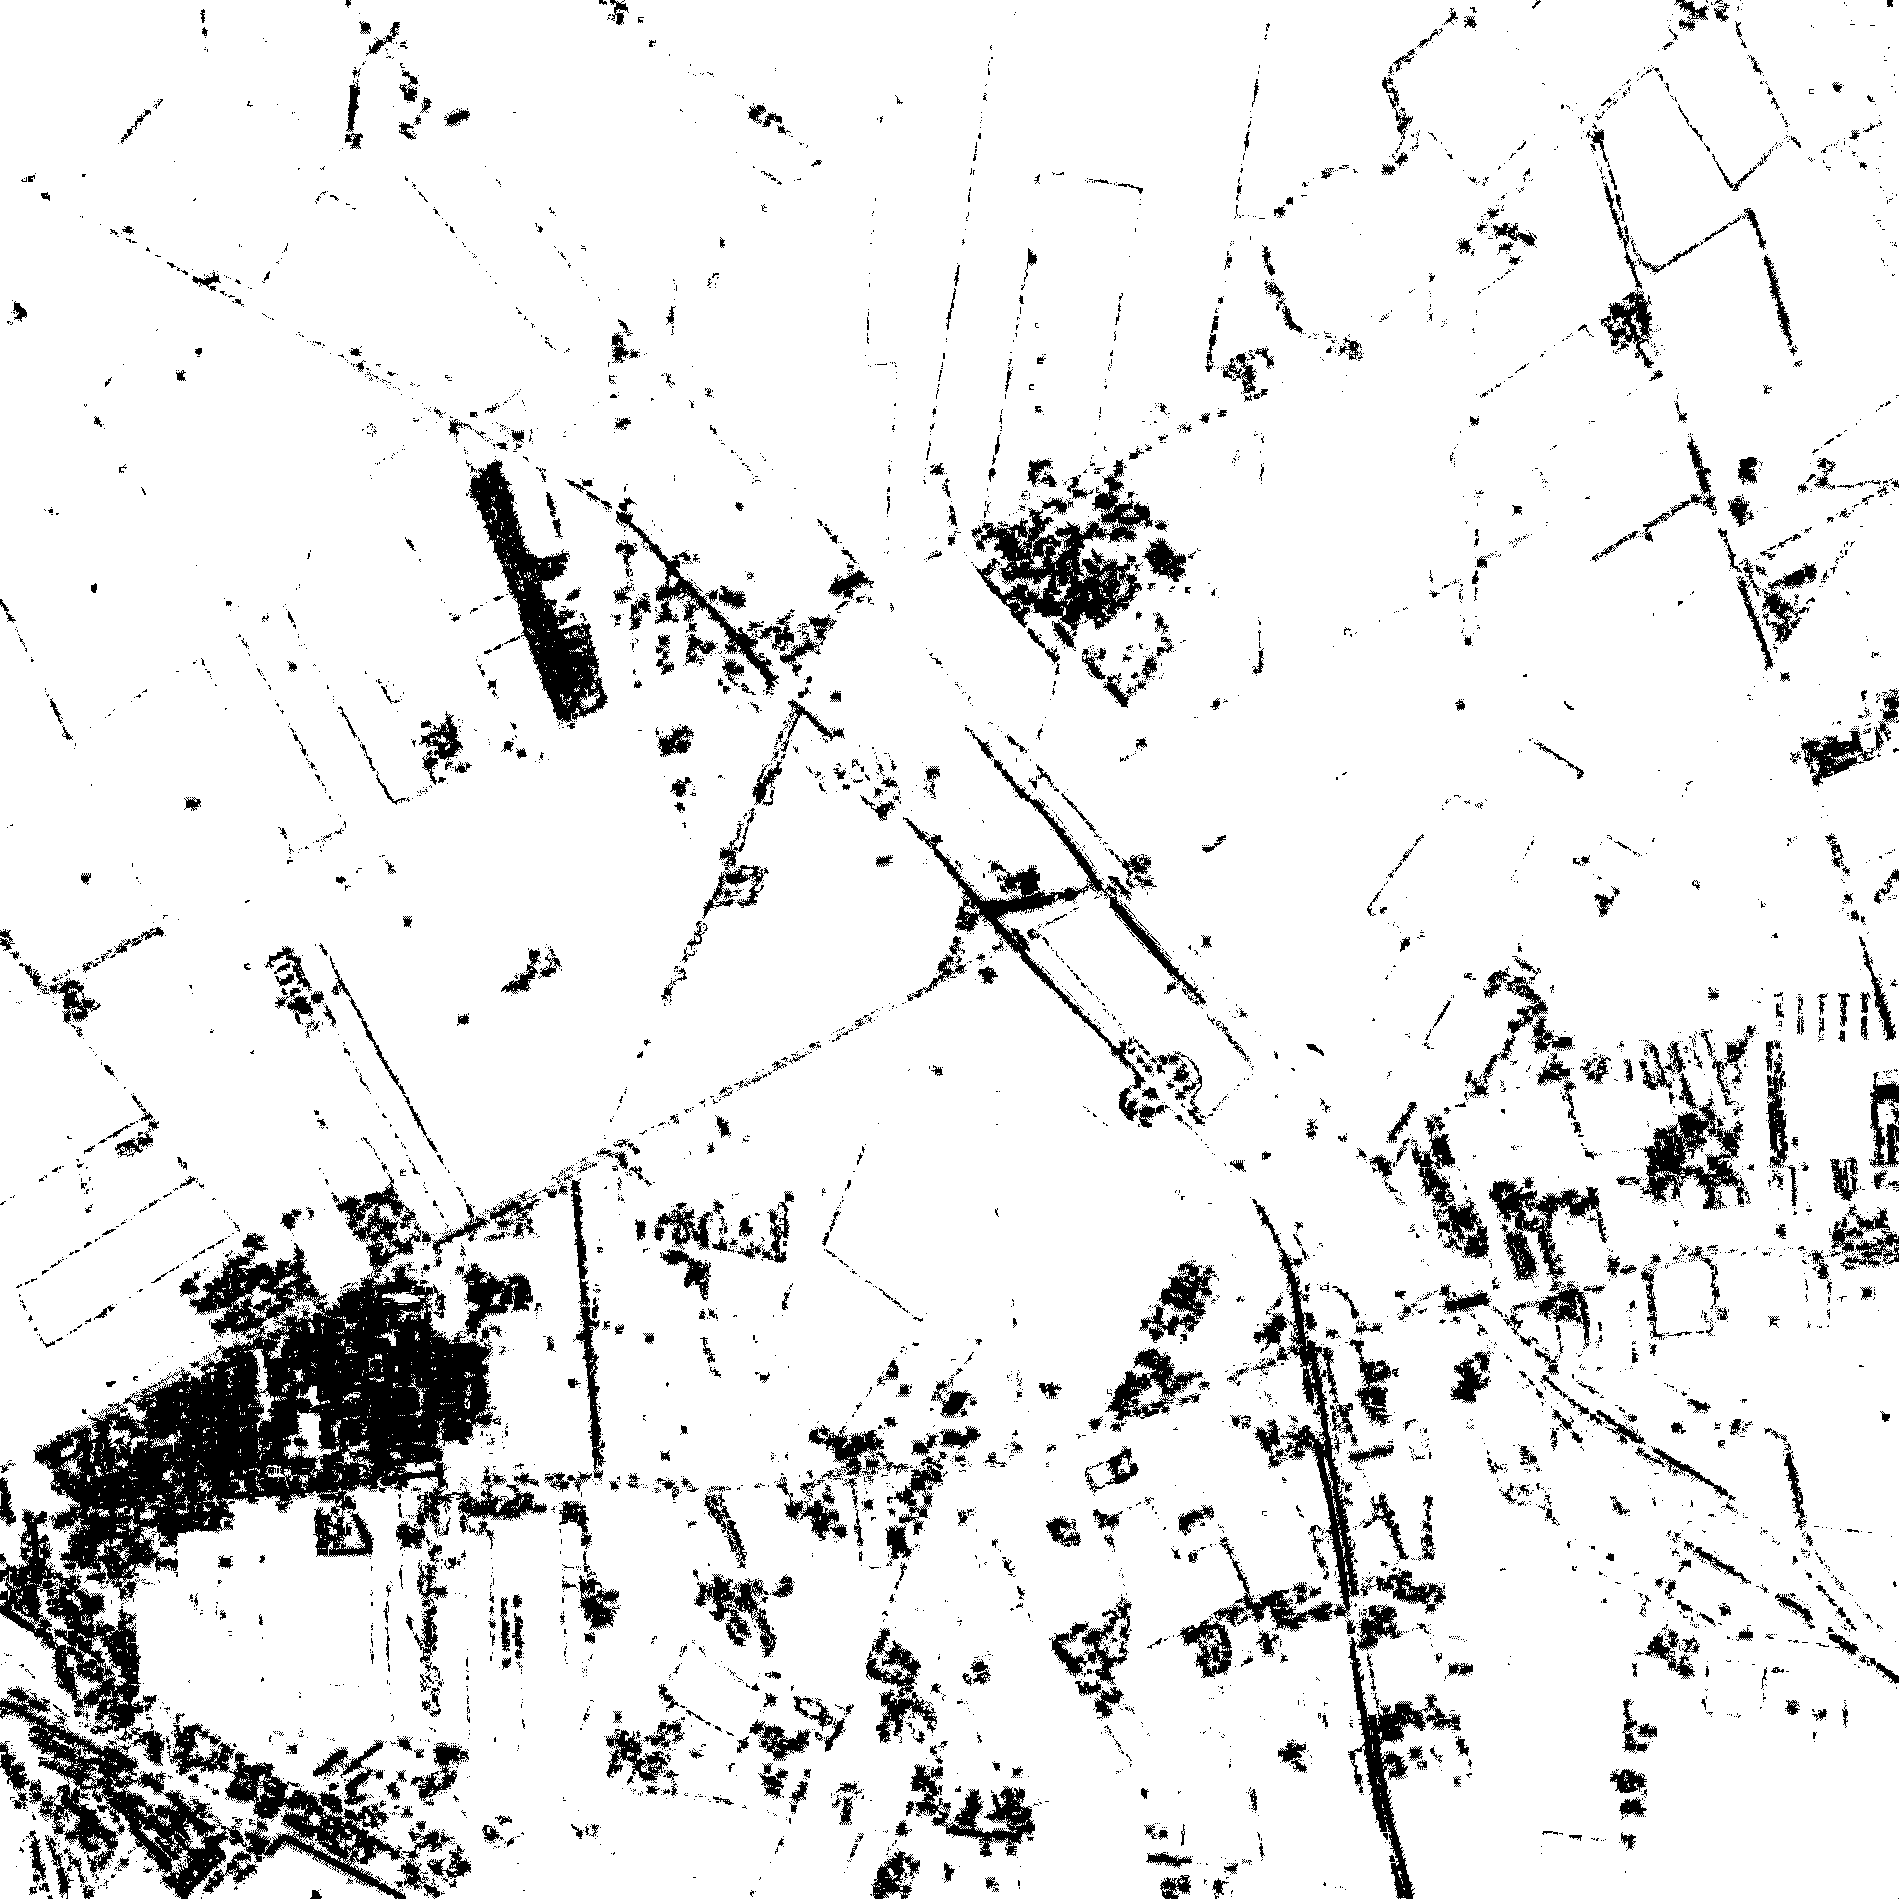
\includegraphics[width=\linewidth]{./Figures/H_005_FoggiaL24_eta_2.00_5x11_B100_lambda_085.png}
\caption{Binary map ($\eta=2$)}
\label{fig:fogc3}
\end{subfigure}\hfill
\begin{subfigure}[t]{0.18\textwidth}
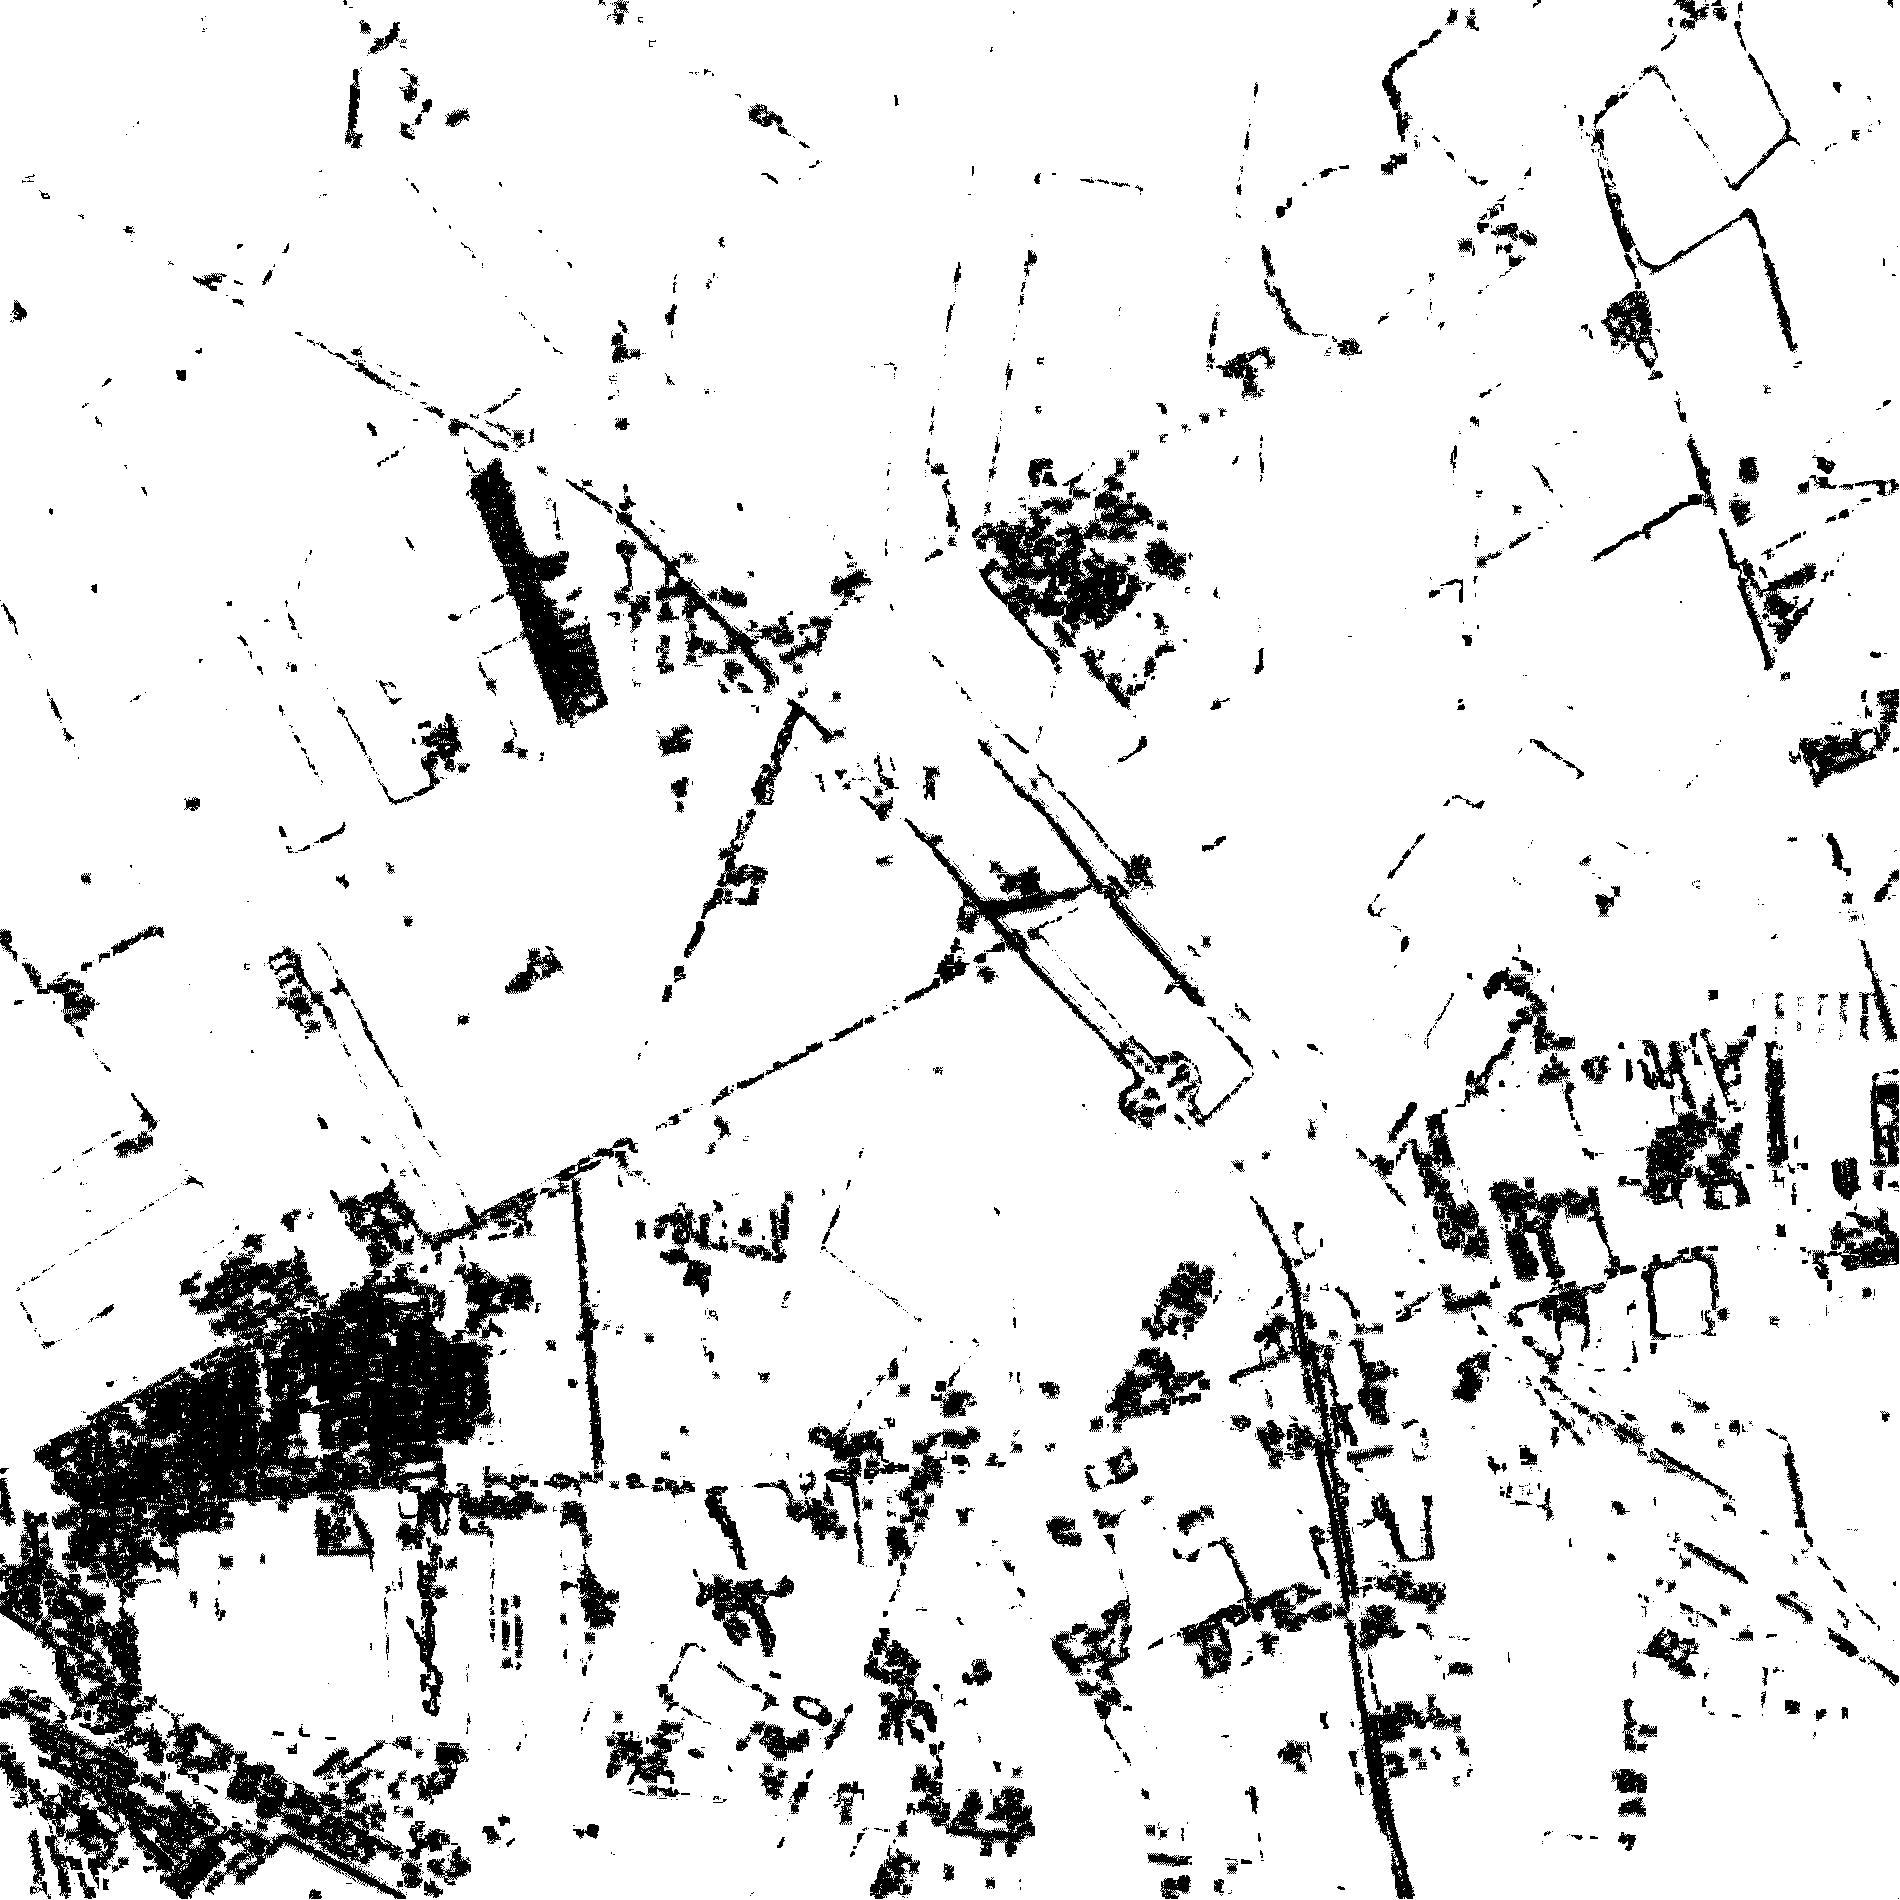
\includegraphics[width=\linewidth]{./Figures/H_005_FoggiaL24_eta_3.0n_5x11_B100_lambda_081.png}
\caption{Binary map ($\eta=3$)}
\label{fig:fogc4}
\end{subfigure}\hfill
\begin{subfigure}[t]{0.18\textwidth}
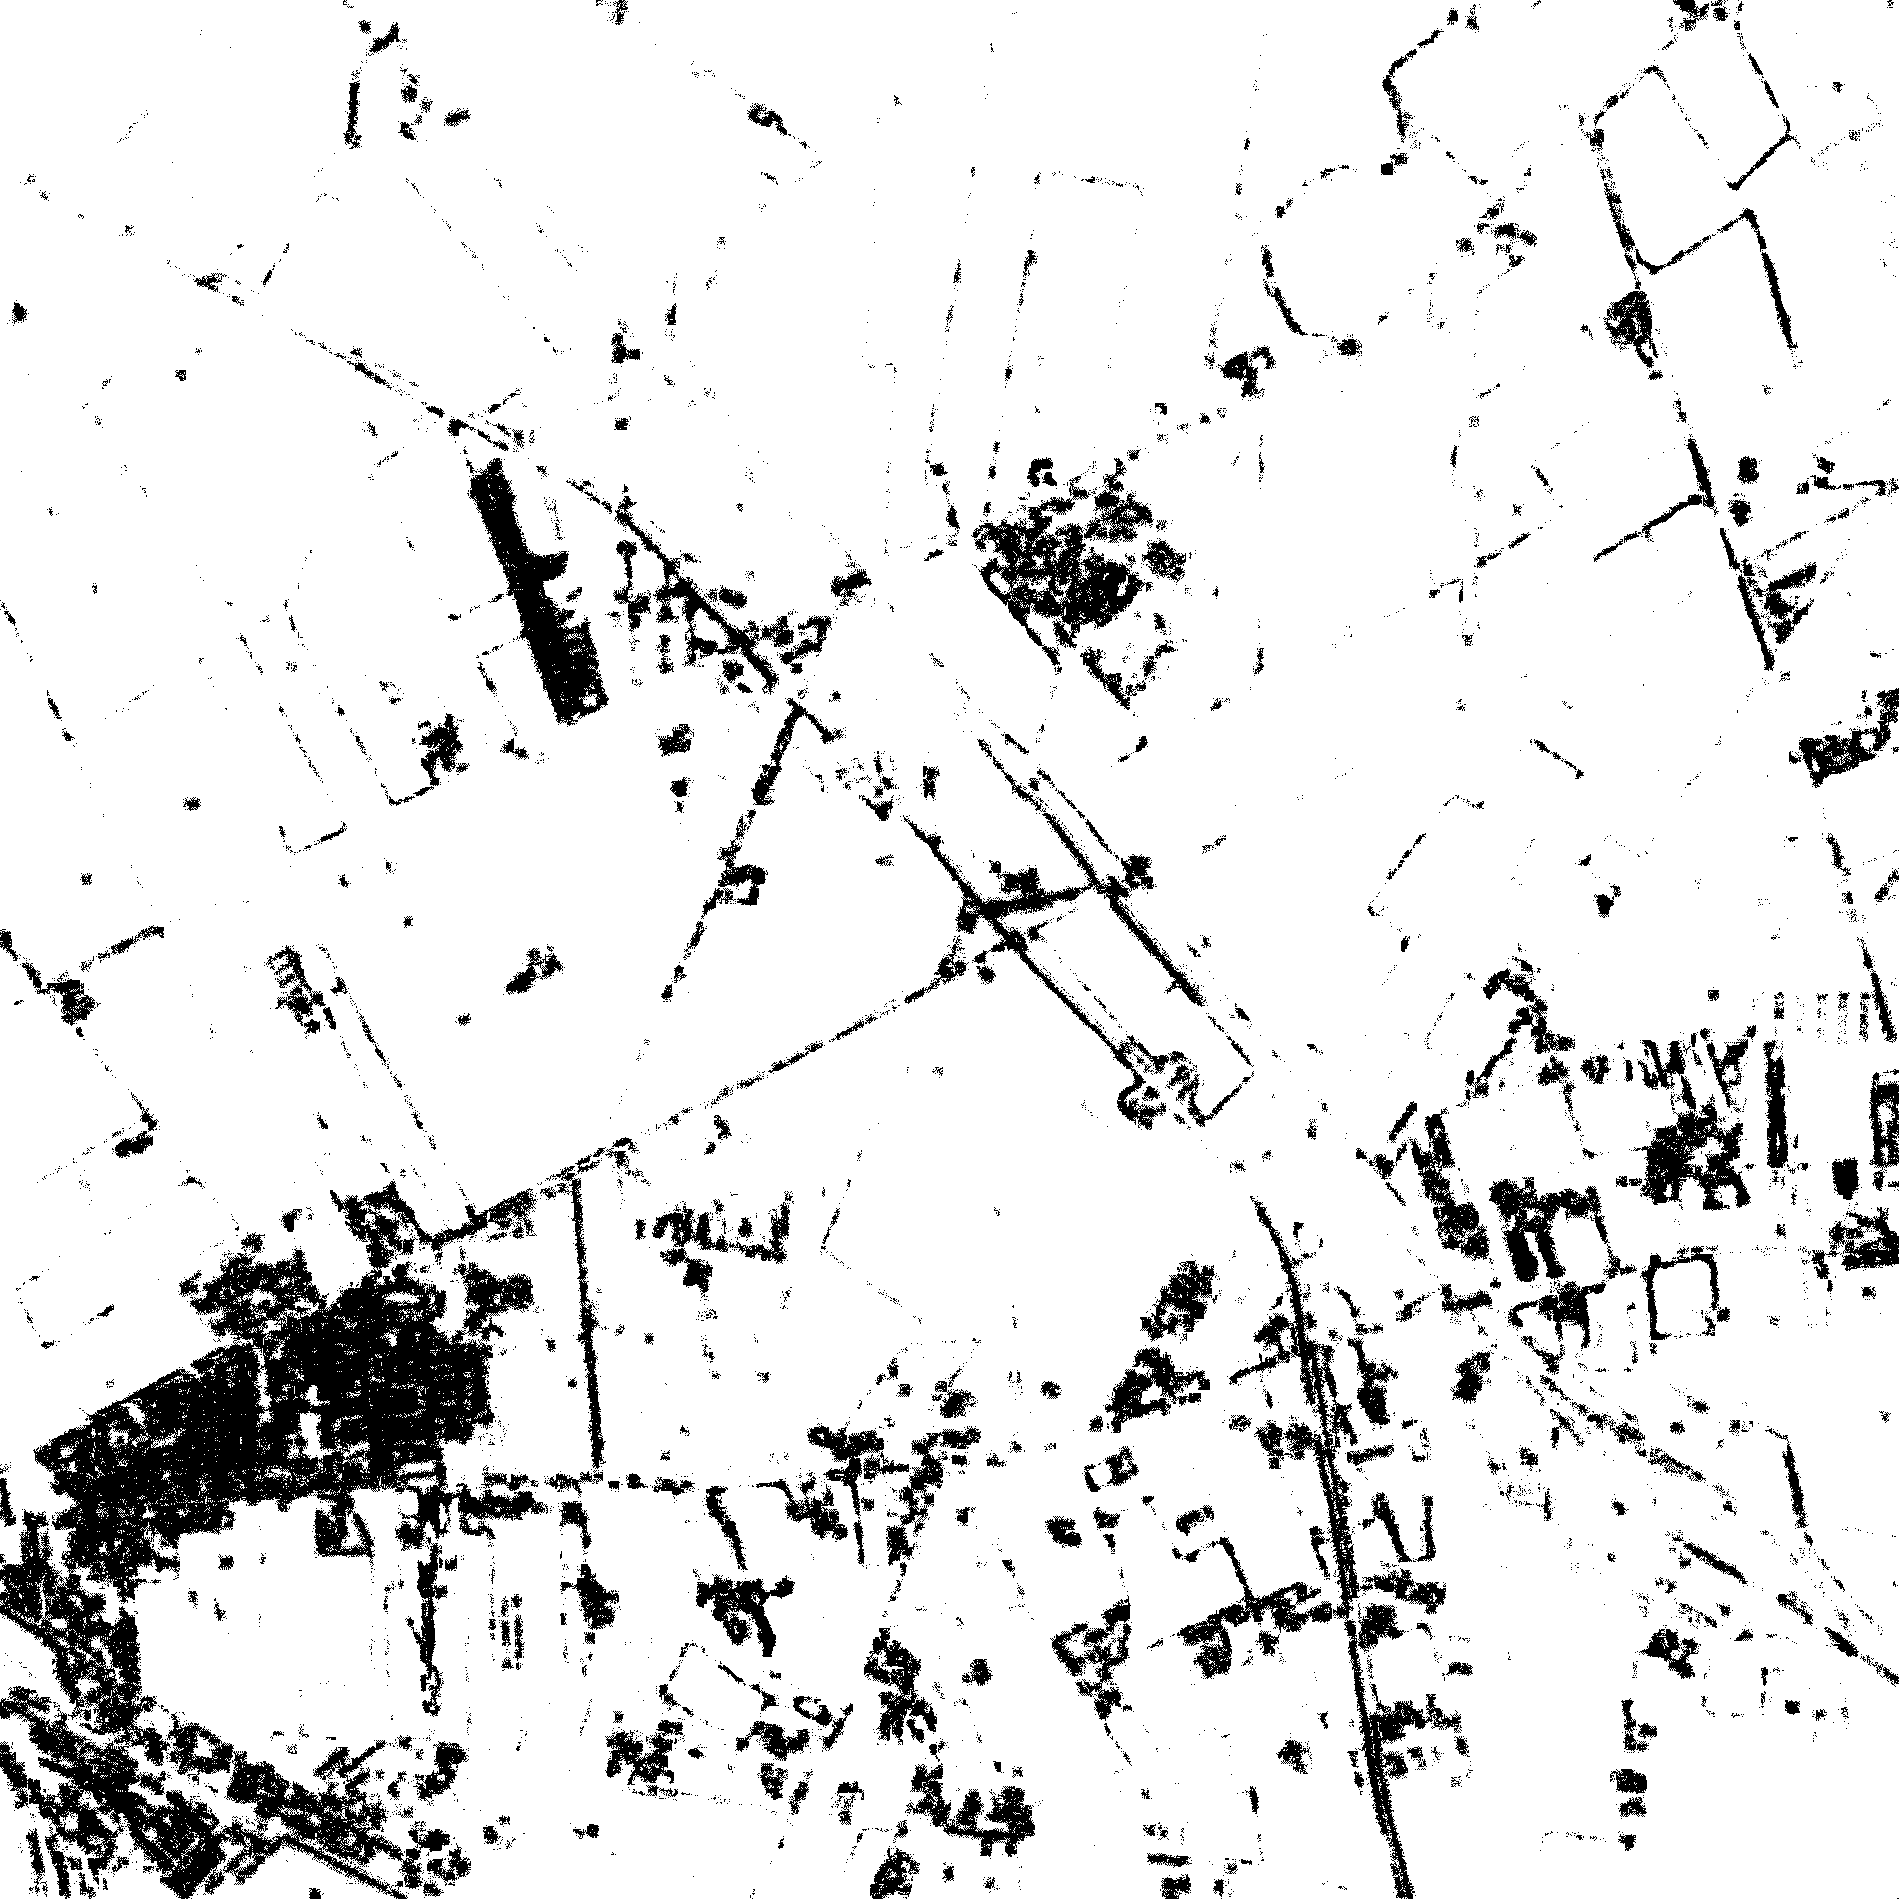
\includegraphics[width=\linewidth]{./Figures/H_005_foggia_eta4.png}
\caption{Binary map ($\eta=4$)}
\label{fig:fogc5}
\end{subfigure}

\caption{Detection of heterogeneous areas in a SAR image over Foggia. (a) $p$-value map with a fixed $7\times7$ window. (b–e) $p$-value maps with adaptive windows ($W_{\min}=5$, $W_{\max}=11$) for $\eta=1$--$4$. (f–j) Binary decision maps at $0.05$ significance level.}
\label{fig:foggia}
\end{figure*}

In the \(p\)-value maps, dark-red tones (\(p \approx 0\)) concentrate on
heterogeneous areas such as urban blocks, harbor structures, and field
boundaries, while blue tones (\(p \approx 1\)) dominate open water and
uniform surfaces. Intermediate values reveal transitional textures,
where the adaptive approach provides cleaner and more stable estimates
in homogeneous regions, while preserving finer edges in heterogeneous
regions. The binary maps make the separation between homogeneous and
textured areas explicit, showing that the adaptive strategy preserves
fine details that are partially lost with the fixed window.

The effect of the smoothing parameter \(\eta\) is particularly evident
in the San Francisco scene \((L = 4)\) in Figure~\ref{fig:sanfrancisco},
where speckle is strongest. The adaptive map with \(\eta = 2\) provides
the clearest separation between urban blocks, water, and intermediate
textured areas. For larger values, such as \(\eta = 3\) and
\(\eta = 4\), the maps become increasingly saturated in red because the
window grows more often and tends to mix classes within the local
window. This produces thicker building fronts and more detections in
moderately textured zones, but with a visible loss of spatial precision.

As \(L\) increases \DIFdelbegin \DIFdel{(}\DIFdelend \DIFaddbegin \DIFadd{in the }\DIFaddend Munich, Dublin, \DIFdelbegin \DIFdel{Foggia)}\DIFdelend \DIFaddbegin \DIFadd{and Foggia scenes}\DIFaddend , speckle
decreases and the \DIFdelbegin \DIFdel{overall performance improves, yet }\DIFdelend \DIFaddbegin \DIFadd{resulting maps become visually cleaner. Even under
these lower-speckle conditions, }\DIFaddend the adaptive scheme still provides
visible advantages: homogeneous areas become smoother\DIFaddbegin \DIFadd{, }\DIFaddend while fine
structures such as roads and field boundaries \DIFdelbegin \DIFdel{remain visible}\DIFdelend \DIFaddbegin \DIFadd{are better preserved}\DIFaddend .
Visual inspection suggests that \(\eta\) values between \(2\) and \(3\)
provide the most balanced results. With \(\eta = 1\), the outcome is
close to the fixed-window case, offering little improvement, whereas
\(\eta = 4\) tends to oversmooth the images, causing blurred edges and
loss of fine details (see panels (j) in
Figures~\ref{fig:munich}-\DIFdelbegin \DIFdel{-}\DIFdelend  \ref{fig:foggia}).

These findings highlight the advantages of the adaptive approach, which
better preserves heterogeneous features while enhancing the clarity of
homogeneous areas, consistent with the behavior observed in the
simulated experiment.

This agreement confirms that moderate values of \(\eta\) offer the best
compromise between window growth and spatial resolution, avoiding the
excessive smoothing produced by larger thresholds.

In addition to the visual analysis presented, we measured execution
times to assess the computational cost of the proposed method.
Table~\ref{tbl-exec-times} reports the processing times for the Tsallis
entropy-based test using fixed \(7\times7\) windows and, for comparison,
the adaptive variant with window sizes ranging from \(5\times5\) to
\(11\times11\) for \(\eta=1\), \(2\), \(3\), and \(4\). Times are
reported in minutes and seconds (mm:ss).

\renewcommand{\arraystretch}{1.4}

\begin{table}[hbt]

\caption{\label{tbl-exec-times}Execution times for heterogeneity
detection using fixed and adaptive windows \DIFaddbeginFL \DIFaddFL{in minutes and seconds}\DIFaddendFL .}

\centering{

\centering\begingroup\fontsize{24}{26}\selectfont

\resizebox{\ifdim\width>\linewidth\linewidth\else\width\fi}{!}{
\begin{tabular}{>{\centering\arraybackslash}p{5.5cm}>{\centering\arraybackslash}p{3cm}>{\centering\arraybackslash}p{3cm}>{\centering\arraybackslash}p{3cm}>{\centering\arraybackslash}p{3cm}>{\centering\arraybackslash}p{3cm}}
\toprule
\multicolumn{1}{c}{\textbf{Scene}} & \multicolumn{1}{c}{ $7\times7$} & \multicolumn{1}{c}{ $\eta=1$} & \multicolumn{1}{c}{ $\eta=2$} & \multicolumn{1}{c}{ $\eta=3$} & \multicolumn{1}{c}{ $\eta=4$}\\
\midrule
Simulated & 03:23 & 03:20 & 03:36 & 03:44 & 03:49\\
San Francisco & 10:58 & 11:26 & 13:37 & 14:11 & 14:27\\
Munich & 07:02 & 8:54 & 10:52 & 11:29 & 11:45\\
Dublin & 14:31 & 15:22 & 16:14 & 16:24 & 16:43\\
Foggia & 21:01 & 23:10 & 26:07 & 26:22 & 26:55\\
\bottomrule
\end{tabular}}
\endgroup{}

}

\end{table}%

Overall, the fixed-window Tsallis approach is the fastest across all
scenes, whereas the adaptive version requires longer processing times
due to the per-pixel window-size selection (border-statistics and
thresholding) and the frequent use of larger windows.

The total runtime also depends on the number of bootstrap replications,
since each replication recomputes the test statistic to obtain a more
stable estimate of the Tsallis entropy measure. In our simulations, we
used \(B=100\), which provides stable and reliable estimates with
moderate computational cost (the running time increases by, at most, a
factor of \(15\)). Stable results can already be achieved with
\(B\geq50\), whereas larger values yield smoother \(p\)-value
distributions at the expense of longer processing times.

\subsection{Quantitative Evaluation}\label{quantitative-evaluation}

To quantitatively assess detection performance, regions of interest
(ROIs) were defined to establish a ground reference for both the
simulated and actual SAR scenes. In the simulated image, two rectangular
ROIs were defined: a heterogeneous region (red, class 1) and a
homogeneous region (blue, class 0). For the four real SAR datasets (San
Francisco, Munich, Dublin, and Foggia), eight polygonal ROIs were
selected per scene (four per class), also labeled as class 1 for
heterogeneous and class 0 for homogeneous, as shown in
Figure~\ref{fig:image_roi}. All polygons were rasterized to the spatial
grid of each SAR image, producing a consistent binary reference mask
used for evaluation.

\begin{figure*}[hbt]
    \centering
        \begin{subfigure}{0.165\textwidth}
        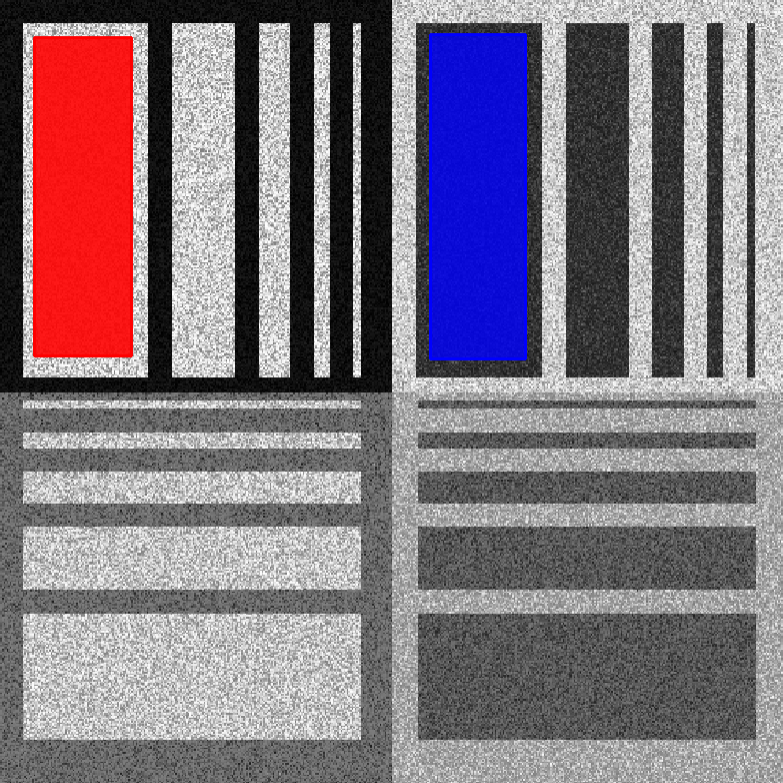
\includegraphics[width=\linewidth]{./Figures/Rois_simulated2.png}
        \caption{Simulated image}
        \label{fig:roi1}
    \end{subfigure}
    \hspace{0.00001\textwidth}
  \begin{subfigure}{0.165\textwidth}
        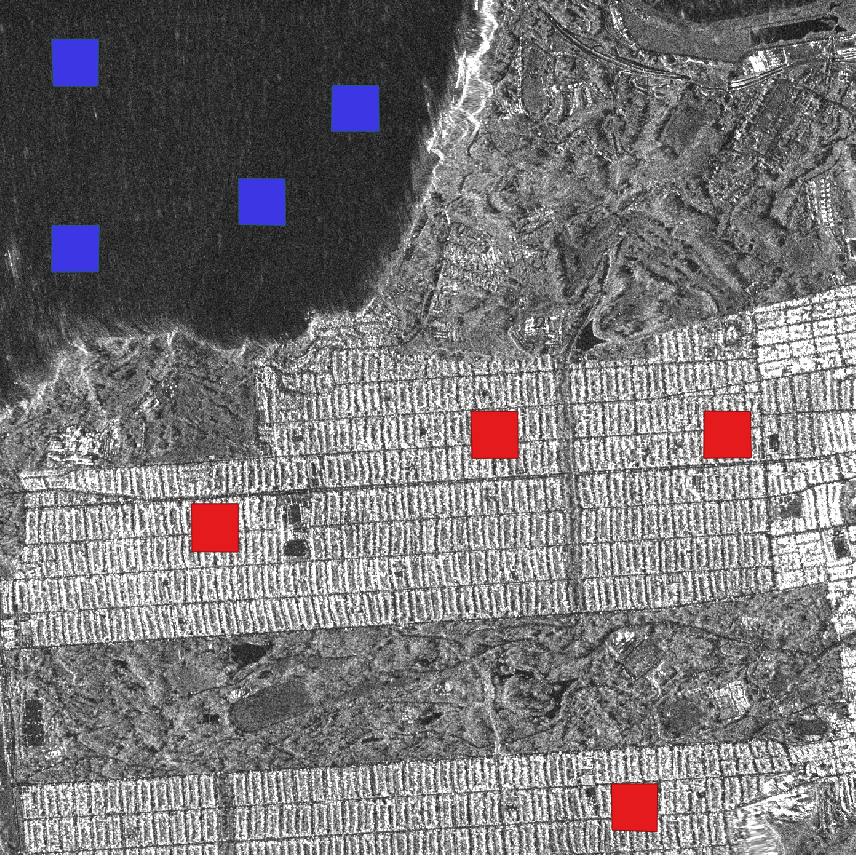
\includegraphics[width=\linewidth]{./Figures/Rois_Sanfrancisco.png}
        \caption{San Francisco }
        \label{fig:roi2}
    \end{subfigure}
    \hspace{0.00001\textwidth}
    \begin{subfigure}{0.164\textwidth}
        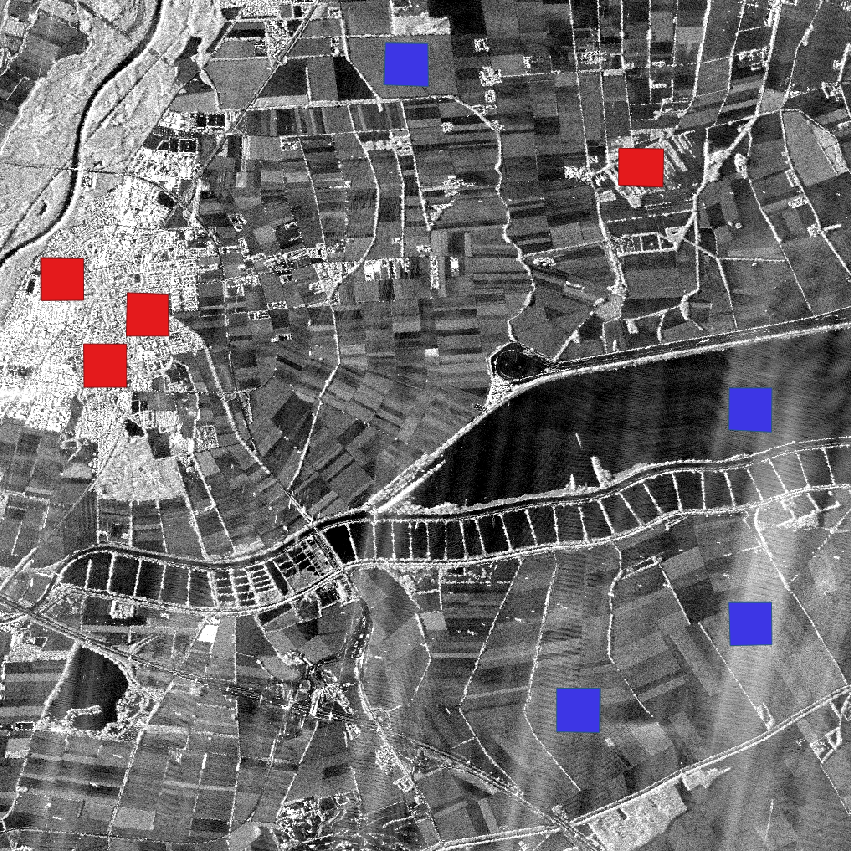
\includegraphics[width=\linewidth]{./Figures/Rois_Munich.png}
        \caption{Munich }
        \label{fig:roi3}
    \end{subfigure}
    \hspace{0.00001\textwidth}
    \begin{subfigure}{0.165\textwidth}
        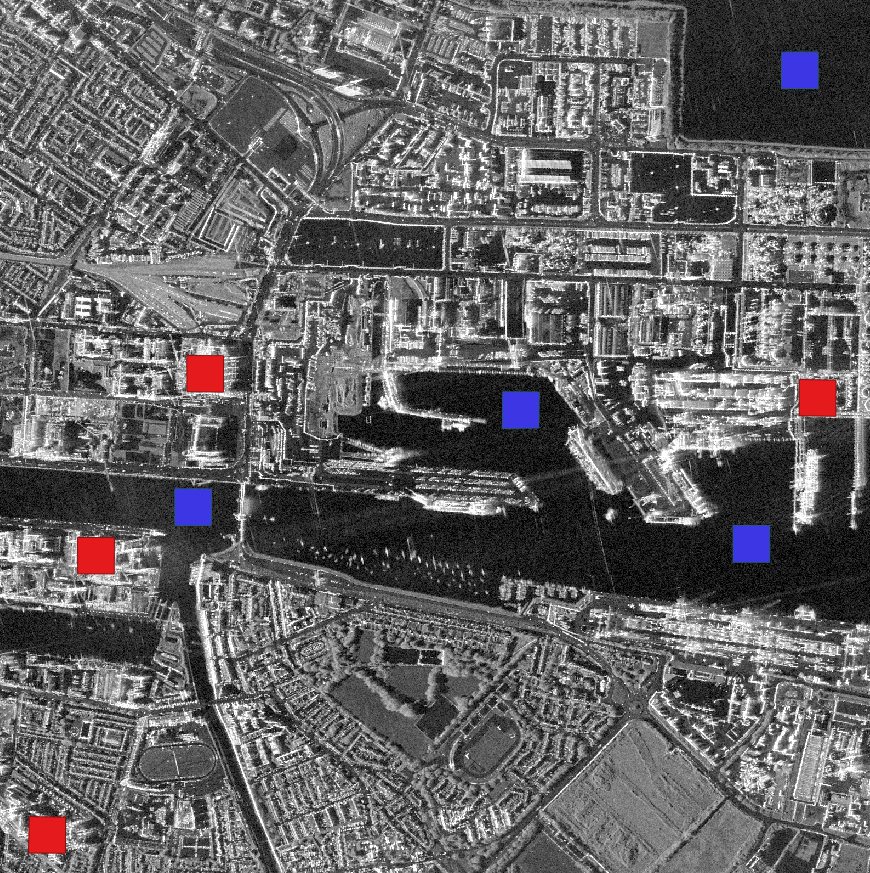
\includegraphics[width=\linewidth]{./Figures/Rois_Dublin.png}
        \caption{Dublin }
        \label{fig:roi4}
    \end{subfigure}
    \hspace{0.00001\textwidth}
    \begin{subfigure}{0.165\textwidth}
        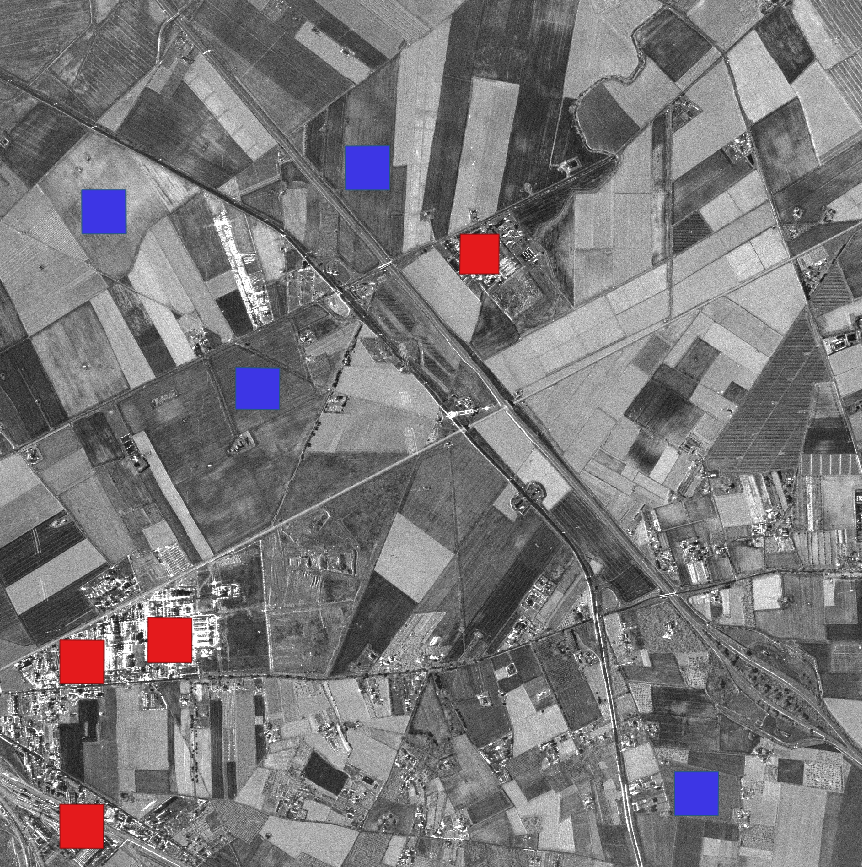
\includegraphics[width=\linewidth]{./Figures/Rois_Foggia.png}
        \caption{Foggia }
        \label{fig:roi5}
    \end{subfigure}
    \caption{Selected ROIs for the quantitative evaluation. Red polygons indicate
heterogeneous areas (class 1), and blue polygons indicate homogeneous areas (class 0).}
    \label{fig:image_roi}
\end{figure*}

We thresholded the \(p\)-value maps at \(0.05\), labeling each pixel as
heterogeneous (1) or homogeneous (0), and compared these decision maps
with the ground truth to compute the F1-score (\(F_1\)), Kappa
coefficient (\(\kappa\)), and overall accuracy (OA). The quantitative
evaluation considered the fixed \(7 \times 7\) sliding window and the
adaptive window controlled by the parameter \(\eta\). The results are
shown in Table~\ref{tbl-metrics-tsallis2}.

\renewcommand{\arraystretch}{1.1}

\begin{table}[hbt]

\caption{\label{tbl-metrics-tsallis2}Quantitative measures of
heterogeneity detection.}

\centering{

\centering\begingroup\fontsize{9}{11}\selectfont

\resizebox{\ifdim\width>\linewidth\linewidth\else\width\fi}{!}{
\begin{tabular}{lcccc}
\toprule
\multicolumn{1}{c}{\textbf{Scene}} & \multicolumn{1}{c}{\textbf{Test} $S_{\widetilde{T}_{\lambda}}$} & \multicolumn{1}{c}{$\bm{F_1}$} & \multicolumn{1}{c}{$\kappa$} & \multicolumn{1}{c}{\textbf{OA}}\\
\midrule
 & Fixed $7\times7$ & $0.980$ & $0.960$ & $0.980$\\

 & Adapt. $\eta=1$ & $0.960$ & $0.923$ & $0.961$\\

 & Adapt. $\eta=2$ & $0.969$ & $0.940$ & $0.970$\\

 & Adapt. $\eta=3$ & \bm{$0.983$} & \bm{$0.966$} & \bm{$0.983$}\\

\multirow{-5}{*}{\raggedright\arraybackslash Simulated} & Adapt. $\eta=4$ & $0.976$ & $0.953$ & $0.976$\\
\cmidrule{1-5}
 & Fixed $7\times7$ & $0.775$ & $0.638$ & $0.820$\\

 & Adapt. $\eta=1$ & $0.810$ & $0.686$ & $0.844$\\

 & Adapt. $\eta=2$ & \bm{$0.860$} & \bm{$0.758$} & \bm{$0.880$}\\

 & Adapt. $\eta=3$ & $0.841$ & $0.729$ & $0.866$\\

\multirow{-5}{*}{\raggedright\arraybackslash San Francisco} & Adapt. $\eta=4$ & $0.788$ & $0.655$ & $0.829$\\
\cmidrule{1-5}
 & Fixed $7\times7$ & $0.899$ & $0.820$ & $0.911$\\

 & Adapt. $\eta=1$ & $0.850$ & $0.744$ & $0.873$\\

 & Adapt. $\eta=2$ & $0.901$ & $0.823$ & $0.912$\\

 & Adapt. $\eta=3$ & \bm{$0.935$} & \bm{$0.880$} & \bm{$0.940$}\\

\multirow{-5}{*}{\raggedright\arraybackslash Munich} & Adapt. $\eta=4$ & $0.914$ & $0.845$ & $0.923$\\
\cmidrule{1-5}
 & Fixed $7\times7$ & $0.880$ & $0.812$ & $0.912$\\

 & Adapt. $\eta=1$ & $0.845$ & $0.762$ & $0.890$\\

 & Adapt. $\eta=2$ & $0.883$ & $0.816$ & $0.914$\\

 & Adapt. $\eta=3$ & \bm{$0.901$} & \bm{$0.844$} & \bm{$0.926$}\\

\multirow{-5}{*}{\raggedright\arraybackslash Dublin} & Adapt. $\eta=4$ & $0.888$ & $0.823$ & $0.917$\\
\cmidrule{1-5}
 & Fixed $7\times7$ & $0.933$ & $0.876$ & $0.938$\\

 & Adapt. $\eta=1$ & $0.910$ & $0.837$ & $0.919$\\

 & Adapt. $\eta=2$ & $0.943$ & $0.892$ & $0.946$\\

 & Adapt. $\eta=3$ & \bm{$0.951$} & \bm{$0.907$} & \bm{$0.953$}\\

\multirow{-5}{*}{\raggedright\arraybackslash Foggia} & Adapt. $\eta=4$ & $0.906$ & $0.830$ & $0.915$\\
\bottomrule
\end{tabular}}
\endgroup{}

}

\end{table}%

The quantitative evaluation corroborates the visual analysis. In the
simulated image, the adaptive configuration with \(\eta = 3\) achieved
the best performance (\(F_1 = 0.983\), \(\kappa = 0.966\), OA
\(= 0.983\)), confirming its ability to clearly separate the two classes
under ideal conditions.

For the San Francisco scene (\(L = 4\)), the best performance was
obtained with \(\eta = 2\) (\(F_1 = 0.860\), \(\kappa = 0.758\), OA
\(= 0.880\)), which provided a good balance between noise suppression
and texture sensitivity in strongly speckled conditions. This matches
the visual inspection: \(\eta = 2\) provides the cleanest delineation
between built-up areas and textureless regions.

For the scenes with higher numbers of looks, Munich (\(L = 12\)), Dublin
(\(L = 16\)), and Foggia (\(L = 24\)), the best results were obtained
with \(\eta = 3\). In these images, the reduced speckle allows slightly
larger adaptive windows to stabilize the entropy estimates without
oversmoothing, which explains the advantage of \(\eta = 3\).

Across all scenes, the configuration \(\eta = 4\) presents lower
performance. This degradation is consistent with the visual effects
observed earlier: the window expands too easily, mixing textures within
\(w_{ij}\), which reduces class separability and blurs fine structures.
Although \(\eta = 4\) sometimes increases detection in heterogeneous
regions, this comes at the cost of reduced \(F_1\), lower \(\kappa\),
and more false positives, particularly around transitions.

Regarding the decision threshold, a significance level of \(0.05\) was
adopted for the binary classification of the \(p\)-value maps. This
choice provides a practical balance between false-alarm control and
sensitivity to weak texture variations. Experiments with alternative
levels confirmed the expected trade-offs: a stricter threshold
(\(0.01\)) reduces false alarms but may miss subtle features, whereas a
more relaxed one (\(0.10\)) increases sensitivity at the cost of more
false positives, particularly in highly speckled regions.

\subsection{Comparative Benchmark Between Entropy-Based
Tests}\label{sec:entropy-benchmark}

To compare the proposed Tsallis-based test with earlier entropy-based
methods for SAR imagery, we carried out a \DIFdelbegin \DIFdel{benchmark against }\DIFdelend \DIFaddbegin \DIFadd{comparison with }\DIFaddend the Shannon
and Rényi-based tests. In particular, the Shannon-based test
in~\citeproc{ref-Frery2024}{{[}22{]}} and the Rényi-based test
in~\citeproc{ref-Alpala2025}{{[}23{]}} follow the same general approach
to hypothesis testing, i.e., comparing a nonparametric entropy estimate
with its theoretical value under the \(\Gamma_{\mathrm{SAR}}\) model.

The present proposal extends that line by using the Tsallis entropy,
whose parameter \(\lambda\) provides additional flexibility to capture
departures from homogeneity in heavy-tailed and highly textured SAR
data.

This comparison is relevant because the gain of the proposed method may
come from three components: the entropy functional, the bootstrap
correction, and the adaptive window-selection strategy. To separate
these effects, we compared Shannon, Rényi, and Tsallis under the same
protocol, considering fixed and adaptive windows, with and without
bootstrap correction. The fixed window size was \(7\times7\), and the
adaptive range was \(5\times5\) to \(11\times11\).

For the adaptive configurations in this benchmark, we used the
\DIFdelbegin \DIFdel{refined
calibration }\DIFdelend \DIFaddbegin \DIFadd{standardization }\DIFaddend introduced in~\eqref{eq:standar}, which preserves the
window-dependent \DIFdelbegin \DIFdel{null centering while avoiding distortions that may
arise when a purely null-based scale is used in real scenes}\DIFdelend \DIFaddbegin \DIFadd{centering under \(\mathcal H_0\) while using an
observed scale computed from the image under analysis. This procedure
was applied separately to each entropy-based test, using the
corresponding test-statistic values and the observed scale
\(\sigma_{\mathrm{obs}}\) for that method. The comparative benchmark was
performed on the Dublin scene under a common setting for the Shannon,
Rényi, and Tsallis tests, with \(L=16\), \(\eta=3\), and adaptive
windows from \(5\times5\) to \(11\times11\). This scene is suitable for
the comparison because it provides a clear contrast between homogeneous
water areas and heterogeneous urban and harbor structures}\DIFaddend . In the Dublin
scene, this \DIFdelbegin \DIFdel{refinement produced only minor quantitative changes
and left }\DIFdelend \DIFaddbegin \DIFadd{observed-scale standardization slightly improved the
quantitative metrics while leaving }\DIFaddend the substantive conclusions
unchanged.

For the single-threshold summaries, we report \(F_1\), \(\kappa\), and
OA at the nominal decision level \(p=0.05\), since the binary decision
maps in the paper are obtained from the rule \(p_{ij}<0.05\). To verify
that the conclusions are not driven by this single choice, we also
performed a threshold sweep over \(p\)-thresholds from \(0.01\) to
\(0.20\). In contrast, the ROC curve and its area under the curve (AUC)
are threshold-free, as they are computed from the continuous score map
rather than from a single decision threshold.

Table~\ref{tbl-dublin-main-benchmark} reports the benchmark results. Two
consistent trends are observed. First, for all three entropies, the
adaptive strategy improves the corresponding fixed-window configuration
\DIFaddbegin \DIFadd{in the Dublin scene}\DIFaddend . Second, within both the fixed and adaptive
settings, the Tsallis-based test \DIFdelbegin \DIFdel{provides the strongest overall performance}\DIFdelend \DIFaddbegin \DIFadd{achieved the best quantitative results
in this Dublin benchmark}\DIFaddend .

\begin{table*}

\caption{\label{tbl-dublin-main-benchmark}Entropy-based benchmark on the Dublin SAR scene under fixed and adaptive window settings.}

\DIFdelbeginFL %DIFDELCMD < \centering{
%DIFDELCMD < 

%DIFDELCMD < \footnotesize
%DIFDELCMD < \centering
%DIFDELCMD < 

%DIFDELCMD < %\resizebox{0.94\textwidth}{!}{%
%DIFDELCMD < \begin{tabular}{ccccccc}
%DIFDELCMD < \toprule
%DIFDELCMD < \textbf{Entropy} & \textbf{Bootstrap} & \textbf{Window setting} & \textbf{AUC} & $\boldsymbol{F_1\,(p=0.05)}$ & \textbf{$\kappa(p=0.05)$} & \textbf{OA$(p=0.05)$} \\
%DIFDELCMD < \midrule
%DIFDELCMD < \multirow{4}{*}{Shannon}
%DIFDELCMD < & \xmark & Fixed $7\times7$   & 0.9509 & 0.4944 & 0.3660 & 0.7250 \\
%DIFDELCMD < & \xmark & Adaptive  & 0.9826 & 0.8218 & 0.7314 & 0.8761 \\
%DIFDELCMD < & \cmark & Fixed $7\times7$   & 0.9680 & 0.6598 & 0.5339 & 0.7921 \\
%DIFDELCMD < & \cmark & Adaptive  & 0.9887 & 0.8730 & 0.8023 & 0.9077 \\
%DIFDELCMD < \midrule
%DIFDELCMD < \multirow{4}{*}{Rényi}
%DIFDELCMD < & \xmark & Fixed $7\times7$   & 0.9625 & 0.6786 & 0.5549 & 0.8008 \\
%DIFDELCMD < & \xmark & Adaptive  & 0.9854 & 0.8554 & 0.7773 & 0.8965 \\
%DIFDELCMD < & \cmark & Fixed $7\times7$   & 0.9844 & 0.8752 & 0.8055 & 0.9091 \\
%DIFDELCMD < & \cmark & Adaptive & 0.9931 & 0.8941 & 0.8329 & 0.9216 \\
%DIFDELCMD < \midrule
%DIFDELCMD < \multirow{4}{*}{Tsallis}
%DIFDELCMD < & \xmark & Fixed $7\times7$   & 0.9727 & 0.7332 & 0.6188 & 0.8275 \\
%DIFDELCMD < & \xmark & Adaptive  & 0.9894 & 0.8748 & 0.8049 & 0.9089 \\
%DIFDELCMD < & \cmark & Fixed $7\times7$   & 0.9937 & 0.8812 & 0.8141 & 0.9130 \\
%DIFDELCMD < & \cmark & Adaptive  & \textbf{0.9990} & \textbf{0.9143} & \textbf{0.8630} & \textbf{0.9353} \\
%DIFDELCMD < \bottomrule
%DIFDELCMD < \end{tabular}%
%DIFDELCMD < %}
%DIFDELCMD < 

%DIFDELCMD < }
%DIFDELCMD < %%%
\DIFdelendFL \DIFaddbeginFL \centering{

\footnotesize
\centering


%\resizebox{0.94\textwidth}{!}{%
\begin{tabular}{ccccccc}
\toprule
\textbf{Entropy} 
& \textbf{Bootstrap} 
& \textbf{Window setting} 
& \textbf{AUC} 
& $\boldsymbol{F_1 \, (p=0.05)}$ 
& $\boldsymbol{\kappa \, (p=0.05)}$ 
& \textbf{OA} \, \boldsymbol{$(p=0.05)$} \\
\midrule
\multirow{4}{*}{Shannon}
& \xmark & Fixed $7\times7$   & 0.9509 & 0.4944 & 0.3660 & 0.7250 \\
& \xmark & Adaptive  & 0.9826 & 0.8218 & 0.7314 & 0.8761 \\
& \cmark & Fixed $7\times7$   & 0.9680 & 0.6598 & 0.5339 & 0.7921 \\
& \cmark & Adaptive  & 0.9887 & 0.8730 & 0.8023 & 0.9077 \\
\midrule
\multirow{4}{*}{Rényi}
& \xmark & Fixed $7\times7$   & 0.9625 & 0.6786 & 0.5549 & 0.8008 \\
& \xmark & Adaptive  & 0.9854 & 0.8554 & 0.7773 & 0.8965 \\
& \cmark & Fixed $7\times7$   & 0.9844 & 0.8752 & 0.8055 & 0.9091 \\
& \cmark & Adaptive & 0.9931 & 0.8941 & 0.8329 & 0.9216 \\
\midrule
\multirow{4}{*}{Tsallis}
& \xmark & Fixed $7\times7$   & 0.9727 & 0.7332 & 0.6188 & 0.8275 \\
& \xmark & Adaptive  & 0.9894 & 0.8748 & 0.8049 & 0.9089 \\
& \cmark & Fixed $7\times7$   & 0.9937 & 0.8812 & 0.8141 & 0.9130 \\
& \cmark & Adaptive  & \textbf{0.9990} & \textbf{0.9143} & \textbf{0.8630} & \textbf{0.9353} \\
\bottomrule
\end{tabular}%
%}

}
\DIFaddendFL 

\end{table*}%

The best configuration is the bootstrap-corrected adaptive Tsallis
method, which achieved the highest AUC, \(F_1(p=0.05)\),
\(\kappa(p=0.05)\), and OA\((p=0.05)\). These results indicate that the
improvement is not explained only by adaptive windowing, since the
Tsallis entropy itself also provides additional discriminatory power
when combined with bootstrap correction and adaptive window selection.

Figure~\ref{fig:roc_entropy_benchmark} provides a threshold-free
comparison through ROC curves. \DIFdelbegin \DIFdel{In both the fixed and adaptive settings}\DIFdelend \DIFaddbegin \DIFadd{For the Dublin scene}\DIFaddend , the Tsallis-based
method \DIFdelbegin \DIFdel{outperforms }\DIFdelend \DIFaddbegin \DIFadd{showed a more favorable AUC profile than }\DIFaddend the Shannon and
Rényi-based alternatives \DIFaddbegin \DIFadd{in both the fixed and adaptive settings}\DIFaddend , with
the \DIFdelbegin \DIFdel{largest }\DIFdelend \DIFaddbegin \DIFadd{clearest }\DIFaddend separation observed in the adaptive bootstrap-corrected
case.

\begin{figure}[hbt]
  \centering
  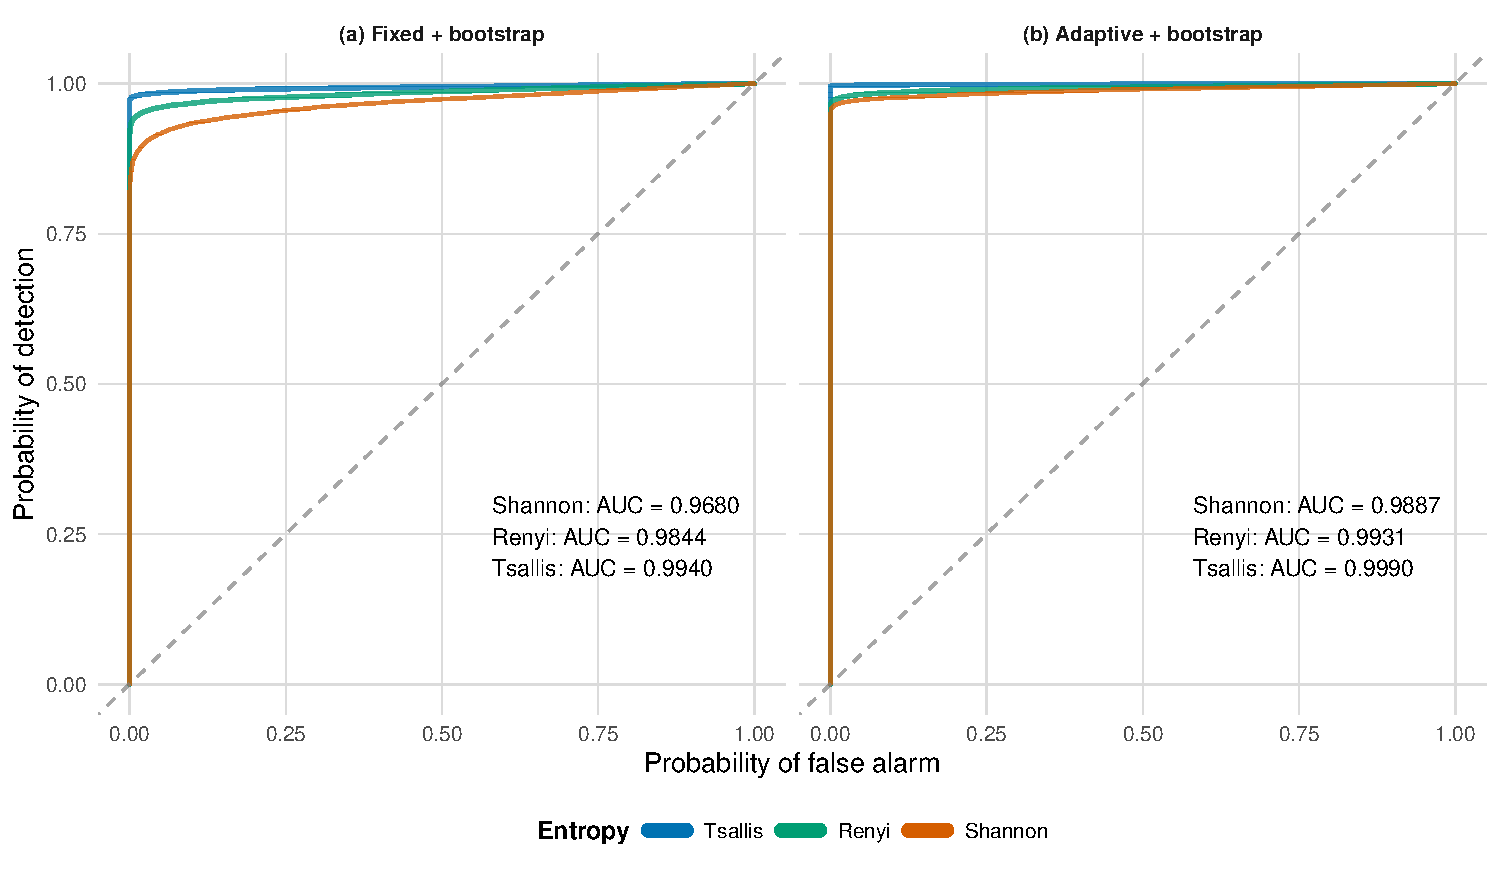
\includegraphics[width=0.99\columnwidth]{Figures-R1/dublin_entropy_benchmark_roc_2panels.pdf}
  \caption{ROC comparison on the Dublin SAR scene for Shannon, Rényi, and Tsallis under bootstrap-corrected fixed and adaptive settings.}
  \label{fig:roc_entropy_benchmark}
\end{figure}

Figure~\ref{fig:threshold_entropy_benchmark} shows the corresponding
\(F_1\) threshold sweep for \(p\)-thresholds from \(0.01\) to \(0.20\).
\DIFdelbegin \DIFdel{The same ranking is observed across thresholds, with Tsallis performing
best, }\DIFdelend \DIFaddbegin \DIFadd{For the Dublin scene, the Tsallis-based method achieved the best \(F_1\)
scores across the evaluated thresholds, }\DIFaddend followed by Rényi and Shannon.

\begin{figure}[hbt]
  \centering
  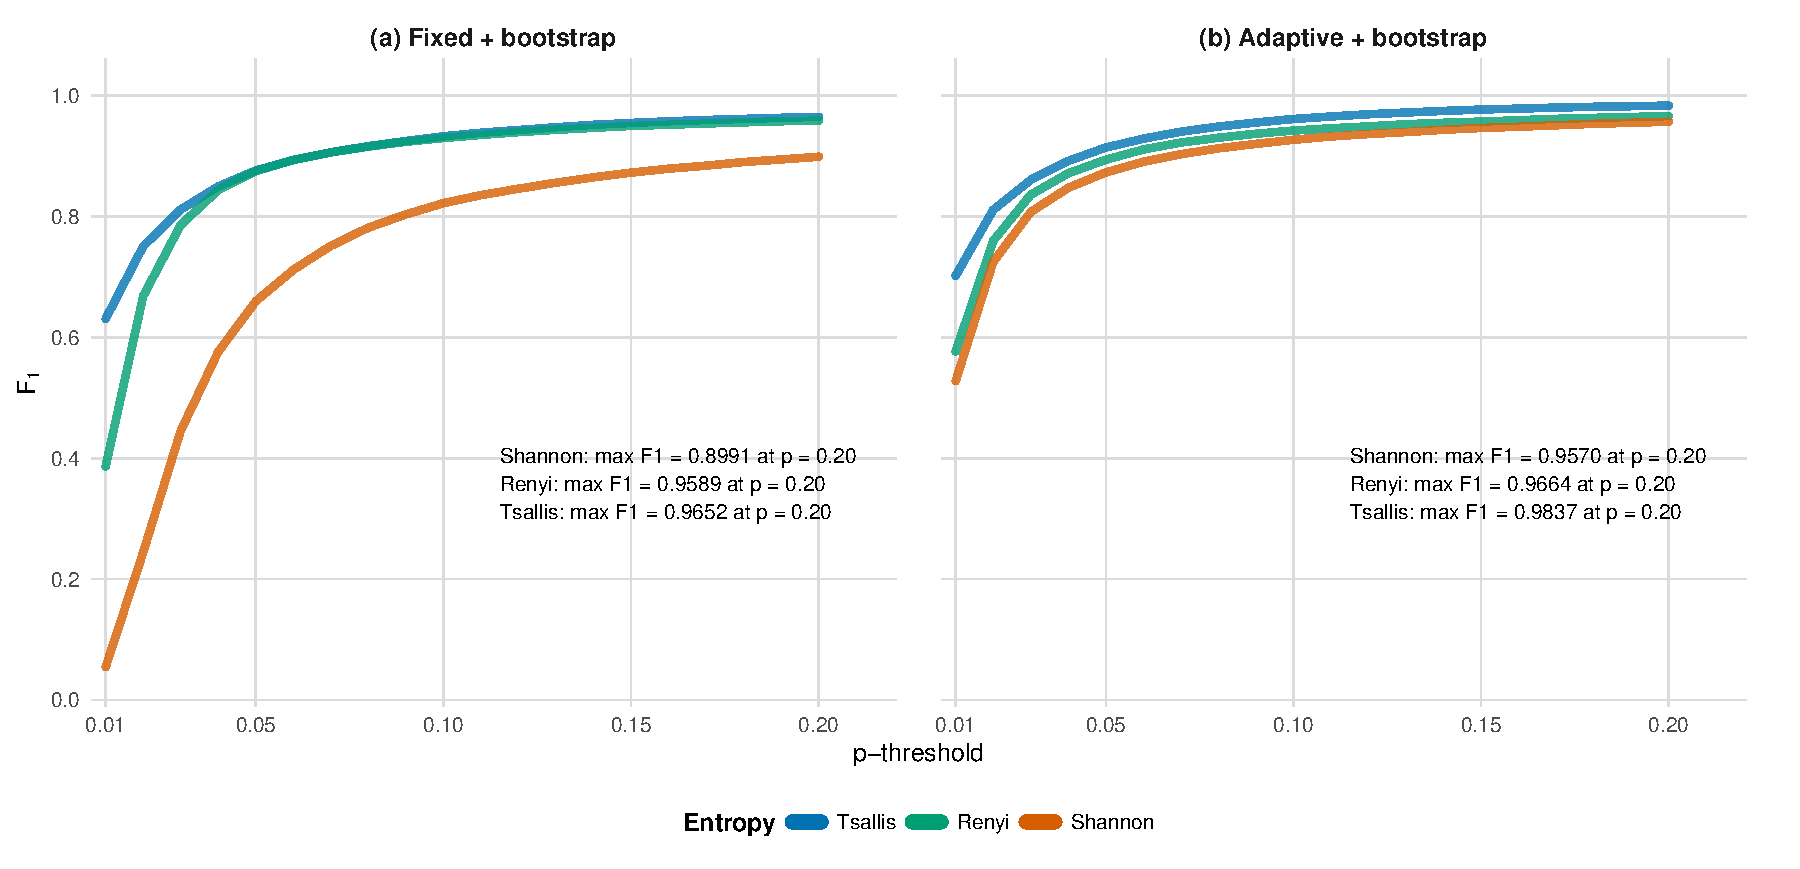
\includegraphics[width=0.99\columnwidth]{Figures-R1/dublin_benchmark_f1_threshold_two_panels.pdf}
  \caption{$F_1$ threshold sweep on the Dublin SAR scene for Shannon, Rényi, and Tsallis under bootstrap-corrected fixed and adaptive settings, using $p$-thresholds from $0.01$ to $0.20$.}
  \label{fig:threshold_entropy_benchmark}
\end{figure}

To complement the quantitative benchmark, we also performed a
qualitative comparison on the Dublin SAR scene using the
bootstrap-corrected adaptive configurations of the Shannon, Rényi, and
Tsallis entropy-based tests.
Figure~\ref{fig:dublin_qualitative_comparison} shows the corresponding
full-scene \(p\)-value maps. The three methods consistently identify the
main heterogeneous urban and harbor structures. However, the
Tsallis-based map exhibits sharper local contrast and a more coherent
delineation of heterogeneous areas, while Shannon appears comparatively
less selective and Rényi provides an intermediate behavior.

\begin{figure*}[hbt]
\centering

\begin{minipage}[t]{0.30\textwidth}
    \centering
    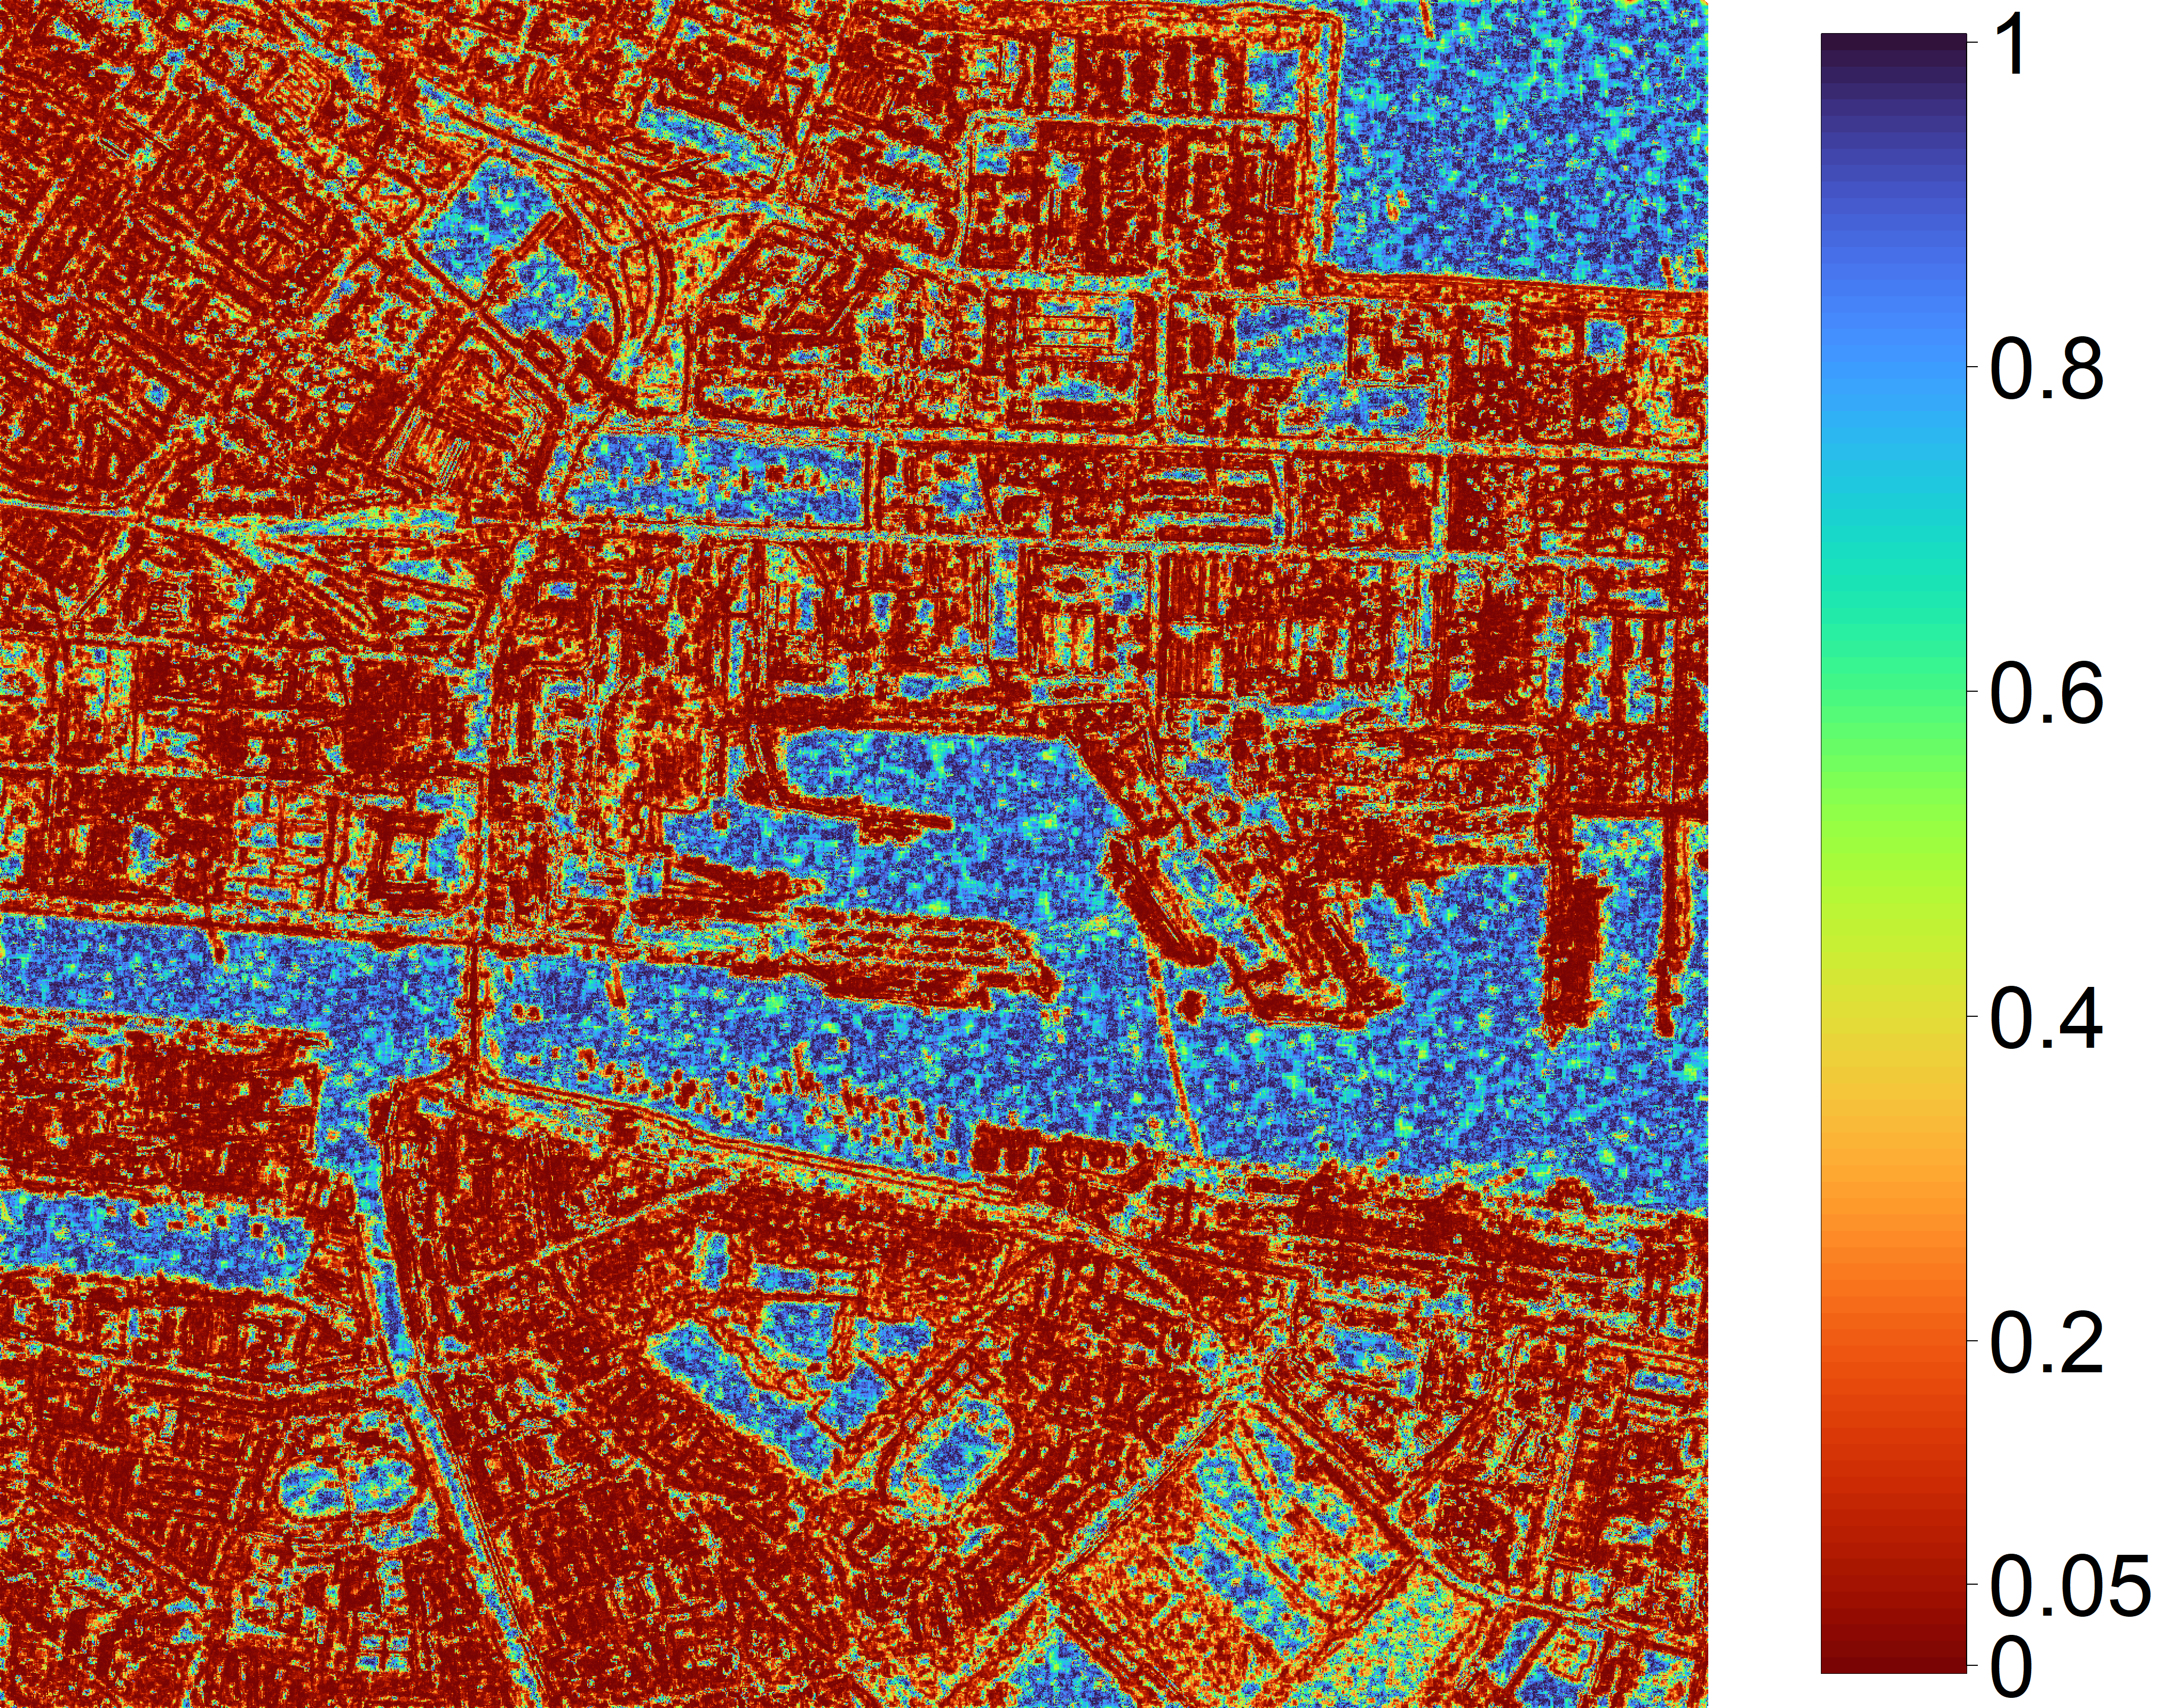
\includegraphics[width=\linewidth]{Figures-R1/dublin_shannon_adaptive.png}

    \vspace{2pt}
    \textbf{(a)}
\end{minipage}
\hfill
\begin{minipage}[t]{0.30\textwidth}
    \centering
    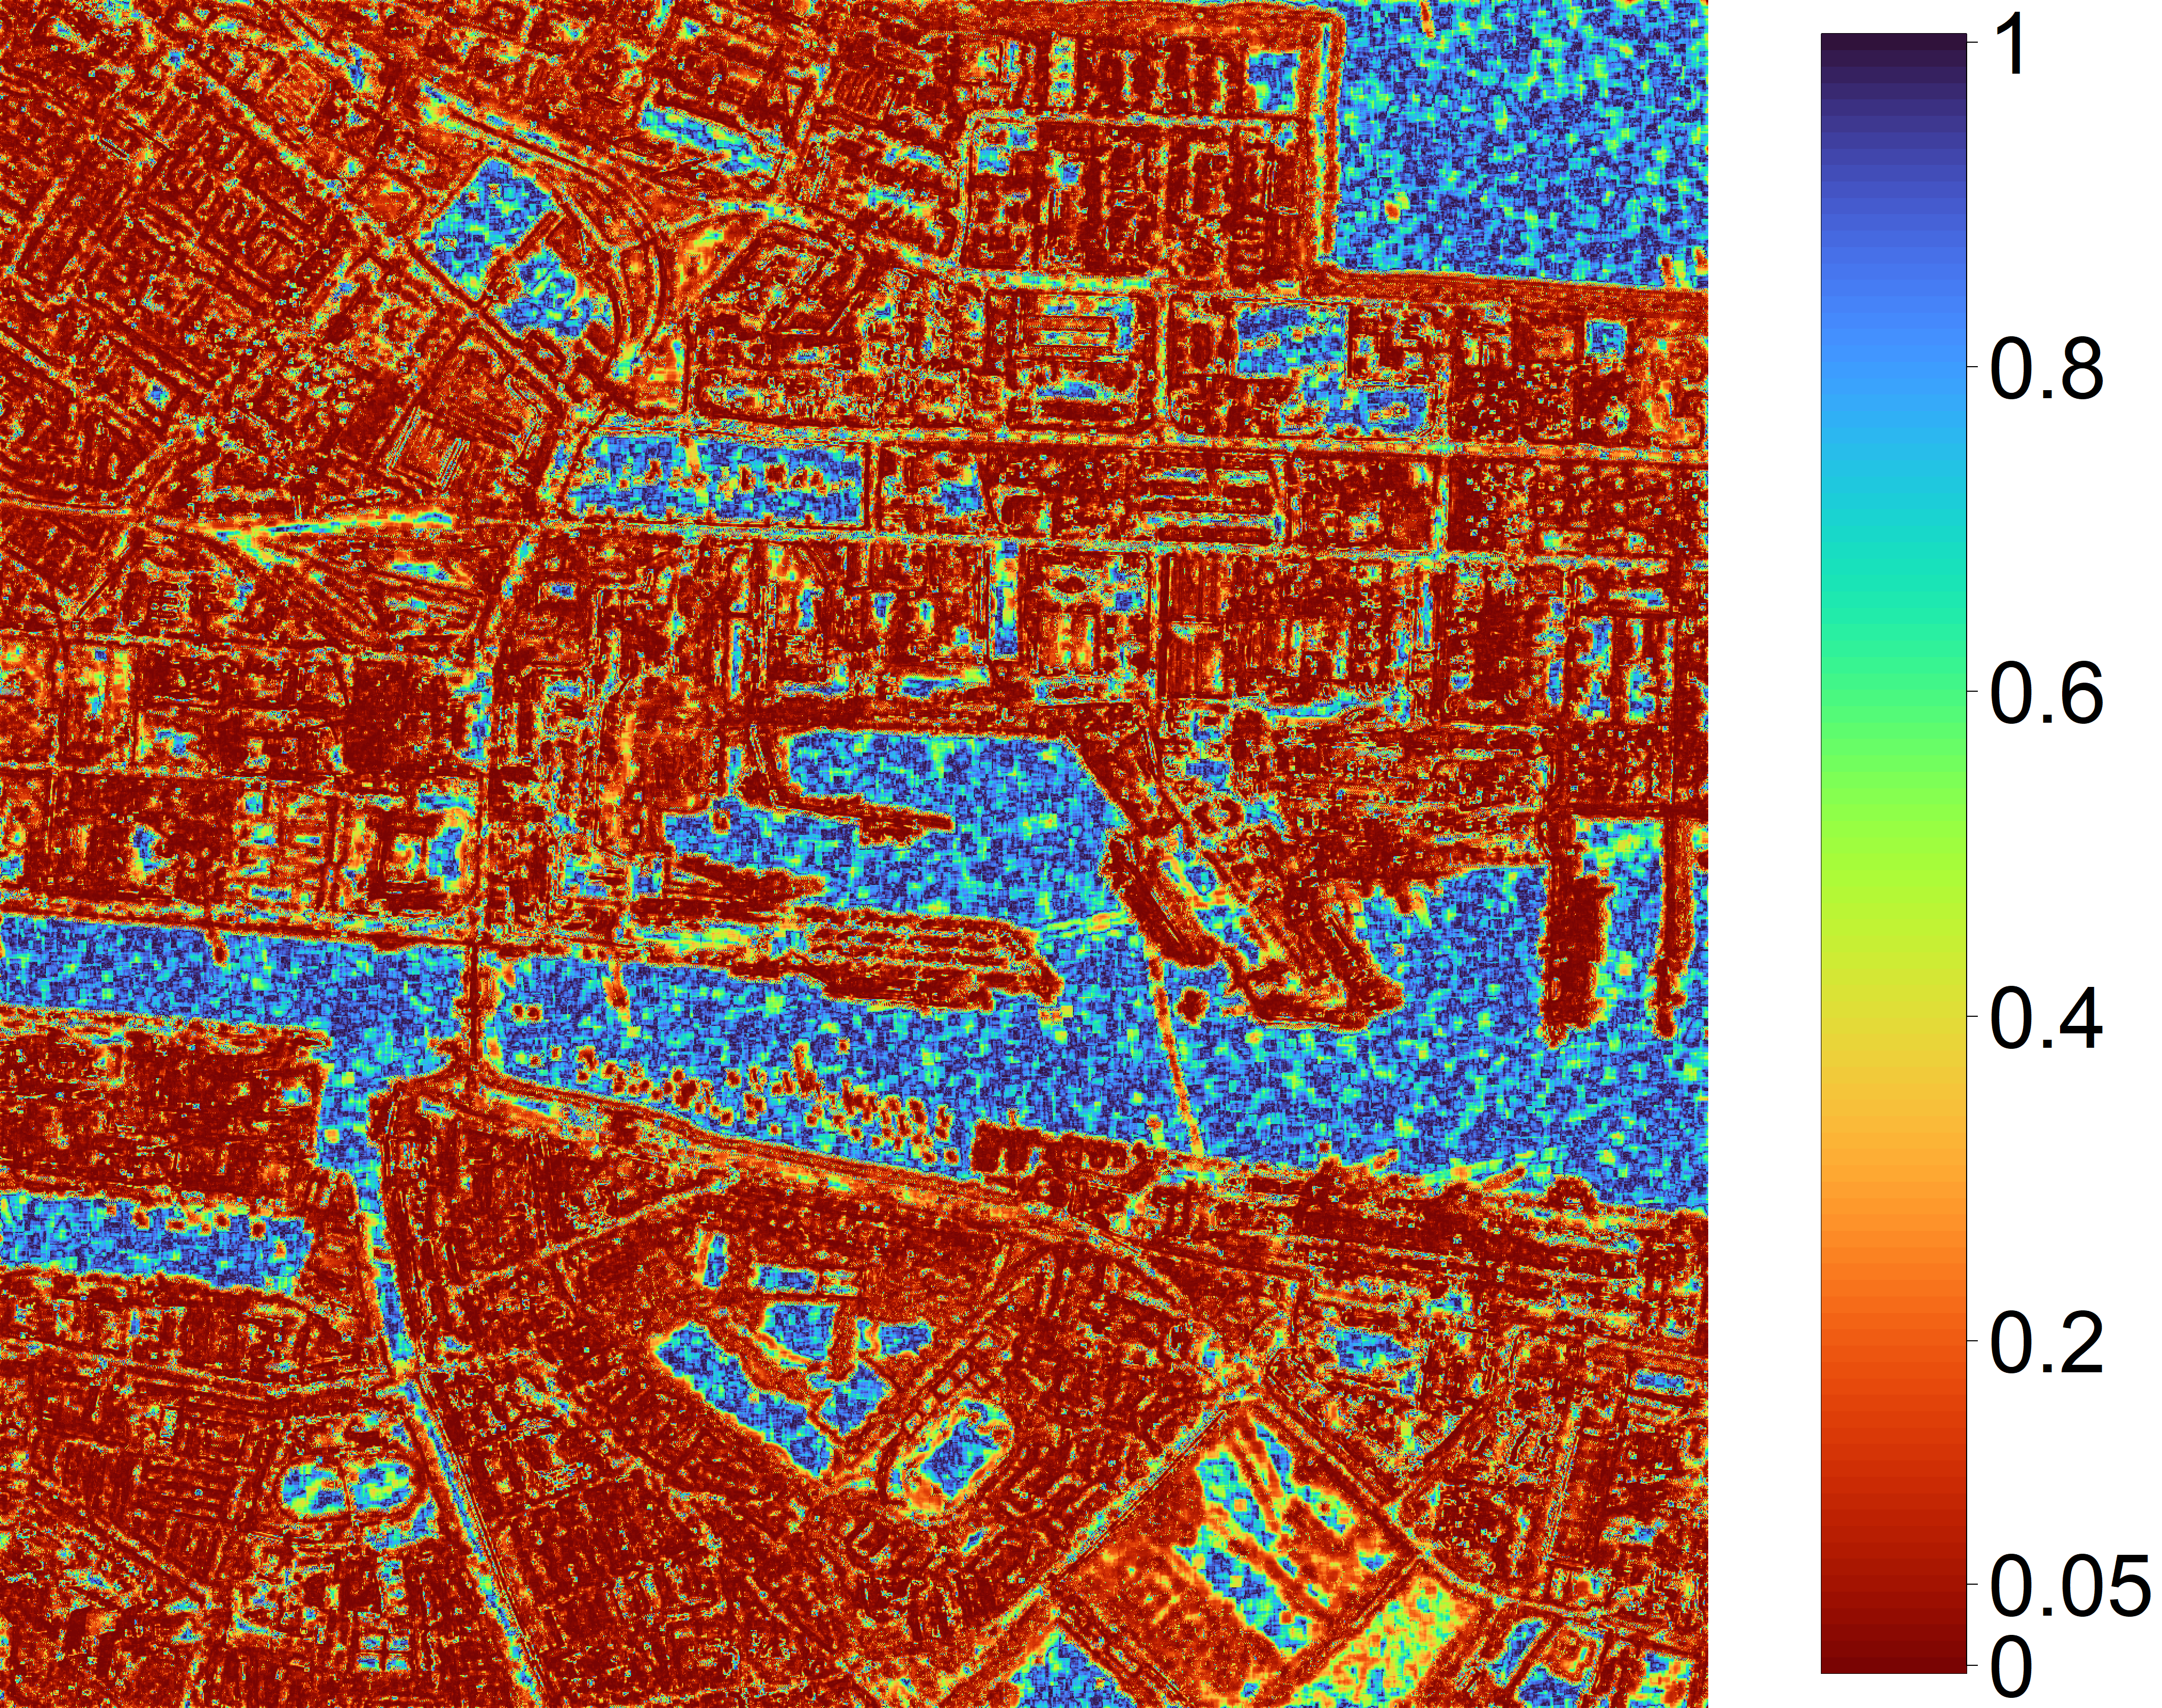
\includegraphics[width=\linewidth]{Figures-R1/dublin_renyi_adaptive.png}

    \vspace{2pt}
    \textbf{(b)}
\end{minipage}
\hfill
\begin{minipage}[t]{0.30\textwidth}
    \centering
    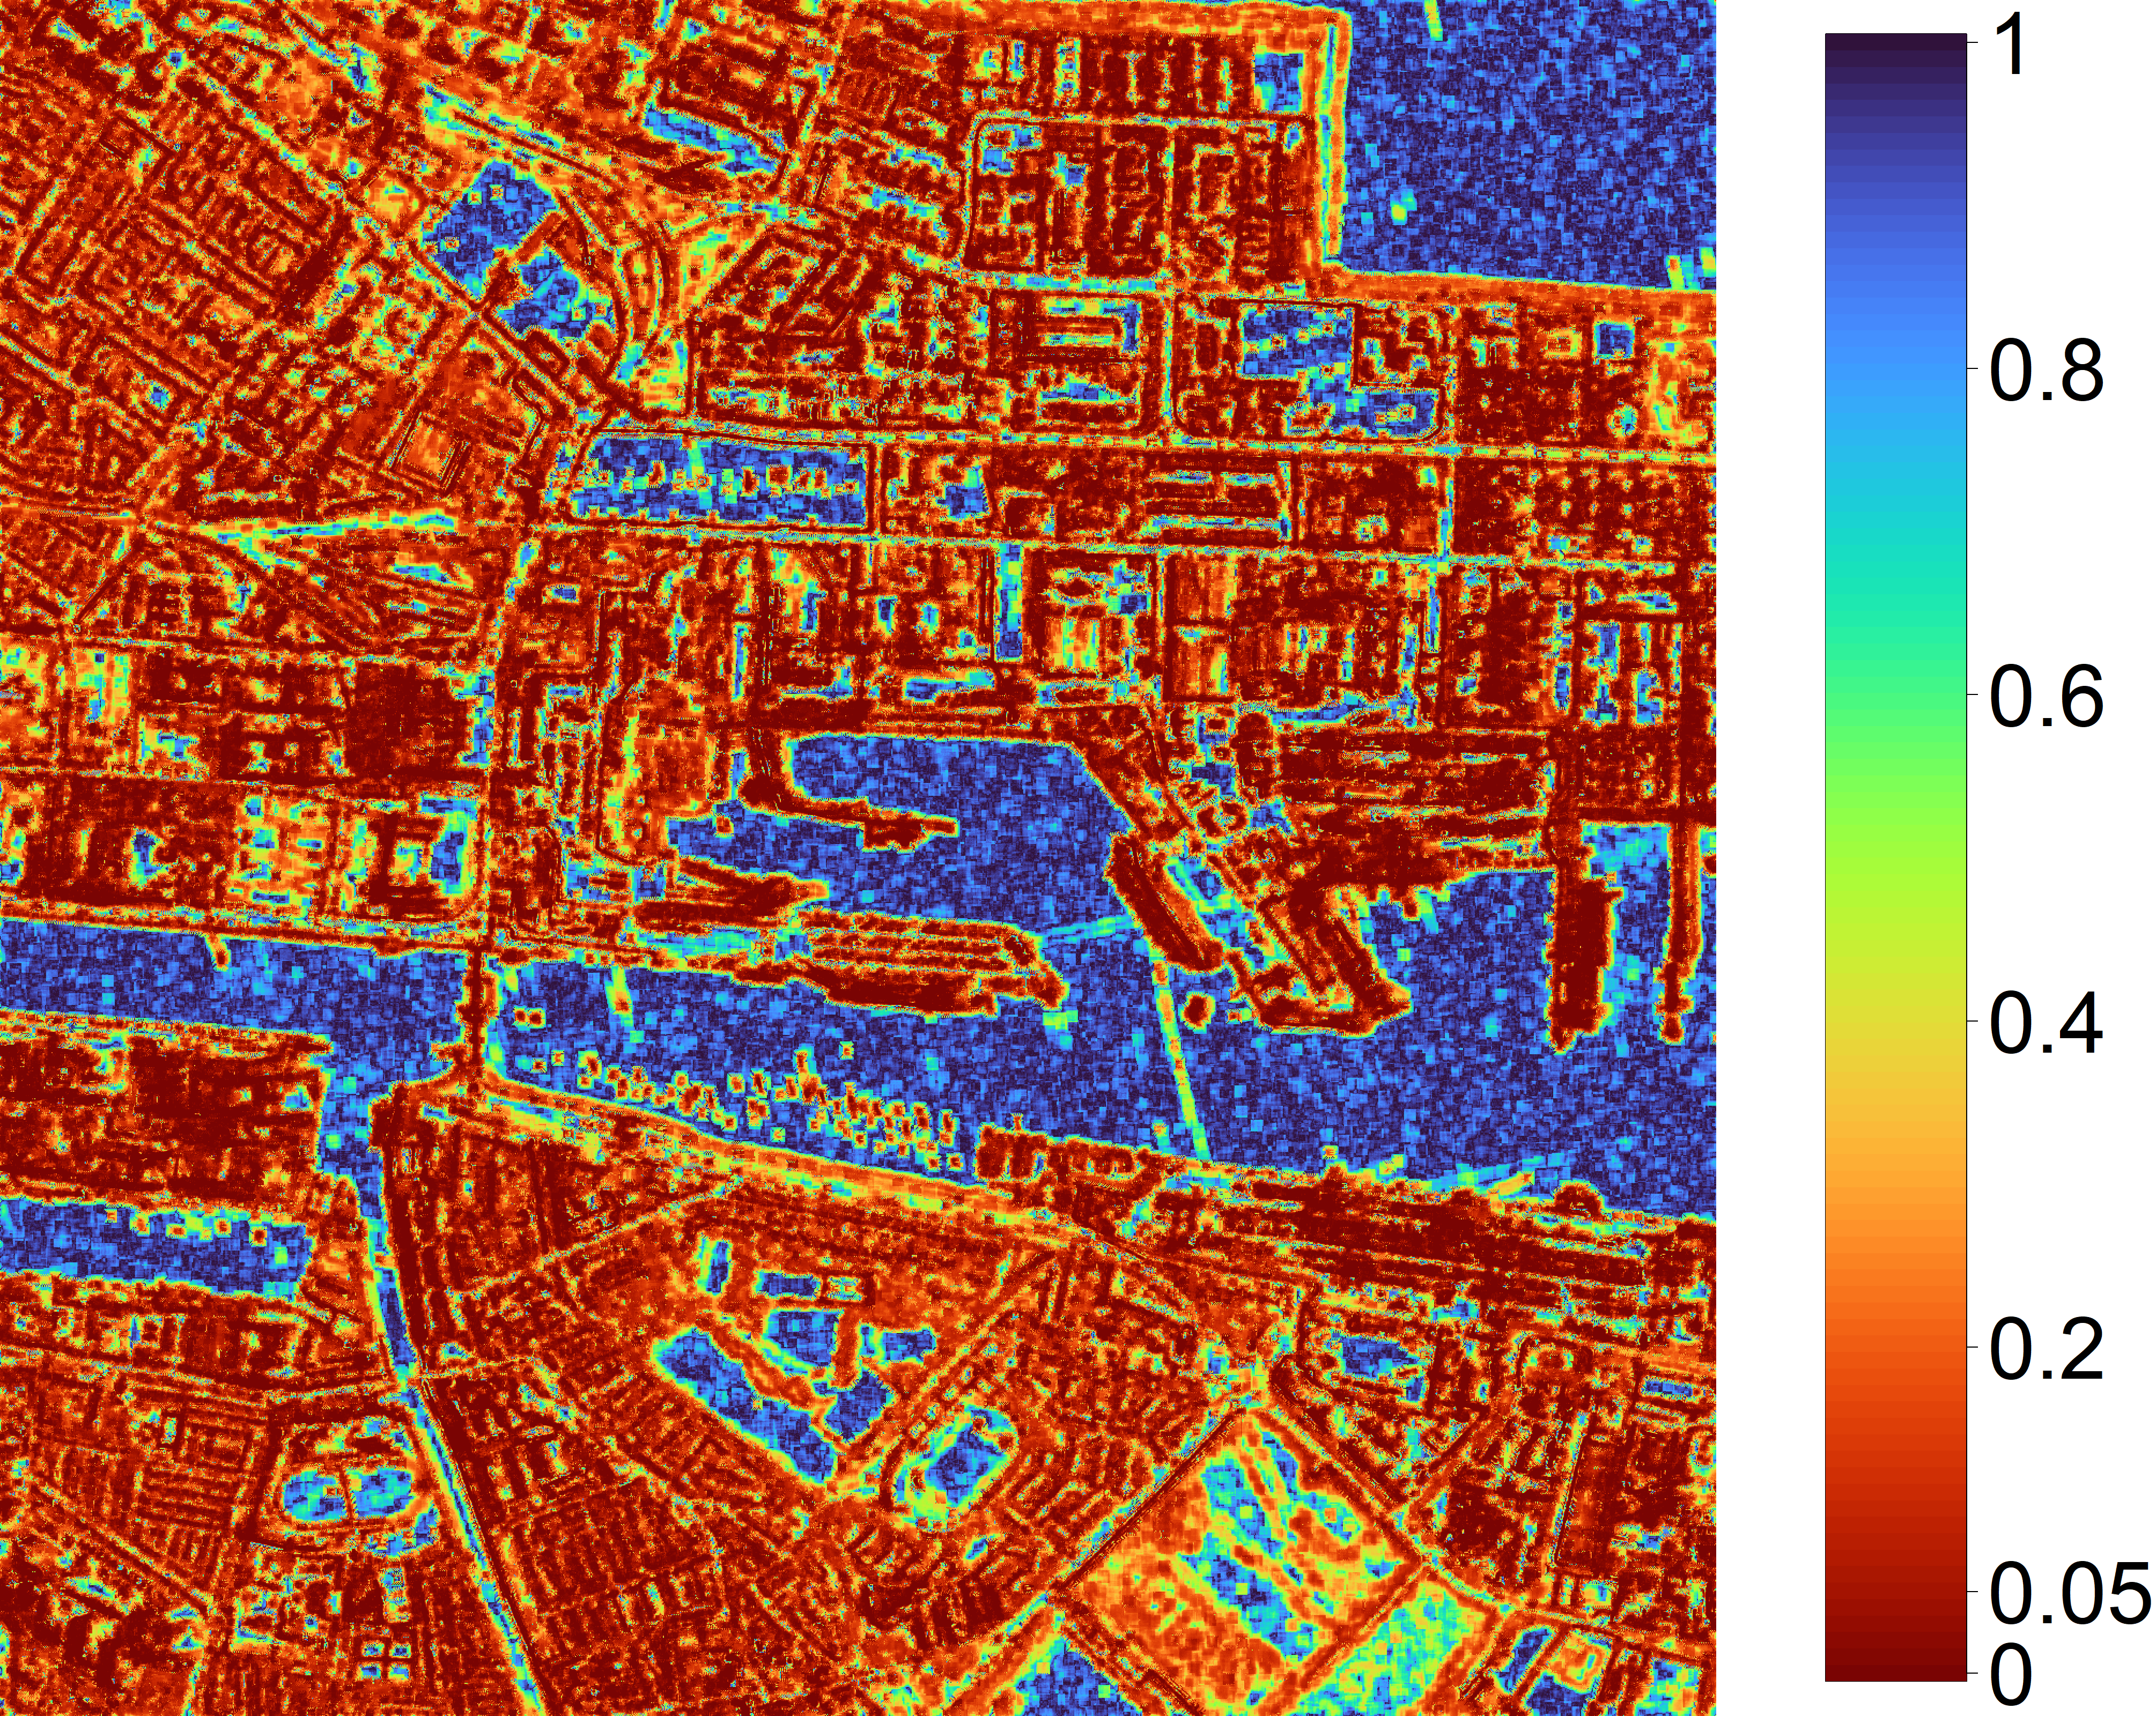
\includegraphics[width=\linewidth]{Figures-R1/dublin_tsallis_adaptive.png}

    \vspace{2pt}
    \textbf{(c)}
\end{minipage}

\caption{(a) Shannon (bootstrap + adaptive), (b) R\'enyi (bootstrap + adaptive), and (c) Tsallis (bootstrap + adaptive) on the Dublin SAR scene.}
\label{fig:dublin_qualitative_comparison}
\end{figure*}

These visual findings are consistent with the quantitative results in
Table~\ref{tbl-dublin-main-benchmark}, where the adaptive bootstrap
Tsallis configuration \DIFdelbegin \DIFdel{attained the best overall performance}\DIFdelend \DIFaddbegin \DIFadd{achieved the highest reported metrics in the
Dublin-scene comparison}\DIFaddend .

\section{Conclusions}\label{sec:conclusion}

This work presented a statistical approach based on the Tsallis entropy
to detect departures from fully-developed speckle in SAR images. The
proposed framework combines a nonparametric entropy-based test,
bootstrap bias correction, and adaptive window selection, yielding
interpretable pixelwise \(p\)-value maps without requiring training data
or explicit estimation of heterogeneous parametric models.

Experiments with simulated and real SAR data showed that the method is
effective in separating homogeneous and heterogeneous regions while
preserving relevant spatial structures. The adaptive strategy improved
the local balance between statistical stability and detail preservation,
and the \DIFdelbegin \DIFdel{null diagnostic }\DIFdelend \DIFaddbegin \DIFadd{analysis under \(\mathcal H_0\) }\DIFaddend confirmed that the adaptive
statistic remains well behaved under homogeneous conditions. The
\DIFdelbegin \DIFdel{refined adaptive
calibration }\DIFdelend \DIFaddbegin \DIFadd{observed-scale standardization }\DIFaddend based on window-dependent centering
\DIFdelbegin \DIFdel{and observed-scale
standardization }\DIFdelend provided a practical and stable formulation for real-scene inference.

The comparative \DIFdelbegin \DIFdel{benchmark on a representative real }\DIFdelend \DIFaddbegin \DIFadd{evaluation on the Dublin }\DIFaddend SAR scene further clarified the
contribution of the proposed method with respect to previous
entropy-based approaches. Under a common evaluation protocol, adaptive
windowing improved all three entropy-based detectors, while the
bootstrap-corrected adaptive Tsallis configuration achieved the \DIFdelbegin \DIFdel{strongest overall performance }\DIFdelend \DIFaddbegin \DIFadd{highest
values for the reported metrics }\DIFaddend among Shannon, Rényi, and Tsallis \DIFaddbegin \DIFadd{in
this benchmark}\DIFaddend .

Although machine learning-based SAR classifiers are widely used, this
framework offers a statistically grounded alternative that provides
interpretable significance measures and requires no labeled data, making
it suitable for rapid detection, screening, and scenarios with limited
data availability.

\appendix[Derivation of the Tsallis Entropy of $\mathcal{G}^0_I$]{}

Starting from the definition of the Tsallis entropy in
\eqref{eq:tsallis} and the pdf that characterizes the
\(\mathcal{G}^0_I(\alpha,\gamma,L)\) model, Eq.~\eqref{E:gi01}, define:
\begin{equation*}
I = \int_0^\infty \left[ f_{\mathcal{G}_I^0}(z) \right]^\lambda \,\mathrm{d}z,
\end{equation*} which, after replacing the density, becomes
\begin{equation*}
I = \left[ \frac{L^L \Gamma(L - \alpha)}{\gamma^\alpha \Gamma(-\alpha) \Gamma(L)} \right]^\lambda 
\int_0^\infty \frac{z^{\lambda(L-1)}}{(\gamma + Lz)^{\lambda(L - \alpha)}}\,\mathrm{d}z.
\DIFdelbegin %DIFDELCMD < \label{eq:J_initial}
%DIFDELCMD < %%%
\DIFdelend \end{equation*} Set \[
C \coloneqq \frac{L^L\,\Gamma(L-\alpha)}{\gamma^\alpha\,\Gamma(-\alpha)\,\Gamma(L)}.
\]

Using \(t = \frac{Lz}{\gamma}\) (so that \(z = \frac{\gamma t}{L}\) and
\(\mathrm{d}z = \frac{\gamma}{L}\,\mathrm{d}t\)), we obtain
\begin{align*}
I &= C^\lambda\,\frac{\gamma}{L}\!
\int_0^\infty \frac{(\gamma t/L)^{\lambda(L-1)}}{[\gamma(1+t)]^{\lambda(L-\alpha)}}\,\mathrm{d}t \notag\\
&= C^\lambda\,\frac{\gamma^{\,1+\lambda(\alpha-1)}}{L^{\,1+\lambda(L-1)}}\!
\int_0^\infty t^{\lambda(L-1)}(1+t)^{-\lambda(L-\alpha)}\,\mathrm{d}t.
\end{align*} By the Beta identity
\(B(a,b)=\int_0^\infty \tfrac{t^{a-1}}{(1+t)^{a+b}}\,\mathrm{d}t=\frac{\Gamma(a)\Gamma(b)}{\Gamma(a+b)}\),
with \[
a=\lambda(L-1)+1,\qquad b=\lambda(1-\alpha)-1,
\] we obtain \begin{equation}
I = \left[ \frac{\Gamma(L - \alpha)}{\Gamma(-\alpha) \Gamma(L)} \right]^\lambda 
\frac{\gamma^{1-\lambda}}{L^{1-\lambda}} 
\frac{\Gamma(a)\Gamma(b)}{\Gamma(a+b)}.
\label{eq:J_beta1}
\end{equation} To express \(I\) in terms of the mean \(\mu\), we use the
relation \(\gamma = -\mu(\alpha + 1)\), valid for \(\alpha < -1\).
Substituting into\DIFdelbegin \DIFdel{\eqref{eq:J_beta1} gives }\begin{displaymath}
\DIFdel{I = }[\DIFdel{-\mu(\alpha + 1)}]\DIFdel{^{1-\lambda} L^{\lambda-1} 
\left[ \frac{\Gamma(L - \alpha)}{\Gamma(-\alpha) \Gamma(L)} \right]^\lambda 
\frac{\Gamma(a)\Gamma(b)}{\Gamma(\lambda(L - \alpha))}.
}\end{displaymath}%DIFAUXCMD
\DIFdelend \DIFaddbegin \DIFadd{~\eqref{eq:J_beta1} gives }\begin{equation}
\DIFadd{I = }[\DIFadd{-\mu(\alpha + 1)}]\DIFadd{^{1-\lambda} L^{\lambda-1} 
\left[ \frac{\Gamma(L - \alpha)}{\Gamma(-\alpha) \Gamma(L)} \right]^\lambda 
\frac{\Gamma(a)\Gamma(b)}{\Gamma(\lambda(L - \alpha))}.
\label{eq:I-GI0-Tsallis}
}\end{equation}\DIFaddend  \DIFdelbegin \DIFdel{Finally, substituting this expression into \eqref{eq:tsallis}, and writing it }\DIFdelend \DIFaddbegin \DIFadd{Substituting~\eqref{eq:I-GI0-Tsallis} into the definition
}\[
\DIFadd{T_\lambda=\frac{1-I}{\lambda-1},
}\] \DIFadd{and writing the result }\DIFaddend in exponential--logarithmic form, we obtain
the \DIFdelbegin \DIFdel{final expression for
\(T_\lambda\bigl(\mathcal{G}^0_I(\alpha, \mu, L)\bigr)\)
in~\eqref{eq:GI0-Tsallis}. }\DIFdelend \DIFaddbegin \DIFadd{direct expression }\begin{multline}
\DIFadd{\label{eq:GI0-Tsallis-direct}
T_\lambda\bigl(\mathcal{G}^0_I(\alpha,\mu,L)\bigr)
=
\frac{1}{\lambda-1}
\Bigl\{1-
\exp\Bigl[
(1-\lambda)\ln\mu
+(\lambda-1)\ln L}\\
\DIFadd{+(1-\lambda)\ln(-\alpha-1)
+\ln\Gamma\bigl(\lambda(L-1)+1\bigr)
-\lambda\ln\Gamma(L)}\\
\DIFadd{+\lambda\ln\Gamma(L-\alpha)
-\lambda\ln\Gamma(-\alpha)
+\ln\Gamma\bigl(\lambda(1-\alpha)-1\bigr)}\\
\DIFadd{-\ln\Gamma\bigl(\lambda(L-\alpha)\bigr)
\Bigr]\Bigr\}.
}\end{multline} \DIFadd{The connection with the homogeneous
\(\Gamma_{\mathrm{SAR}}\) model follows by subtracting the entropy
in~\eqref{eq:gammasar-Tsallis} from the direct expression
in~\eqref{eq:GI0-Tsallis-direct}. This yields the decomposition reported
in~\eqref{eq:GI0-Tsallis}, namely }\begin{equation*}
\DIFadd{T_\lambda\bigl(\mathcal{G}^0_I(\alpha,\mu,L)\bigr)
=
T_\lambda\bigl(\Gamma_{\mathrm{SAR}}(\mu,L)\bigr)
+
\Delta_\lambda(\alpha,\mu,L).
}\end{equation*}
\DIFaddend 

\section*{Computational Information}\label{computational-information}
\addcontentsline{toc}{section}{Computational Information}

This research, including its outputs (e.g., this manuscript), was
executed in \texttt{Quarto} version 1.8.25 and is fully reproducible. We
used \texttt{RStudio} version 2025.09.2+418 and \texttt{R} version
4.5.2. Data and code are available at:
\url{https://github.com/rjaneth/Tsallis_entropy_2025}.

All simulations and SAR image processing were run on a workstation
equipped with an Intel\textsuperscript{\textregistered}
Core\texttrademark{} Ultra 9 285 CPU (\SI{2.5}{\giga\hertz}, 24 cores),
\SI{128}{\giga\byte} RAM, and an NVIDIA\textsuperscript{\textregistered}
GeForce RTX 5090 GPU with \SI{31}{\giga\byte} VRAM, running Windows 11
Pro (24H2).

\section*{References}\label{references}
\addcontentsline{toc}{section}{References}

\phantomsection\label{refs}
\begin{CSLReferences}{0}{0}
\bibitem[\citeproctext]{ref-Mondini2021}
\CSLLeftMargin{{[}1{]} }%
\CSLRightInline{A. C. Mondini, F. Guzzetti, K.-T. Chang, O. Monserrat,
T. R. Martha, and A. Manconi,
{``\href{https://doi.org/10.1016/j.earscirev.2021.103574}{Landslide
failures detection and mapping using synthetic aperture radar: Past,
present and future},''} \emph{Earth-Science Reviews}, vol. 216, p.
103574, 2021. }

\bibitem[\citeproctext]{ref-Amitrano2021}
\CSLLeftMargin{{[}2{]} }%
\CSLRightInline{D. Amitrano \emph{et al.},
{``\href{https://doi.org/10.3390/rs13040604}{Earth environmental
monitoring using multi-temporal synthetic aperture radar: A critical
review of selected applications},''} \emph{Remote Sensing}, vol. 13, no.
4, p. 604, 2021. }

\bibitem[\citeproctext]{ref-Ge2020}
\CSLLeftMargin{{[}3{]} }%
\CSLRightInline{P. Ge, H. Gokon, and K. Meguro,
{``\href{https://doi.org/10.1016/j.rse.2020.111693}{A review on
synthetic aperture radar-based building damage assessment in
disasters},''} \emph{Remote Sensing of Environment}, vol. 240, p.
111693, 2020. }

\bibitem[\citeproctext]{ref-Changan2019}
\CSLLeftMargin{{[}4{]} }%
\CSLRightInline{C. Liu, Z. Chen, Y. Shao, J. Chen, T. Hasi, and H. Pan,
{``\href{https://doi.org/10.1016/s2095-3119(18)62016-7}{Research
advances of SAR remote sensing for agriculture applications: A
review},''} \emph{Journal of Integrative Agriculture}, vol. 18, no. 3,
pp. 506--525, 2019. }

\bibitem[\citeproctext]{ref-Esch2010}
\CSLLeftMargin{{[}5{]} }%
\CSLRightInline{T. Esch, M. Thiel, A. Schenk, A. Roth, A. Muller, and S.
Dech, {``\href{https://doi.org/10.1109/tgrs.2009.2037144}{Delineation of
urban footprints from TerraSAR-{X} data by analyzing speckle
characteristics and intensity information},''} \emph{IEEE Transactions
on Geoscience and Remote Sensing}, vol. 48, no. 2, pp. 905--916, 2010. }

\bibitem[\citeproctext]{ref-NovelTechniquesforBuiltupAreaExtractionfromPolarimetricSARImages2019}
\CSLLeftMargin{{[}6{]} }%
\CSLRightInline{D. Ratha, P. Gamba, A. Bhattacharya, and A. C. Frery,
{``\href{https://doi.org/10.1109/LGRS.2019.2914913}{Novel techniques for
built-up area extraction from polarimetric {SAR} images},''} \emph{IEEE
Geoscience and Remote Sensing Letters}, vol. 17, no. 1, pp. 177--181,
2020. }

\bibitem[\citeproctext]{ref-Cao2024}
\CSLLeftMargin{{[}7{]} }%
\CSLRightInline{S. Cao, C. Zhao, J. Dong, and X. Fu,
{``\href{https://doi.org/10.3390/s24134290}{Ship detection in synthetic
aperture radar images under complex geographical environments, based on
deep learning and morphological networks},''} \emph{Sensors}, vol. 24,
no. 13, p. 4290, 2024. }

\bibitem[\citeproctext]{ref-OntheDetectionandLongTermPathVisualisationofa68Iceberg}
\CSLLeftMargin{{[}8{]} }%
\CSLRightInline{L. Lopez-Lopez, F. Parmiggiani, M. Moctezuma-Flores, and
L. Guerrieri, {``\href{https://doi.org/10.3390/rs13030460}{On the
detection and long-term path visualisation of {A}-68 iceberg},''}
\emph{Remote Sensing}, vol. 13, 2021. }

\bibitem[\citeproctext]{ref-Moreira2013}
\CSLLeftMargin{{[}9{]} }%
\CSLRightInline{A. Moreira, P. Prats-Iraola, M. Younis, G. Krieger, I.
Hajnsek, and K. P. Papathanassiou,
{``\href{https://doi.org/10.1109/mgrs.2013.2248301}{A tutorial on
synthetic aperture radar},''} \emph{IEEE Geoscience and Remote Sensing
Magazine}, vol. 1, no. 1, pp. 6--43, 2013. }

\bibitem[\citeproctext]{ref-Argenti2013}
\CSLLeftMargin{{[}10{]} }%
\CSLRightInline{F. Argenti, A. Lapini, T. Bianchi, and L. Alparone,
{``\href{https://doi.org/10.1109/mgrs.2013.2277512}{A tutorial on
speckle reduction in synthetic aperture radar images},''} \emph{IEEE
Geoscience and Remote Sensing Magazine}, vol. 1, no. 3, pp. 6--35, 2013.
}

\bibitem[\citeproctext]{ref-Baraha2023}
\CSLLeftMargin{{[}11{]} }%
\CSLRightInline{S. Baraha and A. K. Sahoo,
{``\href{https://doi.org/10.1016/j.sigpro.2023.109156}{Synthetic
aperture radar image and its despeckling using variational methods: A
review of recent trends},''} \emph{Signal Processing}, vol. 212, p.
109156, 2023. }

\bibitem[\citeproctext]{ref-ORPSDOuterRectangularProjectionBasedRepresentationforOrientedShipDetectioninSARImages}
\CSLLeftMargin{{[}12{]} }%
\CSLRightInline{M. Zhang, Y. Ouyang, M. Yang, J. Guo, and Y. Li,
{``\href{https://doi.org/10.3390/rs17091511}{{ORPSD}: Outer rectangular
projection-based representation for oriented ship detection in {SAR}
images},''} \emph{Remote Sensing}, vol. 17, no. 9, p. 1511, Apr. 2025. }

\bibitem[\citeproctext]{ref-PDEGuidedDiverseFeatureLearningforSARRotatedShipDetection}
\CSLLeftMargin{{[}13{]} }%
\CSLRightInline{M. Zhang, Z. Yang, J. Guo, and Y. Li,
{``\href{https://doi.org/10.3390/rs17172998}{{PDE}-guided diverse
feature learning for {SAR} rotated ship detection},''} \emph{Remote
Sensing}, vol. 17, no. 17, p. 2998, Aug. 2025. }

\bibitem[\citeproctext]{ref-BurgsVOBurgsAssociatedVertexOffsetEncodingSchemeforDetectingRotatedShipsinSARImages}
\CSLLeftMargin{{[}14{]} }%
\CSLRightInline{M. Zhang, Y. Li, J. Guo, Y. Li, and X. Gao,
{``\href{https://doi.org/10.3390/rs17030388}{{BurgsVO}:
{B}urgs-associated vertex offset encoding scheme for detecting rotated
ships in {SAR} images},''} \emph{Remote Sensing}, vol. 17, no. 3, p.
388, Jan. 2025. }

\bibitem[\citeproctext]{ref-S4DetBreadthandAccurateSineSingleStageShipDetectionforRemoteSenseSARImagery}
\CSLLeftMargin{{[}15{]} }%
\CSLRightInline{M. Zhang, Y. Zhu, L. Li, J. Guo, Z. Liu, and Y. Li,
{``\href{https://doi.org/10.3390/rs17050900}{{S4Det}: Breadth and
accurate sine single-stage ship detection for remote sense {SAR}
imagery},''} \emph{Remote Sensing}, vol. 17, no. 5, p. 900, Mar. 2025. }

\bibitem[\citeproctext]{ref-Frery1997}
\CSLLeftMargin{{[}16{]} }%
\CSLRightInline{A. C. Frery, H.-J. Muller, C. C. F. Yanasse, and S. J.
S. Sant'Anna, {``\href{https://doi.org/10.1109/36.581981}{A model for
extremely heterogeneous clutter},''} \emph{{IEEE} Transactions on
Geoscience and Remote Sensing}, vol. 35, no. 3, pp. 648--659, 1997. }

\bibitem[\citeproctext]{ref-Ferreira2020}
\CSLLeftMargin{{[}17{]} }%
\CSLRightInline{J. De A. Ferreira and A. D. C. Nascimento, {``Shannon
entropy for the {\(\mathcal {G}^0_{I}\)} model: A new segmentation
approach,''} \emph{{IEEE} Journal of Selected Topics in Applied Earth
Observations and Remote Sensing}, vol. 13, pp. 2547--2553, 2020. }

\bibitem[\citeproctext]{ref-Shannon1948}
\CSLLeftMargin{{[}18{]} }%
\CSLRightInline{C. E. Shannon, {``A mathematical theory of
communication,''} \emph{The Bell System Technical Journal}, vol. 27, no.
3, pp. 379--423, 1948. }

\bibitem[\citeproctext]{ref-Nascimento2014}
\CSLLeftMargin{{[}19{]} }%
\CSLRightInline{A. D. C. Nascimento, M. M. Horta, A. C. Frery, and R. J.
Cintra, {``Comparing edge detection methods based on stochastic
entropies and distances for {PolSAR} imagery,''} \emph{{IEEE} Journal of
Selected Topics in Applied Earth Observations and Remote Sensing}, vol.
7, no. 2, pp. 648--663, 2014. }

\bibitem[\citeproctext]{ref-Nobre2016}
\CSLLeftMargin{{[}20{]} }%
\CSLRightInline{R. H. Nobre, F. A. A. Rodrigues, R. C. P. Marques, J. S.
Nobre, J. F. S. R. Neto, and F. N. S. Medeiros,
{``\href{https://doi.org/10.1109/lsp.2016.2606760}{SAR image
segmentation with {R}ényi's entropy},''} \emph{IEEE Signal Processing
Letters}, vol. 23, no. 11, pp. 1551--1555, 2016. }

\bibitem[\citeproctext]{ref-Chan2022}
\CSLLeftMargin{{[}21{]} }%
\CSLRightInline{D. Chan, J. Gambini, and A. C. Frery,
{``\href{https://doi.org/10.3390/rs14030509}{Entropy-based non-local
means filter for single-look SAR speckle reduction},''} \emph{Remote
Sensing}, vol. 14, no. 3, p. 509, 2022. }

\bibitem[\citeproctext]{ref-Frery2024}
\CSLLeftMargin{{[}22{]} }%
\CSLRightInline{A. C. Frery, J. Alpala, and A. D. C. Nascimento,
{``\href{https://doi.org/10.3390/rs16111973}{Identifying heterogeneity
in {SAR} data with new test statistics},''} \emph{Remote Sensing}, vol.
16, no. 11, p. 1973, 2024. }

\bibitem[\citeproctext]{ref-Alpala2025}
\CSLLeftMargin{{[}23{]} }%
\CSLRightInline{J. Alpala, A. D. C. Nascimento, and A. C. Frery,
{``\href{https://doi.org/10.1109/lgrs.2025.3581855}{Quantifying
heterogeneity in SAR imagery with the {R}ényi entropy},''} \emph{IEEE
Geoscience and Remote Sensing Letters}, pp. 1--5, 2025. }

\bibitem[\citeproctext]{ref-Tsallis1988}
\CSLLeftMargin{{[}24{]} }%
\CSLRightInline{C. Tsallis,
{``\href{https://doi.org/10.1007/bf01016429}{Possible generalization of
{B}oltzmann-{G}ibbs statistics},''} \emph{Journal of Statistical
Physics}, vol. 52, no. 1--2, pp. 479--487, 1988. }

\bibitem[\citeproctext]{ref-Park1999}
\CSLLeftMargin{{[}25{]} }%
\CSLRightInline{J.-M. Park, W. J. Song, and W. A. Pearlman,
{``\href{https://doi.org/10.1049/ip-vis:19990550}{Speckle filtering of
SAR images based on adaptive windowing},''} \emph{IEE Proceedings --
Vision, Image, and Signal Processing}, vol. 146, no. 4, p. 191, 1999. }

\bibitem[\citeproctext]{ref-Lampropoulos1999}
\CSLLeftMargin{{[}26{]} }%
\CSLRightInline{G. A. Lampropoulos, A. Drosopoulos, and N. Rey, {``High
resolution radar clutter statistics,''} \emph{IEEE Transactions on
Aerospace and Electronic Systems}, vol. 35, no. 1, pp. 43--60, 1999. }

\bibitem[\citeproctext]{ref-Li2011}
\CSLLeftMargin{{[}27{]} }%
\CSLRightInline{H.-C. Li, W. Hong, Y.-R. Wu, and P.-Z. Fan, {``On the
empirical-statistical modeling of {SAR} images with generalized {G}amma
distribution,''} \emph{IEEE Journal of Selected Topics in Signal
Processing}, vol. 5, no. 3, pp. 386--397, 2011. }

\bibitem[\citeproctext]{ref-Nascimento2024}
\CSLLeftMargin{{[}28{]} }%
\CSLRightInline{A. D. C. Nascimento, J. M. Vasconcelos, R. J. Cintra,
and A. C. Frery,
{``\href{https://doi.org/10.1016/j.isprsjprs.2024.05.009}{Regression
model for speckled data with extreme variability},''} \emph{ISPRS
Journal of Photogrammetry and Remote Sensing}, vol. 213, pp. 1--13,
2024. }

\bibitem[\citeproctext]{ref-Havrda1967}
\CSLLeftMargin{{[}29{]} }%
\CSLRightInline{J. Havrda and F. Charvát, {``Quantification method of
classification processes. Concept of structural \(a\)-entropy,''}
\emph{Kybernetika}, vol. 3, no. 1, pp. 30--35, 1967. }

\bibitem[\citeproctext]{ref-vasicek1976test}
\CSLLeftMargin{{[}30{]} }%
\CSLRightInline{O. Vasicek, {``A test for normality based on sample
entropy,''} \emph{Journal of the Royal Statistical Society Series B:
Statistical Methodology}, vol. 38, no. 1, pp. 54--59, 1976. }

\bibitem[\citeproctext]{ref-Ebrahimi1994}
\CSLLeftMargin{{[}31{]} }%
\CSLRightInline{N. Ebrahimi, K. Pflughoeft, and E. S. Soofi, {``Two
measures of sample entropy,''} \emph{Statistics \& Probability Letters},
vol. 20, no. 3, pp. 225--234, 1994. }

\bibitem[\citeproctext]{ref-AlLabadi2024}
\CSLLeftMargin{{[}32{]} }%
\CSLRightInline{L. Al-Labadi, Z. Chu, and Y. Xu,
{``\href{https://doi.org/10.1007/s00180-024-01507-z}{Advancements in
{R}ényi entropy and divergence estimation for model assessment},''}
\emph{Computational Statistics}, 2024. }

\bibitem[\citeproctext]{ref-Crzcgorzewski1999}
\CSLLeftMargin{{[}33{]} }%
\CSLRightInline{P. Crzcgorzewski and R. Wirczorkowski,
{``\href{https://doi.org/10.1080/03610929908832351}{Entropy-based
goodness-of-fit test for exponentiality},''} \emph{Communications in
Statistics - Theory and Methods}, vol. 28, no. 5, pp. 1183--1202, 1999.
}

\bibitem[\citeproctext]{ref-Alpala2024}
\CSLLeftMargin{{[}34{]} }%
\CSLRightInline{J. Alpala, A. D. C. Nascimento, and A. C. Frery,
{``\href{https://doi.org/10.1109/migars61408.2024.10544448}{Identifying
departures from the fully developed speckle hypothesis in intensity
{SAR} data with non-parametric estimation of the entropy},''} in
\emph{2024 {I}nternational {C}onference on {M}achine {I}ntelligence for
{G}eo{A}nalytics and {R}emote {S}ensing ({MIGARS})}, 2024, pp. 1--4. }

\bibitem[\citeproctext]{ref-VanEs1992}
\CSLLeftMargin{{[}35{]} }%
\CSLRightInline{B. Van Es, {``Estimating functionals related to a
density by a class of statistics based on spacings,''}
\emph{Scandinavian Journal of Statistics}, vol. 19, pp. 61--72, 1992. }

\bibitem[\citeproctext]{ref-MathematicalStatisticsvII2015}
\CSLLeftMargin{{[}36{]} }%
\CSLRightInline{P. J. Bickel and K. A. Doksum, \emph{Mathematical
statistics: Basic ideas and selected topics}, vol. 2. Taylor \& Francis
Inc., 2015. }

\bibitem[\citeproctext]{ref-Gomez2017}
\CSLLeftMargin{{[}37{]} }%
\CSLRightInline{L. Gomez, L. Alvarez, L. Mazorra, and A. C. Frery,
{``\href{https://doi.org/10.1016/j.neucom.2016.08.140}{Fully PolSAR
image classification using machine learning techniques and
reaction-diffusion systems},''} \emph{Neurocomputing}, vol. 255, pp.
52--60, 2017. }

\bibitem[\citeproctext]{ref-Frery2019a}
\CSLLeftMargin{{[}38{]} }%
\CSLRightInline{A. C. Frery and J. Gambini,
{``\href{https://doi.org/10.1007/s11749-019-00658-2}{Comparing samples
from the \({\mathcal {G}}^0\) distribution using a geodesic
distance},''} \emph{TEST}, vol. 29, no. 2, pp. 359--378, 2019. }

\bibitem[\citeproctext]{ref-Neto2023}
\CSLLeftMargin{{[}39{]} }%
\CSLRightInline{J. F. S. R. Neto and F. A. A. Rodrigues,
{``\href{https://doi.org/10.1109/lgrs.2023.3305119}{Improving
log-cumulant-based estimation of heterogeneity information in {SAR}
imagery},''} \emph{{IEEE} Geoscience and Remote Sensing Letters}, vol.
20, pp. 1--5, 2023. }

\end{CSLReferences}

\begin{IEEEbiography}
    [{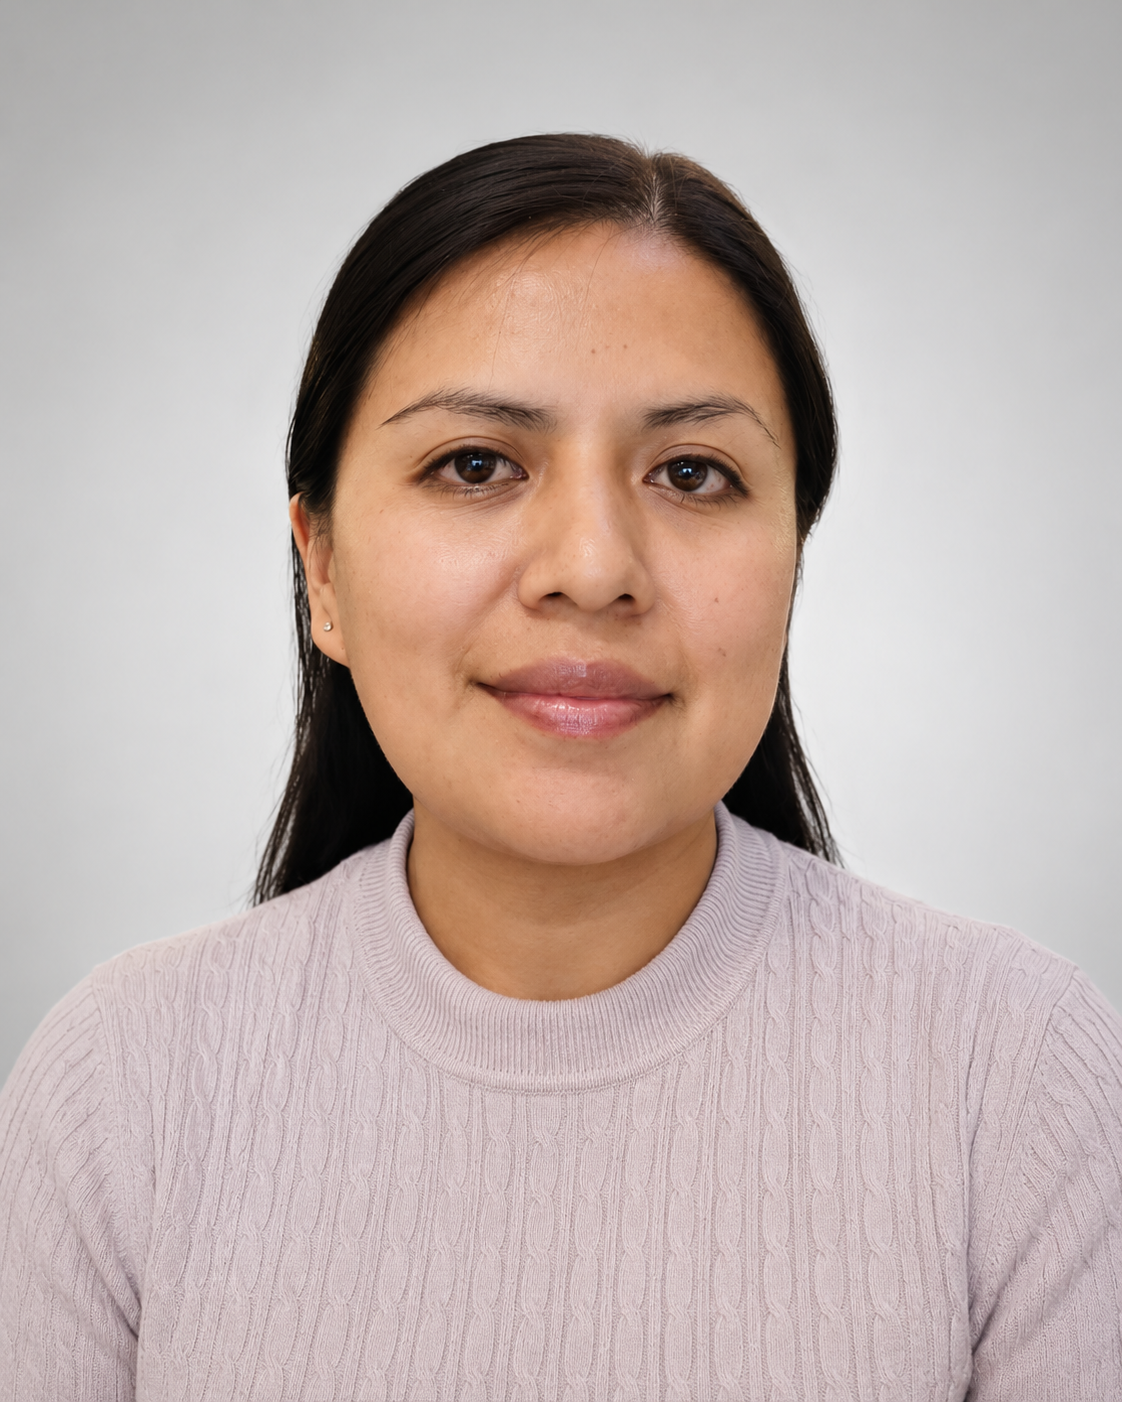
\includegraphics[width=1.05in,clip]{Figures/Janeth.png}}]{Janeth Alpala}
received the B.Sc. degree in Mathematics from the Universidad de Nariño, Colombia, in 2017, the M.Sc. degree in Physics and Mathematics from the Universidad de Granada, Spain, in 2019, and the Ph.D. degree in Statistics from the Universidade Federal de Pernambuco (UFPE), Recife, Brazil, in 2025.
Since August 2025, she has been a Lecturer in Statistics with the Department of Mathematics and Statistics, Universidad de Nariño, Colombia.
Her research interests include statistical computing, statistical information theory, nonparametric entropy estimation, image processing, and synthetic aperture radar data analysis.
\end{IEEEbiography}

\begin{IEEEbiography}
    [{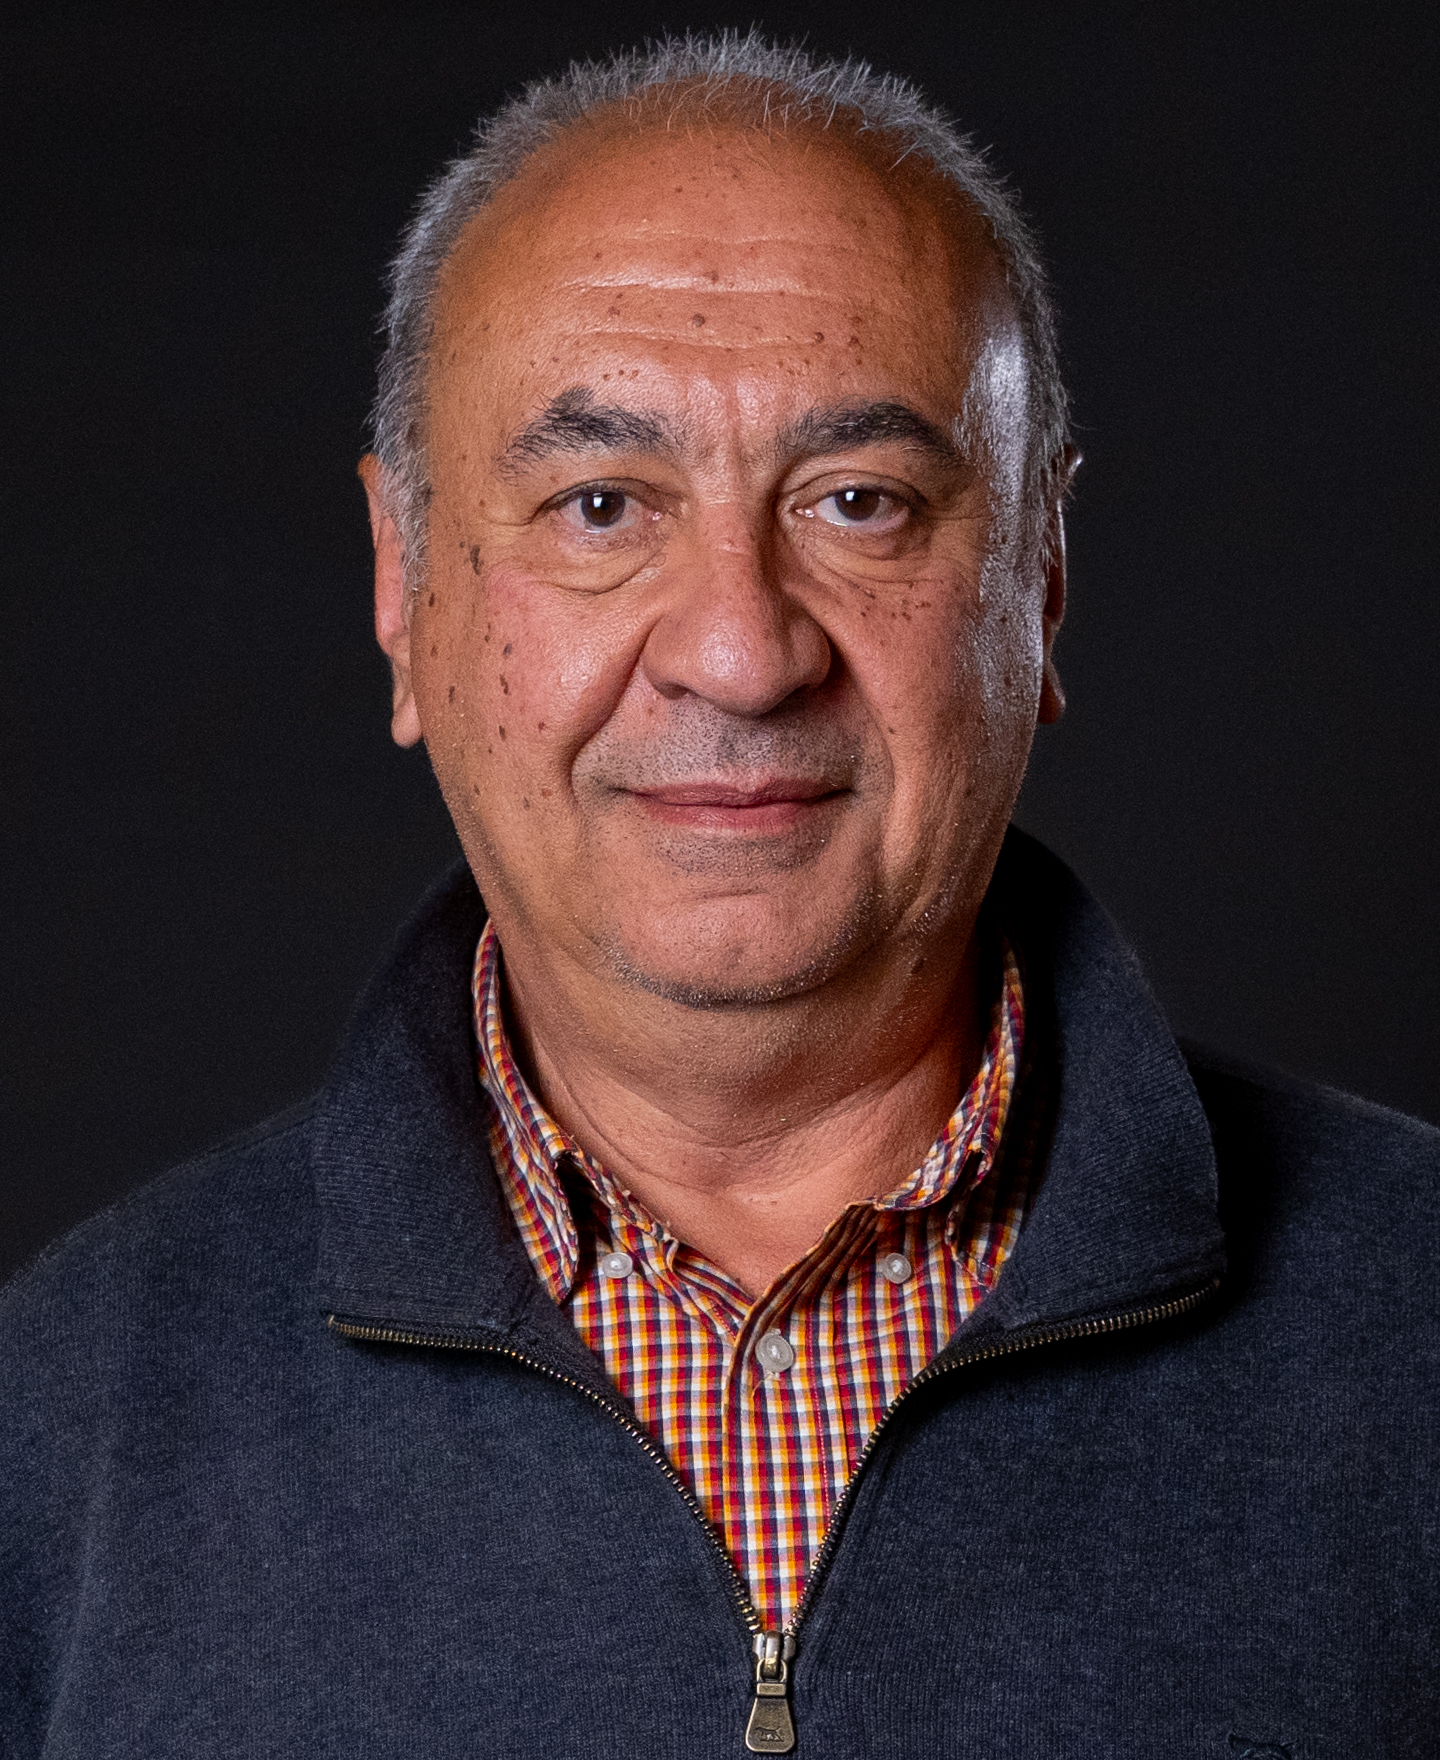
\includegraphics[width=1.05in,clip]{Figures/ACF-IEEE-Face.png}}]{Alejandro C. Frery} 
    (S'91--M'94--SM'14--LF'25) was born in Mendoza, Argentina, in 1960. In 1983, he received a B.Sc. in Electronic and Electrical Engineering from the Universidad de Mendoza. His M.Sc. degree was in Applied Mathematics (Statistics) from the Instituto de Matemática Pura e Aplicada (IMPA, Rio de Janeiro, 1990), and his Ph.D. degree was in Applied Computing from the Instituto Nacional de Pesquisas Espaciais (INPE, São José dos Campos, Brazil, 1993). His research interests are data visualisation, statistical computing, and stochastic modelling, with signal and image processing and networks applications.
    Since May 2020, he has been a Statistics and Data Science Professor at the School of Mathematics and Statistics, Victoria University of Wellington, New Zealand.
    Prof.\ Frery is also a member of the International Society for Photogrammetry and Remote Sensing (ISPRS), the New Zealand Statistical Association, and the Statistical Society of Australia. In 2018, he received the IEEE GRSS Regional Leader Award. After serving as Associate Editor for over five years, Prof. Frery was the Editor-in-Chief of the \textit{IEEE Geoscience and Remote Sensing Letters} from 2014 to 2018. He was an IEEE Geoscience and Remote Sensing Society (GRSS) Distinguished Lecturer from 2015 to 2019. He served as this Society's AdCom (Advisory Committee) member, in charge of Future Publications, Plagiarism and Regional Symposia from 2019 to 2022, and as vice president of Publications from 2023 to 2025.
    Since 2026, he is the vice president for Meetings \& Symposia.
\end{IEEEbiography}

\begin{IEEEbiography}
    [{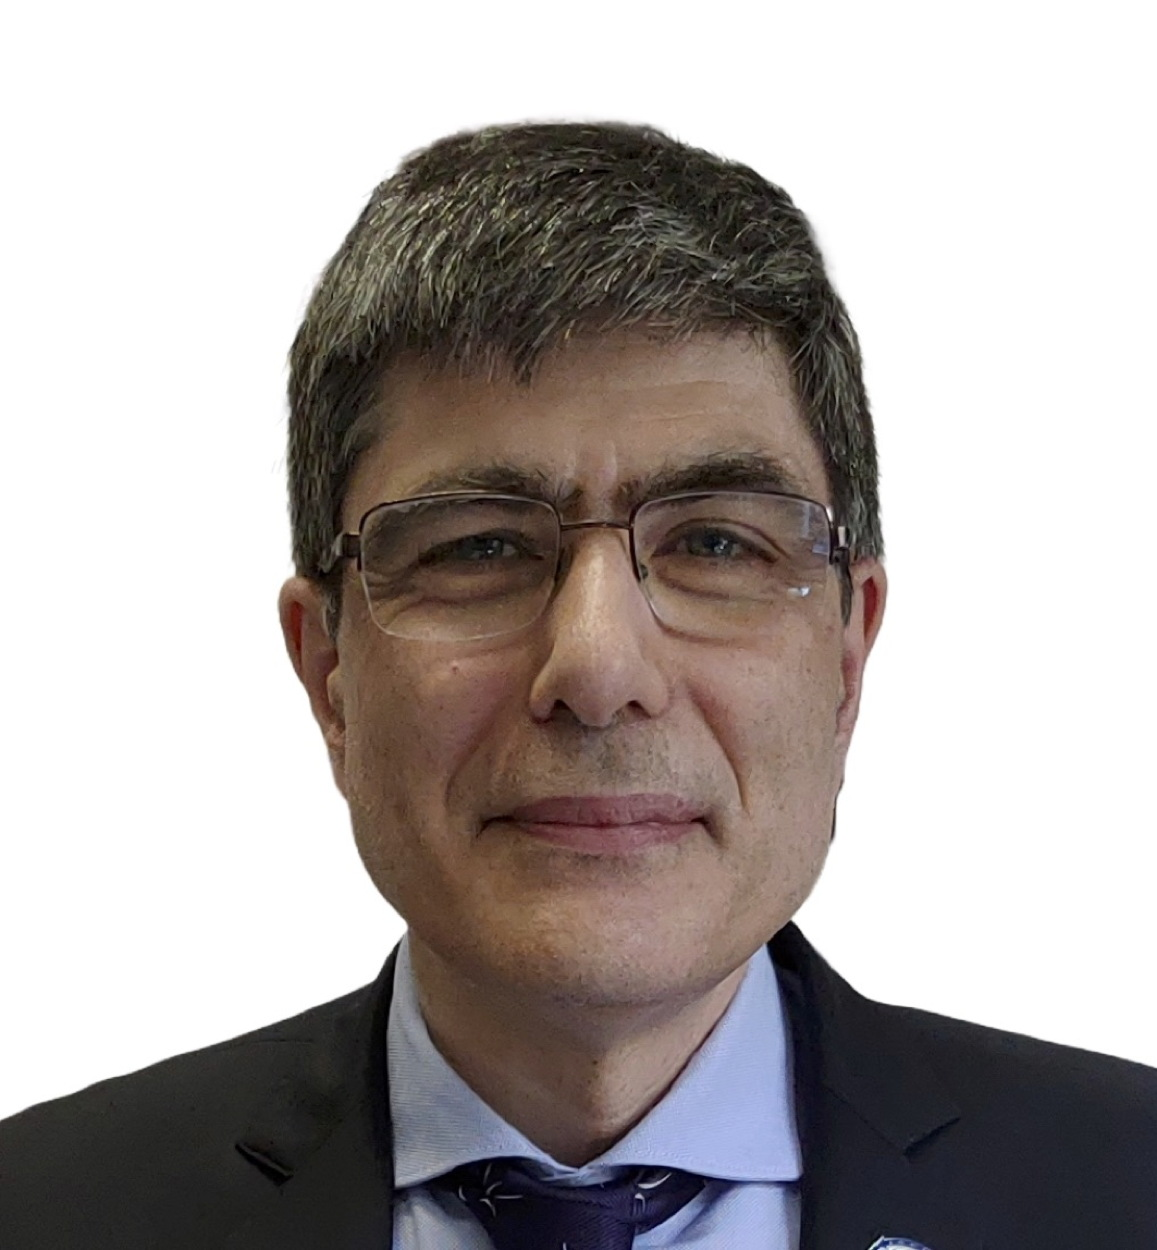
\includegraphics[width=1.05in,clip]{Figures/PG.jpg}}]{Paolo Gamba}
(Fellow, IEEE) is a Professor at the University of Pavia, Italy, in the Telecommunications and Remote Sensing Laboratory. He received the Laurea degree in Electronic Engineering, \textit{cum laude}, from the University of Pavia, Italy, in 1989, and the Ph.D. degree in Electronic Engineering from the same University in 1993.
Prof.\ Gamba served as Editor-in-Chief of the \textit{IEEE Geoscience and Remote Sensing Letters} from 2009 to 2013, as Editor-in-Chief of the \textit{IEEE Geoscience and Remote Sensing Magazine} from 2023 to 2024, and as Chair of the Data Fusion Committee of the IEEE Geoscience and Remote Sensing Society (GRSS) from October 2005 to May 2009. He has been elected in the GRSS AdCom from 2014 to 2022 and served as GRSS President from 2019 to 2020. He also served as Technical Co-Chair of the 2010, 2015, and 2020 IGARSS conferences, in Honolulu, HI, USA, Milan, Italy, and online, respectively.
He is a Fellow of IEEE, IAPR, AAIA, and the Academia Europaea. He has been invited to give keynote lectures and tutorials on several occasions about urban remote sensing, data fusion, EO data for physical exposure, and risk management. He has published more than 240 papers in international peer-reviewed journals.
\end{IEEEbiography}

\begin{IEEEbiography}
    [{
\includegraphics[width=1.05in,clip]{Figures/AbraaoID.jpg}}]{Abraão D. C. Nascimento}
received the B.Sc., M.Sc., and D.Sc. degrees in Statistics from the Universidade Federal de Pernambuco (UFPE), Brazil, in 2005, 2007, and 2012, respectively. Since 2014, he has been an Associate Professor with the Department of Statistics, UFPE. He currently serves as Director of the Graduate Program in Statistics at UFPE and is a researcher in Mathematics, Probability, and Statistics supported by the National Council for Scientific and Technological Development (CNPq), Brazil.
His research interests include statistical information theory, inference for random matrices with emphasis on applications to PolSAR imagery, statistical shape theory, spatio-temporal processes, survival analysis, and asymptotic theory.
\end{IEEEbiography}

\begin{IEEEbiography}
    [{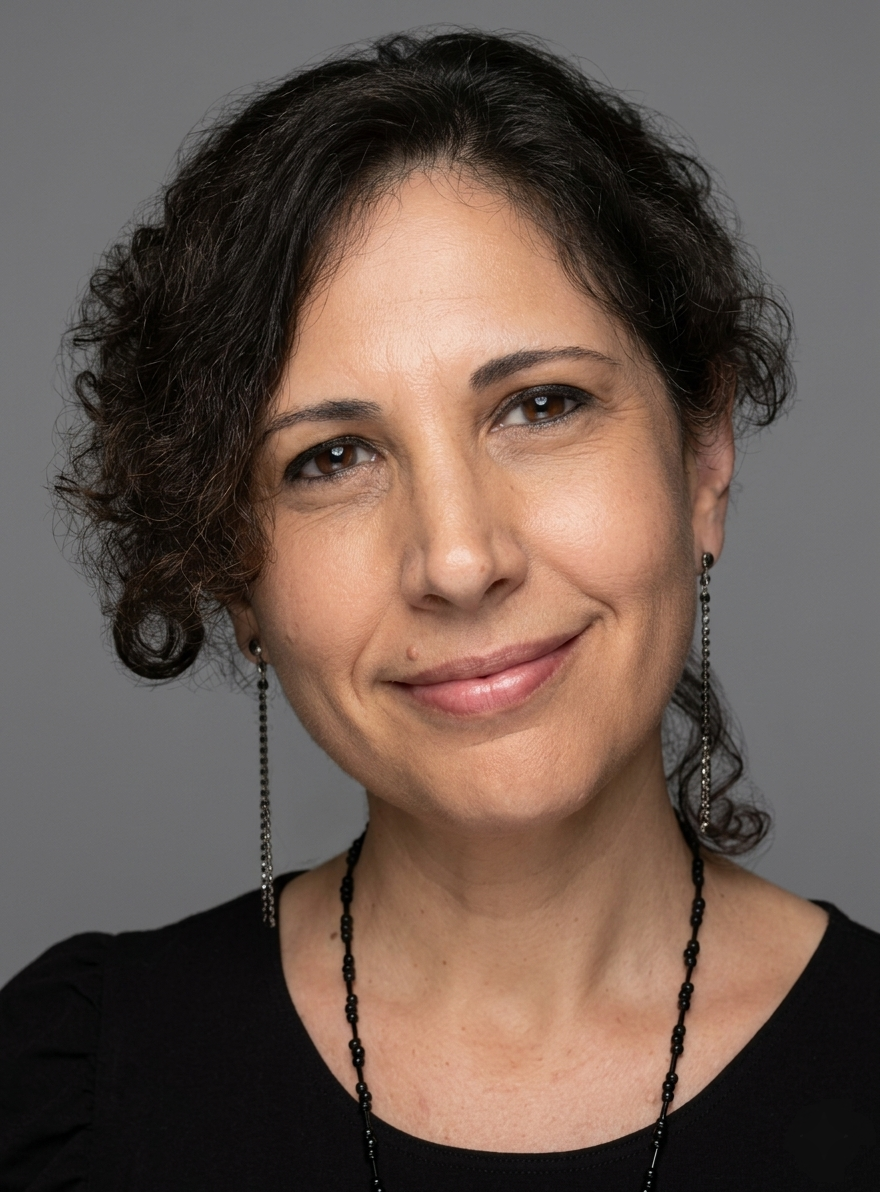
\includegraphics[width=1.05in,clip]{Figures/AARey.png}}]{Andrea A. Rey} 
was born in Mar del Plata, Argentina, in 1978. In 2002, she received a B.Sc. in Mathematics from the Universidad Nacional de Mar del Plata \DIFaddbegin \DIFadd{(UNMDP,  Argentina, 2002)}\DIFaddend . Her Ph.D. degree was in Mathematics from the Universidad de Buenos Aires (UBA,  Argentina, 2009). Her research interests are data science, statistical computing, and machine learning, with signal and image analysis and applications.
Since July 2023, she has been a Full Professor at the Universidad Nacional de Hurlingham (UNAHUR), Argentina.
Prof.\ Rey is also a member of the Laboratorio de Investigación y Desarrollo Experimental en Computación (LIDEC) at the UNAHUR. She has been serving as Associate Editor of the  IEEE Geoscience and Remote Sensing Society (GRSS)  since 2024.
\end{IEEEbiography}


% Can use something like this to put references on a page
% by themselves when using endfloat and the captionsoff option.
\ifCLASSOPTIONcaptionsoff
  \newpage
\fi

% trigger a \newpage just before the given reference
% number - used to balance the columns on the last page
% adjust value as needed - may need to be readjusted if
% the document is modified later
%\IEEEtriggeratref{8}
% The "triggered" command can be changed if desired:
%\IEEEtriggercmd{\enlargethispage{-5in}}

% Uncomment when use biblatex with style=ieee
%\renewcommand{\bibfont}{\footnotesize} % for IEEE bibfont size

\pagebreak[3]
% that's all folks
\end{document}

